\documentclass[twoside,12pt,a4paper,finnish]{book}

%\includeonly{luku13}

\usepackage[finnish,english]{babel}
\usepackage[utf8]{inputenc}
\usepackage{listings}
\usepackage[table]{xcolor}
\usepackage{tikz}
\usepackage{multicol}
\usepackage{hyperref}
\usepackage{array}

\usepackage{fouriernc}
\usepackage[T1]{fontenc}

\usepackage{graphicx}
\usepackage{framed}
\usepackage{amssymb}
\usepackage{amsmath}

\usepackage{pifont}
\usepackage{ifthen}
\usepackage{makeidx}
\usepackage{enumitem}

\usepackage{titlesec}

\usetikzlibrary{patterns,snakes}
\pagestyle{plain}

\lstset{language=C++,frame=single,basicstyle=\ttfamily \small,showstringspaces=false,columns=flexible}
\lstset{
  literate={ö}{{\"o}}1
           {ä}{{\"a}}1
           {ü}{{\"u}}1
}
\lstset{xleftmargin=20pt,xrightmargin=5pt}
\lstset{aboveskip=12pt,belowskip=8pt}


\date{\Large \today}

\usepackage[a4paper,vmargin=30mm,hmargin=33mm,footskip=15mm]{geometry}

\title{\Huge Kisakoodarin käsikirja}
\author{\Large Antti Laaksonen}

\makeindex

\titleformat{\subsubsection}
{\normalfont\large\bfseries\sffamily}{\thesubsection}{1em}{}

\begin{document}

\selectlanguage{finnish}

%\setcounter{page}{1}
%\pagenumbering{roman}

\frontmatter
\maketitle
\setcounter{tocdepth}{1}
\tableofcontents

\chapter*{Alkusanat}
\markboth{\MakeUppercase{Alkusanat}}{}
\addcontentsline{toc}{chapter}{Alkusanat}

Tämän kirjan tarkoituksena on antaa sinulle
perusteellinen johdatus kisakoodauksen maailmaan.
Kirja olettaa, että osaat ennestään
ohjelmoinnin perusasiat, mutta aiempaa kokemusta
kisakoodauksesta ei vaadita.

Kirja on tarkoitettu erityisesti
Datatähti-kilpailun osallistujille,
jotka haluavat oppia algoritmiikkaa
ja mahdollisesti osallistua kansainvälisiin
tietotekniikan olympialaisiin (IOI).
Kirja sopii myös mainiosti 
yliopistojen opiskelijoille ja
kaikille muille kisakoodauksesta kiinnostuneille.

Kirjan lukuihin liittyy kokoelma harjoitustehtäviä,
jotka ovat saatavilla osoitteessa \url{https://cses.fi/dt/list/}.

Hyväksi kisakoodariksi kehittyminen vie aikaa,
mutta se on samalla mahdollisuus oppia paljon.
Voit olla varma, että tulet saamaan hyvän ymmärryksen
algoritmiikan perusteista
kirjaa lukemalla ja tehtäviä ratkomalla.

Kisakoodarin käsikirja on jatkuvan kehityksen alaisena.
Voit lähettää palautetta kirjasta
osoitteeseen
\texttt{ahslaaks@cs.helsinki.fi}.


\mainmatter
\pagenumbering{arabic}
\setcounter{page}{1}

\newcommand{\key}[1] {\textbf{#1}}

\part{Perusasiat}
\chapter{Johdanto}

Kisakoodauksessa yhdistyy kaksi asiaa:
(1) algoritmien suunnittelu ja
(2) algoritmien toteutus.

\key{Algoritmien suunnittelu} on loogista ongelmanratkaisua,
joka on lähellä matematiikkaa.
Se vaatii kykyä analysoida ongelmia ja
ratkaista niitä luovasti.
Tehtävän ratkaisevan algoritmin tulee olla sekä
toimiva että tehokas,
ja usein nimenomaan tehokkaan algoritmin
keksiminen on tehtävän ydin.

Teoreettiset tiedot algoritmiikasta
ovat kisakoodarille kullanarvoisia.
Tyypillisesti tehtävän ratkaisu on yhdistelmä tunnettuja
tekniikoita sekä omia oivalluksia.
Kisakoodauksessa esiintyvät menetelmät ovat myös
algoritmiikan tieteellisen tutkimuksen perusta.

\key{Algoritmien toteutus} edellyttää hyvää ohjelmointitaitoa.
Kisakoodauksessa tehtävän ratkaisun arvostelu tapahtuu
testaamalla toteutettua algoritmia
joukolla testisyötteitä.
Ei siis riitä, että algoritmin idea on oikea,
vaan algoritmi pitää myös onnistua toteuttamaan virheettömästi.

Hyvä kisakoodi on suoraviivaista ja tiivistä.
Ratkaisu täytyy pystyä kirjoittamaan nopeasti,
koska kisoissa on vain vähän aikaa.
Toisin kuin tavallisessa ohjelmistokehityksessä,
ratkaisut ovat lyhyitä
(yleensä enintään joitakin satoja rivejä)
eikä koodia tarvitse ylläpitää kilpailun jälkeen.

\section{Ohjelmointikielet}

\index{ohjelmointikieli@ohjelmointikieli}

Tällä hetkellä yleisimmät koodauskisoissa
käytetyt ohjelmointikielet ovat C++, Python ja Java.
Esimerkiksi vuoden 2016 Google Code Jamissa
3000 parhaan osallistujan joukossa
73 \% käytti C++:aa,
15 \% käytti Pythonia ja
10 \% käytti Javaa\footnote{\url{https://www.go-hero.net/jam/16}}.
Jotkut osallistujat käyttivät myös useita näistä kielistä.

Monen mielestä C++ on paras
valinta kisakoodauksen kieleksi,
ja se on yleensä aina käytettävissä
kisajärjestelmissä.
C++:n etuja ovat, että sillä
toteutettu koodi on hyvin tehokasta
ja kielen standardikirjastoon
kuuluu kattava valikoima valmiita
tietorakenteita ja algoritmeja.

Toisaalta on hyvä hallita useita kieliä
ja tuntea niiden edut.
Esimerkiksi jos tehtävässä esiintyy
suuria kokonaislukuja,
Python voi olla hyvä valinta,
koska kielessä on sisäänrakennettuna
suurten kokonaislukujen käsittely.
Toisaalta tehtävät yritetään yleensä laatia niin,
ettei tietyn kielen ominaisuuksista
ole kohtuutonta etua tehtävän ratkaisussa.

Kaikki tämän kirjan esimerkit on kirjoitettu C++:lla,
ja niissä on käytetty runsaasti C++:n valmiita 
tietorakenteita ja algoritmeja.
Käytössä on C++:n standardi C++11,
jota voi nykyään käyttää useimmissa kisoissa.
Jos et vielä osaa ohjelmoida C++:lla,
nyt on hyvä hetki alkaa opetella.

\subsubsection{C++-koodipohja}

Tyypillinen C++-koodin pohja kisakoodausta varten
näyttää seuraavalta:

\begin{lstlisting}
#include <bits/stdc++.h>

using namespace std;

int main() {
    // koodi tulee tähän
}
\end{lstlisting}

Koodin alussa oleva \texttt{\#include}-rivi
on \texttt{g++}-kääntäjän tarjoama tapa
ottaa mukaan kaikki standardikirjaston sisältö.
Tämän ansiosta koodissa ei tarvitse ottaa
erikseen mukaan kirjastoja \texttt{iostream},
\texttt{vector}, \texttt{algorithm}, jne.,
vaan ne kaikki ovat käytettävissä automaattisesti.

Seuraavana oleva \texttt{using}-rivi määrittää,
että standardikirjaston sisältöä voi käyttää
suoraan koodissa.
Ilman \texttt{using}-riviä koodissa pitäisi
kirjoittaa esimerkiksi \texttt{std::cout},
mutta \texttt{using}-rivin ansiosta riittää
kirjoittaa \texttt{cout}.

Koodin voi kääntää esimerkiksi
seuraavalla komennolla:

\begin{lstlisting}
g++ -std=c++11 -O2 -Wall koodi.cpp -o koodi
\end{lstlisting}

Komento tuottaa kooditiedostosta \texttt{koodi.cpp}
binääritiedoston \texttt{koodi}.
Kääntäjä noudattaa C++11-standardia
(\texttt{-std=c++11}),
optimoi koodia käännöksen aikana (\texttt{-O2})
ja näyttää varoituksia
mahdollisista virheistä (\texttt{-Wall}).

\section{Syöte ja tuloste}

\index{syxte ja tuloste@syöte ja tuloste}

Useimmissa kisoissa käytetään
standardivirtoja syötteen lukemiseen ja tulosteen
kirjoittamiseen.
C++:ssa standardivirrat ovat \texttt{cin}
lukemiseen
ja \texttt{cout} tulostamiseen. Lisäksi voi käyttää
C:n funktioita \texttt{scanf} ja \texttt{printf}.

Ohjelmalle tuleva syöte muodostuu yleensä
luvuista ja merkkijonoista,
joiden välissä on välilyöntejä ja rivinvaihtoja.
Niitä voi lukea \texttt{cin}-virrasta näin:

\begin{lstlisting}
int a, b;
string x;
cin >> a >> b >> x;
\end{lstlisting}

Tällainen koodi toimii aina,
kunhan jokaisen luettavan alkion välissä
on ainakin yksi rivinvaihto tai välilyönti.
Esimerkiksi yllä oleva koodi hyväksyy
molemmat seuraavat syötteet:
\begin{lstlisting}
123 456 apina
\end{lstlisting}
\begin{lstlisting}
123    456
apina
\end{lstlisting}
Tulostaminen tapahtuu puolestaan
\texttt{cout}-virran kautta:
\begin{lstlisting}
int a = 123, b = 456;
string x = "apina";
cout << a << " " << b << " " << x << "\n";
\end{lstlisting}

Syötteen ja tulosteen käsittely on joskus
pullonkaula ohjelmassa.
Seuraavat rivit koodin alussa tehostavat
syötteen ja tulosteen käsittelyä:

\begin{lstlisting}
ios_base::sync_with_stdio(0);
cin.tie(0);
\end{lstlisting}

Huomaa myös, että rivinvaihto \texttt{"\textbackslash n"}
toimii tulostuksessa nopeammin kuin \texttt{endl},
koska \texttt{endl} aiheuttaa
aina flush-operaation.

C:n funktiot \texttt{scanf}
ja \texttt{printf} ovat vaihtoehto
C++:n standardivirroille.
Ne ovat yleensä hieman nopeampia,
mutta toisaalta vaikeakäyttöisempiä.
Seuraava koodi lukee kaksi kokonaislukua syötteestä:
\begin{lstlisting}
int a, b;
scanf("%d %d", &a, &b);
\end{lstlisting}
Seuraava koodi taas tulostaa kaksi kokonaislukua:
\begin{lstlisting}
int a = 123, b = 456;
printf("%d %d\n", a, b);
\end{lstlisting}

Joskus ohjelman täytyy lukea syötteestä
kokonainen rivi tietoa
välittämättä rivin välilyönneistä.
Tämä onnistuu seuraavasti funktiolla
\texttt{getline}:

\begin{lstlisting}
string s;
getline(cin, s);
\end{lstlisting}

Jos syötteessä olevan tiedon määrä ei ole tiedossa
etukäteen, seuraavanlainen silmukka on kätevä:
\begin{lstlisting}
while (cin >> x) {
    // koodia
}
\end{lstlisting}
Tämä silmukka lukee syötettä alkio
kerrallaan, kunnes syöte loppuu.

Joissakin kisajärjestelmissä syötteen ja tulosteen
käsittelyyn käytetään tiedostoja. Helppo ratkaisu tähän
on kirjoittaa koodi tavallisesti
standardivirtoja käyttäen,
mutta kirjoittaa alkuun seuraavat rivit:
\begin{lstlisting}
freopen("input.txt", "r", stdin);
freopen("output.txt", "w", stdout);
\end{lstlisting}
Tämän seurauksena koodi lukee syötteen tiedostosta
''input.txt'' ja kirjoittaa tulosteen
tiedostoon ''output.txt''.

\section{Lukujen käsittely}

\index{kokonaisluku@kokonaisluku}

\subsubsection{Kokonaisluvut}

Tavallisin kokonaislukutyyppi kisakoodauksessa on \texttt{int}.
Tämä on 32-bittinen tyyppi,
jonka sallittu lukuväli on $-2^{31} \ldots 2^{31}-1$
eli noin $-2 \cdot 10^9 \ldots 2 \cdot 10^9$.
Jos tyyppi \texttt{int} ei riitä, sen sijaan voi käyttää
64-bittistä tyyppiä
\texttt{long long}, jonka lukuväli on $-2^{63} \ldots 2^{63}-1$
eli noin $-9 \cdot 10^{18} \ldots 9 \cdot 10^{18}$.

Seuraava koodi määrittelee
\texttt{long long} -muuttujan:
\begin{lstlisting}
long long x = 123456789123456789LL;
\end{lstlisting}
Luvun lopussa oleva \texttt{LL}
ilmaisee, että luku on \texttt{long long} -tyyppinen.

Yleinen virhe \texttt{long long} -tyypin käytössä on,
että jossain kohtaa käytetään kuitenkin \texttt{int}-tyyppiä.
Esimerkiksi tässä koodissa on salakavala virhe:

\begin{lstlisting}
int a = 123456789;
long long b = a*a;
cout << b << "\n"; // -1757895751
\end{lstlisting}

Vaikka muuttuja \texttt{b} on \texttt{long long} -tyyppinen,
laskussa \texttt{a*a} molemmat osat ovat \texttt{int}-tyyppisiä
ja myös laskun tulos on \texttt{int}-tyyppinen.
Tämän vuoksi muuttujaan \texttt{b} ilmestyy väärä luku.
Ongelman voi korjata vaihtamalla muuttujan \texttt{a}
tyypiksi \texttt{long long} tai kirjoittamalla
laskun muodossa \texttt{(long long)a*a}.

Yleensä tehtävät laaditaan niin, että tyypin
\texttt{long long} käyttäminen riittää.
On kuitenkin hyvä tietää, että
\texttt{g++}-kääntäjä tarjoaa myös 128-bittisen
tyypin \texttt{\_\_int128\_t}, jonka lukuväli on
$-2^{127} \ldots 2^{127}-1$ eli noin $-10^{38} \ldots 10^{38}$.
Tämä tyyppi ei kuitenkaan ole käytettävissä kaikissa kisajärjestelmissä.

\subsubsection{Vastaus modulossa}

\index{jakojxxnnos@jakojäännös}
\index{modulolaskenta@modulolaskenta}

Luvun $x$ jakojäännös luvulla $m$
merkitään $x \bmod m$.
Esimerkiksi $17 \bmod 5 = 2$,
koska $17 = 3 \cdot 5 + 2$.

Joskus tehtävän vastaus on hyvin suuri kokonaisluku,
mutta vastaus riittää ilmoittaa ''modulo $m$''
eli vastauksen jakojäännös luvulla $m$
(esimerkiksi ''modulo $10^9+7$'').
Ideana on, että vaikka todellinen vastaus
voi olla hyvin suuri luku,
tehtävässä riittää käyttää tyyppejä \texttt{int} ja \texttt{long long}.

Tärkeä jakojäännöksen ominaisuus on,
että yhteen-, vähennys- ja kertolaskussa
jakojäännöksen voi laskea ennen laskutoimitusta:

\[
\begin{array}{rcr}
(a+b) \bmod m & = & (a \bmod m + b \bmod m) \bmod m \\
(a-b) \bmod m & = & (a \bmod m - b \bmod m) \bmod m \\
(a \cdot b) \bmod m & = & (a \bmod m \cdot b \bmod m) \bmod m
\end{array}
\]

Näiden kaavojen ansiosta
jokaisen laskun vaiheen jälkeen voi laskea jakojäännöksen
eivätkä luvut kasva liian suuriksi.

Esimerkiksi seuraava koodi
laskee luvun $n$ kertoman $n!$ modulo $m$:
\begin{lstlisting}
long long x = 1;
for (int i = 2; i <= n i++) {
    x = (x*i)%m;
}
cout << x << "\n";
\end{lstlisting}

Yleensä vastaus modulossa tulee antaa niin,
että se on välillä $0\ldots m-1$.
Kuitenkin C++:ssa ja
muissa kielissä negatiivisen
luvun jakojäännös voi olla negatiivinen.
Helppo tapa varmistaa, että jakojäännös ei ole negatiivinen,
on laskea ensin jakojäännös tavallisesti ja lisätä sitten $m$,
jos tulos on negatiivinen:
\begin{lstlisting}
x = x%m;
if (x < 0) x += m;
\end{lstlisting}
Tämä on tarpeen kuitenkin vain silloin,
kun jakojäännös voi olla negatiivinen
koodissa olevien vähennyslaskujen vuoksi.

\subsubsection{Liukuluvut}

\index{liukuluku@liukuluku}

Tavalliset liukulukutyypit kisakoodauksessa
ovat 64-bittinen \texttt{double}
sekä \texttt{g++}-kääntäjän
laajennoksena
80-bittinen \texttt{long double}.
Yleensä \texttt{double} riittää,
mutta \texttt{long double} tuo tarvittaessa
lisää tarkkuutta.

Vastauksena oleva liukuluku täytyy yleensä tulostaa
tietyllä tarkkuudella.
Tämä onnistuu helpoiten \texttt{printf}-funktiolla,
jolle voi antaa desimaalien määrän.
Esimerkiksi seuraava koodi tulostaa luvun 9
desimaalin tarkkuudella:

\begin{lstlisting}
printf("%.9f\n", x);
\end{lstlisting}

Liukulukujen käyttämisessä on hankaluutena,
että kaikkia lukuja ei voi esittää tarkasti
liukulukuina vaan tapahtuu pyöristysvirheitä.
Esimerkiksi seuraava koodi tuottaa yllättävän tuloksen:

\begin{lstlisting}
double x = 0.3*3+0.1;
printf("%.20f\n", x); // 0.99999999999999988898
\end{lstlisting}

Pyöristysvirheen vuoksi muuttujan \texttt{x}
sisällöksi tulee hieman alle 1,
vaikka sen arvo tarkasti laskettuna olisi 1.

Liukulukuja on vaarallista vertailla \texttt{==}-merkinnällä,
koska vaikka luvut olisivat todellisuudessa samat,
niissä voi olla pientä eroa pyöristysvirheiden vuoksi.
Parempi tapa vertailla liukulukuja on
tulkita kaksi lukua samoiksi, jos niiden erona on $\varepsilon$,
jossa $\varepsilon$ on sopiva pieni luku.

Käytännössä vertailun voi toteuttaa seuraavasti ($\varepsilon=10^{-9}$):

\begin{lstlisting}
if (abs(a-b) < 1e-9) {
    // a ja b ovat yhtä suuret
}
\end{lstlisting}

Huomaa, että
vaikka liukuluvut ovat epätarkkoja, niillä voi esittää
tarkasti kokonaislukuja tiettyyn rajaan asti.
Esimerkiksi \texttt{double}-tyypillä voi esittää
tarkasti kaikki kokonaisluvut, joiden itseisarvo
on enintään $2^{53}$.

\section{Koodin lyhentäminen}

Kisakoodauksessa ihanteena on lyhyt koodi,
koska algoritmi täytyy pystyä toteuttamaan
mahdollisimman nopeasti.
Monet kisakoodarit käyttävätkin lyhennysmerkintöjä
tietotyypeille ja muille koodin osille.

\subsubsection{Tyyppinimet}
\index{tuppdef@\texttt{typedef}}
Komennolla \texttt{typedef} voi antaa lyhyemmän
nimen tietotyypille.
Esimerkiksi nimi \texttt{long long} on pitkä,
joten tyypille voi antaa lyhyemmän nimen \texttt{ll}:
\begin{lstlisting}
typedef long long ll;
\end{lstlisting}
Tämän jälkeen koodin
\begin{lstlisting}
long long a = 123456789;
long long b = 987654321;
cout << a*b << "\n";
\end{lstlisting}
voi lyhentää seuraavasti:
\begin{lstlisting}
ll a = 123456789;
ll b = 987654321;
cout << a*b << "\n";
\end{lstlisting}

Komentoa \texttt{typedef} voi käyttää myös
monimutkaisempien tyyppien kanssa.
Esimerkiksi seuraava koodi antaa nimen \texttt{vi}
kokonaisluvuista muodostuvalle vektorille
sekä nimen \texttt{pi} kaksi
kokonaislukua sisältävälle parille.
\begin{lstlisting}
typedef vector<int> vi;
typedef pair<int,int> pi;
\end{lstlisting}

\subsubsection{Makrot}
\index{makro}
Toinen tapa lyhentää koodia on määritellä \key{makroja}.
Makro ilmaisee, että tietyt koodissa olevat
merkkijonot korvataan toisilla ennen koodin
kääntämistä.
C++:ssa makro määritellään
esikääntäjän komennolla \texttt{\#define}.

Määritellään esimerkiksi seuraavat makrot:
\begin{lstlisting}
#define F first
#define S second
#define PB push_back
#define MP make_pair
\end{lstlisting}
Tämän jälkeen koodin
\begin{lstlisting}
v.push_back(make_pair(y1,x1));
v.push_back(make_pair(y2,x2));
int d = v[i].first+v[i].second;
\end{lstlisting}
voi kirjoittaa lyhyemmin seuraavasti:
\begin{lstlisting}
v.PB(MP(y1,x1));
v.PB(MP(y2,x2));
int d = v[i].F+v[i].S;
\end{lstlisting}

Makro on mahdollista määritellä myös niin,
että sille voi antaa parametreja.
Tämän ansiosta makrolla voi lyhentää esimerkiksi
komentorakenteita.
Määritellään esimerkiksi seuraava makro:
\begin{lstlisting}
#define REP(i,a,b) for (int i = a; i <= b; i++)
\end{lstlisting}
Tämän jälkeen koodin
\begin{lstlisting}
for (int i = 1; i <= n; i++) {
    haku(i);
}
\end{lstlisting}
voi lyhentää seuraavasti:
\begin{lstlisting}
REP(i,1,n) {
    haku(i);
}
\end{lstlisting}

\section{Matematiikka}

Matematiikka on tärkeässä asemassa kisakoodauksessa,
ja menestyvän kisakoodarin täytyy osata myös
hyvin matematiikkaa.
Käymme seuraavaksi läpi joukon keskeisiä
matematiikan käsitteitä ja kaavoja.
Palaamme moniin aiheisiin myöhemmin tarkemmin kirjan aikana.

\subsubsection{Summakaavat}

Jokaiselle summalle muotoa
\[\sum_{x=1}^n x^k = 1^k+2^k+3^k+\ldots+n^k\]
on olemassa laskukaava,
kun $k$ on jokin positiivinen kokonaisluku.
Tällainen laskukaava on aina astetta $k+1$
oleva polynomi. Esimerkiksi
\[\sum_{x=1}^n x = 1+2+3+\ldots+n = \frac{n(n+1)}{2}\]
ja
\[\sum_{x=1}^n x^2 = 1^2+2^2+3^2+\ldots+n^2 = \frac{n(n+1)(2n+1)}{6}.\]

\key{Aritmeettinen summa} on summa, \index{aritmeettinen summa@aritmeettinen summa}
jossa jokaisen vierekkäisen luvun erotus on vakio.
Esimerkiksi
\[3+7+11+15\]
on aritmeettinen summa,
jossa vakio on 4.
Aritmeettinen summa voidaan laskea kaavalla
\[\frac{n(a+b)}{2},\]
jossa summan ensimmäinen luku on $a$,
viimeinen luku on $b$ ja lukujen määrä on $n$.
Esimerkiksi
\[3+7+11+15=\frac{4 \cdot (3+15)}{2} = 36.\]
Kaava perustuu siihen, että summa muodostuu $n$ luvusta
ja luvun suuruus on keskimäärin $(a+b)/2$.

\index{geometrinen summa@geometrinen summa}
\key{Geometrinen summa} on summa,
jossa jokaisen vierekkäisen luvun suhde on vakio.
Esimerkiksi
\[3+6+12+24\]
on geometrinen summa,
jossa vakio on 2.
Geometrinen summa voidaan laskea kaavalla
\[\frac{bx-a}{x-1},\]
jossa summan ensimmäinen luku on $a$,
viimeinen luku on $b$ ja vierekkäisten lukujen suhde on $x$.
Esimerkiksi
\[3+6+12+24=\frac{24 \cdot 2 - 3}{2-1} = 45.\]

Geometrisen summan kaavan voi johtaa merkitsemällä
\[ S = a + ax + ax^2 + \cdots + b .\] 
Kertomalla molemmat puolet $x$:llä saadaan
\[ xS = ax + ax^2 + ax^3 + \cdots + bx,\]
josta kaava seuraa ratkaisemalla yhtälön
\[ xS-S = bx-a.\]

Geometrisen summan erikoistapaus on usein kätevä kaava
\[1+2+4+8+\ldots+2^{n-1}=2^n-1.\]

% Geometrisen summan sukulainen on
% \[x+2x^2+3x^3+\cdots+k x^k = \frac{kx^{k+2}-(k+1)x^{k+1}+x}{(x-1)^2}. \]

\index{harmoninen summa@harmoninen summa}

\key{Harmoninen summa} on summa muotoa
\[ \sum_{x=1}^n \frac{1}{x} = 1+\frac{1}{2}+\frac{1}{3}+\ldots+\frac{1}{n}.\]

Yläraja harmonisen summan suuruudelle on $\log_2(n)+1$.
Summaa voi näet arvioida ylöspäin
muuttamalla jokaista termiä $1/k$ niin,
että $k$:ksi tulee alempi 2:n potenssi.
Esimerkiksi tapauksessa $n=6$ arvioksi tulee
\[ 1+\frac{1}{2}+\frac{1}{3}+\frac{1}{4}+\frac{1}{5}+\frac{1}{6} \le
1+\frac{1}{2}+\frac{1}{2}+\frac{1}{4}+\frac{1}{4}+\frac{1}{4}.\]
Tämän seurauksena summa jakaantuu $\log_2(n)+1$ osaan
($1$, $2 \cdot 1/2$, $4 \cdot 1/4$, jne.),
joista jokaisen summa on enintään 1.

\subsubsection{Joukko-oppi}

\index{joukko-oppi}
\index{joukko@joukko}
\index{leikkaus@leikkaus}
\index{yhdiste@yhdiste}
\index{erotus@erotus}
\index{osajoukko@osajoukko}
\index{perusjoukko}

\key{Joukko} on kokoelma alkioita.
Esimerkiksi joukko
\[X=\{2,4,7\}\]
sisältää alkiot 2, 4 ja 7.
Merkintä $\emptyset$ tarkoittaa tyhjää joukkoa.
Joukon $S$ koko eli alkoiden määrä on $|S|$.
Esimerkiksi äskeisessä joukossa $|X|=3$.

Merkintä $x \in S$ tarkoittaa,
että alkio $x$ on joukossa $S$,
ja merkintä $x \notin S$ tarkoittaa,
että alkio $x$ ei ole joukossa $S$.
Esimerkiksi äskeisessä joukossa
\[4 \in X \hspace{10px}\textrm{ja}\hspace{10px} 5 \notin X.\]

\begin{samepage}
Uusia joukkoja voidaan muodostaa joukko-operaatioilla
seuraavasti:
\begin{itemize}
\item \key{Leikkaus} $A \cap B$ sisältää alkiot,
jotka ovat molemmissa joukoista $A$ ja $B$.
Esimerkiksi jos $A=\{1,2,5\}$ ja $B=\{2,4\}$,
niin $A \cap B = \{2\}$.
\item \key{Yhdiste} $A \cup B$ sisältää alkiot,
jotka ovat ainakin toisessa joukoista $A$ ja $B$.
Esimerkiksi jos $A=\{3,7\}$ ja $B=\{2,3,8\}$,
niin $A \cup B = \{2,3,7,8\}$.
\item \key{Komplementti} $\bar A$ sisältää alkiot,
jotka eivät ole joukossa $A$.
Komplementin tulkinta riippuu siitä, mikä on
\key{perusjoukko} eli joukko, jossa on kaikki
mahdolliset alkiot. Esimerkiksi jos
$A=\{1,2,5,7\}$ ja perusjoukko on $P=\{1,2,\ldots,10\}$,
niin $\bar A = \{3,4,6,8,9,10\}$.
\item \key{Erotus} $A \setminus B = A \cap \bar B$ sisältää alkiot,
jotka ovat joukossa $A$ mutta eivät joukossa $B$.
Huomaa, että $B$:ssä voi olla alkioita,
joita ei ole $A$:ssa.
Esimerkiksi jos $A=\{2,3,7,8\}$ ja $B=\{3,5,8\}$,
niin $A \setminus B = \{2,7\}$.
\end{itemize}
\end{samepage}


Merkintä $A \subset S$ tarkoittaa,
että $A$ on $S$:n \key{osajoukko}
eli jokainen $A$:n alkio esiintyy $S$:ssä.
Joukon $S$ osajoukkojen yhteismäärä on $2^{|S|}$.
Esimerkiksi joukon $\{2,4,7\}$
osajoukot ovat
\begin{center}
$\emptyset$,
$\{2\}$, $\{4\}$, $\{7\}$, $\{2,4\}$, $\{2,7\}$, $\{4,7\}$ ja $\{2,4,7\}$.
\end{center}

Usein esiintyviä joukkoja ovat

\begin{itemize}[noitemsep]
\item $\mathbb{N}$ (luonnolliset luvut),
\item $\mathbb{Z}$ (kokonaisluvut),
\item $\mathbb{Q}$ (rationaaliluvut) ja
\item $\mathbb{R}$ (reaaliluvut).
\end{itemize}

Luonnollisten lukujen joukko $\mathbb{N}$ voidaan määritellä
tilanteesta riippuen kahdella tavalla:
joko $\mathbb{N}=\{0,1,2,\ldots\}$
tai $\mathbb{N}=\{1,2,3,...\}$.

Joukon voi muodostaa myös säännöllä muotoa
\[\{f(n) : n \in S\},\]
missä $f(n)$ on jokin funktio.
Tällainen joukko sisältää kaikki alkiot
$f(n)$, jossa $n$ on valittu joukosta $S$.
Esimerkiksi joukko
\[X=\{2n : n \in \mathbb{Z}\}\]
sisältää kaikki parilliset kokonaisluvut.

\subsubsection{Logiikka}

\index{logiikka@logiikka}
\index{negaatio@negaatio}
\index{konjunktio@konjunktio}
\index{disjunktio@disjunktio}
\index{implikaatio@implikaatio}
\index{ekvivalenssi@ekvivalenssi}

Loogisen lausekkeen arvo on joko \key{tosi} (1) tai
\key{epätosi} (0).
Tärkeimmät loogiset operaatiot ovat
$\lnot$ (\key{negaatio}),
$\land$ (\key{konjunktio}),
$\lor$ (\key{disjunktio}),
$\Rightarrow$ (\key{implikaatio}) sekä
$\Leftrightarrow$ (\key{ekvivalenssi}).
Seuraava taulukko näyttää operaatioiden merkityksen:

\begin{center}
\begin{tabular}{rr|rrrrrrr}
$A$ & $B$ & $\lnot A$ & $\lnot B$ & $A \land B$ & $A \lor B$ & $A \Rightarrow B$ & $A \Leftrightarrow B$ \\
\hline
0 & 0 & 1 & 1 & 0 & 0 & 1 & 1 \\
0 & 1 & 1 & 0 & 0 & 1 & 1 & 0 \\
1 & 0 & 0 & 1 & 0 & 1 & 0 & 0 \\
1 & 1 & 0 & 0 & 1 & 1 & 1 & 1 \\
\end{tabular}
\end{center}

Negaatio $\lnot A$ muuttaa lausekkeen käänteiseksi.
Lauseke $A \land B$ on tosi, jos molemmat $A$ ja $B$ ovat tosia,
ja lauseke $A \lor B$ on tosi, jos $A$ tai $B$ on tosi.
Lauseke $A \Rightarrow B$ on tosi,
jos $A$:n ollessa tosi myös $B$:n on aina tosi.
Lauseke $A \Leftrightarrow B$ on tosi,
jos $A$:n ja $B$:n totuusarvo on sama.

\index{predikaatti@predikaatti}

\key{Predikaatti} on lauseke, jonka arvo on tosi tai epätosi
riippuen sen parametreista.
Yleensä predikaattia merkitään suurella kirjaimella.
Esimerkiksi voimme määritellä predikaatin $P(x)$,
joka on tosi tarkalleen silloin, kun $x$ on alkuluku.
Tällöin esimerkiksi $P(7)$ on tosi, kun taas $P(8)$ on epätosi.

\index{kvanttori@kvanttori}

\key{Kvanttori} ilmaisee, että looginen
lauseke liittyy jollakin tavalla joukon alkioihin.
Tavalliset kvanttorit
ovat $\forall$ (\key{kaikille}) ja $\exists$ (\key{on olemassa}).
Esimerkiksi
\[\forall x (\exists y (y < x))\]
tarkoittaa, että jokaiselle joukon
alkiolle $x$ on olemassa
jokin joukon alkio $y$ niin, että $y$ on $x$:ää pienempi.
Tämä lauseke on tosi kokonaislukujen joukossa,
mutta epätosi luonnollisten lukujen joukossa.

Yllä esitettyjen merkintöjä avulla on mahdollista esittää
monenlaisia loogisia väitteitä.
Esimerkiksi
\[\forall x (\lnot P(x) \Rightarrow (\exists a (\exists b (x = ab \land a > 1 \land b > 1))))\]
tarkoittaa kokonaislukujen joukossa, että jos luku $x$ ei ole alkuluku,
niin on olemassa luvut $a$ ja $b$,
joiden tulo on $x$ ja jotka molemmat ovat suurempia kuin 1.
Tämän lausekkeen arvo on tosi.

\subsubsection{Funktioita}

Funktio $\lfloor x \rfloor$ pyöristää luvun $x$
alaspäin kokonaisluvuksi ja
funktio $\lceil x \rceil$ pyöristää luvun $x$
ylöspäin kokonaisluvuksi. Esimerkiksi
\[ \lfloor 3/2 \rfloor = 1 \hspace{10px} \textrm{ja} \hspace{10px} \lceil 3/2 \rceil = 2.\]

Funktiot $\min(x_1,x_2,\ldots,x_n)$
ja $\max(x_1,x_2,\ldots,x_n)$
palauttavat pienimmän ja suurimman
arvoista $x_1,x_2,\ldots,x_n$.
Esimerkiksi
\[ \min(1,2,3)=1 \hspace{10px} \textrm{ja} \hspace{10px} \max(1,2,3)=3.\]

\index{kertoma@kertoma}

\key{Kertoma} $n!$ määritellään
\[\prod_{x=1}^n x = 1 \cdot 2 \cdot 3 \cdot \ldots \cdot n\]
eli toisin sanoen rekursiivisesti
\[
\begin{array}{lcl}
0! & = & 1 \\
n! & = & n \cdot (n-1)! \\
\end{array}
\]

\index{Fibonaccin luku@Fibonaccin luku}

\key{Fibonaccin luvut} esiintyvät monissa erilaisissa yhteyksissä.
Ne määritellään seuraavasti rekursiivisesti:
\[
\begin{array}{lcl}
f(0) & = & 0 \\
f(1) & = & 1 \\
f(n) & = & f(n-1)+f(n-2) \\
\end{array}
\]
Ensimmäiset Fibonaccin luvut ovat
\[0, 1, 1, 2, 3, 5, 8, 13, 21, 34, 55, \ldots\]
Fibonaccin lukujen laskemiseen on olemassa myös
suljetun muodon kaava
\[f(n)=\frac{(1 + \sqrt{5})^n - (1-\sqrt{5})^n}{2^n \sqrt{5}}.\]

\subsubsection{Logaritmi}

\index{logaritmi@logaritmi}

Luvun $x$
\key{logaritmi} merkitään $\log_k(x)$, missä $k$ on logaritmin kantaluku.
Logaritmin määritelmän mukaan
$\log_k(x)=a$ tarkalleen silloin, kun $k^a=x$.

Algoritmiikassa hyödyllinen tulkinta on,
että logaritmi $\log_k(x)$ ilmaisee, montako kertaa lukua $x$
täytyy jakaa $k$:lla, ennen kuin tulos on 1.
Esimerkiksi $\log_2(32)=5$,
koska lukua 32 täytyy jakaa 2:lla 5 kertaa:

\[32 \rightarrow 16 \rightarrow 8 \rightarrow 4 \rightarrow 2 \rightarrow 1 \]

Logaritmi tulee usein vastaan algoritmien analyysissa,
koska monessa tehokkaassa algoritmissa jokin asia puolittuu
joka askeleella.
Niinpä logaritmin avulla voi arvioida algoritmin tehokkuutta.

Logaritmille pätee kaava
\[\log_k(ab) = \log_k(a)+\log_k(b),\]
josta seuraa edelleen
\[\log_k(x^n) = n \cdot \log_k(x).\]
Samoin logaritmille pätee
\[\log_k\Big(\frac{a}{b}\Big) = \log_k(a)-\log_k(b).\]
Lisäksi on voimassa kaava
\[\log_u(x) = \frac{\log_k(x)}{\log_k(u)},\]
minkä ansiosta logaritmeja voi laskea mille tahansa kantaluvulle,
jos on keino laskea logaritmeja jollekin kantaluvulle.

\index{luonnollinen logaritmi@luonnollinen logaritmi}
\index{Neperin luku@Neperin luku}

Luvun $x$ \key{luonnollinen logaritmi} $\ln(x)$ on logaritmi, jonka kantaluku on
\key{Neperin luku} $e \approx 2{,}71828$.

Vielä yksi logaritmin ominaisuus on, että
luvun $x$ numeroiden määrä $b$-kantaisessa
lukujärjestelmässä
on $\lfloor \log_b(x)+1 \rfloor$.
Esimerkiksi luvun $123$ esitys
2-järjestelmässä on 1111011 ja
$\lfloor \log_2(123)+1 \rfloor = 7$.


\chapter{Aikavaativuus}

\index{aikavaativuus}

Kisakoodauksessa oleellinen asia on algoritmien tehokkuus.
Yleensä on helppoa suunnitella algoritmi,
joka ratkaisee tehtävän hitaasti,
mutta todellinen vaikeus piilee siinä,
kuinka keksiä nopeasti toimiva algoritmi.
Jos algoritmi on liian hidas, se tuottaa vain
osan pisteistä tai ei pisteitä lainkaan.

Aikavaativuus (\textit{time complexity}) on kätevä tapa arvioida,
kuinka nopeasti algoritmi toimii.
Se arvioi algoritmin tehokkuutta funktiona,
jonka parametrina on syötteen koko.
Aikavaativuuden avulla algoritmista voi päätellä ennen koodaamista,
onko se riittävän tehokas tehtävän ratkaisuun.

\section{Laskusäännöt}

Algoritmin aikavaativuus merkitään $O(\cdots)$,
jossa kolmen pisteen tilalla
on kaava, joka kuvaa algoritmin ajankäyttöä.
Yleensä muuttuja $n$ esittää syötteen kokoa.
Esimerkiksi jos algoritmin syötteenä on taulukko lukuja,
$n$ on lukujen määrä,
ja jos syötteenä on merkkijono,
$n$ on merkkijonon pituus.

\subsubsection*{Silmukat}

Algoritmin ajankäyttö johtuu usein
pohjimmiltaan silmukoista,
jotka käyvät syötettä läpi.
Mitä enemmän sisäkkäisiä silmukoita
algoritmissa on, sitä hitaampi se on.
Jos sisäkkäisiä silmukoita on $k$,
aikavaativuus on $O(n^k)$.

Esimerkiksi seuraavan koodin aikavaativuus on $O(n)$:
\begin{lstlisting}
for (int i = 1; i <= n; i++) {
    // koodia
}
\end{lstlisting}

Vastaavasti seuraavan koodin aikavaativuus on $O(n^2)$:
\begin{lstlisting}
for (int i = 1; i <= n; i++) {
    for (int j = 1; j <= n; j++) {
        // koodia
    }
}
\end{lstlisting}

\subsubsection*{Suuruusluokka}

Aikavaativuus ei kerro tarkasti,
montako kertaa silmukan sisällä oleva koodi suoritetaan,
vaan se kertoo vain suuruusluokan.
Esimerkiksi seuraavissa esimerkeissä silmukat
suoritetaan $3n$, $n+5$ ja $\lfloor n/2 \rfloor$ kertaa,
mutta kunkin koodin aikavaativuus on sama $O(n)$.

\begin{lstlisting}
for (int i = 1; i <= 3*n; i++) {
    // koodia
}
\end{lstlisting}

\begin{lstlisting}
for (int i = 1; i <= n+5; i++) {
    // koodia
}
\end{lstlisting}

\begin{lstlisting}
for (int i = 1; i <= n; i += 2) {
    // koodia
}
\end{lstlisting}

Seuraavan koodin aikavaativuus on $O(n^2)$,
koska silmukoiden sisällä oleva
koodi suoritetaan $1+2+\cdots+n = \frac{n(n+1)}{2}$ kertaa.

\begin{lstlisting}
for (int i = 1; i <= n; i++) {
    for (int j = 1; j <= i; j++) {
        // koodia
    }
}
\end{lstlisting}

\subsubsection*{Peräkkäisyys}

Jos koodissa on peräkkäisiä osia,
kokonaisaikavaativuus on suurin yksittäisen
osan aikavaativuus.
Tämä johtuu siitä, että koodin hitain
vaihe on yleensä koodin pullonkaula
ja muiden vaiheiden merkitys on pieni.

Esimerkiksi seuraava koodi muodostuu
kolmesta osasta,
joiden aikavaativuudet ovat $O(n)$, $O(n^2)$ ja $O(n)$.
Niinpä koodin aikavaativuus on $O(n^2)$.

\begin{lstlisting}
for (int i = 1; i <= n; i++) {
    // koodia
}
for (int i = 1; i <= n; i++) {
    for (int j = 1; j <= n; j++) {
        // koodia
    }
}
for (int i = 1; i <= n; i++) {
    // koodia
}
\end{lstlisting}

\subsubsection*{Monta muuttujaa}

Joskus syötteessä on monta muuttujaa,
jotka vaikuttavat aikavaativuuteen.
Tällöin myös aikavaativuuden kaavassa esiintyy
monta muuttujaa.

Esimerkiksi seuraavan koodin
aikavaativuus on $O(nm)$:

\begin{lstlisting}
for (int i = 1; i <= n; i++) {
    for (int j = 1; j <= m; j++) {
        // koodia
    }
}
\end{lstlisting}

\subsubsection*{Rekursio}

Rekursiivisen funktion aikavaativuuden
määrittää, montako kertaa funktiota kutsutaan yhteensä
ja mikä on yksittäisen kutsun aikavaativuus.
Kokonais\-aikavaativuus saadaan kertomalla
nämä arvot toisillaan.

Tarkastellaan esimerkiksi seuraavaa funktiota:

\begin{lstlisting}
void f(int n) {
    if (n == 1) return;
    f(n-1);
}
\end{lstlisting}
Kutsu $\texttt{f}(n)$ aiheuttaa yhteensä $n$ funktiokutsua,
ja jokainen funktiokutsu vie vakioajan,
joten aikavaativuus on $O(n)$.

Tarkastellaan sitten seuraavaa funktiota:

\begin{lstlisting}
void g(int n) {
    if (n == 1) return;
    g(n-1);
    g(n-1);
}
\end{lstlisting}

Tässä tapauksessa funktio haarautuu kahteen osaan,
joten kutsu $\texttt{g}(n)$ aiheuttaa kaikkiaan seuraavat kutsut:

\begin{center}
\begin{tabular}{rr}
kutsu & kerrat \\
\hline
$\texttt{g}(n)$ & 1 \\
$\texttt{g}(n-1)$ & 2 \\
$\texttt{g}(n-2)$ & 4 \\
$\cdots$ & $\cdots$ \\
$\texttt{g}(1)$ & $2^{n-1}$ \\

\end{tabular}
\end{center}

Tämän perusteella kutsun $\texttt{g}(n)$ aikavaativuus on

\[1+2+4+\cdots+2^{n-1} = 2^n-1 = O(2^n).\]

\section{Vaativuusluokkia}

\index{vaativuusluokka}

\subsubsection*{$O(1)$ (vakioaikainen)}

Aikavaativuus $O(1)$ tarkoittaa,
että algoritmi on vakioaikainen
eli algoritmin nopeus ei riipu syötteen koosta.
Tyypillinen $O(1)$-algoritmi on suora kaava
vastauksen laskemiseen.

\subsubsection*{$O(\log n)$ (logaritminen)}

Logaritminen aikavaativuus $O(\log n)$
syntyy usein siitä, että algoritmi
puolittaa syötteen koon joka askeleella.
Logaritmi $\log_2 n$ näet ilmaisee, montako
kertaa luku $n$ täytyy puolittaa,
ennen kuin tuloksena on 1.

\subsubsection*{$O(\sqrt n)$ (neliöjuuri)}

Aikavaativuus $O(\sqrt n)$ sijoittuu
vaativuuksien $O(\log n)$ ja $O(n)$ välimaastoon.
Neliöjuuren erityinen ominaisuus on,
että $\sqrt n = n/\sqrt n$, joten neliöjuuri
osuu tietyllä tavalla syötteen puoliväliin.

\subsubsection*{$O(n)$ (lineaarinen)}

Lineaarinen algoritmi käy syötteen läpi
kiinteän määrän kertoja.
Tämä on usein paras mahdollinen aikavaativuus,
koska yleensä syöte täytyy käydä
läpi ainakin kerran,
ennen kuin algoritmi voi ilmoittaa vastauksen.

\subsubsection*{$O(n \log n)$ (järjestäminen)}

Aikavaativuus $O(n \log n)$ viittaa usein
syötteen järjestämiseen,
koska tehokkaat järjestämisalgoritmit toimivat
ajassa $O(n \log n)$.
Toinen mahdollisuus on, että algoritmi
käyttää tietorakennetta,
jonka operaatiot ovat $O(\log n)$-aikaisia.

\subsubsection*{$O(n^2)$ (neliöllinen)}

Neliöllinen aikavaativuus $O(n^2)$ voi syntyä
siitä, että algoritmissa on 
kaksi sisäkkäistä silmukkaa.
Neliöllinen algoritmi voi käydä läpi kaikki
tavat valita joukosta kaksi alkiota.

\subsubsection*{$O(n^3)$ (kuutiollinen)}

Kuutiollinen aikavaativuus $O(n^3)$ voi syntyä siitä,
että algoritmissa on 
kolme sisäkkäistä silmukkaa.
Kuutiollinen algoritmi voi käydä läpi kaikki
tavat valita joukosta kolme alkiota.

\subsubsection*{$O(2^n)$ (osajoukot)}

Aikavaativuus $O(2^n)$ tarkoittaa usein,
että algoritmi käy läpi kaikki syötteen osajoukot.
Esimerkiksi joukon $\{1,2,3\}$ osajoukot ovat
$\emptyset$, $\{1\}$, $\{2\}$, $\{3\}$, $\{1,2\}$,
$\{1,3\}$, $\{2,3\}$, $\{1,2,3\}$,
missä $\emptyset$ on tyhjä joukko.

\subsubsection*{$O(n!)$ (permutaatiot)}

Aikavaativuus $O(n!)$ voi syntyä siitä,
että algoritmi käy läpi kaikki syötteen permutaatiot.
Esimerkiksi joukon $\{1,2,3\}$ permutaatiot ovat
$(1,2,3)$, $(1,3,2)$, $(2,1,3)$, $(2,3,1)$,
$(3,1,2)$ sekä $(3,2,1)$.

~\\
\noindent
Algoritmi on \textit{polynominen},
jos sen aikavaativuus on korkeintaan $O(n^k)$,
kun $k$ on vakio.
Edellä mainituista aikavaativuuksista
kaikki paitsi $O(2^n)$ ja $O(n!)$
ovat polynomisia.
Käytännössä vakio $k$ on yleensä pieni,
minkä ansiosta
polynomisuus kuvastaa sitä,
että algoritmi on tehokas.

Useimmat tässä kirjassa esitettävät algoritmit
ovat polynomisia.
Silti on paljon ongelmia, joihin ei tunneta
polynomista algoritmia eli ei mitään tehokasta
ratkaisutapaa.
Esimerkiksi NP-ongelmien joukko sisältää monia 
tärkeitä ongelmia,
joihin ei tiedetä polynomista algoritmia.

\section{Tehokkuuden arviointi}

Aikavaativuuden hyötynä on,
että sen avulla voi arvioida ennen algoritmin
toteuttamista, onko algoritmi riittävän nopea
tehtävän ratkaisemiseen.
Lähtökohtana arviossa on, että nykyaikainen tietokone
pystyy suorittamaan sekunnissa sadasta miljoonasta
miljardiin koodissa olevaa komentoa.

Oletetaan esimerkiksi, että tehtävän aikaraja on 
yksi sekunti ja syötteen koko on $n=10^5$.
Jos algoritmin aikavaativuus on $O(n^2)$,
algoritmi suorittaa noin $(10^5)^2=10^{10}$ komentoa.
Tähän kuluu aikaa ainakin kymmenen sekunnin luokkaa,
joten algoritmi vaikuttaa liian hitaalta tehtävän ratkaisemiseen.

Käänteisesti syötteen koosta voi päätellä,
kuinka tehokasta algoritmia tehtävän laatija odottaa
ratkaisijalta.
Seuraavassa taulukossa on joitakin hyödyllisiä arvioita,
jotka olettavat, että tehtävän aikaraja on yksi sekunti.

\begin{center}
\begin{tabular}{ll}
syötteen koko ($n$) & haluttu aikavaativuus \\
\hline
$n \le 10^{18}$ & $O(1)$ tai $O(\log n)$ \\
$n \le 10^{12}$ & $O(\sqrt n)$ \\
$n \le 10^6$ & $O(n)$ tai $O(n \log n)$ \\
$n \le 5000$ & $O(n^2)$ \\
$n \le 500$ & $O(n^3)$ \\
$n \le 25$ & $O(2^n)$ \\
$n \le 10$ & $O(n!)$ \\
\end{tabular}
\end{center}

Esimerkiksi jos syötteen koko on $n=10^5$,
tehtävän laatija odottaa luultavasti
algoritmia, jonka aikavaativuus on $O(n)$ tai $O(n \log n)$.
Tämä tieto helpottaa algoritmin suunnittelua,
koska se rajaa pois monia lähestymistapoja,
joiden tuloksena olisi hitaampi aikavaativuus.

Aikavaativuus ei kerro kuitenkaan kaikkea algoritmin
tehokkuudesta, koska se kätkee toteutuksessa olevat
vakiokertoimet. Esimerkiksi aikavaativuuden $O(n)$
algoritmi voi tehdä käytännössä $n/2$ tai $5n$ operaatiota.
Tällä on merkittävä vaikutus algoritmin
todelliseen ajankäyttöön.

\section{Esimerkki}

\index{suurin alitaulukko}

Yleensä ohjelmointitehtävän ratkaisuun on monta
luontevaa algoritmia, joiden aikavaativuudet eroavat.
Tutustumme seuraavaksi klassiseen ongelmaan,
jonka suoraviivaisen ratkaisun aikavaativuus on $O(n^3)$,
mutta algoritmia parantamalla aikavaativuudeksi
tulee ensin $O(n^2)$ ja lopulta $O(n)$.

\begin{task}
Annettuna on taulukko, jossa on $n$ kokonaislukua.
Tehtäväsi on etsiä alitaulukko (taulukon yhtenäinen väli),
jonka lukujen summa on mahdollisimman suuri.
\end{task}

Tehtävän kiinnostavuus on siinä, että taulukossa
saattaa olla negatiivisia lukuja.
Vaikka negatiiviset luvut pienentävät summaa,
niitä kannattaa joskus ottaa mukaan ratkaisuun,
koska negatiivisen luvun kummallakin puolella voi
olla positiivisia lukuja, jotka kumoavat negatiivisen
luvun vaikutuksen.

Esimerkiksi taulukossa


\begin{center}
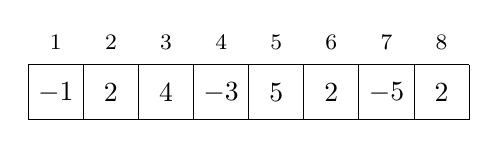
\begin{tikzpicture}[scale=0.7]
\draw (0,0) grid (8,1);

\node at (0.5,0.5) {$-1$};
\node at (1.5,0.5) {$2$};
\node at (2.5,0.5) {$4$};
\node at (3.5,0.5) {$-3$};
\node at (4.5,0.5) {$5$};
\node at (5.5,0.5) {$2$};
\node at (6.5,0.5) {$-5$};
\node at (7.5,0.5) {$2$};

\footnotesize
\node at (0.5,1.4) {$1$};
\node at (1.5,1.4) {$2$};
\node at (2.5,1.4) {$3$};
\node at (3.5,1.4) {$4$};
\node at (4.5,1.4) {$5$};
\node at (5.5,1.4) {$6$};
\node at (6.5,1.4) {$7$};
\node at (7.5,1.4) {$8$};
\end{tikzpicture}
\end{center}

optimiratkaisu on valita alitaulukko seuraavasti:

\begin{center}
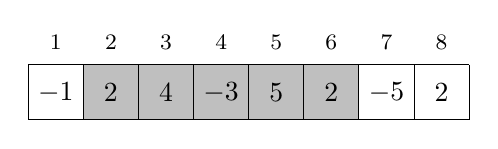
\begin{tikzpicture}[scale=0.7]
\fill[color=lightgray] (1,0) rectangle (6,1);
\draw (0,0) grid (8,1);

\node at (0.5,0.5) {$-1$};
\node at (1.5,0.5) {$2$};
\node at (2.5,0.5) {$4$};
\node at (3.5,0.5) {$-3$};
\node at (4.5,0.5) {$5$};
\node at (5.5,0.5) {$2$};
\node at (6.5,0.5) {$-5$};
\node at (7.5,0.5) {$2$};

\footnotesize
\node at (0.5,1.4) {$1$};
\node at (1.5,1.4) {$2$};
\node at (2.5,1.4) {$3$};
\node at (3.5,1.4) {$4$};
\node at (4.5,1.4) {$5$};
\node at (5.5,1.4) {$6$};
\node at (6.5,1.4) {$7$};
\node at (7.5,1.4) {$8$};
\end{tikzpicture}
\end{center}

Tämän alitaulukon lukujen summa on $2+4+(-3)+5+2=10$,
joka on suurin mahdollinen.
Keskellä oleva negatiivinen luku $-3$ kannattaa
ottaa mukaan, koska sen kummallakin puolella olevat
luvut kasvattavat summaa yli $3$:lla.

\subsubsection{Ratkaisu 1 ($O(n^3)$)}

Suoraviivainen ratkaisu tehtävään on käydä
läpi kaikki tavat valita alitaulukko taulukosta,
laskea jokaisesta vaihtoehdosta lukujen summa
ja pitää muistissa suurinta summaa.
Seuraava koodi toteuttaa tämän algoritmin:

\begin{lstlisting}
int p = 0;
for (int a = 1; a <= n; a++) {
    for (int b = a; b <= n; b++) {
        int s = 0;
        for (int c = a; c <= b; c++) {
            s += t[c];
        }
        p = max(p,s);
    }
}
cout << p << "\n";
\end{lstlisting}

Koodi olettaa, että luvut on tallennettu taulukkoon \texttt{t},
jota indeksoidaan $1 \ldots n$.
Muuttujat $a$ ja $b$ valitsevat alitaulukon ensimmäisen
ja viimeisen luvun, ja alitaulukon summa lasketaan muuttujaan $s$.
Muuttujassa $p$ on taas paras haun aikana löydetty summa.

Algoritmin aikavaativuus on $O(n^3)$, koska siinä on kolme
sisäkkäistä silmukkaa ja jokainen silmukka käy läpi $O(n)$ lukua.

\subsubsection{Ratkaisu 2 ($O(n^2)$)}

Äskeistä ratkaisua on helppoa tehostaa hankkiutumalla
eroon sisimmästä silmukasta.
Tämä on mahdollista laskemalla summaa samalla,
kun alitaulukon oikea reuna liikkuu eteenpäin.
Tuloksena on seuraava koodi:

\begin{lstlisting}
int p = 0;
for (int a = 1; a <= n; a++) {
    int s = 0;
    for (int b = a; b <= n; b++) {
        s += t[b];
        p = max(p,s);
    }
}
cout << p << "\n";
\end{lstlisting}

Tämän muutoksen jälkeen koodin aikavaativuus on $O(n^2)$,
koska siinä on kaksi sisäkkäistä silmukkaa.

\subsubsection{Ratkaisu 3 ($O(n)$)}

Yllättävää kyllä, tehtävään on olemassa myös
$O(n)$-aikainen ratkaisu eli koodista pystyy
karsimaan vielä yhden silmukan.
Ratkaisun ideana on laskea taulukon jokaiseen
kohtaan, mikä on suurin mahdollinen summa
kyseiseen kohtaan päättyvässä alitaulukossa,
ja valita suurin näistä summista.

Kun alitaulukon loppukohta $k$ on valittu,
sen muodostamiseen on kaksi vaihtoehtoa.
Yksi mahdollisuus on, että alitaulukossa
on vain yksi luku: kohdassa $k$ oleva luku.
Muussa tapauksessa siinä on ensin
kohtaan $k-1$ päättyvä alitaulukko,
johon on yhdistetty kohdassa $k$ oleva luku.

Koska tavoitteena on saada aikaan mahdollisimman
suuri summa, jälkimmäisessä tapauksessa myös
kohtaan $k-1$ päättyvä alitaulukko tulee valita niin,
että sen summa on mahdollisimman suuri.
Niinpä tehokas ratkaisu syntyy käymällä läpi
kaikki loppukohdat $k$ järjestyksessä.

Seuraava koodi toteuttaa ratkaisun:

\begin{lstlisting}
int p = 0, s = 0;
for (int k = 1; k <= n; k++) {
    s = max(t[k],s+t[k]);
    p = max(p,s);
}
cout << p << "\n";
\end{lstlisting}

Algoritmissa on vain yksi silmukka,
joka käy läpi taulukon luvut,
joten sen aikavaativuus on $O(n)$.
Tämä on myös paras mahdollinen aikavaativuus,
koska minkä tahansa algoritmin täytyy käydä
läpi ainakin kerran taulukon sisältö.

\subsubsection{Tehokkuusvertailu}

On kiinnostavaa tutkia, kuinka tehokkaita algoritmit
ovat käytännössä.
Seuraava taulukko näyttää, kuinka nopeasti äskeiset
ratkaisut toimivat eri $n$:n arvoilla
(testikoneena Intel Core i7-2677M, 1{,}80 GHz).

Jokainen syöte on muodostettu satunnaisesti,
ja taulukon luvut ovat välillä $-10^9 \ldots 10^9$.
Ajankäyttöön ei ole laskettu syötteen lukemiseen
kuluvaa aikaa.

\begin{center}
\begin{tabular}{rrrr}
taulukon koko $n$ & ratkaisu 1 & ratkaisu 2 & ratkaisu 3 \\
\hline
$10^2$ & $0{,}0$ s & $0{,}0$ s & $0{,}0$ s \\
$10^3$ & $0{,}1$ s & $0{,}0$ s & $0{,}0$ s \\
$10^4$ & > $10,0$ s & $0{,}1$ s & $0{,}0$ s \\
$10^5$ & > $10,0$ s & $5{,}3$ s & $0{,}0$ s \\
$10^6$ & > $10,0$ s & > $10,0$ s & $0{,}0$ s \\
$10^7$ & > $10,0$ s & > $10,0$ s & $0{,}0$ s \\
\end{tabular}
\end{center}

Vertailu osoittaa,
että pienillä syötteillä kaikki algoritmit
ovat tehokkaita,
mutta suuremmat syötteet tuovat esille
huomattavia eroja algoritmien suoritusajassa.
$O(n)$-aikainen ratkaisu 3 on ainoa,
joka pystyy ratkaisemaan kaikki syötteet
alle 10 sekunnissa.
\chapter{Järjestäminen}

\index{jxrjestxminen@järjestäminen}

\key{Järjestäminen} (''sorting'')
on keskeinen algoritmiikan ongelma.
Moni tehokas algoritmi
perustuu järjestämiseen,
koska järjestetyn tiedon
käsittely on helpompaa
kuin sekalaisessa järjestyksessä olevan.

Esimerkiksi kysymys ''onko taulukossa kahta samaa
alkiota?'' ratkeaa tehokkaasti järjestämisen avulla.
Jos taulukossa on kaksi samaa alkiota,
ne ovat järjestämisen jälkeen peräkkäin,
jolloin niiden löytäminen on helppoa.
Samaan tapaan ratkeaa myös kysymys
''mikä on yleisin alkio taulukossa?''.

Järjestämiseen on kehitetty monia
algoritmeja, jotka tarjoavat hyviä
esimerkkejä algoritmien suunnittelun tekniikoista.
Tehokkaat yleiset järjestämis\-algoritmit
toimivat ajassa $O(n \log n)$, ja tämä aikavaativuus
on myös monella järjestämistä käyttävällä algoritmilla.

\section{Järjestämisen teoriaa}

Järjestämisen perusongelma on seuraava:

\begin{task}
Annettuna on taulukko, jossa on $n$ alkiota.
Tehtäväsi on järjestää alkiot pienimmästä
suurimpaan.
\end{task}

Esimerkiksi taulukko
\begin{center}
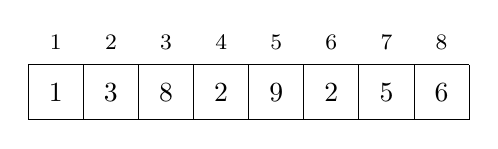
\begin{tikzpicture}[scale=0.7]
\draw (0,0) grid (8,1);
\node at (0.5,0.5) {$1$};
\node at (1.5,0.5) {$3$};
\node at (2.5,0.5) {$8$};
\node at (3.5,0.5) {$2$};
\node at (4.5,0.5) {$9$};
\node at (5.5,0.5) {$2$};
\node at (6.5,0.5) {$5$};
\node at (7.5,0.5) {$6$};

\footnotesize
\node at (0.5,1.4) {$1$};
\node at (1.5,1.4) {$2$};
\node at (2.5,1.4) {$3$};
\node at (3.5,1.4) {$4$};
\node at (4.5,1.4) {$5$};
\node at (5.5,1.4) {$6$};
\node at (6.5,1.4) {$7$};
\node at (7.5,1.4) {$8$};
\end{tikzpicture}
\end{center}
on järjestettynä seuraava:
\begin{center}
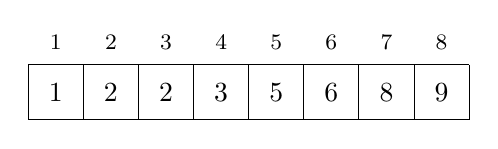
\begin{tikzpicture}[scale=0.7]
\draw (0,0) grid (8,1);
\node at (0.5,0.5) {$1$};
\node at (1.5,0.5) {$2$};
\node at (2.5,0.5) {$2$};
\node at (3.5,0.5) {$3$};
\node at (4.5,0.5) {$5$};
\node at (5.5,0.5) {$6$};
\node at (6.5,0.5) {$8$};
\node at (7.5,0.5) {$9$};

\footnotesize
\node at (0.5,1.4) {$1$};
\node at (1.5,1.4) {$2$};
\node at (2.5,1.4) {$3$};
\node at (3.5,1.4) {$4$};
\node at (4.5,1.4) {$5$};
\node at (5.5,1.4) {$6$};
\node at (6.5,1.4) {$7$};
\node at (7.5,1.4) {$8$};
\end{tikzpicture}
\end{center}

\subsubsection{$O(n^2)$-algoritmit}

\index{kuplajxrjestxminen@kuplajärjestäminen}

Yksinkertaiset algoritmit taulukon
järjestämiseen vievät aikaa $O(n^2)$.
Ehkä tunnetuin tällainen algoritmi on
\key{kuplajärjestäminen} (''bubble sort''),
joka muodostuu peräkkäisistä taulukon läpikäynneistä.

Algoritmissa jokainen taulukon läpikäynti
etsii vierekkäisiä alkiopareja,
jotka ovat väärässä järjestyksessä,
ja korjaa näiden alkioparien järjestyksen.
Algoritmi päättyy, kun läpikäynnin
aikana ei tule mitään muutoksia taulukkoon,
jolloin taulukko on järjestyksessä.

Kuplajärjestämisen voi toteuttaa seuraavasti,
kun järjestettävä taulukko muodostuu alkioista
$\texttt{t}[1],\texttt{t}[2],\ldots,\texttt{t}[n]$:
\begin{lstlisting}
bool stop = false;
while (!stop) {
    stop = true;
    for (int i = 1; i <= n-1; i++) {
        if (t[i] > t[i+1]) {
            swap(t[i],t[i+1]);
            stop = false;
        }
    }
}
\end{lstlisting}

\noindent
Esimerkiksi taulukossa

\begin{center}
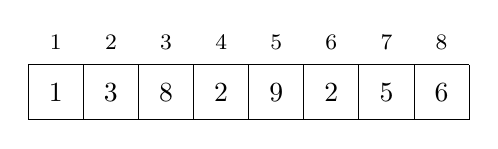
\begin{tikzpicture}[scale=0.7]
\draw (0,0) grid (8,1);

\node at (0.5,0.5) {$1$};
\node at (1.5,0.5) {$3$};
\node at (2.5,0.5) {$8$};
\node at (3.5,0.5) {$2$};
\node at (4.5,0.5) {$9$};
\node at (5.5,0.5) {$2$};
\node at (6.5,0.5) {$5$};
\node at (7.5,0.5) {$6$};

\footnotesize
\node at (0.5,1.4) {$1$};
\node at (1.5,1.4) {$2$};
\node at (2.5,1.4) {$3$};
\node at (3.5,1.4) {$4$};
\node at (4.5,1.4) {$5$};
\node at (5.5,1.4) {$6$};
\node at (6.5,1.4) {$7$};
\node at (7.5,1.4) {$8$};
\end{tikzpicture}
\end{center}

\noindent
kuplajärjestämisen ensimmäinen
läpikäynti tekee seuraavat vaihdot:

\begin{center}
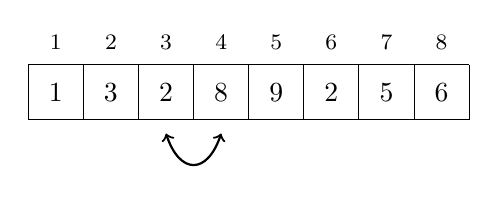
\begin{tikzpicture}[scale=0.7]
\draw (0,0) grid (8,1);
\node at (0.5,0.5) {$1$};
\node at (1.5,0.5) {$3$};
\node at (2.5,0.5) {$2$};
\node at (3.5,0.5) {$8$};
\node at (4.5,0.5) {$9$};
\node at (5.5,0.5) {$2$};
\node at (6.5,0.5) {$5$};
\node at (7.5,0.5) {$6$};

\draw[thick,<->] (3.5,-0.25) .. controls (3.25,-1.00) and (2.75,-1.00) .. (2.5,-0.25);

\footnotesize
\node at (0.5,1.4) {$1$};
\node at (1.5,1.4) {$2$};
\node at (2.5,1.4) {$3$};
\node at (3.5,1.4) {$4$};
\node at (4.5,1.4) {$5$};
\node at (5.5,1.4) {$6$};
\node at (6.5,1.4) {$7$};
\node at (7.5,1.4) {$8$};
\end{tikzpicture}
\end{center}

\begin{center}
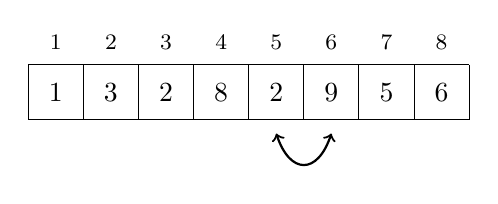
\begin{tikzpicture}[scale=0.7]
\draw (0,0) grid (8,1);
\node at (0.5,0.5) {$1$};
\node at (1.5,0.5) {$3$};
\node at (2.5,0.5) {$2$};
\node at (3.5,0.5) {$8$};
\node at (4.5,0.5) {$2$};
\node at (5.5,0.5) {$9$};
\node at (6.5,0.5) {$5$};
\node at (7.5,0.5) {$6$};

\draw[thick,<->] (5.5,-0.25) .. controls (5.25,-1.00) and (4.75,-1.00) .. (4.5,-0.25);


\footnotesize
\node at (0.5,1.4) {$1$};
\node at (1.5,1.4) {$2$};
\node at (2.5,1.4) {$3$};
\node at (3.5,1.4) {$4$};
\node at (4.5,1.4) {$5$};
\node at (5.5,1.4) {$6$};
\node at (6.5,1.4) {$7$};
\node at (7.5,1.4) {$8$};
\end{tikzpicture}
\end{center}

\begin{center}
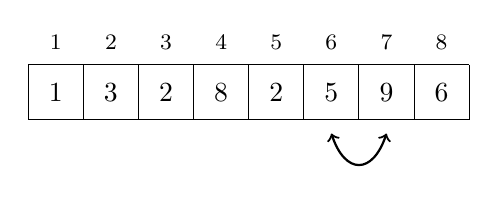
\begin{tikzpicture}[scale=0.7]
\draw (0,0) grid (8,1);
\node at (0.5,0.5) {$1$};
\node at (1.5,0.5) {$3$};
\node at (2.5,0.5) {$2$};
\node at (3.5,0.5) {$8$};
\node at (4.5,0.5) {$2$};
\node at (5.5,0.5) {$5$};
\node at (6.5,0.5) {$9$};
\node at (7.5,0.5) {$6$};

\draw[thick,<->] (6.5,-0.25) .. controls (6.25,-1.00) and (5.75,-1.00) .. (5.5,-0.25);


\footnotesize
\node at (0.5,1.4) {$1$};
\node at (1.5,1.4) {$2$};
\node at (2.5,1.4) {$3$};
\node at (3.5,1.4) {$4$};
\node at (4.5,1.4) {$5$};
\node at (5.5,1.4) {$6$};
\node at (6.5,1.4) {$7$};
\node at (7.5,1.4) {$8$};
\end{tikzpicture}
\end{center}

\begin{center}
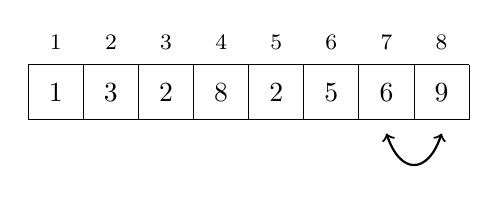
\begin{tikzpicture}[scale=0.7]
\draw (0,0) grid (8,1);
\node at (0.5,0.5) {$1$};
\node at (1.5,0.5) {$3$};
\node at (2.5,0.5) {$2$};
\node at (3.5,0.5) {$8$};
\node at (4.5,0.5) {$2$};
\node at (5.5,0.5) {$5$};
\node at (6.5,0.5) {$6$};
\node at (7.5,0.5) {$9$};

\draw[thick,<->] (7.5,-0.25) .. controls (7.25,-1.00) and (6.75,-1.00) .. (6.5,-0.25);

\footnotesize
\node at (0.5,1.4) {$1$};
\node at (1.5,1.4) {$2$};
\node at (2.5,1.4) {$3$};
\node at (3.5,1.4) {$4$};
\node at (4.5,1.4) {$5$};
\node at (5.5,1.4) {$6$};
\node at (6.5,1.4) {$7$};
\node at (7.5,1.4) {$8$};
\end{tikzpicture}
\end{center}


Kuplajärjestämisessä ensimmäisen läpikäynnin jälkeen suurin alkio
on paikallaan, toisen läpikäynnin jälkeen
kaksi suurinta alkiota on paikallaan, jne.
Niinpä kuplajärjestäminen päättyy aina viimeistään $n$
läpikäynnin jälkeen.
Koska jokainen läpikäynti vie aikaa $O(n)$,
algoritmin aikavaativuus on $O(n^2)$.

\subsubsection{Inversiot}

\index{inversio@inversio}

Kuplajärjestäminen on esimerkki algoritmista,
joka perustuu taulukon vierekkäisten alkioiden
vaihtamiseen.
Osoittautuu, että minkään tällaisen algoritmin
aikavaativuus ei voi olla parempi kuin $O(n^2)$,
koska tarvittava vaihtojen määrä
saattaa olla luokkaa $O(n^2)$.

Hyödyllinen käsite järjestämisalgoritmien
analyysissa on \key{inversio}.
Se on indeksipari $(a,b)$, joille $a<b$
ja $\texttt{t}[a]>\texttt{t}[b]$
eli kaksi taulukon alkiota, jotka ovat väärässä
järjestyksessä.
Esimerkiksi taulukon
\begin{center}
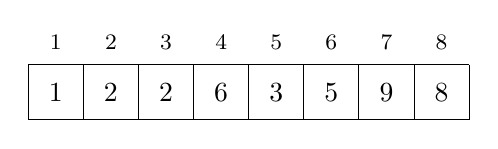
\begin{tikzpicture}[scale=0.7]
\draw (0,0) grid (8,1);
\node at (0.5,0.5) {$1$};
\node at (1.5,0.5) {$2$};
\node at (2.5,0.5) {$2$};
\node at (3.5,0.5) {$6$};
\node at (4.5,0.5) {$3$};
\node at (5.5,0.5) {$5$};
\node at (6.5,0.5) {$9$};
\node at (7.5,0.5) {$8$};

\footnotesize
\node at (0.5,1.4) {$1$};
\node at (1.5,1.4) {$2$};
\node at (2.5,1.4) {$3$};
\node at (3.5,1.4) {$4$};
\node at (4.5,1.4) {$5$};
\node at (5.5,1.4) {$6$};
\node at (6.5,1.4) {$7$};
\node at (7.5,1.4) {$8$};
\end{tikzpicture}
\end{center}
inversiot ovat $(4,5)$, $(4,6)$ ja $(7,8)$.
Inversioiden määrä kuvaa, miten lähellä
järjestystä taulukko on.
Järjestetyn taulukon inversioiden määrä on 0,
ja käänteisesti järjestetyn taulukon
inversioiden määrä on $1+2+\cdots+(n-1)=\frac{n(n-1)}{2}$.

Jos vierekkäiset alkiot ovat väärässä järjestyksessä,
niiden vaihtaminen keskenään poistaa
taulukosta yhden inversion.
Niinpä inversioiden määrä on sama kuin
taulukon järjestämiseen tarvittava vaihtojen määrä.
Vierekkäisiä alkioita
vaihtavan algoritmin aikavaativuus
on aina ainakin $O(n^2)$,
koska sen täytyy tehdä pahimmassa tapauksessa
$\frac{n(n-1)}{2} = O(n^2)$ vaihtoa.

\subsubsection{$O(n \log n)$-algoritmit}

\index{lomitusjxrjestxminen@lomitusjärjestäminen}

Tehokkaat järjestämisalgoritmit vievät
aikaa $O(n \log n)$.
Yksi tällainen algoritmi on
\key{lomitusjärjestäminen} (''merge sort''),
joka järjestää taulukon
rekursiivisesti jakamalla sen
pienemmiksi osataulukoiksi.

Lomitusjärjestäminen
jakaa taulukon kahdeksi osataulukoksi,
järjestää osataulukot rekursiivisesti ja muodostaa
sitten järjestetyn taulukon yhdistämällä osataulukot.
Algoritmin runko on seuraava:
\begin{lstlisting}
void mergesort(int a, int b) {
    if (a == b) return;
    int c = (a+b)/2;
    mergesort(a,c);
    mergesort(c+1,b);
    merge(a,c,c+1,b);
}
\end{lstlisting}

Funktio \texttt{mergesort}
järjestää taulukon välin $a \ldots b$ alkiot.
Jos $a=b$, välillä on vain yksi alkio,
joten se on valmiiksi järjestyksessä.
Muuten algoritmi jakaa välin
kahteen osaan: vasen osa on väli $a \ldots c$
ja oikea osa on väli $c+1 \ldots b$, missä $c=(a+b)/2$.
Algoritmi järjestää osat rekursiivisesti
kutsumalla itseään.

Algoritmi kutsuu funktiota \texttt{merge},
joka lomittaa välin vasemman ja oikean osan alkiot.
Tämä tarkoittaa, että alkiot kerätään yhteen niin,
että koko taulukon väli on järjestyksessä.
Lomitus
on mahdollista toteuttaa ajassa $O(n)$
valitsemalla alkiot järjestyksessä vasemman ja
oikean osan alusta alkaen.

\begin{samepage}
Esimerkiksi taulukko
\begin{center}
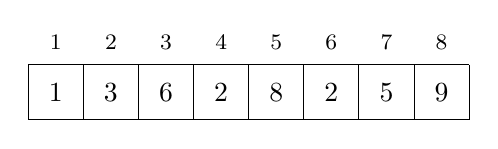
\begin{tikzpicture}[scale=0.7]
\draw (0,0) grid (8,1);
\node at (0.5,0.5) {$1$};
\node at (1.5,0.5) {$3$};
\node at (2.5,0.5) {$6$};
\node at (3.5,0.5) {$2$};
\node at (4.5,0.5) {$8$};
\node at (5.5,0.5) {$2$};
\node at (6.5,0.5) {$5$};
\node at (7.5,0.5) {$9$};

\footnotesize
\node at (0.5,1.4) {$1$};
\node at (1.5,1.4) {$2$};
\node at (2.5,1.4) {$3$};
\node at (3.5,1.4) {$4$};
\node at (4.5,1.4) {$5$};
\node at (5.5,1.4) {$6$};
\node at (6.5,1.4) {$7$};
\node at (7.5,1.4) {$8$};
\end{tikzpicture}
\end{center}
\end{samepage}
jakautuu osataulukoiksi
\begin{center}
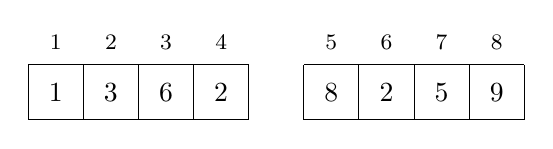
\begin{tikzpicture}[scale=0.7]
\draw (0,0) grid (4,1);
\draw (5,0) grid (9,1);

\node at (0.5,0.5) {$1$};
\node at (1.5,0.5) {$3$};
\node at (2.5,0.5) {$6$};
\node at (3.5,0.5) {$2$};

\node at (5.5,0.5) {$8$};
\node at (6.5,0.5) {$2$};
\node at (7.5,0.5) {$5$};
\node at (8.5,0.5) {$9$};

\footnotesize
\node at (0.5,1.4) {$1$};
\node at (1.5,1.4) {$2$};
\node at (2.5,1.4) {$3$};
\node at (3.5,1.4) {$4$};
\node at (5.5,1.4) {$5$};
\node at (6.5,1.4) {$6$};
\node at (7.5,1.4) {$7$};
\node at (8.5,1.4) {$8$};

\end{tikzpicture}
\end{center}
jotka ovat järjestettyinä
\begin{center}
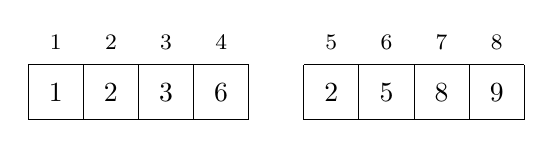
\begin{tikzpicture}[scale=0.7]
\draw (0,0) grid (4,1);
\draw (5,0) grid (9,1);

\node at (0.5,0.5) {$1$};
\node at (1.5,0.5) {$2$};
\node at (2.5,0.5) {$3$};
\node at (3.5,0.5) {$6$};

\node at (5.5,0.5) {$2$};
\node at (6.5,0.5) {$5$};
\node at (7.5,0.5) {$8$};
\node at (8.5,0.5) {$9$};

\footnotesize
\node at (0.5,1.4) {$1$};
\node at (1.5,1.4) {$2$};
\node at (2.5,1.4) {$3$};
\node at (3.5,1.4) {$4$};
\node at (5.5,1.4) {$5$};
\node at (6.5,1.4) {$6$};
\node at (7.5,1.4) {$7$};
\node at (8.5,1.4) {$8$};
\end{tikzpicture}
\end{center}
Osataulukot lomittamalla syntyy järjestetty taulukko
\begin{center}
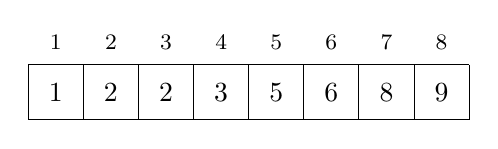
\begin{tikzpicture}[scale=0.7]
\draw (0,0) grid (8,1);
\node at (0.5,0.5) {$1$};
\node at (1.5,0.5) {$2$};
\node at (2.5,0.5) {$2$};
\node at (3.5,0.5) {$3$};
\node at (4.5,0.5) {$5$};
\node at (5.5,0.5) {$6$};
\node at (6.5,0.5) {$8$};
\node at (7.5,0.5) {$9$};

\footnotesize
\node at (0.5,1.4) {$1$};
\node at (1.5,1.4) {$2$};
\node at (2.5,1.4) {$3$};
\node at (3.5,1.4) {$4$};
\node at (4.5,1.4) {$5$};
\node at (5.5,1.4) {$6$};
\node at (6.5,1.4) {$7$};
\node at (7.5,1.4) {$8$};
\end{tikzpicture}
\end{center}

Lomitusjärjestämisen aikavaativuus on $O(n \log n)$,
koska algoritmin aikana
osataulukoista muodostuu $O(\log n)$ tasoa
ja kullakin tasolla osataulukoiden lomitus
vie yhteensä $O(n)$ aikaa.

\subsubsection{Järjestämisen alaraja}

Monet järjestämisalgoritmi saavuttavat
aikavaativuuden $O(n \log n)$,
mutta kukaan ei ole onnistunut keksimään
yleistä järjestämisalgoritmia,
joka toimisi nopeammin kuin $O(n \log n)$.
Tähän on yllättävä syy: on mahdollista todistaa,
että tällaista algoritmia ei ole olemassa.

Ideana todistuksessa on tarkastella järjestämistä
prosessina, jossa jokainen kahden alkion vertailu
antaa lisää tietoa taulukon sisällöstä.
Prosessista muodostuu seuraavanlainen puu:

\begin{center}
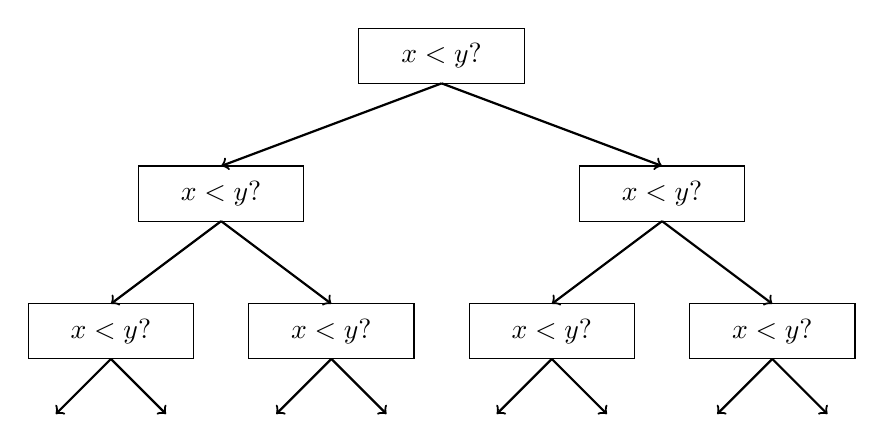
\begin{tikzpicture}[scale=0.7]
\draw (0,0) rectangle (3,1);
\node at (1.5,0.5) {$x < y?$};

\draw[thick,->] (1.5,0) -- (-2.5,-1.5);
\draw[thick,->] (1.5,0) -- (5.5,-1.5);

\draw (-4,-2.5) rectangle (-1,-1.5);
\draw (4,-2.5) rectangle (7,-1.5);
\node at (-2.5,-2) {$x < y?$};
\node at (5.5,-2) {$x < y?$};

\draw[thick,->] (-2.5,-2.5) -- (-4.5,-4);
\draw[thick,->] (-2.5,-2.5) -- (-0.5,-4);
\draw[thick,->] (5.5,-2.5) -- (3.5,-4);
\draw[thick,->] (5.5,-2.5) -- (7.5,-4);

\draw (-6,-5) rectangle (-3,-4);
\draw (-2,-5) rectangle (1,-4);
\draw (2,-5) rectangle (5,-4);
\draw (6,-5) rectangle (9,-4);
\node at (-4.5,-4.5) {$x < y?$};
\node at (-0.5,-4.5) {$x < y?$};
\node at (3.5,-4.5) {$x < y?$};
\node at (7.5,-4.5) {$x < y?$};

\draw[thick,->] (-4.5,-5) -- (-5.5,-6);
\draw[thick,->] (-4.5,-5) -- (-3.5,-6);
\draw[thick,->] (-0.5,-5) -- (0.5,-6);
\draw[thick,->] (-0.5,-5) -- (-1.5,-6);
\draw[thick,->] (3.5,-5) -- (2.5,-6);
\draw[thick,->] (3.5,-5) -- (4.5,-6);
\draw[thick,->] (7.5,-5) -- (6.5,-6);
\draw[thick,->] (7.5,-5) -- (8.5,-6);
\end{tikzpicture}
\end{center}

Merkintä ''$x<y?$'' tarkoittaa taulukon alkioiden
$x$ ja $y$ vertailua.
Jos $x<y$, prosessi jatkaa vasemmalle,
ja muuten oikealle.
Prosessin tulokset ovat taulukon mahdolliset
järjestykset, joita on kaikkiaan $n!$ erilaista.
Puun korkeuden tulee olla tämän vuoksi vähintään

\[ \log_2(n!) = \log_2(1)+\log_2(2)+\cdots+\log_2(n) = O(n \log n).\]

\subsubsection{Laskemisjärjestäminen}

\index{laskemisjxrjestxminen@laskemisjärjestäminen}

Järjestämisen alaraja $O(n \log n)$ ei koske algoritmeja,
jotka eivät perustu alkioiden vertailuun vaan hyödyntävät
jotain muuta tietoa alkioista.
Esimerkki tällaisesta algoritmista on
\key{laskemisjärjestäminen}, joka järjestää
kokonaisluvuista koostuvan taulukon $O(n)$-ajassa.

Algoritmin ideana on luoda \emph{kirjanpito}, josta selviää,
montako kertaa mikäkin alkio esiintyy taulukossa.
Kirjanpito on taulukko, jonka indeksit ovat alkuperäisen
taulukon alkioita.
Jokaisen indeksin kohdalla lukee, montako kertaa
kyseinen alkio esiintyy alkuperäisessä taulukossa.

Esimerkiksi taulukosta
\begin{center}
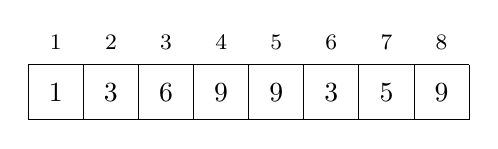
\begin{tikzpicture}[scale=0.7]
\draw (0,0) grid (8,1);
\node at (0.5,0.5) {$1$};
\node at (1.5,0.5) {$3$};
\node at (2.5,0.5) {$6$};
\node at (3.5,0.5) {$9$};
\node at (4.5,0.5) {$9$};
\node at (5.5,0.5) {$3$};
\node at (6.5,0.5) {$5$};
\node at (7.5,0.5) {$9$};

\footnotesize
\node at (0.5,1.4) {$1$};
\node at (1.5,1.4) {$2$};
\node at (2.5,1.4) {$3$};
\node at (3.5,1.4) {$4$};
\node at (4.5,1.4) {$5$};
\node at (5.5,1.4) {$6$};
\node at (6.5,1.4) {$7$};
\node at (7.5,1.4) {$8$};
\end{tikzpicture}
\end{center}
syntyy seuraava kirjanpito:
\begin{center}
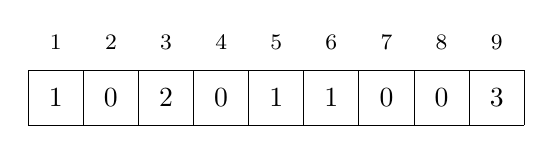
\begin{tikzpicture}[scale=0.7]
\draw (0,0) grid (9,1);
\node at (0.5,0.5) {$1$};
\node at (1.5,0.5) {$0$};
\node at (2.5,0.5) {$2$};
\node at (3.5,0.5) {$0$};
\node at (4.5,0.5) {$1$};
\node at (5.5,0.5) {$1$};
\node at (6.5,0.5) {$0$};
\node at (7.5,0.5) {$0$};
\node at (8.5,0.5) {$3$};

\footnotesize

\node at (0.5,1.5) {$1$};
\node at (1.5,1.5) {$2$};
\node at (2.5,1.5) {$3$};
\node at (3.5,1.5) {$4$};
\node at (4.5,1.5) {$5$};
\node at (5.5,1.5) {$6$};
\node at (6.5,1.5) {$7$};
\node at (7.5,1.5) {$8$};
\node at (8.5,1.5) {$9$};
\end{tikzpicture}
\end{center}

Esimerkiksi kirjanpidossa lukee indeksin 3 kohdalla 2,
koska luku 3 esiintyy kahdesti alkuperäisessä
taulukossa (indekseissä 2 ja 6).

Kirjanpidon muodostus vie aikaa $O(n)$,
koska riittää käydä taulukko läpi kerran.
Tämän jälkeen järjestetyn taulukon luominen
vie myös aikaa $O(n)$, koska kunkin alkion
määrän saa selville suoraan kirjanpidosta.
Niinpä laskemisjärjestämisen
kokonaisaikavaativuus on $O(n)$.

Laskemisjärjestäminen on hyvin tehokas algoritmi,
mutta sen käyttäminen vaatii,
että taulukon sisältönä on niin pieniä
kokonaislukuja, että niitä voi käyttää
kirjanpidon taulukon indeksöinnissä.

\section{Järjestäminen C++:ssa}

\index{sort@\texttt{sort}}

C++:n standardikirjastossa on funktio \texttt{sort},
jonka avulla voi järjestää helposti taulukoita
ja muita tietorakenteita.
Tätä funktiota kannattaa käyttää yleensä aina
järjestämiseen algoritmeissa,
koska funktio on toteutettu tehokkaasti ja varmasti toimivasti.

Seuraava koodi järjestää vektorin \texttt{v}
luvut pienimmästä suurimpaan:
\begin{lstlisting}
vector<int> v = {4,2,5,3,5,8,3};
sort(v.begin(),v.end());
\end{lstlisting}
Järjestämisen jälkeen vektorin sisältö on
$\{2,3,3,4,5,5,8\}$.

Oletuksena järjestys tapahtuu pienimmästä suurimpaan,
mutta järjestyksen saa käänteiseksi näin:
\begin{lstlisting}
sort(v.rbegin(),v.rend());
\end{lstlisting}

Tavallisen taulukon voi järjestää seuraavasti:
\begin{lstlisting}
int n = 7; // taulukon koko
int t[] = {4,2,5,3,5,8,3};
sort(t,t+n);
\end{lstlisting}

Seuraava koodi järjestää merkkijonon \texttt{s}:
\begin{lstlisting}
string s = "apina";
sort(s.begin(), s.end());
\end{lstlisting}

Merkkijonon järjestäminen tarkoittaa,
että sen merkit järjestetään aakkosjärjestykseen.
Esimerkiksi merkkijono ''apina''
on järjestettynä ''aainp''.

\subsubsection{Vertailuoperaattori}

\index{vertailuoperaattori@vertailuoperaattori}

Funktion \texttt{sort} käyttäminen vaatii,
että järjestettävien alkioiden
tietotyypille on määritelty \key{vertailuoperaattori} \texttt{<},
jonka avulla voi selvittää, mikä on kahden alkion järjestys.
Järjestämisen aikana \texttt{sort}-funktio
käyttää operaattoria \texttt{<} aina, kun sen täytyy
vertailla järjestettäviä alkioita.

Vertailuoperaattori on määritelty valmiiksi
useimmille C++:n tietotyypeille,
minkä ansiosta niitä pystyy järjestämään automaattisesti.
Jos järjestettävänä on lukuja, ne järjestyvät
suuruusjärjestykseen,
ja jos järjestettävänä on merkkijonoja,
ne järjestyvät aakkosjärjestykseen.

\index{pair@\texttt{pair}}

Parit (\texttt{pair}) järjestyvät ensisijaisesti
ensimmäisen kentän (\texttt{first}) mukaan.
Jos kuitenkin parien ensimmäiset kentät ovat samat,
järjestys määräytyy toisen kentän (\texttt{second}) mukaan.
Seuraava koodi esittelee asiaa:

\begin{lstlisting}
vector<pair<int,int>> v;
v.push_back({1,5});
v.push_back({2,3});
v.push_back({1,2});
sort(v.begin(), v.end());
\end{lstlisting}

Koodin suorituksen jälkeen parien järjestys on
$(1,2)$, $(1,5)$, $(2,3)$.

\index{tuple@\texttt{tuple}}
Vastaavasti \texttt{tuple}-rakenteet
järjestyvät ensisijaisesti ensimmäisen kentän,
toissijaisesti toisen kentän, jne., mukaan.
Seuraava koodi esittelee asiaa:
\begin{lstlisting}
vector<tuple<int,int,int>> v;
v.push_back(make_tuple(2,1,4));
v.push_back(make_tuple(1,5,3));
v.push_back(make_tuple(2,1,3));
sort(v.begin(),v.end());
\end{lstlisting}
Koodin suorituksen jälkeen järjestys on
$(1,5,3)$, $(2,1,3)$, $(2,1,4)$.

\subsubsection{Omat tietueet}

Jos järjestettävänä on omia tietueita,
niiden vertailuoperaattori täytyy toteuttaa itse.
Operaattori määritellään tietueen sisään
\texttt{operator<}-nimisenä funktiona,
jonka parametrina on toinen alkio.
Operaattorin tulee palauttaa \texttt{true},
jos oma alkio on pienempi kuin parametrialkio,
ja muuten \texttt{false}.

Esimerkiksi seuraava tietue \texttt{P}
sisältää pisteen x- ja y-koordinaatit.
Vertailuoperaattori on toteutettu niin,
että pisteet järjestyvät ensisijaisesti x-koor\-di\-naa\-tin
ja toissijaisesti y-koordinaatin mukaan.

\begin{lstlisting}
struct P {
    int x, y;
    bool operator<(const p& a) {
        if (this.x != a.x) return this.x < a.x;
        else return this.y < a.y;
    }
};
\end{lstlisting}

\subsubsection{Vertailufunktio}

\index{vertailufunktio@vertailufunktio}

On myös mahdollista antaa
\texttt{sort}-funktiolle ulkopuolinen \key{vertailufunktio}.
Esimerkiksi seuraava vertailufunktio
järjestää merkkijonot ensisijaisesti pituuden mukaan
ja toissijaisesti aakkosjärjestyksen mukaan:

\begin{lstlisting}
bool cmp(string a, string b) {
    if (a.size() != b.size()) return a.size() < b.size();
    return a < b;
}
\end{lstlisting}
Tämän jälkeen merkkijonovektorin voi järjestää näin:
\begin{lstlisting}
sort(v.begin(), v.end(), cmp);
\end{lstlisting}

\section{Binäärihaku}

\index{binxxrihaku@binäärihaku}

Tavallinen tapa etsiä alkiota $x$ taulukosta \texttt{t}
on käyttää \texttt{for}-silmukkaa, joka käy läpi
taulukon sisällön:

\begin{lstlisting}
for (int i = 1; i <= n; i++) {
    if (t[i] == x) // alkio x löytyi kohdasta i
}
\end{lstlisting}

Tämän menetelmän aikavaativuus on $O(n)$,
koska pahimmassa tapauksessa koko taulukko täytyy
käydä läpi.
Jos taulukon sisältö voi olla mitä tahansa,
tämä on kuitenkin tehokkain mahdollinen menetelmä,
koska saatavilla ei ole lisätietoa siitä,
mistä päin taulukkoa alkiota $x$ kannattaa etsiä.

Tilanne on toinen silloin, kun taulukko on
järjestyksessä.
Tässä tapauksessa haku on mahdollista toteuttaa
paljon nopeammin, koska alkioiden järjestys
ohjaa etsimään alkiota oikeasta suunnasta.
Seuraavaksi käsiteltävä \key{binäärihaku}
löytää alkion järjestetystä taulukosta
tehokkaasti ajassa $O(\log n)$.

\subsubsection{Toteutus 1}

Perinteinen tapa toteuttaa binäärihaku muistuttaa sanan etsimistä
sanakirjasta. Haku puolittaa joka askeleella hakualueen taulukossa,
kunnes lopulta etsittävä alkio löytyy tai osoittautuu,
että sitä ei ole taulukossa.

Haku tarkistaa ensin taulukon keskimmäisen alkion.
Jos keskimmäinen alkio on etsittävä alkio, haku päättyy.
Muuten haku jatkuu taulukon vasempaan tai oikeaan osaan sen mukaan,
onko keskimmäinen alkio suurempi vain pienempi kuin etsittävä alkio.

Yllä olevan idean voi toteuttaa seuraavasti:
\begin{lstlisting}
int a = 1, b = n;
while (a <= b) {
    int k = (a+b)/2;
    if (t[k] == x) // alkio x löytyi kohdasta k
    if (t[k] > x) b = k-1;
    else a = k+1;
}
\end{lstlisting}

Algoritmi pitää yllä väliä $a \ldots b$, joka on
jäljellä oleva hakualue taulukossa.
Aluksi väli on $1 \ldots n$ eli koko taulukko.
Välin koko puolittuu algoritmin joka vaiheessa,
joten aikavaativuus on $O(\log n)$.

\subsubsection{Toteutus 2}

Vaihtoehtoinen tapa toteuttaa binäärihaku
perustuu taulukon tehostettuun läpikäyntiin.
Ideana on käydä taulukkoa läpi hyppien
ja hidastaa vauhtia, kun etsittävä alkio lähestyy.

Haku käy taulukkoa läpi vasemmalta oikealle aloittaen
hypyn pituudesta $n$.
Joka vaiheessa hypyn pituus puolittuu:
ensin $n/2$, sitten $n/4$, sitten $n/8$ jne.,
kunnes lopulta hypyn pituus on 1.
Hyppyjen jälkeen joko haettava alkio on löytynyt
tai selviää, että sitä ei ole taulukossa.

Seuraava koodi toteuttaa äskeisen idean:
\begin{lstlisting}
int k = 1;
for (int b = n; b >= 1; b /= 2) {
    while (k+b <= n && t[k+b] <= x) k += b;
}
if (t[k] == x) // alkio x löytyi kohdasta k
\end{lstlisting}

Muuttuja $k$ on läpikäynnin kohta taulukossa
ja muuttuja $b$ on hypyn pituus.
Jos alkio $x$ esiintyy taulukossa,
sen kohta on muuttujassa $k$ algoritmin päätteeksi.
Algoritmin aikavaativuus on $O(\log n)$,
koska \texttt{while}-silmukassa oleva koodi suoritetaan
aina enintään kahdesti.

\subsubsection{Muutoskohdan etsiminen}

Käytännössä binäärihakua tarvitsee koodata
harvoin alkion etsimiseen taulukosta,
koska sen sijasta voi käyttää standardikirjastoa.
Esimerkiksi C++:n funktiot \texttt{lower\_bound}
ja \texttt{upper\_bound} toteuttavat binäärihaun
ja tietorakenne \texttt{set} ylläpitää joukkoa,
jonka operaatiot ovat $O(\log n)$-aikaisia.

Sitäkin tärkeämpi binäärihaun käyttökohde on 
funktion muutoskohdan etsiminen.
Oletetaan, että haluamme löytää pienimmän arvon $k$,
joka on kelvollinen ratkaisu ongelmaan.
Käytössämme on funktio $\texttt{ok}(x)$,
joka palauttaa \texttt{true}, jos $x$ on kelvollinen
ratkaisu, ja muuten \texttt{false}.
Lisäksi tiedämme, että $\texttt{ok}(x)$ on \texttt{false}
aina kun $x<k$ ja \texttt{true} aina kun $x \geq k$.

Toisin sanoen haluamme löytää funktion \texttt{ok} muutoskohdan,
jossa arvosta \texttt{false} tulee arvo \texttt{true}.
Tilanne näyttää seuraavalta:

\begin{center}
\begin{tabular}{r|rrrrrrrr}
$x$ & 0 & 1 & $\cdots$ & $k-1$ & $k$ & $k+1$ & $\cdots$ \\
\hline
$\texttt{ok}(x)$ & \texttt{false} & \texttt{false}
& $\cdots$ & \texttt{false} & \texttt{true} & \texttt{true} & $\cdots$ \\
\end{tabular}
\end{center}

\noindent
Nyt muutoskohta on mahdollista etsiä käyttämällä
binäärihakua:

\begin{lstlisting}
int x = -1;
for (int b = z; b >= 1; b /= 2) {
    while (!ok(x+b)) x += b;
}
int k = x+1;
\end{lstlisting}

Haku etsii suurimman $x$:n arvon,
jolla $\texttt{ok}(x)$ on \texttt{false}.
Niinpä tästä seuraava arvo $k=x+1$
on pienin arvo, jolla $\texttt{ok}(k)$ on \texttt{true}.
Hypyn aloituspituus $z$ tulee olla 
sopiva suuri luku, esimerkiksi sellainen,
jolla $\texttt{ok}(z)$ on varmasti \texttt{true}.

Algoritmi kutsuu $O(\log z)$ kertaa funktiota
\texttt{ok}, joten kokonaisaikavaativuus
riippuu siitä, kauanko funktion \texttt{ok}
suoritus kestää.
Esimerkiksi jos ratkaisun tarkastus
vie aikaa $O(n)$, niin kokonaisaikavaativuus
on $O(n \log z)$.

\subsubsection{Huippuarvon etsiminen}

Binäärihaulla voi myös etsiä
suurimman arvon funktiolle,
joka on ensin kasvava ja sitten laskeva.
Toisin sanoen tehtävänä on etsiä arvo
$k$ niin, että

\begin{itemize}
\item
$f(x)<f(x+1)$, kun $x<k$, ja
\item
$f(x)>f(x+1)$, kun $x >= k$.
\end{itemize}

Ideana on etsiä binäärihaulla
viimeinen kohta $x$,
jossa pätee $f(x)<f(x+1)$.
Tällöin $k=x+1$,
koska pätee $f(x+1)>f(x+2)$.
Seuraava koodi toteuttaa haun: 

\begin{lstlisting}
int x = -1;
for (int b = z; b >= 1; b /= 2) {
    while (f(x+b) < f(x+b+1)) x += b;
}
int k = x+1;
\end{lstlisting}

Huomaa, että toisin kuin tavallisessa binäärihaussa,
tässä ei ole sallittua,
että peräkkäiset arvot olisivat yhtä suuria.
Silloin ei olisi mahdollista tietää,
mihin suuntaan hakua tulee jatkaa.




\chapter{Tietorakenteet}

\index{tietorakenne}

Tietorakenne (\textit{data structure})
on tapa säilyttää tietoa tietokoneen muistissa.
Sopivan tietorakenteen valinta on tärkeää,
koska kullakin rakenteella on omat
vahvuutensa ja heikkoutensa.
Tietorakenteen valinnassa oleellinen kysymys on,
mitkä operaatiot rakenne toteuttaa tehokkaasti.

Tämä luku esittelee keskeisimmät
C++:n standardikirjaston tietorakenteet.
Valmiita tietorakenteita kannattaa käyttää
aina kun mahdollista, 
koska se säästää paljon aikaa toteutuksessa.
Myöhemmin kirjassa tutustumme erikoisempiin
rakenteisiin, joita ei ole valmiina C++:ssa.

\section{Dynaaminen taulukko}

\index{vektori}
\index{\texttt{vector}}

Dynaaminen taulukko on taulukko,
jonka kokoa pystyy muuttamaan
ohjelman suorituksen aikana.
C++:n tavallisin dynaaminen taulukko
on vektori (\texttt{vector}).
Sitä voi käyttää hyvin samalla tavalla
kuin tavallista taulukkoa.

Seuraava koodi luo tyhjän vektorin
ja lisää siihen kolme lukua:

\begin{lstlisting}
vector<int> v;
v.push_back(3); // [3]
v.push_back(2); // [3,2]
v.push_back(5); // [3,2,5]
\end{lstlisting}

Tämän jälkeen vektorin sisältöä voi käsitellä taulukon tavoin:

\begin{lstlisting}
cout << v[0] << "\n"; // 3
cout << v[1] << "\n"; // 2
cout << v[2] << "\n"; // 5
\end{lstlisting}

Funktio \texttt{size} kertoo, montako alkiota vektorissa on.
Seuraava koodi tulostaa kaikki vektorin alkiot:

\begin{lstlisting}
for (int i = 0; i < v.size(); i++) {
    cout << v[i] << "\n";
}
\end{lstlisting}

\begin{samepage}
Vektorin voi käydä myös läpi lyhyemmin näin:

\begin{lstlisting}
for (auto x : v) {
    cout << x << "\n";
}
\end{lstlisting}
\end{samepage}

Funktio \texttt{back} hakee vektorin viimeisen alkion,
ja funktio \texttt{pop\_back} poistaa vektorin
viimeisen alkion:

\begin{lstlisting}
vector<int> v;
v.push_back(5);
v.push_back(2);
cout << v.back() << "\n"; // 2
v.pop_back();
cout << v.back() << "\n"; // 5
\end{lstlisting}

Vektorin sisällön voi antaa myös sen luonnissa:

\begin{lstlisting}
vector<int> v = {2, 4, 2, 5, 1};
\end{lstlisting}

Kolmas tapa luoda vektori on ilmoittaa
vektorin koko ja alkuarvo:

\begin{lstlisting}
// koko 10, alkuarvo 0
vector<int> v(10);
// koko 10, alkuarvo 5
vector<int> w(10, 5)
\end{lstlisting}

Vektori on toteutettu sisäisesti tavallisena taulukkona.
Jos vektorin koko kasvaa ja taulukko jää liian pieneksi,
varataan uusi suurempi taulukko, johon kopioidaan
vektorin sisältö.
Näin tapahtuu kuitenkin niin harvoin, että vektorin
funktion \texttt{push\_back} aikavaativuus on
keskimäärin $O(1)$.

\subsubsection{Merkkijono}

\index{merkkijono}
\index{\texttt{string}}

Myös merkkijono (\texttt{string}) on dynaaminen taulukko,
jota pystyy käsittelemään lähes samaan
tapaan kuin vektoria.
Merkkijonon käsittelyyn liittyy lisäksi erikoissyntaksia
ja funktioita, joita ei ole muissa tietorakenteissa.

Merkkijonoja voi yhdistää toisiinsa \texttt{+}-merkin avulla.
Funktio $\texttt{substr}(k,x)$ erottaa merkkijonosta
osajonon, joka alkaa kohdasta $k$ ja jonka pituus on $x$.
Funktio $\texttt{find}(\texttt{t})$ etsii kohdan,
jossa osajono \texttt{t} esiintyy merkkijonossa.

Seuraava koodi esittelee merkkijonon käyttämistä:

\begin{lstlisting}
string a = "hatti";
string b = a+a;
cout << b << "\n"; // hattihatti
b[5] = 'v';
cout << b << "\n"; // hattivatti
string c = b.substr(3,4);
cout << c << "\n"; // tiva
\end{lstlisting}

\section{Joukko}

\index{joukko}
\index{\texttt{set}}
\index{\texttt{unordered\_set}}


Joukko (\textit{set}) on tietorakenne,
joka muodostuu siinä olevista alkioista.
Joukon perusoperaatiot ovat alkion lisäys,
haku ja poisto.

C++ sisältää kaksi
toteutusta joukolle: \texttt{set} ja \texttt{unordered\_set}.
Rakenne \texttt{set} perustuu tasapainoiseen
binääripuuhun, ja sen operaatioiden aikavaativuus
on $O(\log n)$.
Rakenne \texttt{unordered\_set} pohjautuu hajautustauluun,
ja sen operaatioiden aikavaativuus on keskimäärin $O(1)$.

Usein on makuasia, kumpaa joukon toteutusta käyttää.
Rakenteen \texttt{set} etuna on, että se säilyttää
joukon alkioita järjestyksessä ja tarjoaa
järjestykseen liittyviä funktioita,
joita \texttt{unordered\_set} ei sisällä.
Toisaalta \texttt{unordered\_set} on usein hieman nopeampi
rakenne.

Seuraava koodi luo lukuja sisältävän joukon ja
esittelee sen käyttämistä.
Funktio \texttt{insert} lisää joukkoon alkion,
funktio \texttt{count} laskee alkion määrän joukossa
ja funktio \texttt{erase} poistaa alkion joukosta.

\begin{lstlisting}
set<int> s;
s.insert(3);
s.insert(2);
s.insert(5);
cout << s.count(3) << "\n"; // 1
cout << s.count(4) << "\n"; // 0
s.erase(3);
s.insert(4);
cout << s.count(3) << "\n"; // 0
cout << s.count(4) << "\n"; // 1
\end{lstlisting}

Tärkeä joukon ominaisuus on,
että tietty alkio voi esiintyä siinä
vain kerran.
Niinpä funktio \texttt{count} palauttaa aina
arvon 0 (alkiota ei ole joukossa) tai 1 (alkio on joukossa)
ja funktio \texttt{insert} ei lisää alkiota
uudestaan joukkoon, jos se on siellä valmiina.
Seuraava koodi havainnollistaa asiaa:

\begin{lstlisting}
set<int> s;
s.insert(5);
s.insert(5);
s.insert(5);
cout << s.count(5) << "\n"; // 1
\end{lstlisting}

\index{\texttt{multiset}}
\index{\texttt{unordered\_multiset}}

C++ sisältää myös rakenteet
\texttt{multiset} ja \texttt{unordered\_multiset},
jotka toimivat muuten samalla tavalla kuin \texttt{set}
ja \texttt{unordered\_set},
mutta sama alkio voi esiintyä
monta kertaa joukossa.
Esimerkiksi seuraavassa koodissa
kaikki luvun 5 kopiot lisätään joukkoon:

\begin{lstlisting}
multiset<int> s;
s.insert(5);
s.insert(5);
s.insert(5);
cout << s.count(5) << "\n"; // 3
\end{lstlisting}

Funktio \texttt{erase} poistaa
kaikki alkion esiintymät
\texttt{multiset}-rakenteessa:

\begin{lstlisting}
s.erase(5);
cout << s.count(5) << "\n"; // 0
\end{lstlisting}

Usein kuitenkin tulisi poistaa
vain yksi esiintymä,
mikä onnistuu näin:

\begin{lstlisting}
s.erase(s.find(5));
cout << s.count(5) << "\n"; // 2
\end{lstlisting}

\section{Hakemisto}

\index{hakemisto}
\index{\texttt{map}}
\index{\texttt{unordered\_map}}

Hakemisto (\textit{map}) on taulukon yleistys,
joka sisältää joukon avain-arvo-pareja.
Siinä missä taulukossa avaimet ovat aina peräkkäiset
kokonaisluvut $0,1,2,\ldots$,
hakemistossa ne voivat
olla mitä tahansa tyyppiä.

Joukkoa vastaavasti C++ sisältää sekä
binääripuuhun että hajautustauluun perustuvat
hakemistot \texttt{map} ja \texttt{unordered\_map},
joissa alkion käsittely vie aikaa vastaavasti
$O(\log n)$ ja keskimäärin $O(1)$.

Seuraava koodi toteuttaa hakemiston,
jossa avaimet ovat merkkijonoja ja
arvot ovat kokonaislukuja:

\begin{lstlisting}
map<string,int> m;
m["apina"] = 4;
m["banaani"] = 3;
m["cembalo"] = 9;
cout << m["banaani"] << "\n"; // 3
\end{lstlisting}

Jos hakemistosta hakee avainta,
jota ei ole siinä,
avain lisätään hakemistoon
automaattisesti oletusarvolla.
Esimerkiksi seuraavassa koodissa
hakemistoon ilmestyy avain ''aybabtu'',
jonka arvona on 0:

\begin{lstlisting}
map<string,int> m;
cout << m["aybabtu"] << "\n"; // 0
\end{lstlisting}

Komennolla \texttt{count} voi
tutkia, esiintyykö avain hakemistossa:

\begin{lstlisting}
if (m.count("aybabtu")) {
    cout << "avain on hakemistossa";
}
\end{lstlisting}

Seuraava koodi listaa hakemiston
kaikki avaimet ja arvot:

\begin{lstlisting}
for (auto x : m) {
    cout << x.first << " " << x.second << "\n";
}
\end{lstlisting}

\section{Iteraattorit ja välit}

\index{iteraattori}

Monet C++:n standardikirjaston funktiot
käsittelevät tietorakenteiden iteraattoreita
ja niiden määrittelemiä välejä.
Iteraattori (\textit{iterator}) on muuttuja,
joka osoittaa tiettyyn tietorakenteen alkioon.

Usein tarvittavat iteraattorit ovat \texttt{begin}
ja \texttt{end}, jotka rajaavat välin,
joka sisältää kaikki tietorakenteen alkiot.
Iteraattori \texttt{begin} osoittaa
tietorakenteen ensimmäiseen alkioon,
kun taas iteraattori \texttt{end} osoittaa
tietorakenteen viimeisen alkion jälkeiseen kohtaan.
Tilanne on siis tällainen:

\begin{center}
\begin{tabular}{llllllllll}
\{ & 3, & 4, & 6, & 8, & 12, & 13, & 14, & 17 & \} \\
& $\uparrow$ & & & & & & & & $\uparrow$ \\
& \multicolumn{3}{l}{\texttt{s.begin()}} & & & & & & \texttt{s.end()} \\
\end{tabular}
\end{center}

Huomaa epäsymmetria iteraattoreissa:
\texttt{s.begin()} osoittaa tietorakenteen alkioon,
kun taas \texttt{s.end()} osoittaa tietorakenteen ulkopuolelle.
Iteraattoreiden rajaama joukon väli on siis puoliavoin.

\subsubsection{Taulukon välit}

Iteraattoreita tarvitsee
C++:n standardikirjaston funktioissa, jotka käsittelevät
tietorakenteen välejä.
Yleensä halutaan käsitellä tietorakenteiden kaikkia
alkioita, jolloin funktiolle annetaan
iteraattorit \texttt{begin} ja \texttt{end}.

Seuraava koodi järjestää vektorin funktiolla \texttt{sort},
kääntää sitten alkioiden järjestyksen funktiolla \texttt{reverse}
ja sekoittaa lopuksi alkioiden järjestyksen funktiolla \texttt{random\_shuffle}.

\begin{lstlisting}
sort(v.begin(), v.end());
reverse(v.begin(), v.end());
random_shuffle(v.begin(), v.end());
\end{lstlisting}

Samoja funktioita voi myös käyttää tavallisen taulukon
yhteydessä, jolloin iteraattorin sijasta annetaan
osoitin taulukkoon:

\begin{lstlisting}
sort(t, t+n);
reverse(t, t+n);
random_shuffle(t, t+n);
\end{lstlisting}

\subsubsection{Joukon iteraattorit}

Iteraattoreita tarvitsee usein joukon
alkioiden käsittelyssä.
Seuraava koodi määrittelee iteraattorin
\texttt{it}, joka osoittaa joukon \texttt{s} alkuun:

\begin{lstlisting}
set<int>::iterator it = s.begin();
\end{lstlisting}

Koodin voi kirjoittaa myös lyhyemmin näin:

\begin{lstlisting}
auto it = s.begin();
\end{lstlisting}
Iteraattoria vastaavaan joukon alkioon
pääsee käsiksi \texttt{*}-merkinnällä.
Esimerkiksi seuraava koodi tulostaa
joukon ensimmäisen alkion:

\begin{lstlisting}
auto it = s.begin();
cout << *it << "\n";
\end{lstlisting}
Iteraattoria pystyy liikuttamaan
operaatioilla \texttt{++} (eteenpäin)
ja \texttt{---} (taaksepäin).
Tällöin iteraattori siirtyy seuraavaan
tai edelliseen alkioon joukossa.

Seuraava koodi tulostaa joukon kaikki alkiot:

\begin{lstlisting}
for (auto it = s.begin(); it != s.end(); it++) {
    cout << *it << "\n";
}
\end{lstlisting}
Seuraava koodi taas tulostaa joukon
viimeisen alkion:

\begin{lstlisting}
auto it = s.end();
it--;
cout << *it << "\n";
\end{lstlisting}
% Iteraattoria täytyi liikuttaa askel taaksepäin,
% koska se osoitti aluksi joukon viimeisen
% alkion jälkeiseen kohtaan.

Funktio \texttt{find} palauttaa iteraattorin
annettuun alkioon joukossa.
Mutta jos alkiota ei esiinny joukossa,
iteraattoriksi tulee \texttt{end}.

\begin{lstlisting}
auto it = s.find(x);
if (it == s.end()) cout << "x puuttuu joukosta";
\end{lstlisting}

Funktio $\texttt{lower\_bound}(x)$ palauttaa
iteraattorin joukon pienimpään alkioon,
joka on ainakin yhtä suuri kuin $x$.
Vastaavasti $\texttt{upper\_bound}(x)$ palauttaa
iteraattorin pienimpään alkioon,
joka on suurempi kuin $x$.
Jos tällaisia alkioita ei ole joukossa,
funktiot palauttavat arvon \texttt{end}.

Esimerkiksi seuraava koodi etsii joukosta
alkion, joka on lähinnä lukua $x$:

\begin{lstlisting}
auto a = s.lower_bound(x);
if (a == s.begin()) {
    cout << *a << "\n";
} else if (a == s.end()) {
    a--;
    cout << *a << "\n";
} else {
    auto b = a; b--;
    if (x-*b < *a-x) cout << *b << "\n";
    else cout << *a << "\n";
}
\end{lstlisting}
Iteraattori \texttt{a}
osoittaa pienimpään alkioon,
joka on ainakin yhtä suuri kuin $x$.
Jos tämä on joukon ensimmäinen alkio,
tämä on $x$:ää lähin alkio.
Jos tällaista alkiota ei ole,
$x$:ää lähin alkio on joukon viimeinen alkio.
Muussa tapauksessa $x$:ää lähin alkio
on joko $a$:n osoittama alkio tai tätä edellinen alkio.

\section{Muita tietorakenteita}

\subsubsection{Bittijoukko}

\index{bittijoukko}
\index{\texttt{bitset}}

Bittijoukko (\texttt{bitset}) on taulukko,
jonka jokaisen alkion arvo on 0 tai 1.
Bittijoukon etuna on, että jokainen alkio
vie vain yhden bitin tilaa muistissa.
Niinpä bittijoukon käyttäminen säästää muistia,
jos arvot 0 ja 1 riittävät.

Esimerkiksi jos taulukossa on $n$ arvoa
tallennettuna \texttt{int}-lukuina,
jokainen arvo vie tilaa 32 bittiä ja taulukko
vie muistia $32n$ bittiä.
Käyttämällä bittijoukkoa tilaa
kuluu vain $n$ bittiä eli 32 kertaa vähemmän.

Seuraava koodi luo bittijoukon, jossa on 10 alkiota
(indeksointi $0 \ldots 9$).
Bittijoukkoa voi käyttää samalla tavalla kuin taulukkoa.
Lisäksi funktio \texttt{count} kertoo ykkösbittien
määrän bittijoukossa.
\begin{lstlisting}
bitset<10> s;
s[2] = 1;
s[5] = 1;
cout << s[4] << "\n"; // 0
cout << s[5] << "\n"; // 1
cout << s.count() << "\n"; // 2
\end{lstlisting}

Bittijoukon toinen etu muistinkäytön lisäksi on,
että sen sisältöä voi käsitellä suoraan bittioperaatioilla.
Seuraava koodi näyttää esimerkkejä tästä:

\begin{lstlisting}
bitset<10> a(string("0010110110"));
bitset<10> b(string("1011011000"));
cout << (a&b) << "\n"; // 0010010000
cout << (a|b) << "\n"; // 1011111110
cout << (a^b) << "\n"; // 1001101110
\end{lstlisting}

\subsubsection{Pakka}

\index{pakka}
\index{\texttt{deque}}

Pakka (\texttt{deque}) on dynaaminen taulukko,
jonka kokoa pystyy muuttamaan tehokkaasti
sekä alku- että loppupäässä.
Pakka sisältää vektorin tavoin
funktiot \texttt{push\_back}
ja \texttt{pop\_back}, mutta siinä on lisäksi myös funktiot
\texttt{push\_front} ja \texttt{pop\_front},
jotka käsittelevät taulukon alkua.

Seuraava koodi esittelee pakan käyttämistä:

\begin{lstlisting}
deque<int> d;
d.push_back(5); // [5]
d.push_back(2); // [5,2]
d.push_front(3); // [3,5,2]
d.pop_back(); // [3,5]
d.pop_front(); // [5]
\end{lstlisting}

Pakan sisäinen toteutus on monimutkaisempi kuin
vektorissa, minkä vuoksi se on
vektoria raskaampi rakenne.
Kuitenkin lisäyksen ja poiston
aikavaativuus on keskimäärin $O(1)$ molemmissa päissä.

\subsubsection{Pino}

\index{pino}
\index{\texttt{stack}}

Pino (\texttt{stack}) on tietorakenne,
joka tarjoaa kaksi $O(1)$-aikaista
operaatiota:
alkion lisäys pinon päälle ja alkion
poisto pinon päältä.
Pinossa ei ole mahdollista käsitellä muita
alkioita kuin pinon päällimmäistä alkiota.

Seuraava koodi esittelee pinon käyttämistä:

\begin{lstlisting}
stack<int> s;
s.push(3);
s.push(2);
s.push(5);
cout << s.top(); // 5
s.pop();
cout << s.top(); // 2
\end{lstlisting}
\subsubsection{Jono}

\index{jono}
\index{\texttt{queue}}

Jono (\texttt{queue}) on kuin pino,
mutta alkion lisäys tapahtuu jonon loppuun
ja alkion poisto tapahtuu jonon alusta.
Jonossa on mahdollista käsitellä vain
alussa ja lopussa olevaa alkiota.

Seuraava koodi esittelee jonon käyttämistä:

\begin{lstlisting}
queue<int> s;
s.push(3);
s.push(2);
s.push(5);
cout << s.front(); // 3
s.pop();
cout << s.front(); // 2
\end{lstlisting}

Huomaa, että rakenteiden \texttt{stack} ja \texttt{queue}
sijasta voi aina käyttää rakenteita
\texttt{vector} ja \texttt{deque}, joilla voi
tehdä kaiken saman ja enemmän.
Kuitenkin \texttt{stack} ja \texttt{queue} ovat
kevyempiä ja hieman tehokkaampia rakenteita,
jos niiden operaatiot riittävät algoritmin toteuttamiseen.

\subsubsection{Prioriteettijono}

\index{prioriteettijono}
\index{keko}
\index{\texttt{priority\_queue}}

Prioriteettijono (\texttt{priority\_queue})
pitää yllä joukkoa alkioista.
Sen operaatiot ovat alkion lisäys ja
jonon tyypistä riippuen joko
pienimmän alkion haku ja poisto tai
suurimman alkion haku ja poisto.
Lisäyksen ja poiston aikavaativuus on $O(\log n)$
ja haun aikavaativuus on $O(1)$.

Prioriteettijonon operaatiot
pystyy toteuttamaan myös \texttt{set}-rakenteella.
Prioriteettijonon etuna on kuitenkin,
että sen kekoon perustuva sisäinen
toteutus on yksinkertaisempi
kuin \texttt{set}-rakenteen binääripuu,
minkä vuoksi rakenne on kevyempi ja
operaatiot ovat tehokkaampia.

\begin{samepage}
C++:n prioriteettijono toimii oletuksena niin,
että alkiot ovat järjestyksessä suurimmasta pienimpään
ja jonosta pystyy hakemaan ja poistamaan suurimman alkion.
Seuraava koodi esittelee prioriteettijonon käyttämistä:

\begin{lstlisting}
priority_queue<int> q;
q.push(3);
q.push(5);
q.push(7);
q.push(2);
cout << q.top() << "\n"; // 7
q.pop();
cout << q.top() << "\n"; // 5
q.pop();
q.push(6);
cout << q.top() << "\n"; // 6
q.pop();
\end{lstlisting}
\end{samepage}

Seuraava määrittely luo käänteisen prioriteettijonon,
jossa alkiot ovat järjestyksessä pienimmästä suurimpaan
ja jonosta pystyy hakemaan ja poistamaan pienimmän alkion:

\begin{lstlisting}
priority_queue<int,vector<int>,greater<int>> q;
\end{lstlisting}

\section{Tietorakenne vs. järjestäminen}

Monen tehtävän voi ratkaista tehokkaasti joko
sopivilla tietorakenteilla tai järjestämisellä.
Vaikka erilaiset ratkaisutavat olisivat kaikki
periaatteessa tehokkaita, niissä voi olla
käytännössä merkittäviä eroja.
Näin on esimerkiksi seuraavassa tehtävässä:

\begin{task}
Annettuna on kokonaisluku $n$ sekä listat $A$ ja $B$,
joista kummallakin on $n$ lukua.
Mikään luku ei esiinny monta kertaa samalla listalla.
Tehtäväsi on selvittää, moniko luku esiintyy
kummallakin listalla.
\end{task}

\subsubsection{Ratkaisu 1}

Ensimmäinen ratkaisu on tallentaa listan $A$ luvut joukkoon
ja käydä sitten läpi listan $B$ luvut ja
tarkistaa jokaisesta, esiintyykö se myös listalla $A$.
Joukon ansiosta on tehokasta tarkastaa,
esiintyykö listan $B$ luku listalla $A$.
Kun joukko toteutetaan \texttt{set}-rakenteella,
algoritmin aikavaativuus on $O(n \log n)$.

\subsubsection{Ratkaisu 2}

Joukon ei tarvitse säilyttää lukuja
järjestyksessä, joten
\texttt{set}-ra\-ken\-teen sijasta voi
käyttää myös \texttt{unordered\_set}-ra\-ken\-net\-ta.
Tämä on usein hyvä tapa parantaa algoritmin
käytännön tehokkuutta.
Algoritmin toteutus säilyy samana ja vain tietorakenne vaihtuu.
Uuden algoritmin aikavaativuus on $O(n)$.

\subsubsection{Ratkaisu 3}

Vaihtoehtoinen lähestymistapa on käyttää tietorakenteiden
sijasta järjestämistä.
Järjestetään ensin listat $A$ ja $B$,
minkä jälkeen yhteiset luvut voi löytää
käymällä listat rinnakkain läpi.
Järjestämisen aikavaativuus on $O(n \log n)$ ja
läpikäynnin aikavaativuus on $O(n)$,
joten kokonaisaikavaativuus on $O(n \log n)$.

\subsubsection{Vertailu}

Seuraavassa taulukossa on mittaustuloksia
äskeisten algoritmien tehokkuudesta,
kun $n$ vaihtelee ja listojen luvut ovat välillä $1 \ldots 10^9$:

\begin{center}
\begin{tabular}{rrrr}
$n$ & ratkaisu 1 & ratkaisu 2 & ratkaisu 3 \\
\hline
$10^6$ & $1{,}5$ s & $0{,}3$ s & $0{,}2$ s \\
$2 \cdot 10^6$ & $3{,}7$ s & $0{,}8$ s & $0{,}3$ s \\
$3 \cdot 10^6$ & $5{,}7$ s & $1{,}3$ s & $0{,}5$ s \\
$4 \cdot 10^6$ & $7{,}7$ s & $1{,}7$ s & $0{,}7$ s \\
$5 \cdot 10^6$ & $10{,}0$ s & $2{,}3$ s & $0{,}9$ s \\
\end{tabular}
\end{center}

Osoittautuu, että järjestämistä käyttävä ratkaisu 3
on selvästi nopeampi kuin joukkoa käyttävät
ratkaisut 1 ja 2.
Syynä tähän on, että järjestäminen on kevyt operaatio
ja se tehdään vain kerran ratkaisun 3 alussa.
Ratkaisut 1 ja 2 taas joutuvat pitämään
käsittelemään jatkuvasti joukkoa.

Tärkeä havainto on, että vaikka sekä ratkaisun 1
että ratkaisun 3 aikavaativuus on $O(n \log n)$,
ratkaisu 3 on todellisuudessa noin 10 kertaa
tehokkaampi kuin ratkaisu 1.
Lisäksi ratkaisun 2 \texttt{unordered\_set}-rakenne on tässä
tapauksessa noin 5 kertaa tehokkaampi kuin
ratkaisun 1\texttt{set}-rakenne.


\include{luku05}
\chapter{Ahneet algoritmit}

\index{ahne algoritmi}

Ahne algoritmi (\textit{greedy algorithm})
muodostaa ongelman ratkaisun
tekemällä joka askeleella
sillä hetkellä parhaalta näyttävän valinnan.
Ahne algoritmi ei koskaan 
peruuta tekemiään valintoja vaan
muodostaa ratkaisun suoraan valmiiksi.
Tämän ansiosta ahneet algoritmit ovat
yleensä hyvin tehokkaita.

Vaikeutena ahneissa algoritmeissa on
keksiä toimiva ahne strategia,
joka tuottaa aina optimaalisen ratkaisun tehtävään.
Ahneen algoritmin tulee olla sellainen,
että kulloinkin parhaalta näyttävät valinnat
tuottavat myös parhaan kokonaisuuden.
Tämän perusteleminen on usein hankalaa.

\section{Kolikkotehtävä}

Aloitamme ahneisiin algoritmeihin tutustumisen
seuraavasta tehtävästä:

\begin{task}
Kolikoiden arvot ovat $\{c_1,c_2,\ldots,c_k\}$,
ja tehtäväsi on muodostaa kolikoista rahamäärä $x$.
Jokaista kolikkoa on saatavilla rajattomasti.
Mikä on pienin määrä kolikoita,
joilla rahamäärän voi muodostaa?
\end{task}

\noindent
Esimerkiksi jos kolikot ovat eurokolikot eli sentteinä
\[\{1,2,5,10,20,50,100,200\}\]
ja muodostettava rahamäärä on 520,
kolikoita tarvitaan vähintään 4.
Optimiratkaisu on valita kolikot $200+200+100+20$.

\subsubsection{Ahne algoritmi}

Luonteva ahne algoritmi tehtävään
on poistaa rahamäärästä aina mahdollisimman
suuri kolikko, kunnes rahamäärä on 0.
Tämä algoritmi toimii esimerkissä,
koska rahamäärästä 520 
poistetaan ensin kahdesti 200, sitten 100
ja lopuksi 20.
Mutta toimiiko ahne algoritmi aina oikein?

Osoittautuu, että eurokolikoiden tapauksessa
ahne algoritmi toimii aina oikein,
eli se tuottaa aina ratkaisun,
jossa on pienin määrä kolikoita.
Algoritmin toimivuuden voi perustella
seuraavasti:

Kutakin kolikkoa 1, 5, 10, 50 ja 100
on optimiratkaisussa enintään yksi.
Tämä johtuu siitä, että jos
ratkaisussa olisi kaksi tällaista kolikkoa,
saman ratkaisun voisi muodostaa
käyttäen vähemmän kolikoita.
Esimerkiksi jos ratkaisussa on
kolikot $5+5$, ne voi korvata kolikolla 10.

Vastaavasti kumpaakin kolikkoa 2 ja 20
on optimiratkaisussa enintään kaksi,
koska kolikot $2+2+2$ voi korvata kolikoilla $1+5$
ja kolikot $20+20+20$ voi korvata kolikoilla $10+50$.
Lisäksi ratkaisussa ei voi olla yhdistelmiä
$1+2+2$ ja $10+20+20$,
koska ne voi korvata kolikoilla 5 ja 50.

Näiden havaintojen perusteella
jokaiselle kolikolle $x$ pätee,
että $x$:ää pienemmistä kolikoista
ei ole mahdollista saada aikaan summaa
$x$ tai suurempaa summaa optimaalisesti.
Esimerkiksi jos $x=100$, pienemmistä kolikoista
saa korkeintaan summan $50+20+20+5+2+2=99$.
Niinpä ahne algoritmi,
joka valitsee aina suurimman kolikon,
tuottaa optimiratkaisun.

Kuten tästä esimerkistä huomaa,
ahneen algoritmin toimivuuden perusteleminen
voi olla vaikeaa,
vaikka kyseessä olisi yksinkertainen algoritmi.

\subsubsection{Yleinen tapaus}

Yleisessä tapauksessa kolikot voivat olla mitä tahansa.
Tällöin suurimman kolikon valitseva ahne algoritmi
ei välttämättä tuota optimiratkaisua.

Jos ahne algoritmi ei toimi, tämän voi osoittaa
näyttämällä vastaesimerkin, jossa algoritmi
antaa väärän vastauksen.
Tässä tehtävässä vastaesimerkki on helppoa keksiä:
jos kolikot ovat $\{1,3,4\}$ ja muodostettava
rahamäärä on 6, ahne algoritmi tuottaa ratkaisun
$1+1+4$, kun taas optimiratkaisu on $3+3$.

Yleisessä tapauksessa tehtävän ratkaisuun
ei tunneta ahnetta algoritmia,
mutta palaamme tehtävään seuraavassa luvussa.
Tehtävään on nimittäin olemassa dynaamista
ohjelmointia käyttävä algoritmi,
joka tuottaa optimiratkaisun
millä tahansa kolikoilla ja rahamäärällä.

\section{Aikataulutus}

Monet aikataulutukseen liittyvät ongelmat
ratkeavat ahneasti.
Näin on esimerkiksi seuraavassa klassisessa tehtävässä:

\begin{task}
Annettuna on $n$ tapahtumaa,
jotka alkavat ja päättyvät tiettyinä hetkinä.
Tehtäväsi on suunnitella aikataulu,
jota seuraamalla pystyt osallistumaan
mahdollisimman moneen tapahtumaan.
Et voi osallistua tapahtumaan vain osittain.
\end{task}

Esimerkiksi jos tapahtumat ovat

\begin{center}
\begin{tabular}{lll}
tapahtuma & alkuaika & loppuaika \\
\hline
$A$ & 1 & 3 \\
$B$ & 2 & 5 \\
$C$ & 3 & 9 \\
$D$ & 6 & 8 \\
\end{tabular}
\end{center}

\noindent
niin on mahdollista osallistua korkeintaan
kahteen tapahtumaan.
Yksi mahdollisuus on osallistua tapahtumiin
$B$ ja $D$ seuraavasti:
\\
\begin{center}
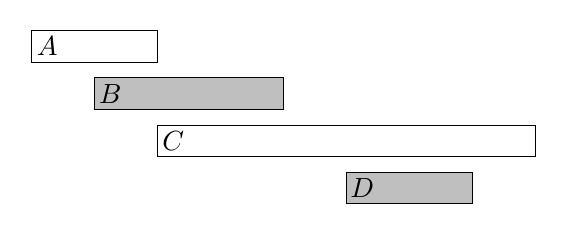
\begin{tikzpicture}[scale=.4]
  \begin{scope}
    \draw (2, 0) rectangle (6, -1);
    \draw[fill=lightgray] (4, -1.5) rectangle (10, -2.5);
    \draw (6, -3) rectangle (18, -4);
    \draw[fill=lightgray] (12, -4.5) rectangle (16, -5.5);
    \node at (2.5,-0.5) {$A$};
    \node at (4.5,-2) {$B$};
    \node at (6.5,-3.5) {$C$};
    \node at (12.5,-5) {$D$};
  \end{scope}
\end{tikzpicture}
\end{center}

\noindent
Tehtävän ratkaisuun on mahdollista 
keksiä useita ahneita algoritmeja,
mutta mikä niistä toimii kaikissa tapauksissa?

\subsubsection*{Algoritmi 1}

Ensimmäinen idea on valita ratkaisuun
mahdollisimman lyhyitä tapahtumia.
Esimerkin tapauksessa tällainen
algoritmi valitsee tapahtumat
\\
\begin{center}
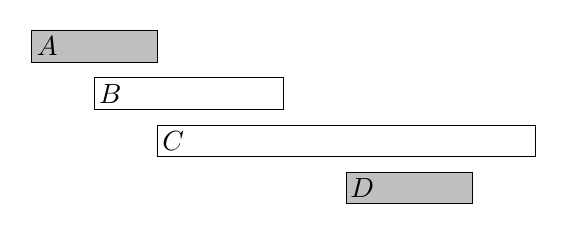
\begin{tikzpicture}[scale=.4]
  \begin{scope}
    \draw[fill=lightgray] (2, 0) rectangle (6, -1);
    \draw (4, -1.5) rectangle (10, -2.5);
    \draw (6, -3) rectangle (18, -4);
    \draw[fill=lightgray] (12, -4.5) rectangle (16, -5.5);
    \node at (2.5,-0.5) {$A$};
    \node at (4.5,-2) {$B$};
    \node at (6.5,-3.5) {$C$};
    \node at (12.5,-5) {$D$};
  \end{scope}
\end{tikzpicture}
\end{center}
ja tuottaa optimiratkaisun.

Lyhimpien tapahtumien valinta ei ole kuitenkaan
aina toimiva strategia.
Algoritmi epäonnistuu esimerkiksi seuraavassa tilanteessa:
\\
\begin{center}
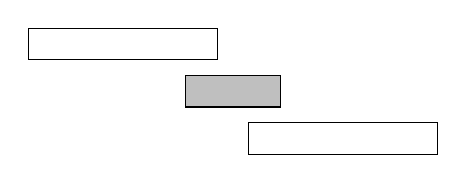
\begin{tikzpicture}[scale=.4]
  \begin{scope}
    \draw (1, 0) rectangle (7, -1);
    \draw[fill=lightgray] (6, -1.5) rectangle (9, -2.5);
    \draw (8, -3) rectangle (14, -4);
  \end{scope}
\end{tikzpicture}
\end{center}

Kun lyhyt tapahtuma valitaan mukaan,
on mahdollista osallistua vain yhteen tapahtumaan.
Kuitenkin valitsemalla pitkät tapahtumat
olisi mahdollista osallistua kahteen tapahtumaan.

\subsubsection*{Algoritmi 2}

Toinen idea on valita aina seuraavaksi tapahtuma,
joka alkaa mahdollisimman aikaisin.
Tämä algoritmi valitsee esimerkissä tapahtumat
\\
\begin{center}
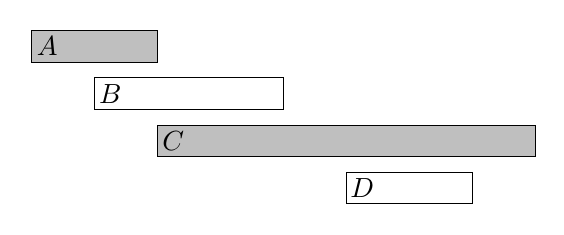
\begin{tikzpicture}[scale=.4]
  \begin{scope}
    \draw[fill=lightgray] (2, 0) rectangle (6, -1);
    \draw (4, -1.5) rectangle (10, -2.5);
    \draw[fill=lightgray] (6, -3) rectangle (18, -4);
    \draw (12, -4.5) rectangle (16, -5.5);
    \node at (2.5,-0.5) {$A$};
    \node at (4.5,-2) {$B$};
    \node at (6.5,-3.5) {$C$};
    \node at (12.5,-5) {$D$};
  \end{scope}
\end{tikzpicture}
\end{center}
ja tuottaa optimiratkaisun.

Tämä algoritmi ei kuitenkaan toimi
esimerkiksi seuraavassa tilanteessa:
\\
\begin{center}
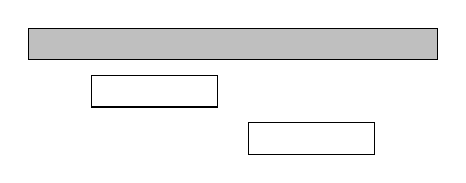
\begin{tikzpicture}[scale=.4]
  \begin{scope}
    \draw[fill=lightgray] (1, 0) rectangle (14, -1);
    \draw (3, -1.5) rectangle (7, -2.5);
    \draw (8, -3) rectangle (12, -4);
  \end{scope}
\end{tikzpicture}
\end{center}

Kun ensimmäisenä alkava tapahtuma
valitaan mukaan, mitään muuta tapahtumaa
ei ole mahdollista valita.
Kuitenkin olisi mahdollista osallistua
kahteen tapahtumaan valitsemalla
kaksi myöhempää tapahtumaa.

\subsubsection*{Algoritmi 3}

Kolmas idea on valita aina seuraavaksi tapahtuma,
joka päättyy mahdollisimman aikaisin.
Tämä algoritmi valitsee esimerkissä tapahtumat
\\
\begin{center}
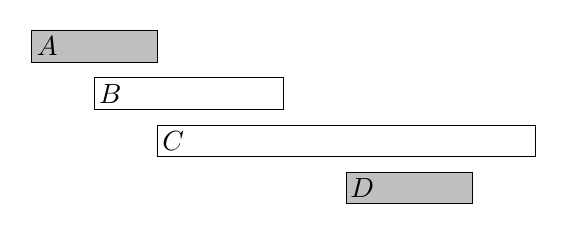
\begin{tikzpicture}[scale=.4]
  \begin{scope}
    \draw[fill=lightgray] (2, 0) rectangle (6, -1);
    \draw (4, -1.5) rectangle (10, -2.5);
    \draw (6, -3) rectangle (18, -4);
    \draw[fill=lightgray] (12, -4.5) rectangle (16, -5.5);
    \node at (2.5,-0.5) {$A$};
    \node at (4.5,-2) {$B$};
    \node at (6.5,-3.5) {$C$};
    \node at (12.5,-5) {$D$};
  \end{scope}
\end{tikzpicture}
\end{center}
ja tuottaa optimiratkaisun.

Osoittautuu, että tämä ahne algoritmi
tuottaa \textit{aina} optimiratkaisun.
Algoritmi toimii, koska on aina kokonaisuuden
kannalta optimaalista valita
ensimmäiseksi tapahtumaksi
mahdollisimman aikaisin päättyvä tapahtuma.
Tämän jälkeen on taas optimaalista
valita seuraava aikatauluun sopiva
mahdollisimman aikaisin
päättyvä tapahtua, jne.

Yksi tapa perustella valintaa on miettiä,
mitä tapahtuu, jos ensimmäiseksi tapahtumaksi
valitaan jokin muu kuin mahdollisimman
aikaisin päättyvä tapahtuma.
Tällainen valinta ei ole koskaan parempi,
koska myöhemmin päättyvän tapahtuman
jälkeen on joko yhtä paljon tai vähemmän
mahdollisuuksia valita seuraavia tapahtumia.

\section{Tehtävät ja deadlinet}

\begin{task}
Annettuna on $n$ tehtävää,
joista jokaisella on kesto ja deadline.
Tehtäväsi on valita järjestys,
jossa suoritat tehtävät.
Saat kustakin tehtävästä $d-x$ pistettä,
missä $d$ on tehtävän deadline ja $x$
on tehtävän valmistumishetki.
Mikä on suurin mahdollinen pistesumma?
\end{task}

Esimerkiksi jos tehtävät ovat

\begin{center}
\begin{tabular}{lll}
tehtävä & kesto & deadline \\
\hline
$A$ & 4 & 2 \\
$B$ & 3 & 5 \\
$C$ & 2 & 7 \\
$D$ & 4 & 5 \\
\end{tabular}
\end{center}

\noindent
niin optimaalinen ratkaisu on suorittaa
tehtävät seuraavasti:

\begin{center}
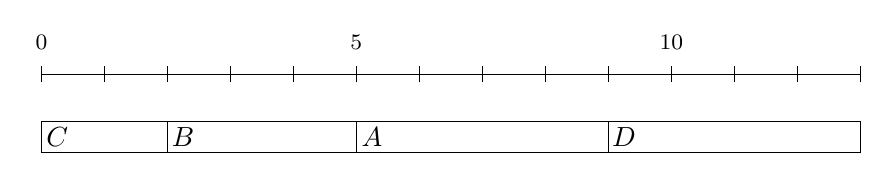
\begin{tikzpicture}[scale=.4]
  \begin{scope}
    \draw (0, 0) rectangle (4, -1);
    \draw (4, 0) rectangle (10, -1);
    \draw (10, 0) rectangle (18, -1);
    \draw (18, 0) rectangle (26, -1);
    \node at (0.5,-0.5) {$C$};
    \node at (4.5,-0.5) {$B$};
    \node at (10.5,-0.5) {$A$};
    \node at (18.5,-0.5) {$D$};

    \draw (0,1.5) -- (26,1.5);
    \foreach \i in {0,2,...,26}
    {
        \draw (\i,1.25) -- (\i,1.75);
    }
    \footnotesize
    \node at (0,2.5) {0};
    \node at (10,2.5) {5};
    \node at (20,2.5) {10};

  \end{scope}
\end{tikzpicture}
\end{center}

Tässä ratkaisussa $C$ tuottaa 5 pistettä,
$B$ tuottaa 0 pistettä, $A$ tuottaa $-7$ pistettä
ja $D$ tuottaa $-8$ pistettä,
joten pistesumma on $-10$.

Yllättävää kyllä, tehtävän optimaalinen ratkaisu
ei riipu lainkaan deadlineista.
Toimiva ahne strategia on
suorittaa tehtävät järjestyksessä keston mukaan
lyhimmästä pisimpään.
Syynä tähän on, että jos missä tahansa vaiheessa
suoritetaan peräkkäin kaksi tehtävää,
joista ensimmäinen kestää toista kauemmin,
tehtävien järjestyksen vaihtaminen parantaa ratkaisua.

Esimerkiksi jos peräkkäin ovat tehtävät

\begin{center}
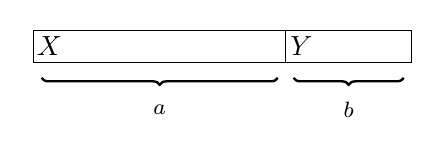
\begin{tikzpicture}[scale=.4]
  \begin{scope}
    \draw (0, 0) rectangle (8, -1);
    \draw (8, 0) rectangle (12, -1);
    \node at (0.5,-0.5) {$X$};
    \node at (8.5,-0.5) {$Y$};

\draw [decoration={brace}, decorate, line width=0.3mm] (7.75,-1.5) -- (0.25,-1.5);
\draw [decoration={brace}, decorate, line width=0.3mm] (11.75,-1.5) -- (8.25,-1.5);

\footnotesize
\node at (4,-2.5) {$a$};
\node at (10,-2.5) {$b$};

  \end{scope}
\end{tikzpicture}
\end{center}

ja $a>b$, niin järjestyksen muuttaminen muotoon

\begin{center}
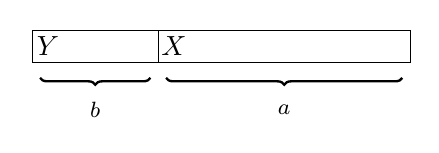
\begin{tikzpicture}[scale=.4]
  \begin{scope}
    \draw (0, 0) rectangle (4, -1);
    \draw (4, 0) rectangle (12, -1);
    \node at (0.5,-0.5) {$Y$};
    \node at (4.5,-0.5) {$X$};

\draw [decoration={brace}, decorate, line width=0.3mm] (3.75,-1.5) -- (0.25,-1.5);
\draw [decoration={brace}, decorate, line width=0.3mm] (11.75,-1.5) -- (4.25,-1.5);

\footnotesize
\node at (2,-2.5) {$b$};
\node at (8,-2.5) {$a$};

  \end{scope}
\end{tikzpicture}
\end{center}

antaa $X$:lle $b$ pistettä vähemmän ja $Y$:lle $a$ pistettä enemmän,
joten kokonaismuutos pistemäärään on $a-b > 0$.
Optimiratkaisussa
kaikille peräkkäin suoritettaville tehtäville
tulee päteä, että lyhyempi tulee ennen pidempää,
mistä seuraa, että tehtävät tulee suorittaa
järjestyksessä keston mukaan.

\section{Keskiluvut}

\subsubsection{Itseisarvosumma}

\begin{task}
Annettuna on $n$ lukua $a_1,a_2,\ldots,a_n$.
Tehtäväsi on etsiä luku $x$, joka minimoi summan
$|a_1-x|+|a_2-x|+\cdots+|a_n-x|.$
\end{task}

Esimerkiksi jos luvut ovat $[1,2,9,2,6]$,
niin paras ratkaisu on $x=2$,
jolloin summaksi tulee
\[
|1-2|+|2-2|+|9-2|+|2-2|+|6-2|=12.
\]

Yleisessä tapauksessa paras valinta $x$:n arvoksi
on lukujen \textit{mediaani}
eli keskimmäinen luku järjestyksessä.
Esimerkiksi luvut $[1,2,9,2,6]$
ovat järjestyksessä $[1,2,2,6,9]$,
joten mediaani on 2.

Mediaanin valinta on paras ratkaisu,
koska jos $x$ on mediaania pienempi,
$x$:n suurentaminen pienentää summaa.
Vastaavasti jos $x$ on mediaania suurempi,
$x$:n pienentäminen pienentää summaa.
Niinpä $x$ kannattaa siirtää mahdollisimman
lähelle mediaania eli optimiratkaisu on
valita $x$ mediaaniksi.

Jos $n$ on parillinen ja mediaaneja on kaksi,
kumpikin mediaani sekä kaikki niiden välillä
olevat luvut tuottavat optimaalisen ratkaisun.

\subsubsection{Neliösumma}

\begin{task}
Annettuna on $n$ lukua $a_1,a_2,\ldots,a_n$.
Tehtäväsi on etsiä luku $x$, joka minimoi summan
$(a_1-x)^2+(a_2-x)^2+\cdots+(a_n-x)^2.$
\end{task}

Esimerkiksi jos luvut ovat $[1,2,9,2,6]$,
niin paras ratkaisu on $x=4$,
jolloin summaksi tulee
\[
(1-4)^2+(2-4)^2+(9-4)^2+(2-4)^2+(6-4)^2=46.
\]

\noindent
Nyt yleisessä tapauksessa
paras valinta $x$:n arvoksi on lukujen
\textit{keskiarvo}.
Esimerkissä lukujen keskiarvo on $(1+2+9+2+6)/5=4$.

Tämän tuloksen voi johtaa järjestämällä summan
uudestaan muotoon

\[
(a_1^2+a_2^2+\cdots+a_n^2)-2x(a_1+a_2+\cdots+a_n)+nx^2.
\]

Ensimmäinen osa ei riipu $x$:stä, joten sen voi jättää huomiotta.
Jäljelle jäävistä osista muodostuu funktio
$nx^2-2xs$, missä $s=a_1+a_2+\cdots+a_n$.
Tämä on ylöspäin aukeava paraabeli,
jonka nollakohdat ovat $x=0$ ja $x=2s/n$
ja pienin arvo on näiden keskikohta
$x=s/n$ eli taulukon lukujen keskiarvo.

\section{Huffmanin koodaus}

\index{Huffmanin koodaus}
\index{koodi}
\index{koodisana}
\index{binäärikoodi}

Tarkastellaan tehtävää, jossa annettuna on merkkijono ja
sille tulee muodostaa \textit{koodi},
jossa jokaista merkkiä vastaa tietty \textit{koodisana}.
Oletetaan, että koodin tulee olla \textit{binäärikoodi}
eli koodisanojen tulee muodostua biteistä 0 ja 1.
Tällaisen koodin avulla voidaan muodostaa merkkijonoa
vastaava bittiesitys.

Yksi mahdollisuus on muodostaa vakiopituinen
koodi eli valita koodisanat niin,
että jokaisen koodisanan pituus on sama.
Esimerkiksi jos aakkostossa on neljä merkkiä,
tarvittava koodisanan pituus on 2:
\begin{center}
\begin{tabular}{rr}
merkki & koodisana \\
\hline
\texttt{A} & 00 \\
\texttt{B} & 01 \\
\texttt{C} & 10 \\
\texttt{D} & 11 \\
\end{tabular}
\end{center}
Nyt esimerkiksi merkkijonoa \texttt{AABACDACA}
vastaa seuraava bittiesitys, jonka pituus on 18 bittiä:
\[000001001011001000\]
Bittiesitystä on kuitenkin mahdollista lyhentää
ottamalla käyttöön koodi, jonka koodisanat voivat
olla keskenään eripituisia.
Ideana on valita usein esiintyville merkeille
lyhyitä koodisanoja ja harvoin esiintyville
merkeille pitkiä koodisanoja.
Tässä tapauksessa hyvä koodi on seuraava:
\begin{center}
\begin{tabular}{rr}
merkki & koodisana \\
\hline
\texttt{A} & 0 \\
\texttt{B} & 110 \\
\texttt{C} & 10 \\
\texttt{D} & 111 \\
\end{tabular}
\end{center}
Nyt merkkijonon \texttt{AABACDACA}
bittiesityksen pituus on vain 15:
\[001100101110100\]
Huomaa, että koodissa ei saa esiintyä kahta koodisanaa,
joista toinen on toisen alkuosa,
koska alkuperäisen merkkijonon palauttaminen
bittiesityksestä ei olisi välttämättä mahdollista.
Esimerkiksi koodissa
\begin{center}
\begin{tabular}{rr}
merkki & koodisana \\
\hline
\texttt{A} & 0 \\
\texttt{B} & 00 \\
\texttt{C} & 1 \\
\texttt{D} & 11 \\
\end{tabular}
\end{center}
koodisan 0 on koodisanan 00 alkuosa.
Tämän seurauksena ei ole mahdollista tietää, tarkoittaako bittiesitys
001 merkkijonoa \texttt{AAC} vai merkkijonoa \texttt{BC}.

\subsubsection{Optimaalinen koodi}

Optimaalinen koodi on sellainen, jossa merkkijonon bittiesitys
on mahdollisimman lyhyt.
Esimerkiksi merkkijonon \texttt{AABACDACA} tapauksessa
optimaalinen koodi on yllä esitetty koodi,
jota käyttäen bittiesityksen pituus on 15.

Huffmanin koodaus on yleinen menetelmä,
jonka avulla voi muodostaa optimaalisen koodin merkkijonolle.
Siinä on ideana muodostaa koodia vastaava binääripuu
merkkien esiintymiskertojen perusteella.

Aluksi jokaista merkkijonon merkkiä vastaa solmu,
jonka painona on merkin esiintymiskertojen määrä merkkijonossa.
Tämän jälkeen joka vaiheessa yhdistetään kaksi solmua,
joiden painot ovat pienimmät.
Näin jatketaan, kunnes koodi on valmis.

Esimerkiksi merkkijonon \texttt{AABACDACA} tapauksessa
alkutilanne on seuraava:

\begin{center}
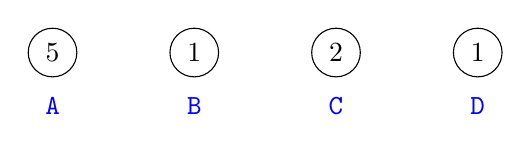
\begin{tikzpicture}[scale=0.9]
\node[draw, circle] (1) at (0,0) {$5$};
\node[draw, circle] (2) at (2,0) {$1$};
\node[draw, circle] (3) at (4,0) {$2$};
\node[draw, circle] (4) at (6,0) {$1$};

\node[color=blue] at (0,-0.75) {\texttt{A}};
\node[color=blue] at (2,-0.75) {\texttt{B}};
\node[color=blue] at (4,-0.75) {\texttt{C}};
\node[color=blue] at (6,-0.75) {\texttt{D}};

%\path[draw,thick,-] (4) -- (5);
\end{tikzpicture}
\end{center}
Merkkiä \texttt{A} vastaavan solmun paino on
5, koska merkki \texttt{A} esiintyy 5 kertaa merkkijonossa.
Muiden solmujen painot on laskettu vastaavalla tavalla.

Ensimmäinen askel on yhdistää merkkejä \texttt{B} ja \texttt{D}
vastaavat solmut, joiden kummankin paino on 1.
Tuloksena on:
\begin{center}
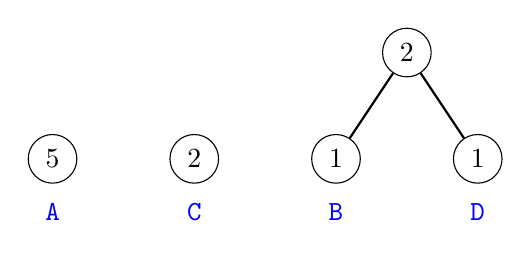
\begin{tikzpicture}[scale=0.9]
\node[draw, circle] (1) at (0,0) {$5$};
\node[draw, circle] (3) at (2,0) {$2$};
\node[draw, circle] (2) at (4,0) {$1$};
\node[draw, circle] (4) at (6,0) {$1$};
\node[draw, circle] (5) at (5,1.5) {$2$};

\node[color=blue] at (0,-0.75) {\texttt{A}};
\node[color=blue] at (2,-0.75) {\texttt{C}};
\node[color=blue] at (4,-0.75) {\texttt{B}};
\node[color=blue] at (6,-0.75) {\texttt{D}};

\path[draw,thick,-] (2) -- (5);
\path[draw,thick,-] (4) -- (5);
\end{tikzpicture}
\end{center}
Tämän jälkeen yhdistetään solmut, joiden paino on 2:
\begin{center}
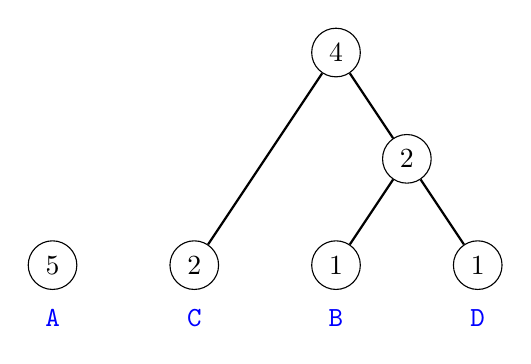
\begin{tikzpicture}[scale=0.9]
\node[draw, circle] (1) at (0,0) {$5$};
\node[draw, circle] (3) at (2,0) {$2$};
\node[draw, circle] (2) at (4,0) {$1$};
\node[draw, circle] (4) at (6,0) {$1$};
\node[draw, circle] (5) at (5,1.5) {$2$};
\node[draw, circle] (6) at (4,3) {$4$};

\node[color=blue] at (0,-0.75) {\texttt{A}};
\node[color=blue] at (2,-0.75) {\texttt{C}};
\node[color=blue] at (4,-0.75) {\texttt{B}};
\node[color=blue] at (6,-0.75) {\texttt{D}};

\path[draw,thick,-] (2) -- (5);
\path[draw,thick,-] (4) -- (5);
\path[draw,thick,-] (3) -- (6);
\path[draw,thick,-] (5) -- (6);
\end{tikzpicture}
\end{center}
Lopuksi yhdistetään kaksi viimeistä solmua:
\begin{center}
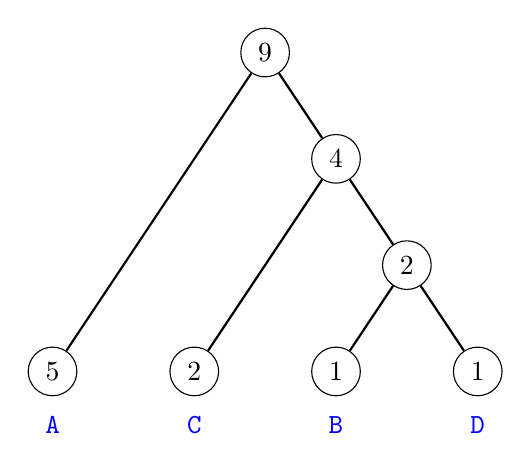
\begin{tikzpicture}[scale=0.9]
\node[draw, circle] (1) at (0,0) {$5$};
\node[draw, circle] (3) at (2,0) {$2$};
\node[draw, circle] (2) at (4,0) {$1$};
\node[draw, circle] (4) at (6,0) {$1$};
\node[draw, circle] (5) at (5,1.5) {$2$};
\node[draw, circle] (6) at (4,3) {$4$};
\node[draw, circle] (7) at (3,4.5) {$9$};

\node[color=blue] at (0,-0.75) {\texttt{A}};
\node[color=blue] at (2,-0.75) {\texttt{C}};
\node[color=blue] at (4,-0.75) {\texttt{B}};
\node[color=blue] at (6,-0.75) {\texttt{D}};

\path[draw,thick,-] (2) -- (5);
\path[draw,thick,-] (4) -- (5);
\path[draw,thick,-] (3) -- (6);
\path[draw,thick,-] (5) -- (6);
\path[draw,thick,-] (1) -- (7);
\path[draw,thick,-] (6) -- (7);
\end{tikzpicture}
\end{center}
Tuloksena olevasta puusta saadaan kutakin merkkiä vastaava
koodisana kulkemalla puun huipulta alas merkkiin asti.
Aina vasemmalle mentäessä koodisanaan tulee bitti 0
ja oikealle mentäessä koodisanaan tulee bitti 1.
Tuloksena on optimaalinen koodi:
\begin{center}
\begin{tabular}{rr}
merkki & koodisana \\
\hline
\texttt{A} & 0 \\
\texttt{B} & 110 \\
\texttt{C} & 10 \\
\texttt{D} & 111 \\
\end{tabular}
\end{center}

\include{luku07}
\chapter{Tasoitettu analyysi}

\index{tasoitettu analyysi@tasoitettu analyysi}

Monen algoritmin aikavaativuuden pystyy laskemaan
suoraan katsomalla algoritmin rakennetta:
mitä silmukoita algoritmissa on ja miten monta
kertaa niitä suoritetaan.
Joskus kuitenkaan näin suoraviivainen analyysi ei
riitä antamaan todellista kuvaa algoritmin tehokkuudesta.

\key{Tasoitettu analyysi} soveltuu sellaisten
algoritmien analyysiin, joiden osana on jokin operaatio,
jonka ajankäyttö vaihtelee.
Ideana on tarkastella yksittäisen operaation
sijasta kaikkia operaatioita algoritmin
aikana ja laskea niiden ajankäytölle yhteinen raja.

\section{Kahden osoittimen tekniikka}

\index{kahden osoittimen tekniikka}

\key{Kahden osoittimen tekniikka} on taulukon käsittelyssä
käytettävä menetelmä, jossa taulukkoa käydään läpi
kahden osoittimen avulla.
Molemmat osoittimet liikkuvat algoritmin aikana,
mutta rajoituksena on, että ne voivat liikkua vain
yhteen suuntaan, mikä takaa, että algoritmi toimii tehokkaasti.

Tutustumme seuraavaksi kahden osoittimen tekniikkaan
kahden esimerkkitehtävän kautta.

\subsubsection{Lukuvälin summa}

\begin{task}
Annettuna on taulukko, jossa on $n$ positiivista kokonaislukua.
Tehtäväsi on tutkia, onko taulukossa väliä,
jossa lukujen summa on $x$.
\end{task}

Ideana on käydä taulukkoa läpi kahden osoittimen
avulla, jotka rajaavat välin taulukosta.
Joka vuorolla vasen osoitin liikkuu
yhden askeleen eteenpäin, kun taas oikea osoitin
liikkuu niin kauan eteenpäin kuin summa on enintään $x$.
Jos välin summaksi tulee tarkalleen $x$, ratkaisu on löytynyt.

Tarkastellaan esimerkkinä algoritmin toimintaa
seuraavassa taulukossa, kun tavoitteena on muodostaa summa $x=8$:
\begin{center}
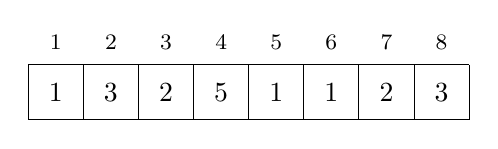
\begin{tikzpicture}[scale=0.7]
\draw (0,0) grid (8,1);

\node at (0.5,0.5) {$1$};
\node at (1.5,0.5) {$3$};
\node at (2.5,0.5) {$2$};
\node at (3.5,0.5) {$5$};
\node at (4.5,0.5) {$1$};
\node at (5.5,0.5) {$1$};
\node at (6.5,0.5) {$2$};
\node at (7.5,0.5) {$3$};

\footnotesize
\node at (0.5,1.4) {$1$};
\node at (1.5,1.4) {$2$};
\node at (2.5,1.4) {$3$};
\node at (3.5,1.4) {$4$};
\node at (4.5,1.4) {$5$};
\node at (5.5,1.4) {$6$};
\node at (6.5,1.4) {$7$};
\node at (7.5,1.4) {$8$};
\end{tikzpicture}
\end{center}

Aluksi osoittimet rajaavat taulukosta välin,
jonka summa on $1+3+2=6$.
Väli ei voi olla tätä suurempi,
koska seuraava luku 5 veisi summan yli $x$:n.

\begin{center}
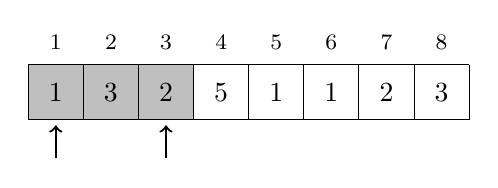
\begin{tikzpicture}[scale=0.7]
\fill[color=lightgray] (0,0) rectangle (3,1);
\draw (0,0) grid (8,1);

\node at (0.5,0.5) {$1$};
\node at (1.5,0.5) {$3$};
\node at (2.5,0.5) {$2$};
\node at (3.5,0.5) {$5$};
\node at (4.5,0.5) {$1$};
\node at (5.5,0.5) {$1$};
\node at (6.5,0.5) {$2$};
\node at (7.5,0.5) {$3$};

\draw[thick,->] (0.5,-0.7) -- (0.5,-0.1);
\draw[thick,->] (2.5,-0.7) -- (2.5,-0.1);

\footnotesize
\node at (0.5,1.4) {$1$};
\node at (1.5,1.4) {$2$};
\node at (2.5,1.4) {$3$};
\node at (3.5,1.4) {$4$};
\node at (4.5,1.4) {$5$};
\node at (5.5,1.4) {$6$};
\node at (6.5,1.4) {$7$};
\node at (7.5,1.4) {$8$};
\end{tikzpicture}
\end{center}

Seuraavaksi vasen osoitin siirtyy askeleen eteenpäin.
Oikea osoitin säilyy paikallaan, koska muuten
summa kasvaisi liian suureksi.

\begin{center}
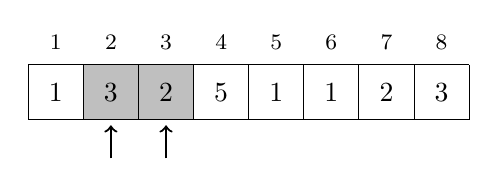
\begin{tikzpicture}[scale=0.7]
\fill[color=lightgray] (1,0) rectangle (3,1);
\draw (0,0) grid (8,1);

\node at (0.5,0.5) {$1$};
\node at (1.5,0.5) {$3$};
\node at (2.5,0.5) {$2$};
\node at (3.5,0.5) {$5$};
\node at (4.5,0.5) {$1$};
\node at (5.5,0.5) {$1$};
\node at (6.5,0.5) {$2$};
\node at (7.5,0.5) {$3$};

\draw[thick,->] (1.5,-0.7) -- (1.5,-0.1);
\draw[thick,->] (2.5,-0.7) -- (2.5,-0.1);

\footnotesize
\node at (0.5,1.4) {$1$};
\node at (1.5,1.4) {$2$};
\node at (2.5,1.4) {$3$};
\node at (3.5,1.4) {$4$};
\node at (4.5,1.4) {$5$};
\node at (5.5,1.4) {$6$};
\node at (6.5,1.4) {$7$};
\node at (7.5,1.4) {$8$};
\end{tikzpicture}
\end{center}

Vasen osoitin siirtyy taas askeleen eteenpäin
ja tällä kertaa oikea osoitin siirtyy kolme askelta
eteenpäin. Muodostuu summa $2+5+1=8$ eli taulukosta
on löytynyt väli, jonka lukujen summa on $x$.

\begin{center}
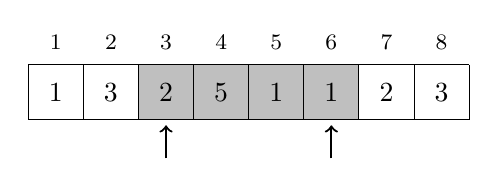
\begin{tikzpicture}[scale=0.7]
\fill[color=lightgray] (2,0) rectangle (6,1);
\draw (0,0) grid (8,1);

\node at (0.5,0.5) {$1$};
\node at (1.5,0.5) {$3$};
\node at (2.5,0.5) {$2$};
\node at (3.5,0.5) {$5$};
\node at (4.5,0.5) {$1$};
\node at (5.5,0.5) {$1$};
\node at (6.5,0.5) {$2$};
\node at (7.5,0.5) {$3$};

\draw[thick,->] (2.5,-0.7) -- (2.5,-0.1);
\draw[thick,->] (5.5,-0.7) -- (5.5,-0.1);

\footnotesize
\node at (0.5,1.4) {$1$};
\node at (1.5,1.4) {$2$};
\node at (2.5,1.4) {$3$};
\node at (3.5,1.4) {$4$};
\node at (4.5,1.4) {$5$};
\node at (5.5,1.4) {$6$};
\node at (6.5,1.4) {$7$};
\node at (7.5,1.4) {$8$};
\end{tikzpicture}
\end{center}

Algoritmin toteutus näyttää seuraavalta:

\begin{lstlisting}
int s = 0, b = 0;
for (int a = 1; a <= n; a++) {
    while (b<n && s+t[b+1] <= x) {
        b++;
        s += t[b];
    }
    if (s == x) {
        // ratkaisu löytyi
    }
    s -= t[a];
}
\end{lstlisting}

Muuttujat $a$ ja $b$ sisältävät vasemman ja oikean
osoittimen kohdan.
Muuttuja $s$ taas laskee lukujen summan välillä.
Joka askeleella $a$ liikkuu askeleen eteenpäin
ja $b$ liikkuu niin kauan kuin summa on enintään $x$.

Algoritmin aikavaativuus riippuu siitä,
kauanko \texttt{while}-silmukan suoritus vie aikaa.
Tämä vaihtelee, koska oikea osoitin voi liikkua
minkä tahansa matkan eteenpäin taulukossa.
Kuitenkin oikea osoitin liikkuu \textit{yhteensä}
$O(n)$ askelta algoritmin aikana, koska se voi
liikkua vain eteenpäin.

Koska sekä vasen että oikea osoitin liikkuvat
$O(n)$ askelta algoritmin aikana,
algoritmin aikavaativuus on $O(n)$.

\subsubsection{Lukujen valinta}

\begin{task}
Annettuna on taulukko, jossa on $n$ kokonaislukua.
Tehtäväsi on tutkia, voiko taulukosta valita kaksi lukua
niin, että niiden summa on $x$.
\end{task}

Tämänkin tehtävän voi ratkaista kahden osoittimen
tekniikalla, kuitenkin niin,
että osoittimet liikkuvat eri suuntiin.
Ideana on järjestää ensin taulukon luvut
pienimmästä suurimpaan ja
sitten käydä taulukkoa läpi kahdella osoittimella,
jotka lähtevät liikkelle sen molemmista päistä.

Vasen osoitin aloittaa taulukon alusta ja
liikkuu joka vaiheessa askeleen eteenpäin.
Oikea osoitin taas aloittaa taulukon lopusta
ja peruuttaa taaksepäin niin kauan, kunnes osoitinten
määrittämän välin lukujen summa on enintään $x$.
Jos summa on tarkalleen $x$, ratkaisu on löytynyt.

Tarkastellaan esimerkkinä algoritmin toimintaa
seuraavassa taulukossa, kun tavoitteena on muodostaa
summa $x=12$:
\begin{center}
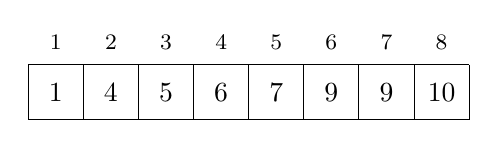
\begin{tikzpicture}[scale=0.7]
\draw (0,0) grid (8,1);

\node at (0.5,0.5) {$1$};
\node at (1.5,0.5) {$4$};
\node at (2.5,0.5) {$5$};
\node at (3.5,0.5) {$6$};
\node at (4.5,0.5) {$7$};
\node at (5.5,0.5) {$9$};
\node at (6.5,0.5) {$9$};
\node at (7.5,0.5) {$10$};

\footnotesize
\node at (0.5,1.4) {$1$};
\node at (1.5,1.4) {$2$};
\node at (2.5,1.4) {$3$};
\node at (3.5,1.4) {$4$};
\node at (4.5,1.4) {$5$};
\node at (5.5,1.4) {$6$};
\node at (6.5,1.4) {$7$};
\node at (7.5,1.4) {$8$};
\end{tikzpicture}
\end{center}

Seuraavassa on algoritmin aloitustilanne.
Lukujen summa on $1+10=11$, joka on pienempi
kuin $x$:n arvo.

\begin{center}
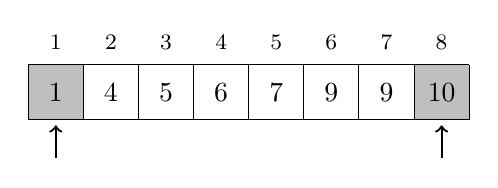
\begin{tikzpicture}[scale=0.7]
\fill[color=lightgray] (0,0) rectangle (1,1);
\fill[color=lightgray] (7,0) rectangle (8,1);
\draw (0,0) grid (8,1);

\node at (0.5,0.5) {$1$};
\node at (1.5,0.5) {$4$};
\node at (2.5,0.5) {$5$};
\node at (3.5,0.5) {$6$};
\node at (4.5,0.5) {$7$};
\node at (5.5,0.5) {$9$};
\node at (6.5,0.5) {$9$};
\node at (7.5,0.5) {$10$};

\draw[thick,->] (0.5,-0.7) -- (0.5,-0.1);
\draw[thick,->] (7.5,-0.7) -- (7.5,-0.1);

\footnotesize
\node at (0.5,1.4) {$1$};
\node at (1.5,1.4) {$2$};
\node at (2.5,1.4) {$3$};
\node at (3.5,1.4) {$4$};
\node at (4.5,1.4) {$5$};
\node at (5.5,1.4) {$6$};
\node at (6.5,1.4) {$7$};
\node at (7.5,1.4) {$8$};
\end{tikzpicture}
\end{center}

Seuraavaksi vasen osoitin liikkuu askeleen eteenpäin.
Oikea osoitin peruuttaa kolme askelta, minkä jälkeen
summana on $4+7=11$.

\begin{center}
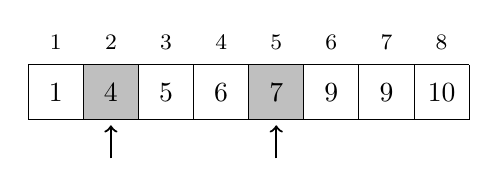
\begin{tikzpicture}[scale=0.7]
\fill[color=lightgray] (1,0) rectangle (2,1);
\fill[color=lightgray] (4,0) rectangle (5,1);
\draw (0,0) grid (8,1);

\node at (0.5,0.5) {$1$};
\node at (1.5,0.5) {$4$};
\node at (2.5,0.5) {$5$};
\node at (3.5,0.5) {$6$};
\node at (4.5,0.5) {$7$};
\node at (5.5,0.5) {$9$};
\node at (6.5,0.5) {$9$};
\node at (7.5,0.5) {$10$};

\draw[thick,->] (1.5,-0.7) -- (1.5,-0.1);
\draw[thick,->] (4.5,-0.7) -- (4.5,-0.1);

\footnotesize
\node at (0.5,1.4) {$1$};
\node at (1.5,1.4) {$2$};
\node at (2.5,1.4) {$3$};
\node at (3.5,1.4) {$4$};
\node at (4.5,1.4) {$5$};
\node at (5.5,1.4) {$6$};
\node at (6.5,1.4) {$7$};
\node at (7.5,1.4) {$8$};
\end{tikzpicture}
\end{center}

Sitten vasen osoitin siirtyy jälleen askeleen eteenpäin.
Oikea osoitin pysyy paikallaan ja ratkaisu $5+7=12$ on löytynyt.

\begin{center}
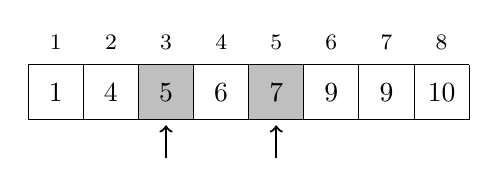
\begin{tikzpicture}[scale=0.7]
\fill[color=lightgray] (2,0) rectangle (3,1);
\fill[color=lightgray] (4,0) rectangle (5,1);
\draw (0,0) grid (8,1);

\node at (0.5,0.5) {$1$};
\node at (1.5,0.5) {$4$};
\node at (2.5,0.5) {$5$};
\node at (3.5,0.5) {$6$};
\node at (4.5,0.5) {$7$};
\node at (5.5,0.5) {$9$};
\node at (6.5,0.5) {$9$};
\node at (7.5,0.5) {$10$};

\draw[thick,->] (2.5,-0.7) -- (2.5,-0.1);
\draw[thick,->] (4.5,-0.7) -- (4.5,-0.1);

\footnotesize
\node at (0.5,1.4) {$1$};
\node at (1.5,1.4) {$2$};
\node at (2.5,1.4) {$3$};
\node at (3.5,1.4) {$4$};
\node at (4.5,1.4) {$5$};
\node at (5.5,1.4) {$6$};
\node at (6.5,1.4) {$7$};
\node at (7.5,1.4) {$8$};
\end{tikzpicture}
\end{center}

Algoritmin alussa taulukon järjestäminen vie
aikaa $O(n \log n)$.
Tämän jälkeen vasen osoitin liikkuu $O(n)$ askelta
eteenpäin ja oikea osoitin liikkuu $O(n)$ askelta
taaksepäin, mihin kuluu aikaa $O(n)$.
Algoritmin kokonaisaikavaativuus on siis $O(n \log n)$.

Huomaa, että tehtävän voi ratkaista myös 
toisella tavalla ajassa
$O(n \log n)$ binäärihaun avulla.
Tässä ratkaisussa jokaiselle taulukon luvulle
etsitään binäärihaulla toista lukua niin,
että lukujen summa olisi yhteensä $x$.
Binäärihaku suoritetaan $n$ kertaa ja
jokainen binäärihaku vie aikaa $O(\log n)$.

\section{Lähin pienempi edeltäjä}

\index{lzhin pienempi edeltxjx@lähin pienempi edeltäjä}

Tasoitetun analyysin avulla arvioidaan usein
tietorakenteeseen tehtävien operaatioiden määrää.
Algoritmin operaatiot voivat jakautua epätasaisesti
niin, että useimmat operaatiot tehdään tietyssä
algoritmin vaiheessa. Näin on seuraavassa tehtävässä:

\begin{task}
Annettuna on taulukko, jossa on $n$ lukua.
Tehtäväsi on etsiä jokaiselle luvulle
sitä lähinnä oleva pienempi luku
taulukon alkuosassa
tai todeta, että tällaista lukua ei ole olemassa.
\end{task}

Tehokas ratkaisu tehtävään on käydä
taulukko läpi alusta loppuun ja pitää samalla yllä ketjua,
jonka ensimmäinen luku on käsiteltävä taulukon luku
ja jokainen seuraava luku on luvun lähin
pienempi edeltäjä.
Jos ketjussa on vain yksi luku,
käsiteltävällä luvulla ei ole pienempää edeltäjää.

Joka askeleella ketjun alusta poistetaan lukuja
niin kauan, kunnes ketjun ensimmäinen luku on 
pienempi kuin käsiteltävä taulukon luku tai ketju on tyhjä.
Tämän jälkeen käsiteltävä luku lisätään ketjun alkuun.

Tarkastellaan esimerkkinä algoritmin toimintaa
seuraavassa taulukossa:

\begin{center}
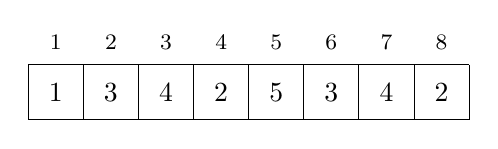
\begin{tikzpicture}[scale=0.7]
\draw (0,0) grid (8,1);

\node at (0.5,0.5) {$1$};
\node at (1.5,0.5) {$3$};
\node at (2.5,0.5) {$4$};
\node at (3.5,0.5) {$2$};
\node at (4.5,0.5) {$5$};
\node at (5.5,0.5) {$3$};
\node at (6.5,0.5) {$4$};
\node at (7.5,0.5) {$2$};

\footnotesize
\node at (0.5,1.4) {$1$};
\node at (1.5,1.4) {$2$};
\node at (2.5,1.4) {$3$};
\node at (3.5,1.4) {$4$};
\node at (4.5,1.4) {$5$};
\node at (5.5,1.4) {$6$};
\node at (6.5,1.4) {$7$};
\node at (7.5,1.4) {$8$};
\end{tikzpicture}
\end{center}

Aluksi luvut 1, 3 ja 4 liittyvät ketjuun, koska jokainen luku on
edellistä suurempi. Siis luvun 4 lähin pienempi edeltäjä on luku 3,
jonka lähin pienempi edeltäjä on puolestaan luku 1. Tilanne näyttää tältä:

\begin{center}
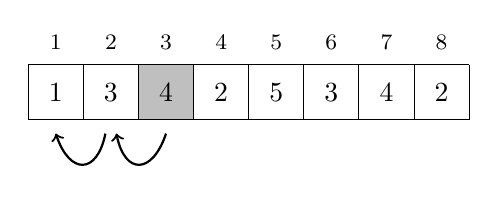
\begin{tikzpicture}[scale=0.7]
\fill[color=lightgray] (2,0) rectangle (3,1);
\draw (0,0) grid (8,1);

\node at (0.5,0.5) {$1$};
\node at (1.5,0.5) {$3$};
\node at (2.5,0.5) {$4$};
\node at (3.5,0.5) {$2$};
\node at (4.5,0.5) {$5$};
\node at (5.5,0.5) {$3$};
\node at (6.5,0.5) {$4$};
\node at (7.5,0.5) {$2$};

\draw[thick,->] (2.5,-0.25) .. controls (2.25,-1.00) and (1.75,-1.00) .. (1.6,-0.25);
\draw[thick,->] (1.4,-0.25) .. controls (1.25,-1.00) and (0.75,-1.00) .. (0.5,-0.25);

\footnotesize
\node at (0.5,1.4) {$1$};
\node at (1.5,1.4) {$2$};
\node at (2.5,1.4) {$3$};
\node at (3.5,1.4) {$4$};
\node at (4.5,1.4) {$5$};
\node at (5.5,1.4) {$6$};
\node at (6.5,1.4) {$7$};
\node at (7.5,1.4) {$8$};
\end{tikzpicture}
\end{center}

Taulukon seuraava luku 2 on pienempi kuin ketjun kaksi ensimmäistä lukua 4 ja 3.
Niinpä luvut 4 ja 3 poistetaan ketjusta, minkä jälkeen luku 2
lisätään ketjun alkuun. Sen lähin pienempi edeltäjä on luku 1:

\begin{center}
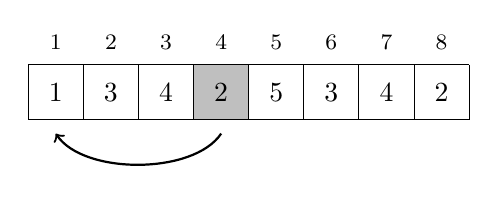
\begin{tikzpicture}[scale=0.7]
\fill[color=lightgray] (3,0) rectangle (4,1);
\draw (0,0) grid (8,1);

\node at (0.5,0.5) {$1$};
\node at (1.5,0.5) {$3$};
\node at (2.5,0.5) {$4$};
\node at (3.5,0.5) {$2$};
\node at (4.5,0.5) {$5$};
\node at (5.5,0.5) {$3$};
\node at (6.5,0.5) {$4$};
\node at (7.5,0.5) {$2$};

\draw[thick,->] (3.5,-0.25) .. controls (3.00,-1.00) and (1.00,-1.00) .. (0.5,-0.25);

\footnotesize
\node at (0.5,1.4) {$1$};
\node at (1.5,1.4) {$2$};
\node at (2.5,1.4) {$3$};
\node at (3.5,1.4) {$4$};
\node at (4.5,1.4) {$5$};
\node at (5.5,1.4) {$6$};
\node at (6.5,1.4) {$7$};
\node at (7.5,1.4) {$8$};
\end{tikzpicture}
\end{center}

Seuraava luku 5 on suurempi kuin luku 2,
joten se lisätään suoraan ketjun alkuun ja
sen lähin pienempi edeltäjä on luku 2:

\begin{center}
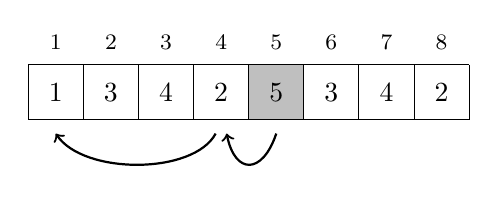
\begin{tikzpicture}[scale=0.7]
\fill[color=lightgray] (4,0) rectangle (5,1);
\draw (0,0) grid (8,1);

\node at (0.5,0.5) {$1$};
\node at (1.5,0.5) {$3$};
\node at (2.5,0.5) {$4$};
\node at (3.5,0.5) {$2$};
\node at (4.5,0.5) {$5$};
\node at (5.5,0.5) {$3$};
\node at (6.5,0.5) {$4$};
\node at (7.5,0.5) {$2$};

\draw[thick,->] (3.4,-0.25) .. controls (3.00,-1.00) and (1.00,-1.00) .. (0.5,-0.25);
\draw[thick,->] (4.5,-0.25) .. controls (4.25,-1.00) and (3.75,-1.00) .. (3.6,-0.25);

\footnotesize
\node at (0.5,1.4) {$1$};
\node at (1.5,1.4) {$2$};
\node at (2.5,1.4) {$3$};
\node at (3.5,1.4) {$4$};
\node at (4.5,1.4) {$5$};
\node at (5.5,1.4) {$6$};
\node at (6.5,1.4) {$7$};
\node at (7.5,1.4) {$8$};
\end{tikzpicture}
\end{center}

Algoritmi jatkaa samalla tavalla taulukon loppuun
ja selvittää jokaisen luvun lähimmän
pienemmän edeltäjän.
Mutta kuinka tehokas algoritmi on?

Algoritmin tehokkuus riippuu siitä,
kauanko ketjun käsittelyyn kuluu aikaa yhteensä.
Jos uusi luku on suurempi kuin ketjun ensimmäinen
luku, se vain lisätään ketjun alkuun,
mikä on tehokasta.
Joskus taas ketjussa voi olla useita
suurempia lukuja, joiden poistaminen vie aikaa.

Oleellista on kuitenkin, että jokainen
taulukossa oleva luku liittyy
tarkalleen kerran ketjuun ja poistuu
korkeintaan kerran ketjusta.
Niinpä jokainen luku aiheuttaa $O(1)$
ketjuun liittyvää operaatiota, ja tämän
seurauksena algoritmin kokonaisaikavaativuus on $O(n)$.

\section{Liukuvan ikkunan minimi}

\index{liukuvan ikkunan minimi@liukuvan ikkunan minimi}

\begin{task}
Annettuna on taulukko, jossa on $n$ lukua,
sekä kokonaisluku $k$.
Taulukon halki kulkee ikkuna, joka käy
läpi taulukon kaikki $k$-kokoiset välit.
Tehtäväsi on ilmoittaa jokaisesta ikkunasta
pienin välillä oleva luku.
\end{task}

Tämän tehtävän voi ratkaista lähes samalla
tavalla kuin edellisen tehtävän.
Ideana on pitää yllä ketjua, jonka alussa
on ikkunan viimeinen luku ja jossa jokainen
luku on edellistä pienempi. Joka vaiheessa
ketjun viimeinen luku on ikkunan pienin luku.

Kun liukuva ikkuna liikkuu eteenpäin ja välille
tulee uusi luku, ketjusta poistetaan kaikki luvut,
jotka ovat uutta lukua suurempia.
Tämän jälkeen uusi luku lisätään ketjun alkuun.
Lisäksi jos ketjun viimeinen luku ei enää kuulu
välille, se poistetaan ketjusta.

Tarkastellaan esimerkkinä, kuinka algoritmi selvittää
minimit seuraavassa taulukossa,
kun ikkunan koko $k=4$.

\begin{center}
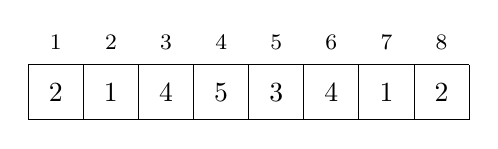
\begin{tikzpicture}[scale=0.7]
\draw (0,0) grid (8,1);

\node at (0.5,0.5) {$2$};
\node at (1.5,0.5) {$1$};
\node at (2.5,0.5) {$4$};
\node at (3.5,0.5) {$5$};
\node at (4.5,0.5) {$3$};
\node at (5.5,0.5) {$4$};
\node at (6.5,0.5) {$1$};
\node at (7.5,0.5) {$2$};

\footnotesize
\node at (0.5,1.4) {$1$};
\node at (1.5,1.4) {$2$};
\node at (2.5,1.4) {$3$};
\node at (3.5,1.4) {$4$};
\node at (4.5,1.4) {$5$};
\node at (5.5,1.4) {$6$};
\node at (6.5,1.4) {$7$};
\node at (7.5,1.4) {$8$};
\end{tikzpicture}
\end{center}

Liukuva ikkuna aloittaa matkansa taulukon vasemmasta reunasta.
Ensimmäisessä ikkunan sijainnissa pienin luku on 1:

\begin{center}
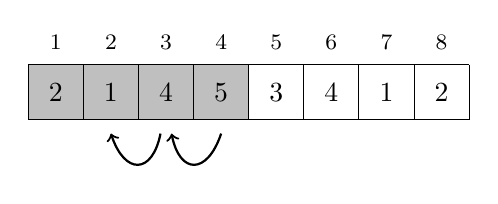
\begin{tikzpicture}[scale=0.7]
\fill[color=lightgray] (0,0) rectangle (4,1);
\draw (0,0) grid (8,1);

\node at (0.5,0.5) {$2$};
\node at (1.5,0.5) {$1$};
\node at (2.5,0.5) {$4$};
\node at (3.5,0.5) {$5$};
\node at (4.5,0.5) {$3$};
\node at (5.5,0.5) {$4$};
\node at (6.5,0.5) {$1$};
\node at (7.5,0.5) {$2$};

\footnotesize
\node at (0.5,1.4) {$1$};
\node at (1.5,1.4) {$2$};
\node at (2.5,1.4) {$3$};
\node at (3.5,1.4) {$4$};
\node at (4.5,1.4) {$5$};
\node at (5.5,1.4) {$6$};
\node at (6.5,1.4) {$7$};
\node at (7.5,1.4) {$8$};

\draw[thick,->] (3.5,-0.25) .. controls (3.25,-1.00) and (2.75,-1.00) .. (2.6,-0.25);
\draw[thick,->] (2.4,-0.25) .. controls (2.25,-1.00) and (1.75,-1.00) .. (1.5,-0.25);

\end{tikzpicture}
\end{center}

Kun ikkuna siirtyy eteenpäin, mukaan tulee luku 3,
joka on pienempi kuin luvut 5 ja 4 ketjun alussa.
Niinpä luvut 5 ja 4 poistuvat ketjusta ja luku 3
siirtyy sen alkuun. Pienin luku on edelleen 1.

\begin{center}
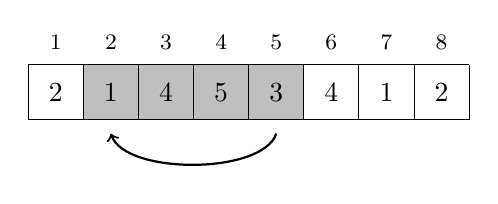
\begin{tikzpicture}[scale=0.7]
\fill[color=lightgray] (1,0) rectangle (5,1);
\draw (0,0) grid (8,1);

\node at (0.5,0.5) {$2$};
\node at (1.5,0.5) {$1$};
\node at (2.5,0.5) {$4$};
\node at (3.5,0.5) {$5$};
\node at (4.5,0.5) {$3$};
\node at (5.5,0.5) {$4$};
\node at (6.5,0.5) {$1$};
\node at (7.5,0.5) {$2$};

\footnotesize
\node at (0.5,1.4) {$1$};
\node at (1.5,1.4) {$2$};
\node at (2.5,1.4) {$3$};
\node at (3.5,1.4) {$4$};
\node at (4.5,1.4) {$5$};
\node at (5.5,1.4) {$6$};
\node at (6.5,1.4) {$7$};
\node at (7.5,1.4) {$8$};

\draw[thick,->] (4.5,-0.25) .. controls (4.25,-1.00) and (1.75,-1.00) .. (1.5,-0.25);

\end{tikzpicture}
\end{center}

Ikkuna siirtyy taas eteenpäin, jonka seurauksena pienin luku 1
putoaa pois ikkunasta. Niinpä se poistetaan ketjun lopusta
ja uusi pienin luku on 3. Lisäksi uusi ikkunaan tuleva luku 4
lisätään ketjun alkuun.

\begin{center}
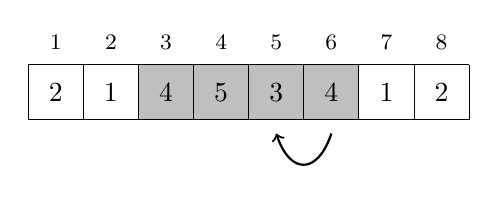
\begin{tikzpicture}[scale=0.7]
\fill[color=lightgray] (2,0) rectangle (6,1);
\draw (0,0) grid (8,1);

\node at (0.5,0.5) {$2$};
\node at (1.5,0.5) {$1$};
\node at (2.5,0.5) {$4$};
\node at (3.5,0.5) {$5$};
\node at (4.5,0.5) {$3$};
\node at (5.5,0.5) {$4$};
\node at (6.5,0.5) {$1$};
\node at (7.5,0.5) {$2$};

\footnotesize
\node at (0.5,1.4) {$1$};
\node at (1.5,1.4) {$2$};
\node at (2.5,1.4) {$3$};
\node at (3.5,1.4) {$4$};
\node at (4.5,1.4) {$5$};
\node at (5.5,1.4) {$6$};
\node at (6.5,1.4) {$7$};
\node at (7.5,1.4) {$8$};

\draw[thick,->] (5.5,-0.25) .. controls (5.25,-1.00) and (4.75,-1.00) .. (4.5,-0.25);
\end{tikzpicture}
\end{center}

Seuraavaksi ikkunaan tuleva luku 1 on pienempi
kuin kaikki ketjussa olevat luvut.
Tämän seurauksena koko ketju tyhjentyy ja
siihen jää vain luku 1:

\begin{center}
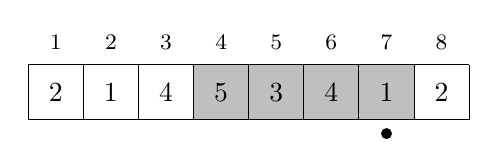
\begin{tikzpicture}[scale=0.7]
\fill[color=lightgray] (3,0) rectangle (7,1);
\draw (0,0) grid (8,1);

\node at (0.5,0.5) {$2$};
\node at (1.5,0.5) {$1$};
\node at (2.5,0.5) {$4$};
\node at (3.5,0.5) {$5$};
\node at (4.5,0.5) {$3$};
\node at (5.5,0.5) {$4$};
\node at (6.5,0.5) {$1$};
\node at (7.5,0.5) {$2$};

\footnotesize
\node at (0.5,1.4) {$1$};
\node at (1.5,1.4) {$2$};
\node at (2.5,1.4) {$3$};
\node at (3.5,1.4) {$4$};
\node at (4.5,1.4) {$5$};
\node at (5.5,1.4) {$6$};
\node at (6.5,1.4) {$7$};
\node at (7.5,1.4) {$8$};

\fill[color=black] (6.5,-0.25) circle (0.1);

%\draw[thick,->] (5.5,-0.25) .. controls (5.25,-1.00) and (4.75,-1.00) .. (4.5,-0.25);
\end{tikzpicture}
\end{center}

Lopuksi ikkuna saapuu viimeiseen sijaintiinsa.
Luku 2 lisätään ketjun alkuun,
mutta ikkunan pienin luku on edelleen 1.

\begin{center}
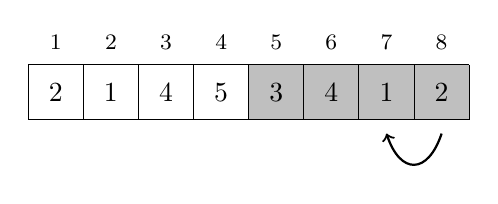
\begin{tikzpicture}[scale=0.7]
\fill[color=lightgray] (4,0) rectangle (8,1);
\draw (0,0) grid (8,1);

\node at (0.5,0.5) {$2$};
\node at (1.5,0.5) {$1$};
\node at (2.5,0.5) {$4$};
\node at (3.5,0.5) {$5$};
\node at (4.5,0.5) {$3$};
\node at (5.5,0.5) {$4$};
\node at (6.5,0.5) {$1$};
\node at (7.5,0.5) {$2$};

\footnotesize
\node at (0.5,1.4) {$1$};
\node at (1.5,1.4) {$2$};
\node at (2.5,1.4) {$3$};
\node at (3.5,1.4) {$4$};
\node at (4.5,1.4) {$5$};
\node at (5.5,1.4) {$6$};
\node at (6.5,1.4) {$7$};
\node at (7.5,1.4) {$8$};

\draw[thick,->] (7.5,-0.25) .. controls (7.25,-1.00) and (6.75,-1.00) .. (6.5,-0.25);
\end{tikzpicture}
\end{center}

Tässäkin algoritmissa jokainen taulukon luku lisätään
ketjuun tarkalleen kerran ja poistetaan ketjusta korkeintaan kerran,
joko ketjun alusta tai ketjun lopusta.
Niinpä algoritmin kokonaisaikavaativuus on $O(n)$.




\include{luku09}
\chapter{Bittien käsittely}

Tietokone käsittelee tietoa sisäisesti bitteinä
eli numeroina 0 ja 1.
Tässä luvussa tutustumme tarkemmin kokonaisluvun
bittiesitykseen sekä bittioperaatioihin,
jotka muokkaavat luvun bittejä.
Osoittautuu, että näistä operaatioista on
monenlaista hyötyä algoritmien ohjelmoinnissa.

\section{Luvun bittiesitys}

\index{bittiesitys}

Luvun bittiesitys ilmaisee, mistä 2:n potensseista
luku muodostuu. Esimerkiksi luvun 43 bittiesitys on 101011, koska
$43 = 2^5 + 2^3 + 2^1 + 2^0$
eli oikealta lukien bitit 0, 1, 3 ja 5 ovat ykkösiä
ja kaikki muut bitit ovat nollia.

Tietokoneessa luvun bittiesityksen
bittien määrä on kiinteä ja riippuu käytetystä tietotyypistä.
Esimerkiksi C++:n \texttt{int}-tyyppi on tavallisesti 32-bittinen,
jolloin \texttt{int}-luku tallennetaan 32 bittinä.
Tällöin esimerkiksi luvun 43 bittiesitys \texttt{int}-lukuna on seuraava:

\[00000000000000000000000000101011\]

Luvun bittiesitys on joko etumerkillinen (\textit{signed})
tai etumerkitön (\textit{unsigned}).
Etumerkillisen bittiesityksen ensimmäinen bitti on etumerkki
($+$ tai $-$) ja $n$ bitillä voi esittää luvut $-2^{n-1} \ldots 2^{n-1}-1$.
Jos taas bittiesitys on etumerkitön,
kaikki bitit kuuluvat lukuun ja $n$ bitillä voi esittää luvut $0 \ldots 2^n-1$.

Etumerkillisessä bittiesityksessä ei-negatiivisen luvun
ensimmäinen bitti on 0 ja negatiivisen luvun
ensimmäinen bitti on 1.
Bittiesityksenä on kahden komplementti
(\textit{two's complement}),
jossa positiivisesta luvusta saa negatiivisen muuttamalla
kaikki bitit käänteiseksi ja lisäämällä
tulokseen yksi.

Esimerkiksi luvun $-43$ esitys \texttt{int}-lukuna on seuraava:

\[11111111111111111111111111010101\]

Etumerkillisen ja etumerkittömän bittiesityksen
yhteys on, että etumerkillisen luvun $-x$
ja etumerkittömän luvun $2^n-x$ bittiesitykset ovat samat.
Niinpä yllä oleva bittiesitys tarkoittaa
etumerkittömänä lukua $2^{32}-43$.

C++:ssa luvut ovat oletuksena etumerkillisiä,
mutta avainsanan \texttt{unsigned} avulla
luvusta saa etumerkittömän.
Esimerkiksi koodissa

\begin{lstlisting}
int x = -43;
unsigned int y = x;
cout << x << "\n"; // -43
cout << y << "\n"; // 4294967253
\end{lstlisting}

etumerkillistä lukua $x=-43$ vastaa etumerkitön luku $y=2^{32}-43$.

Jos luvun suuruus menee käytössä
olevan bittiesityksen ulkopuolelle,
niin luku pyörähtää ympäri.
Etumerkillisessä bittiesityksessä
luvusta $2^{n-1}-1$ seuraava luku on $-2^{n-1}$
ja vastaavasti etumerkittömässä bittiesityksessä
luvusta $2^n-1$ seuraava luku on $0$.
Esimerkiksi koodissa

\begin{lstlisting}
int x = 2147483647
cout << x << "\n"; // 2147483647
x++;
cout << x << "\n"; // -2147483648
\end{lstlisting}

muuttuja $x$ pyörähtää ympäri luvusta $2^{31}-1$ lukuun $-2^{31}$.

\section{Bittioperaatiot}

\newcommand\XOR{\mathbin{\char`\^}}

\subsubsection{And-operaatio}

And-operaatio $x$ \& $y$ tuottaa luvun,
jossa on ykkösbitti niissä kohdissa,
joissa molemmissa luvuissa $x$ ja $y$ on ykkösbitti.
Esimerkiksi $22$ \& $26$ = 18, koska

\begin{center}
\begin{tabular}{rrr}
& 10110 & (22)\\
\& & 11010 & (26) \\
\hline
 = & 10010 & (18) \\
\end{tabular}
\end{center}

And-operaation avulla voi tarkastaa luvun parillisuuden,
koska $x$ \& $1$ = 0, jos luku on parillinen,
ja $x$ \& $1$ = 1, jos luku on pariton.

\subsubsection{Or-operaatio}

Or-operaatio $x$ | $y$ tuottaa luvun,
jossa on ykkösbitti niissä kohdissa,
joissa ainakin toisessa luvuista $x$ ja $y$ on ykkösbitti.
Esimerkiksi $22$ | $26$ = 30, koska

\begin{center}
\begin{tabular}{rrr}
& 10110 & (22)\\
| & 11010 & (26) \\
\hline
 = & 11110 & (30) \\
\end{tabular}
\end{center}

\subsubsection{Xor-operaatio}

Xor-operaatio $x$ $\XOR$ $y$ tuottaa luvun,
jossa on ykkösbitti niissä kohdissa,
joissa tarkalleen toisessa luvuista $x$ ja $y$ on ykkösbitti.
Esimerkiksi $22$ $\XOR$ $26$ = 12, koska

\begin{center}
\begin{tabular}{rrr}
& 10110 & (22)\\
$\XOR$ & 11010 & (26) \\
\hline
 = & 01100 & (12) \\
\end{tabular}
\end{center}

\subsubsection{Not-operaatio}

Not-operaatio \textasciitilde$x$ tuottaa luvun,
jossa kaikki $x$:n bitit on muutettu käänteisiksi.
Operaatiolle pätee kaava \textasciitilde$x = -x-1$,
esimerkiksi \textasciitilde$29 = -30$.

Not-operaation toiminta bittitasolla riippuu siitä,
montako bittiä luvun bittiesityksessä on,
koska operaatio vaikuttaa kaikkiin luvun bitteihin.
Esimerkiksi 32-bittisenä \texttt{int}-lukuna
tilanne on seuraava:

\begin{center}
\begin{tabular}{rrrr}
$x$ & = & 29 &   00000000000000000000000000011101 \\
\textasciitilde$x$ & = & 30 & 11111111111111111111111111100010 \\
\end{tabular}
\end{center}


\subsubsection{Bittisiirrot}

Vasen bittisiirto $x < < k$ tuottaa luvun, jossa luvun $x$ bittejä
on siirretty $k$ askelta vasemmalle
(luvun loppuun tulee $k$ nollabittiä).
Oikea bittisiirto $x > > k$ tuottaa puolestaan
luvun, jossa luvun $x$ bittejä
on siirretty $k$ askelta oikealle 
(luvun lopusta lähtee pois $k$ viimeistä bittiä).

Esimerkiksi $14 < < 2 = 56$,
koska $14$ on bitteinä 1110,
josta tulee bittisiirron jälkeen 111000 eli $56$.
Vastaavasti $49 > > 3 = 6$,
koska $49$ on bitteinä 110001,
josta tulee bittisiirron jälkeen 110 eli $6$.

Huomaa, että vasen bittisiirto $x < < k$
vastaa luvun $x$ kertomista $2^k$:lla
ja oikea bittisiirto $x > > k$
vastaa luvun $x$ jakamista $2^k$:lla
alaspäin pyöristäen.

\subsubsection{Bittien käsittely}

Luvun bitit indeksoidaan oikealta vasemmalle
nollasta alkaen.
Luvussa $1 < < k$ on tarkalleen yksi ykkösbitti
kohdassa $k$, joten sen avulla voi käsitellä
muiden lukujen yksittäisiä bittejä.

Luvun $x$ bitti $k$ on ykkösbitti, jos
$x$ \& $(1 < < k) = (1 < < k)$.
Lauseke $x$ | $(1 < < k)$ asettaa luvun $x$ bitin $k$
ykköseksi, lauseke
$x$ \& \textasciitilde $(1 < < k)$
asettaa luvun $x$ bitin $k$ nollaksi ja
lauseke $x$ $\XOR$ $(1 < < k)$
muuttaa luvun $x$ bitin $k$ käänteiseksi.
% 
% Seuraava koodi muuttaa luvun bittejä:
% 
% \begin{lstlisting}
% int x = 181; // 10110101
% cout << (x|(1<<2)) << "\n"; // 181 = 10110101
% cout << (x|(1<<3)) << "\n"; // 189 = 10111101
% cout << (x&~(1<<2)) << "\n"; // 177 = 10110001
% cout << (x&~(1<<3)) << "\n"; // 181 = 10110101
% cout << (x^(1<<2)) << "\n"; // 177 = 10110001
% cout << (x^(1<<3)) << "\n"; // 189 = 10111101
% \end{lstlisting}
% 
% % Bittiesityksen vasemmanpuoleisin bitti on eniten merkitsevä
% % (\textit{most significant}) ja
% % oikeanpuoleisin bitti on vähiten merkitsevä (\textit{least significant}).

Lauseke $x$ \& $(x-1)$ muuttaa luvun $x$ viimeisen
ykkösbitin nollaksi, ja lauseke $x$ \& $-x$ nollaa
luvun $x$ kaikki bitit paitsi viimeisen ykkösbitin.
Lauseke $x$ | $(x-1)$ vuorostaan muuttaa kaikki
viimeisen ykkösbitin jälkeiset bitit ykkösiksi.

Huomaa myös, että positiivinen luku $x$ on muotoa $2^k$,
jos $x$ \& $(x-1) = 0$.
% 
% Seuraava koodi esittelee operaatioita:
% 
% \begin{lstlisting}
% int x = 168; // 10101000
% cout << (x&(x-1)) << "\n"; // 160 = 10100000
% cout << (x&-x) << "\n"; // 8 = 00001000
% cout << (x|(x-1)) << "\n"; // 175 = 10101111
% \end{lstlisting}

\subsubsection*{Lisäfunktiot}

GCC:n g++-kääntäjä sisältää mm. seuraavat funktiot
bittien käsittelyyn:

\begin{itemize}
\item
$\texttt{\_\_builtin\_clz}(x)$:
nollien määrä bittiesityksen alussa
\item
$\texttt{\_\_builtin\_ctz}(x)$:
nollien määrä bittiesityksen lopussa
\item
$\texttt{\_\_builtin\_popcount}(x)$:
ykkösten määrä bittiesityksessä
\item
$\texttt{\_\_builtin\_parity}(x)$:
ykkösten määrän parillisuus
\end{itemize}

\begin{samepage}
\noindent
Nämä funktiot käsittelevät \texttt{int}-lukuja,
mutta funktioista on myös \texttt{long long} -versiot,
joiden lopussa on pääte \texttt{ll}.

Seuraava koodi esittelee funktioiden käyttöä:

\begin{lstlisting}
int x = 5328; // 00000000000000000001010011010000
cout << __builtin_clz(x) << "\n"; // 19
cout << __builtin_ctz(x) << "\n"; // 4
cout << __builtin_popcount(x) << "\n"; // 5
cout << __builtin_parity(x) << "\n"; // 1
\end{lstlisting}
\end{samepage}

\section{Joukon bittiesitys}

Joukon $\{0,1,2,\ldots,n-1\}$
jokaista osajoukkoa
vastaa $n$-bittinen luku,
jossa ykkösbitit ilmaisevat,
mitkä alkiot ovat mukana osajoukossa.
Esimerkiksi joukkoa $\{1,3,4,8\}$
vastaa bittiesitys 100011010 eli luku
$2^8+2^4+2^3+2^1=282$.

Joukon bittiesitys vie vähän muistia,
koska tieto kunkin alkion kuulumisesta
osajoukkoon vie vain yhden bitin tilaa.
Lisäksi bittimuodossa tallennettua joukkoa
on tehokasta käsitellä bittioperaatioilla.

\subsubsection{Joukon käsittely}

Seuraavan koodin muuttuja $x$
sisältää joukon $\{0,1,2,\ldots,31\}$
osajoukon.
Koodi lisää luvut 1, 3, 4 ja 8
joukkoon ja tulostaa
joukon sisällön.

\begin{lstlisting}
// x on tyhjä joukko
int x = 0;
// lisätään luvut 1, 3, 4 ja 8 joukkoon
x |= (1<<1);
x |= (1<<3);
x |= (1<<4);
x |= (1<<8);
// tulostetaan joukon sisältö
for (int i = 0; i < 32; i++) {
    if (x&(1<<i)) cout << i << " ";
}
cout << "\n";
\end{lstlisting}
Koodin tulostus on seuraava:
\begin{lstlisting}
1 3 4 8
\end{lstlisting}

\noindent
Nyt joukko-operaatiot voi toteuttaa bittioperaatioilla:
\begin{itemize}
\item $a$ \& $b$ on joukkojen $a$ ja $b$ leikkaus $a \cap b$
(tämä sisältää alkiot,
jotka ovat kummassakin joukossa)
\item $a$ | $b$ on joukkojen $a$ ja $b$ yhdiste $a \cup b$
(tämä sisältää alkiot,
jotka ovat ainakin toisessa joukossa)
\item $a$ \& (\textasciitilde$b$) on joukkojen $a$ ja $b$ erotus
$a \setminus b$ (tämä sisältää alkiot,
jotka ovat joukossa $a$ mutta eivät joukossa $b$)
\end{itemize}

\noindent
Seuraava koodi muodostaa
joukkojen $\{1,3,4,8\}$ ja $\{3,6,8,9\}$ yhdisteen:

\begin{lstlisting}
// joukko {1,3,4,8}
int x = (1<<1)+(1<<3)+(1<<4)+(1<<8);
// joukko {3,6,8,9}
int y = (1<<3)+(1<<6)+(1<<8)+(1<<9);
// joukkojen yhdiste
int z = x|y;
// tulostetaan yhdisteen sisältö
for (int i = 0; i < 32; i++) {
    if (z&(1<<i)) cout << i << " ";
}
cout << "\n";
\end{lstlisting}
Koodin tulostus on seuraava:
\begin{lstlisting}
1 3 4 6 8 9
\end{lstlisting}

\subsubsection{Osajoukkojen läpikäynti}

Seuraava koodi käy läpi joukon $\{0,1,\ldots,n-1\}$ osajoukot:

\begin{lstlisting}
for (int b = 0; b < (1<<n); b++) {
    // osajoukon käsittely
}
\end{lstlisting}

\noindent
Seuraava koodi käy läpi
osajoukot, joissa on $k$ alkiota:

\begin{lstlisting}
for (int b = 0; b < (1<<n); b++) {
    if (__builtin_popcount(b) == k) {
        // osajoukon käsittely
    }
}
\end{lstlisting}

\noindent
Seuraava koodi käy läpi bittiesitystä
$x$ vastaavan joukon osajoukot:
\begin{lstlisting}
int b = 0;
do {
    // osajoukon käsittely
} while (b=b-x&x);
\end{lstlisting}

Yllä olevien koodien tavoin tämä koodi käy osajoukot
läpi bittiesityksen suuruusjärjestyksessä.

\section{Permutaatioista osajoukoiksi}

Dynaamisen ohjelmoinnin avulla on usein mahdollista
muuttaa permutaatioiden läpikäynti osajoukkojen läpikäynniksi.
Tällöin dynaamisen ohjelmoinnin tilana on
joukon osajoukko sekä mahdollisesti muuta tietoa.

Tekniikan hyötynä on,
että $n$-alkioisen joukon permutaatioiden määrä ($n!$)
on selvästi suurempi kuin osajoukkojen määrä ($2^n$).
Esimerkiksi jos $n=20$, niin $n!=2432902008176640000$,
kun taas $2^n=1048576$.
Niinpä sopivilla $n$:n arvoilla permutaatioita ei ehdi
käydä läpi mutta osajoukot ehtii käydä läpi.

Tutustumme tekniikkaan seuraavan tehtävän kautta:

\begin{task}
Montako permutaatiota voit muodostaa
luvuista $\{ 0,1,\ldots,n-1 \}$ niin,
että missään kohdassa ei ole kahta peräkkäistä lukua?
Esimerkiksi kun $n=4$, ratkaisuja on 2: $(1,3,0,2)$
ja $(2,0,3,1)$.
\end{task}

Merkitään $f(x,k)$:llä,
monellako tavalla osajoukon
$x$ luvut voi järjestää niin,
että viimeinen luku on $k$ ja missään kohdassa
ei ole kahta peräkkäistä lukua.
Esimerkiksi $f(\{0,1,3\},1)=1$,
koska voidaan muodostaa permutaatio $(0,3,1)$,
ja $f(\{0,1,3\},3)=0$, koska 0 ja 1 eivät
voi olla peräkkäin alussa.

Funktion $f$ avulla ratkaisu tehtävään
on summa

\[ \sum_{i=0}^{n-1} f(\{0,1,\ldots,n-1\},i). \]

\noindent
Dynaamisen ohjelmoinnin tilat voi
tallentaa seuraavasti:

\begin{lstlisting}
long long d[1<<n][n];
\end{lstlisting}

\noindent
Perustapauksena $f(\{k\},k)=1$ kaikilla $k$:n arvoilla:

\begin{lstlisting}
for (int i = 0; i < n; i++) d[1<<i][i] = 1;
\end{lstlisting}

\noindent
Tämän jälkeen muut funktion arvot
saa laskettua seuraavasti:

\begin{lstlisting}
for (int b = 0; b < (1<<n); b++) {
    for (int i = 0; i < n; i++) {
        for (int j = 0; j < n; j++) {
            if (abs(i-j) > 1 && (b&(1<<i)) && (b&(1<<j))) {
                d[b][i] += d[b^(1<<i)][j];
            }
        }
    }
}
\end{lstlisting}

\noindent
Muuttujassa $b$ on osajoukon bittiesitys,
ja osajoukon luvuista muodostettu
permutaatio on muotoa $(\ldots,j,i)$.
Vaatimukset ovat, että lukujen $i$ ja $j$
etäisyyden tulee olla yli 1
ja lukujen tulee olla osajoukossa $b$.

Lopuksi ratkaisujen määrän saa laskettua näin
muuttujaan $s$:

\begin{lstlisting}
long long s = 0;
for (int i = 0; i < n; i++) {
    s += d[(1<<n)-1][i];
}
\end{lstlisting}

\section{Sisäkkäiset osajoukot}

Dynaamisen ohjelmoinnin avulla voi ratkaista
myös seuraavan tehtävän:

\begin{task}
Tarkastellaan $n$-alkioisen joukon osajoukkoja.
Jokaista osajoukkoa $x$ vastaa arvo $c(x)$.
Tehtäväsi on jokaiselle osajoukolle $x$
summa
\[s(x)=\sum_{y \subset x} c(y) \]
eli bittimuodossa ilmaistuna
\[s(x)=\sum_{y \& x = y} c(y). \]
\end{task}

\noindent
Seuraavassa on esimerkki funktioiden arvoista,
kun $n=3$:

\begin{center}
\begin{tabular}{rrr}
$x$ & $c(x)$ & $s(x)$ \\
\hline
000 & 2 & 2 \\
001 & 0 & 2 \\
010 & 1 & 3 \\
011 & 3 & 6 \\
100 & 0 & 2 \\
101 & 4 & 6 \\
110 & 2 & 5 \\
111 & 0 & 12 \\
\end{tabular}
\end{center}

Esimerkiksi $s(110)=c(000)+c(010)+c(100)+c(110)=7$. 

Tehtävä on mahdollista ratkaista ajassa $O(2^n n)$
laskemalla arvoja funktiolle $f(x,k)$:
mikä on lukujen $c(y)$ summa, missä $y$:n saa $x$:stä
muuttamalla halutulla tavalla bittien $0,1,\ldots,k$
joukossa ykkösbittejä nollabiteiksi.
Tämän funktion avulla ilmaistuna $s(x)=f(x,n-1)$.

Funktion $f$ voi laskea rekursiivisesti seuraavasti:

\begin{equation*}
    f(x,k) = \begin{cases}
               c(x)          & \textrm{jos $k=-1$}\\
               f(x,k-1)          & \textrm{jos $x$:n bitti $k$ on 0}\\
               f(x,k-1)+f(x \XOR (1 < < k),k-1)    & \textrm{jos $x$:n bitti $k$ on 1}\\
           \end{cases}
\end{equation*}

Pohjatapauksena $f(x,-1)=c(x)$,
koska mitään bittejä ei saa muokata.
Muuten jos kohdan $k$ bitti on nolla,
se säilyy nollana, ja jos kohdan $k$ bitti on ykkönen,
se joko säilyy ykkösenä tai muuttuu nollaksi.

Seuraava koodi laskee kaikki funktion $s$ arvot taulukkoon
\texttt{s} olettaen, että funktion $c$ arvot ovat
taulukossa \texttt{c}.
\begin{lstlisting}
for (int b = 0; b < (1<<n); b++) s[b] = c[b];
for (int k = 0; k < n; k++) {
    for (int b = 0; b < (1<<n); b++) {
        if (b&(1<<k)) s[b] += s[b^(1<<k)];
    }
}
\end{lstlisting}
Koodi laskee ensin kaikki arvot funktiolle $f(x,0)$,
sitten kaikki arvot funktiolle $f(x,1)$, jne.
\part{Verkkoalgoritmit}
\chapter{Verkkojen perusteet}
Monen ohjelmointitehtävän voi ratkaista tulkitsemalla
tehtävän verkko-on\-gel\-ma\-na ja käyttämällä
sopivaa verkkoalgoritmia.
Tyypillinen esimerkki verkosta on tieverkosto,
jonka rakenne muistuttaa luonnostaan verkkoa.
Joskus taas verkko kätkeytyy syvemmälle ongelmaan
ja sitä voi olla vaikeaa huomata.

\section{Määritelmiä}

Verkko (\textit{graph}) on tietorakenne,
joka muodostuu solmuista (\textit{vertex})
ja niiden välisistä kaarista (\textit{edge}).
Esimerkiksi tieverkostossa
verkon solmut ovat kaupunkeja ja kaaret ovat 
niiden välisiä teitä.

Esimerkiksi seuraavassa verkossa on 5 solmua ja 7 kaarta:

\begin{center}
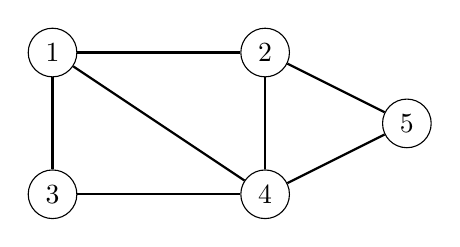
\begin{tikzpicture}[scale=0.9]
\node[draw, circle] (1) at (1,3) {$1$};
\node[draw, circle] (2) at (4,3) {$2$};
\node[draw, circle] (3) at (1,1) {$3$};
\node[draw, circle] (4) at (4,1) {$4$};
\node[draw, circle] (5) at (6,2) {$5$};

\path[draw,thick,-] (1) -- (2);
\path[draw,thick,-] (1) -- (3);
\path[draw,thick,-] (1) -- (4);
\path[draw,thick,-] (3) -- (4);
\path[draw,thick,-] (2) -- (4);
\path[draw,thick,-] (2) -- (5);
\path[draw,thick,-] (4) -- (5);
\end{tikzpicture}
\end{center}
                      
Polku (\textit{path}) on kaaria pitkin kulkeva reitti alkusolmusta
loppusolmuun.
Kuvan verkossa solmusta 1 solmuun 5
johtaa esimerkiksi polku $1 \rightarrow 3 \rightarrow 4 \rightarrow 5$.
Solmun naapuri (\textit{neighbor}) on toinen solmu,
johon solmusta pääsee kaarta pitkin,
ja solmun aste (\textit{degree}) on sen naapurien määrä.
Yllä olevassa verkossa solmun 2
naapurit ovat 1, 4 ja 5,
ja sen aste on 3.

\subsubsection*{Yhtenäisyys}

Verkko on yhtenäinen (\textit{connected}), jos siinä on polku
mistä tahansa solmusta mihin tahansa solmuun.
Esimerkiksi seuraava verkko on yhtenäinen:
\begin{center}
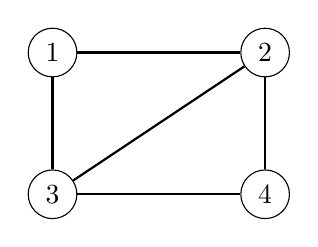
\begin{tikzpicture}[scale=0.9]
\node[draw, circle] (1) at (1,3) {$1$};
\node[draw, circle] (2) at (4,3) {$2$};
\node[draw, circle] (3) at (1,1) {$3$};
\node[draw, circle] (4) at (4,1) {$4$};
\path[draw,thick,-] (1) -- (2);
\path[draw,thick,-] (1) -- (3);
\path[draw,thick,-] (2) -- (3);
\path[draw,thick,-] (3) -- (4);
\path[draw,thick,-] (2) -- (4);
\end{tikzpicture}
\end{center}
Seuraava verkko taas ei ole yhtenäinen,
koska solmu 4 on erillään muista.
\begin{center}
\begin{tikzpicture}[scale=0.9]
\node[draw, circle] (1) at (1,3) {$1$};
\node[draw, circle] (2) at (4,3) {$2$};
\node[draw, circle] (3) at (1,1) {$3$};
\node[draw, circle] (4) at (4,1) {$4$};
\path[draw,thick,-] (1) -- (2);
\path[draw,thick,-] (1) -- (3);
\path[draw,thick,-] (2) -- (3);
%\path[draw,thick,-] (3) -- (4);
%\path[draw,thick,-] (2) -- (4);
\end{tikzpicture}
\end{center}

\subsubsection*{Komponentit}

Verkon yhtenäiset osat muodostavat sen
komponentit (\textit{components}).
Esimerkiksi seuraavassa verkossa on
kolme komponenttia:
$\{1,\,2,\,3\}$,
$\{4,\,5,\,6,\,7\}$ ja
$\{8\}$.
\begin{center}
\begin{tikzpicture}[scale=0.8]
\node[draw, circle] (1) at (1,3) {$1$};
\node[draw, circle] (2) at (4,3) {$2$};
\node[draw, circle] (3) at (1,1) {$3$};

\node[draw, circle] (6) at (6,1) {$6$};
\node[draw, circle] (7) at (9,1) {$7$};
\node[draw, circle] (4) at (6,3) {$4$};
\node[draw, circle] (5) at (9,3) {$5$};

\node[draw, circle] (8) at (11,2) {$8$};

\path[draw,thick,-] (1) -- (2);
\path[draw,thick,-] (2) -- (3);
\path[draw,thick,-] (1) -- (3);
\path[draw,thick,-] (4) -- (5);
\path[draw,thick,-] (5) -- (7);
\path[draw,thick,-] (6) -- (7);
\path[draw,thick,-] (6) -- (4);
\end{tikzpicture}
\end{center}

\subsubsection*{Syklit}

Sykli (\textit{cycle}) on polku, jonka alku- ja loppusolmu
on sama ja jossa ei ole samaa kaarta monta kertaa.
Verkko on syklinen (\textit{cyclic}),
jos siinä on sykli.
Esimerkiksi seuraavassa verkossa
on sykli
$4 \rightarrow 2 \rightarrow 1 \rightarrow 4$.

\begin{center}
\begin{tikzpicture}[scale=0.9]
\node[draw, circle] (1) at (1,3) {$1$};
\node[draw, circle] (2) at (4,3) {$2$};
\node[draw, circle] (3) at (1,1) {$3$};
\node[draw, circle] (4) at (4,1) {$4$};
\node[draw, circle] (5) at (6,2) {$5$};

\path[draw,thick,-] (1) -- (2);
\path[draw,thick,-] (1) -- (3);
\path[draw,thick,-] (1) -- (4);
\path[draw,thick,-] (2) -- (5);
\path[draw,thick,-] (2) -- (4);
\path[draw,thick,-] (4) -- (5);
\end{tikzpicture}
\end{center}

\subsubsection*{Kaarten suunnat}

Verkko on suunnattu (\textit{directed}),
jos verkon kaaria pystyy
kulkemaan vain niiden merkittyyn suuntaan.
Jos taas kaaria voi kulkea kumpaankin
suuntaan, verkko on suuntaamaton (\textit{undirected}).
Esimerkiki seuraava verkko on suunnattu:
\begin{center}
\begin{tikzpicture}[scale=0.9]
\node[draw, circle] (1) at (1,3) {$1$};
\node[draw, circle] (2) at (4,3) {$2$};
\node[draw, circle] (3) at (1,1) {$3$};
\node[draw, circle] (4) at (4,1) {$4$};
\node[draw, circle] (5) at (6,2) {$5$};
\path[draw,thick,->,>=latex] (1) -- (2);
\path[draw,thick,->,>=latex] (2) -- (4);
\path[draw,thick,->,>=latex] (2) -- (5);
\path[draw,thick,->,>=latex] (4) -- (5);
\path[draw,thick,->,>=latex] (4) -- (1);
\path[draw,thick,->,>=latex] (3) -- (1);
\end{tikzpicture}
\end{center}
Tässä verkossa on esimerkiksi polku
$3 \rightarrow 1 \rightarrow 2 \rightarrow 5$,
mutta polkua ei voi kulkea toiseen suuntaan
$5 \rightarrow 2 \rightarrow 1 \rightarrow 3$,
Solmuun 3 ei pääse mistään muusta solmusta,
ja solmusta 5 ei taas pääse mihinkään
muuhun solmuun.

\subsubsection*{Kaarten painot}

Verkko on painotettu (\textit{weighted}),
jos verkon kaariin liittyy painoja.
Tavallinen tulkinta on, että painot kuvaavat
kaarien pituuksia.
Seuraavassa on esimerkki painotetusta verkosta:
\begin{center}
\begin{tikzpicture}[scale=0.9]
\node[draw, circle] (1) at (1,3) {$1$};
\node[draw, circle] (2) at (4,3) {$2$};
\node[draw, circle] (3) at (1,1) {$3$};
\node[draw, circle] (4) at (4,1) {$4$};
\node[draw, circle] (5) at (6,2) {$5$};
\path[draw,thick,-] (1) -- node[font=\small,label=above:5] {} (2);
\path[draw,thick,-] (1) -- node[font=\small,label=left:1] {} (3);
\path[draw,thick,-] (3) -- node[font=\small,label=below:7] {} (4);
\path[draw,thick,-] (2) -- node[font=\small,label=left:4] {} (4);
\path[draw,thick,-] (2) -- node[font=\small,label=above:5] {} (5);
\path[draw,thick,-] (4) -- node[font=\small,label=below:3] {} (5);
\end{tikzpicture}
\end{center}
Polun pituus (\textit{path length}) on
sen kaarten painojen summa.
Esimerkiksi polun $1 \rightarrow 2 \rightarrow 4$
pituus on $5+4=9$ ja polun
$1 \rightarrow 3 \rightarrow 4$ pituus on $1+7=8$.
Jälkimmäinen polku on lyhin polku (\textit{shortest path})
solmusta 1 solmuun 4.

\subsubsection*{Puu}

Puu (\textit{tree})
on yhtenäinen, syklitön ja
suuntaamaton verkko.
Puussa kaarten määrä on aina yhden pienempi
kuin solmujen määrä.
Lisäksi jokaisesta puun solmusta toiseen
on yksikäsitteinen polku.

Esimerkiksi seuraava verkko on puu:
\begin{center}
\begin{tikzpicture}[scale=0.9]
\node[draw, circle] (1) at (0,3) {$2$};
\node[draw, circle] (2) at (2,3) {$3$};
\node[draw, circle] (3) at (0,1) {$5$};
\node[draw, circle] (4) at (2,1) {$6$};
\node[draw, circle] (5) at (4,1) {$7$};
\node[draw, circle] (6) at (-2,3) {$1$};
\node[draw, circle] (7) at (-2,1) {$4$};
\path[draw,thick,-] (1) -- (2);
\path[draw,thick,-] (1) -- (3);
\path[draw,thick,-] (1) -- (4);
\path[draw,thick,-] (2) -- (5);
\path[draw,thick,-] (3) -- (6);
\path[draw,thick,-] (3) -- (7);
\end{tikzpicture}
\end{center}
Puun lehti (\textit{leaf}) on solmu,
josta lähtee vain yksi kaari eli jonka aste on 1.
Yllä olevassa puussa lehtiä ovat solmut 1, 4, 6 ja 7.

Puu esitetään usein juurellisena niin,
että yksi solmuista nostetaan puun juureksi (\textit{root})
ja muut sijoittuvat tasoittain sen alapuolelle.
Esimerkiksi jos äskeisessä verkossa
solmusta 2 tehdään juuri, tulos on tämä:
\begin{center}
\begin{tikzpicture}[scale=0.9]
\node[draw, circle] (1) at (0,3) {$2$};
\node[draw, circle] (2) at (2,1) {$3$};
\node[draw, circle] (3) at (-2,1) {$5$};
\node[draw, circle] (4) at (0,1) {$6$};
\node[draw, circle] (5) at (2,-1) {$7$};
\node[draw, circle] (6) at (-3,-1) {$1$};
\node[draw, circle] (7) at (-1,-1) {$4$};
\path[draw,thick,-] (1) -- (2);
\path[draw,thick,-] (1) -- (3);
\path[draw,thick,-] (1) -- (4);
\path[draw,thick,-] (2) -- (5);
\path[draw,thick,-] (3) -- (6);
\path[draw,thick,-] (3) -- (7);
\end{tikzpicture}
\end{center}
Solmun lapset (\textit{children})
ovat sen alemman tason naapurit
ja solmun vanhempi (\textit{parent}) on ylemmän tason naapuri.
Esimerkiksi kuvan puussa solmun 5
lapset ovat solmut 1 ja 4 ja vanhempi on solmu 2.

\subsubsection*{Kaksijakoisuus}

Verkko on kaksijakoinen (\textit{bipartite}),
jos sen solmut voi värittää kahdella värillä niin,
ettei minkään kaaren molemmissa päissä
ole samanväristä solmua.
Esimerkiksi verkko
\begin{center}
\begin{tikzpicture}[scale=0.9]
\node[draw, circle] (1) at (1,3) {$2$};
\node[draw, circle] (2) at (4,3) {$3$};
\node[draw, circle] (3) at (1,1) {$5$};
\node[draw, circle] (4) at (4,1) {$6$};
\node[draw, circle] (5) at (-2,1) {$4$};
\node[draw, circle] (6) at (-2,3) {$1$};
\path[draw,thick,-] (1) -- (2);
\path[draw,thick,-] (1) -- (3);
\path[draw,thick,-] (3) -- (4);
\path[draw,thick,-] (2) -- (4);
\path[draw,thick,-] (3) -- (6);
\path[draw,thick,-] (5) -- (6);
\end{tikzpicture}
\end{center}
on kaksijakoinen, koska sen voi värittää näin:
\begin{center}
\begin{tikzpicture}[scale=0.9]
\node[draw, circle, fill=blue] (1) at (1,3) {$2$};
\node[draw, circle, fill=red] (2) at (4,3) {$3$};
\node[draw, circle, fill=red] (3) at (1,1) {$5$};
\node[draw, circle, fill=blue] (4) at (4,1) {$6$};
\node[draw, circle, fill=red] (5) at (-2,1) {$4$};
\node[draw, circle, fill=blue] (6) at (-2,3) {$1$};
\path[draw,thick,-] (1) -- (2);
\path[draw,thick,-] (1) -- (3);
\path[draw,thick,-] (3) -- (4);
\path[draw,thick,-] (2) -- (4);
\path[draw,thick,-] (3) -- (6);
\path[draw,thick,-] (5) -- (6);
\end{tikzpicture}
\end{center}
Verkko on kaksijakoinen tarkalleen silloin,
kun siinä ei ole sykliä, jonka osana
on pariton määrä solmuja.

\subsubsection*{Yksinkertaisuus}

Verkko on yksinkertainen (\textit{simple}),
jos mistään solmusta ei ole kaarta itseensä
eikä minkään kahden solmun välillä ole
monta kaarta samaan suuntaan.
Esimerkiksi verkko
\begin{center}
\begin{tikzpicture}[scale=0.9]
\node[draw, circle] (1) at (1,3) {$2$};
\node[draw, circle] (2) at (4,3) {$3$};
\node[draw, circle] (3) at (1,1) {$5$};
\node[draw, circle] (4) at (4,1) {$6$};
\node[draw, circle] (5) at (-2,1) {$4$};
\node[draw, circle] (6) at (-2,3) {$1$};

\path[draw,thick,-] (1) edge [bend right=20] (2);
\path[draw,thick,-] (2) edge [bend right=20] (1);
%\path[draw,thick,-] (1) -- (2);
\path[draw,thick,-] (1) -- (3);
\path[draw,thick,-] (3) -- (4);
\path[draw,thick,-] (2) -- (4);
\path[draw,thick,-] (3) -- (6);
\path[draw,thick,-] (5) -- (6);

\tikzset{every loop/.style={in=135,out=190}}
\path[draw,thick,-] (5) edge [loop left] (5);
\end{tikzpicture}
\end{center}
ei ole yksinkertainen, koska solmusta 4 on kaari itseensä
ja solmujen 2 ja 3 välillä on kaksi kaarta.

\section{Verkko muistissa}

On monia tapoja pitää verkkoa muistissa algoritmissa.
Sopiva tietorakenne riippuu siitä,
kuinka suuri verkko on ja
millä tavoin algoritmi käsittelee sitä.
Seuraavaksi käymme läpi kolme tavallista vaihtoehtoa
käyttäen esimerkkinä seuraavaa verkkoa:
\begin{center}
\begin{tikzpicture}[scale=0.9]
\node[draw, circle] (1) at (1,3) {$1$};
\node[draw, circle] (2) at (1,1) {$4$};
\node[draw, circle] (3) at (3,3) {$2$};
\node[draw, circle] (4) at (5,3) {$3$};
\node[draw, circle] (5) at (3,1) {$5$};
\node[draw, circle] (6) at (5,1) {$6$};

\path[draw,thick,->,>=latex] (1) -- (2);
\path[draw,thick,->,>=latex] (2) -- (3);
\path[draw,thick,->,>=latex] (3) -- (1);
\path[draw,thick,->,>=latex] (3) -- (4);
\path[draw,thick,->,>=latex] (3) -- (5);
\path[draw,thick,->,>=latex] (3) -- (6);
\path[draw,thick,->,>=latex] (6) -- (4);
\path[draw,thick,->,>=latex] (6) -- (5);
\end{tikzpicture}
\end{center}

\subsubsection*{Vieruslistat}

Yleisin tapa pitää verkkoa muistissa
on käyttää vieruslistaesitystä.
Siinä jokaisella solmulla on vieruslista (\textit{adjacency list}),
joka kertoo, mihin solmuihin siitä pääsee suoraan kaarella.
Useimmat verkkoalgoritmit pystyy toteuttamaan tehokkaasti
käyttäen vieruslistaesitystä.

Vieruslistoja varten voi luoda esimerkiksi taulukon vektoreita
\begin{lstlisting}
vector<int> v[N];
\end{lstlisting}
minkä jälkeen kaaret voi lisätä näin:
\begin{lstlisting}
v[1].push_back(4);
v[2].push_back(1);
v[2].push_back(3);
v[2].push_back(5);
v[2].push_back(6);
v[4].push_back(2);
v[6].push_back(3);
v[6].push_back(5);
\end{lstlisting}

Taulukon koko $N$ on valittu niin suureksi,
että taulukossa on oma vieruslista
jokaiselle verkossa esiintyvälle solmulle.

Vieruslistaesityksen avulla voi käydä tehokkaasti
läpi kaikki tietystä solmusta lähtevät kaaret.
Se onnistuu seuraavasti solmulle $s$:
\begin{lstlisting}
for (int i = 0; i < v[s].size(); i++) {
    // käsittele solmu v[s][i]
}
\end{lstlisting}

Jos verkon kaarilla on painot,
vieruslistat voi rakentaa esimerkiksi niin,
että jokainen listan solmu on pari,
jossa on solmun tunnus ja siihen johtavan kaaren paino.
Tällöin verkon määrittelystä tulee
\begin{lstlisting}
vector<pair<int,int>> v[N];
\end{lstlisting}
ja esimerkiksi kaari solmusta 2 solmuun 5 painolla 4 lisätään näin:
\begin{lstlisting}
v[2].push_back({5,4});
\end{lstlisting}

\subsubsection*{Vierusmatriisi}

Vierusmatriisi (\textit{adjacency matrix})
kertoo jokaisesta kaaresta,
onko se mukana verkossa.
Matriisista on tehokasta tarkistaa,
onko kahden solmun välillä kaari,
mutta toisaalta matriisi vie paljon tilaa,
jos verkko on suuri.

Vierusmatriisi on yleensä järkevää tallentaa
taulukkona

\begin{lstlisting}
int v[N][N];
\end{lstlisting}

jossa \texttt{v}[$a$][$b$] on 1,
jos solmusta $a$ on kaari solmuun $b$, ja muuten 0.
Seuraava koodi lisää esimerkin kaaret verkkoon:
\begin{lstlisting}
v[1][4] = 1;
v[2][1] = 1;
v[2][3] = 1;
v[2][5] = 1;
v[2][6] = 1;
v[4][2] = 1;
v[6][3] = 1;
v[6][5] = 1;
\end{lstlisting}

Jos verkko on painotettu, luvun 1 sijasta
vierusmatriisin voi tallentaa luontevasti
kyseisen kaaren painon.

\subsubsection*{Kaarilista}

Kaarilista (\textit{edge list}) sisältää kaikki verkon kaaret.
Kaarilista on hyvä tapa tallentaa verkko,
jos algoritmissa täytyy käydä läpi
kaikki verkon kaaret eikä ole tarvetta
etsiä kaarta alkusolmun perusteella.

Kaarilistan voi tallentaa esimerkiksi vektoriin
\begin{lstlisting}
vector<pair<int,int>> v;
\end{lstlisting}
jossa jokaisessa solmussa on parina kaaren
alku- ja loppusolmu.
Kaaret lisätään listalle näin:

\begin{lstlisting}
v.push_back(make_pair(1,4));
v.push_back(make_pair(2,1));
v.push_back(make_pair(2,3));
v.push_back(make_pair(2,5));
v.push_back(make_pair(2,6));
v.push_back(make_pair(4,2));
v.push_back(make_pair(6,3));
v.push_back(make_pair(6,5));
\end{lstlisting}

Toinen tapa toteuttaa kaarilista
on tallentaa tiedot kaarten alku-
ja loppusolmuista taulukkoihin
seuraavaan tapaan:

\begin{lstlisting}
a[1] = 1; b[1] = 4;
a[2] = 2; b[2] = 1;
a[3] = 2; b[3] = 3;
a[4] = 2; b[4] = 5;
a[5] = 2; b[5] = 6;
a[6] = 4; b[6] = 2;
a[7] = 6; b[7] = 3;
a[8] = 6; b[8] = 5;
\end{lstlisting}
% 
% \subsubsection*{Epäsuora esitys}
% 
% Joskus verkkoa on kätevää käsitellä epäsuoran
% esityksen (\textit{implicit representation}) kautta.
% Tämä tarkoittaa, että muistissa ei ole
% suoraan verkon solmuja ja kaaria
% vaan verkko on kuvattu jollakin
% toisella tavalla.
% 
% Tyypillinen esimerkki epäsuorasta
% verkosta on labyrintti:
% \\
% \begin{center}
% \begin{tikzpicture}[scale=0.7]
% \fill[color=gray] (0,0) rectangle (8,1);
% \fill[color=gray] (0,5) rectangle (8,6);
% \fill[color=gray] (0,0) rectangle (1,6);
% \fill[color=gray] (7,0) rectangle (8,6);
% 
% \fill[color=gray] (2,0) rectangle (3,4);
% \fill[color=gray] (4,2) rectangle (6,4);
% 
% \draw (0,0) grid (8,6);
% 
% \node at (1.5,1.5) {$a$};
% \node at (6.5,3.5) {$b$};
% \end{tikzpicture}
% \end{center}
% ~\\
% Labyrintti vastaa verkkoa,
% jossa jokainen lattiaruutu on solmu
% ja vierekkäisten lattiaruutujen
% välissä on kaari.
% Verkko näyttää tältä:
% \\
% \begin{center}
% \begin{tikzpicture}[scale=0.7]
% \node[draw,circle,minimum size=20pt] (a) at (1,1) {$a$};
% \node[draw,circle,minimum size=20pt] (b) at (1,2.5) {};
% \node[draw,circle,minimum size=20pt] (c) at (1,4) {};
% \node[draw,circle,minimum size=20pt] (d) at (1,5.5) {};
% \node[draw,circle,minimum size=20pt] (e) at (2.5,5.5) {};
% \node[draw,circle,minimum size=20pt] (f) at (4,5.5) {};
% \node[draw,circle,minimum size=20pt] (g) at (5.5,5.5) {};
% \node[draw,circle,minimum size=20pt] (h) at (7,5.5) {};
% \node[draw,circle,minimum size=20pt] (i) at (8.5,5.5) {};
% \node[draw,circle,minimum size=20pt] (j) at (8.5,4) {$b$};
% \node[draw,circle,minimum size=20pt] (k) at (8.5,2.5) {};
% \node[draw,circle,minimum size=20pt] (l) at (8.5,1) {};
% \node[draw,circle,minimum size=20pt] (m) at (7,1) {};
% \node[draw,circle,minimum size=20pt] (n) at (5.5,1) {};
% \node[draw,circle,minimum size=20pt] (o) at (4,1) {};
% \node[draw,circle,minimum size=20pt] (p) at (4,2.5) {};
% \node[draw,circle,minimum size=20pt] (q) at (4,4) {};
% 
% \path[draw,thick,-] (a) -- (b);
% \path[draw,thick,-] (b) -- (c);
% \path[draw,thick,-] (c) -- (d);
% \path[draw,thick,-] (d) -- (e);
% \path[draw,thick,-] (e) -- (f);
% \path[draw,thick,-] (f) -- (g);
% \path[draw,thick,-] (g) -- (h);
% \path[draw,thick,-] (h) -- (i);
% \path[draw,thick,-] (i) -- (j);
% \path[draw,thick,-] (j) -- (k);
% \path[draw,thick,-] (k) -- (l);
% \path[draw,thick,-] (l) -- (m);
% \path[draw,thick,-] (m) -- (n);
% \path[draw,thick,-] (n) -- (o);
% \path[draw,thick,-] (o) -- (p);
% \path[draw,thick,-] (p) -- (q);
% \path[draw,thick,-] (q) -- (f);
% \end{tikzpicture}
% \end{center}
% ~\\
% Kätevä tapa tallentaa labyrintti on luoda taulukko
% merkkijonoista. Jokainen merkkijono vastaa yhtä
% labyrintin riviä:
% \begin{lstlisting}
% s[0] = "########";
% s[1] = "#......#";
% s[2] = "#.#.##b#";
% s[3] = "#.#.##.#";
% s[4] = "#a#....#";
% s[5] = "########";
% \end{lstlisting}

\chapter{Verkon läpikäynti}

Syvyyshaku ja leveyshaku ovat keskeisiä
menetelmiä verkon läpikäyntiin.
Molemmat algoritmit lähtevät liikkeelle
tietystä verkon solmusta ja 
käyvät läpi kaikki solmut,
joihin aloitussolmusta pääsee.
Algoritmien erona on,
missä järjestyksessä ne etenevät verkon solmuja.

\section{Syvyyshaku}

Syvyyshaku (\textit{depth-first search})
on suoraviivainen menetelmä verkon läpikäyntiin.
Syvyyshaku lähtee liikkeelle tietystä
verkon solmusta ja etenee siitä
kaikkiin solmuihin, jotka ovat
saavutettavissa kaaria kulkemalla.

Syvyyshaku etenee verkossa syvyyssuuntaisesti
eli valitsee aina yhden suunnan
ja kulkee eteenpäin niin kauan
kuin vastaan tulee uusia solmuja.
Tämän jälkeen haku perääntyy kokeilemaan
muita suuntia.
Haku pitää kirjaa vierailemistaan solmuista,
jotta se käsittelee kunkin solmun vain kerran.

\subsubsection*{Toiminta}

Tarkastellaan syvyyshaun toimintaa
seuraavassa verkossa:
\begin{center}
\begin{tikzpicture}
\node[draw, circle] (1) at (1,5) {$1$};
\node[draw, circle] (2) at (3,5) {$2$};
\node[draw, circle] (3) at (5,4) {$3$};
\node[draw, circle] (4) at (1,3) {$4$};
\node[draw, circle] (5) at (3,3) {$5$};

\path[draw,thick,-] (1) -- (2);
\path[draw,thick,-] (2) -- (3);
\path[draw,thick,-] (1) -- (4);
\path[draw,thick,-] (3) -- (5);
\path[draw,thick,-] (2) -- (5);
\end{tikzpicture}
\end{center}
Syvyyshaku voi lähteä liikkeelle
mistä tahansa solmusta,
mutta oletetaan nyt,
että haku lähtee liikkeelle solmusta 1.

Solmun 1 naapurit ovat solmut 2 ja 4,
joista haku etenee ensin solmuun 2:
\begin{center}
\begin{tikzpicture}
\node[draw, circle,fill=lightgray] (1) at (1,5) {$1$};
\node[draw, circle,fill=lightgray] (2) at (3,5) {$2$};
\node[draw, circle] (3) at (5,4) {$3$};
\node[draw, circle] (4) at (1,3) {$4$};
\node[draw, circle] (5) at (3,3) {$5$};

\path[draw,thick,-] (1) -- (2);
\path[draw,thick,-] (2) -- (3);
\path[draw,thick,-] (1) -- (4);
\path[draw,thick,-] (3) -- (5);
\path[draw,thick,-] (2) -- (5);

\path[draw=red,thick,->,line width=2pt] (1) -- (2);
\end{tikzpicture}
\end{center}
Tämän jälkeen haku etenee vastaavasti
solmuihin 3 ja 5:
\begin{center}
\begin{tikzpicture}
\node[draw, circle,fill=lightgray] (1) at (1,5) {$1$};
\node[draw, circle,fill=lightgray] (2) at (3,5) {$2$};
\node[draw, circle,fill=lightgray] (3) at (5,4) {$3$};
\node[draw, circle] (4) at (1,3) {$4$};
\node[draw, circle,fill=lightgray] (5) at (3,3) {$5$};

\path[draw,thick,-] (1) -- (2);
\path[draw,thick,-] (2) -- (3);
\path[draw,thick,-] (1) -- (4);
\path[draw,thick,-] (3) -- (5);
\path[draw,thick,-] (2) -- (5);

\path[draw=red,thick,->,line width=2pt] (1) -- (2);
\path[draw=red,thick,->,line width=2pt] (2) -- (3);
\path[draw=red,thick,->,line width=2pt] (3) -- (5);
\end{tikzpicture}
\end{center}
Solmun 5 naapurit ovat 2 ja 3,
mutta haku on käynyt jo molemmissa,
joten on aika peruuttaa taaksepäin.
Myös solmujen 3 ja 2 naapurit on käyty,
joten haku peruuttaa solmuun 1 asti.
Siitä lähtee kaari, josta pääsee
solmuun 4:
\begin{center}
\begin{tikzpicture}
\node[draw, circle,fill=lightgray] (1) at (1,5) {$1$};
\node[draw, circle,fill=lightgray] (2) at (3,5) {$2$};
\node[draw, circle,fill=lightgray] (3) at (5,4) {$3$};
\node[draw, circle,fill=lightgray] (4) at (1,3) {$4$};
\node[draw, circle,fill=lightgray] (5) at (3,3) {$5$};

\path[draw,thick,-] (1) -- (2);
\path[draw,thick,-] (2) -- (3);
\path[draw,thick,-] (1) -- (4);
\path[draw,thick,-] (3) -- (5);
\path[draw,thick,-] (2) -- (5);

\path[draw=red,thick,->,line width=2pt] (1) -- (4);
\end{tikzpicture}
\end{center}
Tämän jälkeen haku päättyy,
koska se on käynyt kaikissa solmuissa.

Syvyyshaun aikavaativuus on $O(n+m)$,
missä $n$ on solmujen määrä ja $m$ on kaarten määrä,
koska haku käsittelee kerran jokaisen solmun ja kaaren.

\subsubsection*{Toteutus}

Syvyyshaku on yleensä mukavinta toteuttaa
rekursiolla.
Seuraava funktio \texttt{dfs}
suorittaa syvyyshaun sille parametrina
annetusta solmusta lähtien.
Funktio olettaa, että
verkko on tallennettu vieruslistoina
taulukkoon
\begin{lstlisting}
vector<int> v[N];
\end{lstlisting}
ja pitää lisäksi yllä taulukkoa
\begin{lstlisting}
int z[N];
\end{lstlisting}
joka kertoo, missä solmuissa haku on käynyt.
Alussa taulukon jokainen arvo on 0,
ja kun haku saapuu solmuun $s$,
sen kohdalle merkitään luku 1.
Funktion toteutus on seuraavanlainen:
\begin{lstlisting}
void dfs(int s) {
    if (z[s]) return;
    z[s] = 1;
    // solmun s käsittely tähän
    for (int i = 0; i < v[s].size(); i++) {
        dfs(v[s][i]);
    }
}
\end{lstlisting}

\section{Leveyshaku}

Leveyshaku (\textit{breadth-first search})
käy solmut läpi järjestyksessä sen mukaan,
kuinka kaukana ne ovat aloitussolmusta.
Niinpä leveyshaun avulla pystyy laskemaan
etäisyyden aloitussolmusta kaikkiin
muihin solmuihin.
Leveyshaku on kuitenkin vaikeampi
toteuttaa kuin syvyyshaku.

Leveyshakua voi ajatella niin,
että se käy solmuja läpi kerros kerrallaan.
Ensin haku käy läpi solmut,
joihin pääsee yhdellä kaarella
alkusolmusta.
Tämän jälkeen vuorossa ovat
solmut, joihin pääsee kahdella
kaarella alkusolmusta jne.
Sama jatkuu, kunnes uusia käsiteltäviä
solmuja ei enää ole.

\subsubsection*{Toiminta}

Tarkastellaan leveyshaun toimintaa
seuraavassa verkossa:

\begin{center}
\begin{tikzpicture}
\node[draw, circle] (1) at (1,5) {$1$};
\node[draw, circle] (2) at (3,5) {$2$};
\node[draw, circle] (3) at (5,5) {$3$};
\node[draw, circle] (4) at (1,3) {$4$};
\node[draw, circle] (5) at (3,3) {$5$};
\node[draw, circle] (6) at (5,3) {$6$};


\path[draw,thick,-] (1) -- (2);
\path[draw,thick,-] (2) -- (3);
\path[draw,thick,-] (1) -- (4);
\path[draw,thick,-] (3) -- (6);
\path[draw,thick,-] (2) -- (5);
\path[draw,thick,-] (5) -- (6);
\end{tikzpicture}
\end{center}
Oletetaan jälleen,
että haku alkaa solmusta 1.
Haku etenee ensin kaikkiin solmuihin,
joihin pääsee alkusolmusta:
\\
\begin{center}
\begin{tikzpicture}
\node[draw, circle,fill=lightgray] (1) at (1,5) {$1$};
\node[draw, circle,fill=lightgray] (2) at (3,5) {$2$};
\node[draw, circle] (3) at (5,5) {$3$};
\node[draw, circle,fill=lightgray] (4) at (1,3) {$4$};
\node[draw, circle] (5) at (3,3) {$5$};
\node[draw, circle] (6) at (5,3) {$6$};

\path[draw,thick,-] (1) -- (2);
\path[draw,thick,-] (2) -- (3);
\path[draw,thick,-] (1) -- (4);
\path[draw,thick,-] (3) -- (6);
\path[draw,thick,-] (2) -- (5);
\path[draw,thick,-] (5) -- (6);

\path[draw,thick,-] (1) -- (2);
\path[draw,thick,-] (2) -- (3);
\path[draw,thick,-] (1) -- (4);
\path[draw,thick,-] (2) -- (5);

\path[draw=red,thick,->,line width=2pt] (1) -- (2);
\path[draw=red,thick,->,line width=2pt] (1) -- (4);
\end{tikzpicture}
\end{center}
Seuraavaksi haku etenee solmuihin 3 ja 5:
\\
\begin{center}
\begin{tikzpicture}
\node[draw, circle,fill=lightgray] (1) at (1,5) {$1$};
\node[draw, circle,fill=lightgray] (2) at (3,5) {$2$};
\node[draw, circle,fill=lightgray] (3) at (5,5) {$3$};
\node[draw, circle,fill=lightgray] (4) at (1,3) {$4$};
\node[draw, circle,fill=lightgray] (5) at (3,3) {$5$};
\node[draw, circle] (6) at (5,3) {$6$};

\path[draw,thick,-] (1) -- (2);
\path[draw,thick,-] (2) -- (3);
\path[draw,thick,-] (1) -- (4);
\path[draw,thick,-] (3) -- (6);
\path[draw,thick,-] (2) -- (5);
\path[draw,thick,-] (5) -- (6);

\path[draw,thick,-] (1) -- (2);
\path[draw,thick,-] (2) -- (3);
\path[draw,thick,-] (1) -- (4);
\path[draw,thick,-] (2) -- (5);

\path[draw=red,thick,->,line width=2pt] (2) -- (3);
\path[draw=red,thick,->,line width=2pt] (2) -- (5);
\end{tikzpicture}
\end{center}
Viimeisenä haku etenee solmuun 6:
\\
\begin{center}
\begin{tikzpicture}
\node[draw, circle,fill=lightgray] (1) at (1,5) {$1$};
\node[draw, circle,fill=lightgray] (2) at (3,5) {$2$};
\node[draw, circle,fill=lightgray] (3) at (5,5) {$3$};
\node[draw, circle,fill=lightgray] (4) at (1,3) {$4$};
\node[draw, circle,fill=lightgray] (5) at (3,3) {$5$};
\node[draw, circle,fill=lightgray] (6) at (5,3) {$6$};

\path[draw,thick,-] (1) -- (2);
\path[draw,thick,-] (2) -- (3);
\path[draw,thick,-] (1) -- (4);
\path[draw,thick,-] (3) -- (6);
\path[draw,thick,-] (2) -- (5);
\path[draw,thick,-] (5) -- (6);

\path[draw,thick,-] (1) -- (2);
\path[draw,thick,-] (2) -- (3);
\path[draw,thick,-] (1) -- (4);
\path[draw,thick,-] (2) -- (5);

\path[draw=red,thick,->,line width=2pt] (3) -- (6);
\path[draw=red,thick,->,line width=2pt] (5) -- (6);
\end{tikzpicture}
\end{center}
Leveyshaun tuloksena selviää etäisyys
kuhunkin verkon solmuun alkusolmusta.
Etäisyys on sama kuin kerros,
jossa solmu käsiteltiin haun aikana:

\begin{tabular}{ll}
\\
solmu & etäisyys \\
\hline
1 & 0 \\
2 & 1 \\
3 & 2 \\
4 & 1 \\
5 & 2 \\
6 & 3 \\
\\
\end{tabular}

Leveyshaun aikavaativuus on syvyyshaun tavoin $O(n+m)$,
missä $n$ on solmujen määrä ja $m$ on kaarten määrä.

\subsubsection*{Toteutus}

Leveyshaun toteutus on syvyyshakua monimutkaisempi,
koska haku käy läpi solmuja verkon eri
puolilta niiden etäisyyden mukaan.
Tyypillinen toteutus on pitää yllä jonoa
käsiteltävistä solmuista.
Joka askeleella otetaan käsittelyyn seuraava
solmu jonosta ja uudet solmut lisätään
jonon perälle.

Seuraava koodi toteuttaa leveyshaun
solmusta $s$ lähtien.
Koodi olettaa, että verkko on tallennettu
vieruslistoina, ja pitää yllä jonoa
\begin{lstlisting}
queue<int> q;
\end{lstlisting}
joka sisältää solmut käsittelyjärjestyksessä.
Koodi lisää aina uudet vastaan tulevat solmut
jonon perään ja ottaa seuraavaksi käsiteltävän
solmun jonon alusta,
minkä ansiosta solmut käsitellään tasoittain
alkusolmusta lähtien.

Lisäksi koodi käyttää taulukoita
\begin{lstlisting}
int z[N], e[N];
\end{lstlisting}
niin, että taulukko \texttt{z} sisältää tiedon,
missä solmuissa haku on käynyt,
ja taulukkoon \texttt{e} lasketaan lyhin
etäisyys alkusolmusta kaikkiin verkon solmuihin.
Toteutuksesta tulee seuraavanlainen:
\begin{lstlisting}
q.push(s);
z[s] = 1; e[s] = 0;
while (!q.empty()) {
    int s = q.front(); q.pop();
    // solmun s käsittely tähän     
    for (int i = 0; i < v[s].size(); i++) {
        int u = v[s][i];
        if (z[u]) continue;
        z[u] = 1; e[u] = e[s]+1;
        q.push(u);
    }
}
\end{lstlisting}

\section{Sovelluksia}

Verkon läpikäyntien avulla
saa selville monia asioita
verkon rakenteesta.
Seuraavissa sovelluksissa
voi käyttää joko
syvyyshakua tai leveyshakua,
mutta syvyyshaku
on käytännössä parempi valinta,
koska sen toteutus on helpompi.

\subsubsection{Yhtenäisyys}

Verkko on yhtenäinen,
jos mistä tahansa solmuista
pääsee kaikkiin muihin solmuihin.
Niinpä verkon yhtenäisyys selviää
aloittamalla läpikäynti
jostakin verkon solmusta ja
tarkastamalla, pääseekö siitä kaikkiin solmuihin.
Jos kaikki solmut
tulevat vastaan läpikäynnin aikana,
niin verkko on yhtenäinen.

\subsubsection{Komponentit}

Jos verkko ei ole yhtenäinen,
se muodostuu useammasta komponentista.
Kaikki tiettyyn komponenttiin kuuluvat
solmut löytyvät aloittamalla
läpikäynti jostakin komponentin solmusta.

Verkon komponentit saa selville
käymällä läpi verkon solmut ja
pitämällä kirjaa komponenteista.
Jos solmu ei kuulu vielä
komponenttiin, se aloittaa uuden
komponentin, johon kuuluvat kaikki
solmut, joihin solmusta pääsee.

\subsubsection{Syklin etsiminen}

Suuntaamaton verkko sisältää syklin,
jos verkon läpikäynnin aikana tulee vastaan
solmu, jossa on käyty jo aiemmin,
ja tämä solmu on jokin muu kuin se solmu,
jonka kautta nykyiseen solmuun tultiin.

Syklin olemassaolon voi myös päätellä
komponentin koosta. Jos komponentin
kaarten määrä on yhtä pienempi kuin
solmujen määrä, komponentissa ei ole sykliä,
ja jos kaarten määrä on tätä suurempi,
komponentissa on sykli.

\subsubsection{Kaksijakoisuus}

Verkko on kaksijakoinen,
jos sen solmut voi värittää
kahdella värillä
niin, että kahta samanväristä
solmua ei ole vierekkäin.
Kaksijakoisuus on yllättävän
helppoa selvittää
verkon läpikäynnin avulla.

Ideana on värittää alkusolmu
siniseksi, sen kaikki naapurit
punaiseksi, niiden kaikki naapurit
siniseksi, jne.
Jos jossain vaiheessa
ilmenee ristiriita
(saman solmun tulisi olla sekä
sininen että punainen),
verkko ei ole kaksijakoinen.
Muuten verkko on kaksijakoinen
ja yksi väritys on muodostunut.

Tämä algoritmi toimii,
koska kun värejä on vain kaksi,
ensimmäisen solmun värin valinta
määrittää kaikkien muiden
samassa komponentissa olevien
solmujen värin.
Ei ole merkitystä,
kumman värin ensimmäinen
solmu saa.

Yleensä ottaen on vaikea ongelma
selvittää, voiko verkon solmuja
värittää $k$ värillä niin,
ettei missään kohtaa ole vierekkäin
kahta samanväristä solmua.
Edes tapaukseen $k=3$ ei tunneta
mitään tehokasta algoritmia.

\section{Labyrintin käsittely}

Labyrintti on ruudukko, joka muodostuu lattia- ja seinäruuduista,
ja labyrintissa on sallittua kulkea lattiaruutuja pitkin.
Labyrinttia
\begin{center}
\begin{tikzpicture}[scale=0.7]
\fill[color=gray] (0,0) rectangle (8,1);
\fill[color=gray] (0,5) rectangle (8,6);
\fill[color=gray] (0,0) rectangle (1,6);
\fill[color=gray] (7,0) rectangle (8,6);

\fill[color=gray] (2,0) rectangle (3,4);
\fill[color=gray] (4,2) rectangle (6,4);

\draw (0,0) grid (8,6);

\node at (1.5,1.5) {$a$};
\node at (6.5,3.5) {$b$};
\end{tikzpicture}
\end{center}
vastaa luontevasti verkko
\begin{center}
\begin{tikzpicture}[scale=0.7]
\node[draw,circle,minimum size=20pt] (a) at (1,1) {$a$};
\node[draw,circle,minimum size=20pt] (b) at (1,2.5) {};
\node[draw,circle,minimum size=20pt] (c) at (1,4) {};
\node[draw,circle,minimum size=20pt] (d) at (1,5.5) {};
\node[draw,circle,minimum size=20pt] (e) at (2.5,5.5) {};
\node[draw,circle,minimum size=20pt] (f) at (4,5.5) {};
\node[draw,circle,minimum size=20pt] (g) at (5.5,5.5) {};
\node[draw,circle,minimum size=20pt] (h) at (7,5.5) {};
\node[draw,circle,minimum size=20pt] (i) at (8.5,5.5) {};
\node[draw,circle,minimum size=20pt] (j) at (8.5,4) {$b$};
\node[draw,circle,minimum size=20pt] (k) at (8.5,2.5) {};
\node[draw,circle,minimum size=20pt] (l) at (8.5,1) {};
\node[draw,circle,minimum size=20pt] (m) at (7,1) {};
\node[draw,circle,minimum size=20pt] (n) at (5.5,1) {};
\node[draw,circle,minimum size=20pt] (o) at (4,1) {};
\node[draw,circle,minimum size=20pt] (p) at (4,2.5) {};
\node[draw,circle,minimum size=20pt] (q) at (4,4) {};

\path[draw,thick,-] (a) -- (b);
\path[draw,thick,-] (b) -- (c);
\path[draw,thick,-] (c) -- (d);
\path[draw,thick,-] (d) -- (e);
\path[draw,thick,-] (e) -- (f);
\path[draw,thick,-] (f) -- (g);
\path[draw,thick,-] (g) -- (h);
\path[draw,thick,-] (h) -- (i);
\path[draw,thick,-] (i) -- (j);
\path[draw,thick,-] (j) -- (k);
\path[draw,thick,-] (k) -- (l);
\path[draw,thick,-] (l) -- (m);
\path[draw,thick,-] (m) -- (n);
\path[draw,thick,-] (n) -- (o);
\path[draw,thick,-] (o) -- (p);
\path[draw,thick,-] (p) -- (q);
\path[draw,thick,-] (q) -- (f);
\end{tikzpicture}
\end{center}
jossa verkon solmuja ovat labyrintin lattiaruudut
ja solmujen välillä on kaari, jos lattiaruudusta
toiseen pääsee kulkemaan yhdellä askeleella.
Niinpä erilaiset labyrinttiin liittyvät ongelmat
palautuvat verkko-ongelmiksi.

Esimerkiksi syvyyshaulla pystyy selvittämään,
onko ruudusta $a$ reittiä ruutuun $b$
ja leveyshaku kertoo lisäksi,
mikä on pienin mahdollinen askelten määrä reitillä.
Samoin voi esimerkiksi vaikkapa, kuinka monta
toisistaan erillistä huonetta labyrintissa on
sekä kuinka monta ruutua huoneissa on.

Labyrintin tapauksessa ei kannata muodostaa erikseen
verkkoa, vaan syvyyshaun ja leveyshaun voi toteuttaa
suoraan labyrintin ruudukkoon.
\chapter{Lyhimmät polut}

Lyhimmän polun etsiminen alkusolmusta loppusolmuun
on keskeinen verkko-ongelma, joka esiintyy usein
käytännön tilanteissa.
Esimerkiksi tieverkostossa
tyypillinen ongelma on selvittää,
mikä on lyhin reitti kahden kaupungin välillä,
kun tiedossa ovat kaupunkien väliset tiet ja niiden pituudet.

Jos verkon kaarilla ei ole painoja,
polun pituus on sama kuin kaarten
määrä polulla, jolloin lyhimmän polun
voi etsiä leveyshaulla.
Tässä luvussa keskitymme kuitenkin
tapaukseen, jossa kaarilla on painot.
Tällöin lyhimpien polkujen etsimiseen
tarvitaan kehittyneempiä algoritmeja.

\section{Bellman-Fordin algoritmi}

Bellman-Fordin algoritmi etsii
lyhimmän polun alkusolmusta
kaikkiin muihin verkon solmuihin.
Algoritmi on helppo toteuttaa, ja
sitä voi käyttää kaikenlaisissa verkoissa.
Algoritmi pystyy myös tunnistamaan,
onko verkossa sykliä,
jonka pituus on negatiivinen.

Algoritmi pitää yllä etäisyysarvioita
alkusolmusta kaikkiin muihin verkon solmuihin.
Alussa alkusolmun etäisyysarvio on 0
ja muiden solmujen etäisyys\-arvio on ääretön.
Algoritmi parantaa arvioita
etsimällä verkosta kaaria,
jotka lyhentävät polkuja,
kunnes mitään arviota ei voi enää parantaa.

\subsubsection{Toiminta}

Tarkastellaan Bellman-Fordin
algoritmin toimintaa seuraavassa verkossa:
\begin{center}
\begin{tikzpicture}
\node[draw, circle] (1) at (1,3) {1};
\node[draw, circle] (2) at (4,3) {2};
\node[draw, circle] (3) at (1,1) {3};
\node[draw, circle] (4) at (4,1) {4};
\node[draw, circle] (5) at (6,2) {5};
\node[color=red] at (1,3+0.55) {$0$};
\node[color=red] at (4,3+0.55) {$\infty$};
\node[color=red] at (1,1-0.55) {$\infty$};
\node[color=red] at (4,1-0.55) {$\infty$};
\node[color=red] at (6,2-0.55) {$\infty$};
\path[draw,thick,-] (1) -- node[font=\small,label=above:2] {} (2);
\path[draw,thick,-] (1) -- node[font=\small,label=left:3] {} (3);
\path[draw,thick,-] (3) -- node[font=\small,label=below:$-2$] {} (4);
\path[draw,thick,-] (2) -- node[font=\small,label=left:3] {} (4);
\path[draw,thick,-] (2) -- node[font=\small,label=above:5] {} (5);
\path[draw,thick,-] (4) -- node[font=\small,label=below:2] {} (5);
\path[draw,thick,-] (1) -- node[font=\small,label=above:7] {} (4);
\end{tikzpicture}
\end{center}
Verkon jokaiseen solmun viereen on merkitty etäisyysarvio.
Alussa alkusolmun etäisyysarvio on 0
ja muiden solmujen etäisyysarvio on
ääretön ($\infty$).

Algoritmin etsii verkosta kaaria,
jotka parantavat etäisyysarvioita.
Aluksi kaikki solmusta 0 lähtevät kaaret
parantavat arvioita:
\begin{center}
\begin{tikzpicture}
\node[draw, circle] (1) at (1,3) {1};
\node[draw, circle] (2) at (4,3) {2};
\node[draw, circle] (3) at (1,1) {3};
\node[draw, circle] (4) at (4,1) {4};
\node[draw, circle] (5) at (6,2) {5};
\node[color=red] at (1,3+0.55) {$0$};
\node[color=red] at (4,3+0.55) {$2$};
\node[color=red] at (1,1-0.55) {$3$};
\node[color=red] at (4,1-0.55) {$7$};
\node[color=red] at (6,2-0.55) {$\infty$};
\path[draw,thick,-] (1) -- node[font=\small,label=above:2] {} (2);
\path[draw,thick,-] (1) -- node[font=\small,label=left:3] {} (3);
\path[draw,thick,-] (3) -- node[font=\small,label=below:$-2$] {} (4);
\path[draw,thick,-] (2) -- node[font=\small,label=left:3] {} (4);
\path[draw,thick,-] (2) -- node[font=\small,label=above:5] {} (5);
\path[draw,thick,-] (4) -- node[font=\small,label=below:2] {} (5);
\path[draw,thick,-] (1) -- node[font=\small,label=above:7] {} (4);

\path[draw=red,thick,->,line width=2pt] (1) -- (2);
\path[draw=red,thick,->,line width=2pt] (1) -- (3);
\path[draw=red,thick,->,line width=2pt] (1) -- (4);
\end{tikzpicture}
\end{center}

Sitten kaaret $2 \rightarrow 5$ ja $3 \rightarrow 4$
parantavat arvioita:

\begin{center}
\begin{tikzpicture}
\node[draw, circle] (1) at (1,3) {1};
\node[draw, circle] (2) at (4,3) {2};
\node[draw, circle] (3) at (1,1) {3};
\node[draw, circle] (4) at (4,1) {4};
\node[draw, circle] (5) at (6,2) {5};
\node[color=red] at (1,3+0.55) {$0$};
\node[color=red] at (4,3+0.55) {$2$};
\node[color=red] at (1,1-0.55) {$3$};
\node[color=red] at (4,1-0.55) {$1$};
\node[color=red] at (6,2-0.55) {$7$};
\path[draw,thick,-] (1) -- node[font=\small,label=above:2] {} (2);
\path[draw,thick,-] (1) -- node[font=\small,label=left:3] {} (3);
\path[draw,thick,-] (3) -- node[font=\small,label=below:$-2$] {} (4);
\path[draw,thick,-] (2) -- node[font=\small,label=left:3] {} (4);
\path[draw,thick,-] (2) -- node[font=\small,label=above:5] {} (5);
\path[draw,thick,-] (4) -- node[font=\small,label=below:2] {} (5);
\path[draw,thick,-] (1) -- node[font=\small,label=above:7] {} (4);

\path[draw=red,thick,->,line width=2pt] (2) -- (5);
\path[draw=red,thick,->,line width=2pt] (3) -- (4);
\end{tikzpicture}
\end{center}

Lopuksi tulee vielä yksi parannus:

\begin{center}
\begin{tikzpicture}
\node[draw, circle] (1) at (1,3) {1};
\node[draw, circle] (2) at (4,3) {2};
\node[draw, circle] (3) at (1,1) {3};
\node[draw, circle] (4) at (4,1) {4};
\node[draw, circle] (5) at (6,2) {5};
\node[color=red] at (1,3+0.55) {$0$};
\node[color=red] at (4,3+0.55) {$2$};
\node[color=red] at (1,1-0.55) {$3$};
\node[color=red] at (4,1-0.55) {$1$};
\node[color=red] at (6,2-0.55) {$3$};
\path[draw,thick,-] (1) -- node[font=\small,label=above:2] {} (2);
\path[draw,thick,-] (1) -- node[font=\small,label=left:3] {} (3);
\path[draw,thick,-] (3) -- node[font=\small,label=below:$-2$] {} (4);
\path[draw,thick,-] (2) -- node[font=\small,label=left:3] {} (4);
\path[draw,thick,-] (2) -- node[font=\small,label=above:5] {} (5);
\path[draw,thick,-] (4) -- node[font=\small,label=below:2] {} (5);
\path[draw,thick,-] (1) -- node[font=\small,label=above:7] {} (4);

\path[draw=red,thick,->,line width=2pt] (4) -- (5);
\end{tikzpicture}
\end{center}

Tämän jälkeen mikään kaari
ei paranna etäisyysarvioita.
Tämä tarkoittaa, että etäisyydet
ovat lopulliset, eli joka solmussa
on nyt pienin etäisyys alkusolmusta
kyseiseen solmuun.

Esimerkiksi pienin etäisyys 3
solmusta 1 solmuun 5 toteutuu käyttämällä
seuraavaa reittiä:

\begin{center}
\begin{tikzpicture}
\node[draw, circle] (1) at (1,3) {1};
\node[draw, circle] (2) at (4,3) {2};
\node[draw, circle] (3) at (1,1) {3};
\node[draw, circle] (4) at (4,1) {4};
\node[draw, circle] (5) at (6,2) {5};
\node[color=red] at (1,3+0.55) {$0$};
\node[color=red] at (4,3+0.55) {$2$};
\node[color=red] at (1,1-0.55) {$3$};
\node[color=red] at (4,1-0.55) {$1$};
\node[color=red] at (6,2-0.55) {$3$};
\path[draw,thick,-] (1) -- node[font=\small,label=above:2] {} (2);
\path[draw,thick,-] (1) -- node[font=\small,label=left:3] {} (3);
\path[draw,thick,-] (3) -- node[font=\small,label=below:$-2$] {} (4);
\path[draw,thick,-] (2) -- node[font=\small,label=left:3] {} (4);
\path[draw,thick,-] (2) -- node[font=\small,label=above:5] {} (5);
\path[draw,thick,-] (4) -- node[font=\small,label=below:2] {} (5);
\path[draw,thick,-] (1) -- node[font=\small,label=above:7] {} (4);

\path[draw=red,thick,->,line width=2pt] (1) -- (3);
\path[draw=red,thick,->,line width=2pt] (3) -- (4);
\path[draw=red,thick,->,line width=2pt] (4) -- (5);
\end{tikzpicture}
\end{center}

\subsubsection{Toteutus}

Seuraava Bellman-Fordin algoritmin toteutus
tunnetaan nimellä SPFA-al\-go\-rit\-mi
(\textit{Shortest Path Faster Algorithm}).
Se pitää yllä jonoa solmuista,
joiden kautta kulkevaa polkua saattaa pystyä lyhentämään,
ja valitsee aina seuraavan käsiteltävän solmun
jonon alusta.

Koodi olettaa, että verkko on tallennettuna
vieruslistoina taulukossa \texttt{v}.
Jokainen vieruslista muodostuu pareista,
joissa on ensin kaaren kohdesolmu ja sitten kaaren paino.
Koodi laskee taulukkoon \texttt{e} lyhimmän etäisyyden
alkusolmusta $x$ kaikkiin muihin solmuihin.

Jono \texttt{q} sisältää käsiteltävät verkon solmut:
\begin{lstlisting}
queue<int> q;
\end{lstlisting}

Alussa jonoon lisätään vain solmu $x$.
Koodi käy läpi jonon solmuja ja yrittää lyhentää
polkuja niistä lähtevillä kaarilla.
Aina kun polun pituus lyhenee
kaaren $a \rightarrow b$ ansiosta,
jonoon lisätään solmu $b$.

\begin{lstlisting}
for (int i = 1; i <= n; i++) e[i] = 1e9;
e[x] = 0;
q.push(x);
while (!q.empty()) {
    auto s = q.front(); q.pop();
    for (auto u : v[s]) {
        if (e[s]+u.second < e[u.first]) {
            e[u.first] = e[s]+u.second;
            q.push(u.first);
        }
    }
}
\end{lstlisting}
Algoritmi pysähtyy aina viimeistään $O(nm)$
parannuksen jälkeen, jos verkossa ei ole negatiivista sykliä.
Tämä johtuu siitä, että jokaisessa lyhimmässä polussa
on $O(m)$ kaarta

\subsubsection{Negatiivinen sykli}

Bellman-Fordin algoritmin avulla voi myös tarkastaa,
onko verkossa sykliä,
jonka pituus on negatiivinen.
Esimerkiksi verkossa

\begin{center}
\begin{tikzpicture}
\node[draw, circle] (1) at (0,0) {$1$};
\node[draw, circle] (2) at (2,1) {$2$};
\node[draw, circle] (3) at (2,-1) {$3$};
\node[draw, circle] (4) at (4,0) {$4$};

\path[draw,thick,-] (1) -- node[font=\small,label=above:$3$] {} (2);
\path[draw,thick,-] (2) -- node[font=\small,label=above:$1$] {} (4);
\path[draw,thick,-] (1) -- node[font=\small,label=below:$5$] {} (3);
\path[draw,thick,-] (3) -- node[font=\small,label=below:$-7$] {} (4);
\path[draw,thick,-] (2) -- node[font=\small,label=right:$2$] {} (3);
\end{tikzpicture}
\end{center}
\noindent
on negatiivinen sykli $2 \rightarrow 3 \rightarrow 4 \rightarrow 2$,
jonka pituus on $-4$.

Jos verkossa on negatiivinen sykli,
sen kautta kulkevaa polkua voi lyhentää äärettömästi
toistamalla negatiivista sykliä uudestaan ja uudestaan,
minkä vuoksi lyhimmän polun käsite ei ole mielekäs.

Negatiivisen syklin voi tunnistaa
Bellman-Fordin algoritmilla
alustamalla ensin kaikki etäisyysarviot nolliksi
ja suorittamalla sitten
algoritmia $n$ kierrosta.
Jos viimeinen kierros parantaa jotain
etäisyysarviota, verkossa on negatiivinen sykli.
Huomaa, että tässä mikään solmuista ei ole alkusolmu
ja algoritmi etsii negatiivista sykliä koko verkon alueelta.

\section{Dijkstran algoritmi}

Dijkstran algoritmi etsii Bellman-Fordin
algoritmin tavoin lyhimmät polut
alkusolmusta kaikkiin muihin solmuihin.
Dijkstran algoritmi on tehokkaampi kuin
Bellman-Fordin algoritmi,
minkä ansiosta se soveltuu suurten
verkkojen käsittelyyn.
Algoritmi vaatii kuitenkin,
ettei verkossa ole negatiivisia kaaria.

Dijkstran algoritmi vastaa
Bellman-Fordin algoritmia siinä,
että se pitää
yllä etäisyysarvioita solmuihin
ja parantaa niitä algoritmin aikana.
Algoritmin tehokkuus perustuu
siihen, että sen riittää käydä läpi
verkon kaaret vain kerran
hyödyntäen tietoa,
ettei verkossa ole negatiivisia kaaria.

\subsubsection{Toiminta}

Tarkastellaan Dijkstran algoritmin toimintaa
seuraavassa verkossa:
\begin{center}
\begin{tikzpicture}
\node[draw, circle] (1) at (1,3) {$\infty$};
\node[draw, circle] (2) at (4,3) {$\infty$};
\node[draw, circle] (3) at (1,1) {$\infty$};
\node[draw, circle] (4) at (4,1) {$0$};
\node[draw, circle] (5) at (6,2) {$\infty$};

\path[draw,thick,-] (1) -- node[font=\small,label=above:6] {} (2);
\path[draw,thick,-] (1) -- node[font=\small,label=left:2] {} (3);
\path[draw,thick,-] (3) -- node[font=\small,label=below:5] {} (4);
\path[draw,thick,-] (2) -- node[font=\small,label=left:9] {} (4);
\path[draw,thick,-] (2) -- node[font=\small,label=above:2] {} (5);
\path[draw,thick,-] (4) -- node[font=\small,label=below:1] {} (5);
\end{tikzpicture}
\end{center}
Bellman-Fordin algoritmin tavoin
alkusolmun etäisyysarvio on 0
ja kaikissa muissa solmuissa etäisyysarvio
on aluksi $\infty$.

Dijkstran algoritmi
ottaa joka askeleella käsittelyyn
sellaisen solmun,
jota ei ole vielä käsitelty
ja jonka etäisyysarvio on
mahdollisimman pieni.
Alussa tällainen solmu on alkusolmu,
jonka etäisyysarvio on 0.

Kun solmu tulee käsittelyyn,
algoritmi käy läpi kaikki
siitä lähtevät kaaret ja
parantaa etäisyysarvioita
niiden avulla:
\begin{center}
\begin{tikzpicture}
\node[draw, circle] (1) at (1,3) {$\infty$};
\node[draw, circle] (2) at (4,3) {$9$};
\node[draw, circle] (3) at (1,1) {$5$};
\node[draw, circle, fill=lightgray] (4) at (4,1) {$0$};
\node[draw, circle] (5) at (6,2) {$1$};

\path[draw,thick,-] (1) -- node[font=\small,label=above:6] {} (2);
\path[draw,thick,-] (1) -- node[font=\small,label=left:2] {} (3);
\path[draw,thick,-] (3) -- node[font=\small,label=below:5] {} (4);
\path[draw,thick,-] (2) -- node[font=\small,label=left:9] {} (4);
\path[draw,thick,-] (2) -- node[font=\small,label=above:2] {} (5);
\path[draw,thick,-] (4) -- node[font=\small,label=below:1] {} (5);

\path[draw=red,thick,->,line width=2pt] (4) -- (2);
\path[draw=red,thick,->,line width=2pt] (4) -- (3);
\path[draw=red,thick,->,line width=2pt] (4) -- (5);
\end{tikzpicture}
\end{center}
Alkusolmun käsittely paransi etäisyysarvioita
kolmen muuhun solmuun,
joiden uudet etäisyydet ovat nyt 1, 5 ja 9.

\begin{samepage}
Seuraavaksi käsittelyyn tulee solmu,
jonka etäisyys on 1:

\begin{center}
\begin{tikzpicture}
\node[draw, circle] (1) at (1,3) {$\infty$};
\node[draw, circle] (2) at (4,3) {$3$};
\node[draw, circle] (3) at (1,1) {$5$};
\node[draw, circle, fill=lightgray] (4) at (4,1) {$0$};
\node[draw, circle, fill=lightgray] (5) at (6,2) {$1$};

\path[draw,thick,-] (1) -- node[font=\small,label=above:6] {} (2);
\path[draw,thick,-] (1) -- node[font=\small,label=left:2] {} (3);
\path[draw,thick,-] (3) -- node[font=\small,label=below:5] {} (4);
\path[draw,thick,-] (2) -- node[font=\small,label=left:9] {} (4);
\path[draw,thick,-] (2) -- node[font=\small,label=above:2] {} (5);
\path[draw,thick,-] (4) -- node[font=\small,label=below:1] {} (5);

\path[draw=red,thick,->,line width=2pt] (5) -- (2);
\end{tikzpicture}
\end{center}
\end{samepage}

Tämän jälkeen vuorossa on solmu 3:

\begin{center}
\begin{tikzpicture}
\node[draw, circle] (1) at (1,3) {$9$};
\node[draw, circle, fill=lightgray] (2) at (4,3) {$3$};
\node[draw, circle] (3) at (1,1) {$5$};
\node[draw, circle, fill=lightgray] (4) at (4,1) {$0$};
\node[draw, circle, fill=lightgray] (5) at (6,2) {$1$};

\path[draw,thick,-] (1) -- node[font=\small,label=above:6] {} (2);
\path[draw,thick,-] (1) -- node[font=\small,label=left:2] {} (3);
\path[draw,thick,-] (3) -- node[font=\small,label=below:5] {} (4);
\path[draw,thick,-] (2) -- node[font=\small,label=left:9] {} (4);
\path[draw,thick,-] (2) -- node[font=\small,label=above:2] {} (5);
\path[draw,thick,-] (4) -- node[font=\small,label=below:1] {} (5);

\path[draw=red,thick,->,line width=2pt] (2) -- (1);
\end{tikzpicture}
\end{center}

Dijkstran algoritmissa on hienoutena,
että aina kun solmu tulee käsittelyyn,
sen etäisyysarvio on siitä lähtien lopullinen.
Esimerkiksi tässä vaiheessa
etäisyydet 0, 1 ja 3 ovat lopulliset
etäisyydet käsiteltyihin solmuihin.

Algoritmi käsittelee vastaavasti
vielä kaksi viimeistä solmua,
minkä jälkeen algoritmin päätteeksi
etäisyydet ovat:

\begin{center}
\begin{tikzpicture}
\node[draw, circle, fill=lightgray] (1) at (1,3) {$7$};
\node[draw, circle, fill=lightgray] (2) at (4,3) {$3$};
\node[draw, circle, fill=lightgray] (3) at (1,1) {$5$};
\node[draw, circle, fill=lightgray] (4) at (4,1) {$0$};
\node[draw, circle, fill=lightgray] (5) at (6,2) {$1$};

\path[draw,thick,-] (1) -- node[font=\small,label=above:6] {} (2);
\path[draw,thick,-] (1) -- node[font=\small,label=left:2] {} (3);
\path[draw,thick,-] (3) -- node[font=\small,label=below:5] {} (4);
\path[draw,thick,-] (2) -- node[font=\small,label=left:9] {} (4);
\path[draw,thick,-] (2) -- node[font=\small,label=above:2] {} (5);
\path[draw,thick,-] (4) -- node[font=\small,label=below:1] {} (5);
\end{tikzpicture}
\end{center}

\subsubsection{Negatiiviset kaaret}

Dijkstran algoritmin tehokkuus perustuu siihen,
että verkossa ei ole negatiivisia kaaria.
Jos verkossa on negatiivinen kaari,
algoritmi ei välttämättä toimi oikein.
Esimerkiksi verkossa

\begin{center}
\begin{tikzpicture}
\node[draw, circle] (1) at (0,0) {$1$};
\node[draw, circle] (2) at (2,1) {$2$};
\node[draw, circle] (3) at (2,-1) {$3$};
\node[draw, circle] (4) at (4,0) {$4$};

\path[draw,thick,-] (1) -- node[font=\small,label=above:2] {} (2);
\path[draw,thick,-] (2) -- node[font=\small,label=above:3] {} (4);
\path[draw,thick,-] (1) -- node[font=\small,label=below:6] {} (3);
\path[draw,thick,-] (3) -- node[font=\small,label=below:$-5$] {} (4);
\end{tikzpicture}
\end{center}
\noindent
solmusta 1 alkaen Dijkstran algoritmi löytää keveimpiä kaaria seuraamalla
reitin $1 \rightarrow 2 \rightarrow 4$,
vaikka lyhyempi reitti olisi $1 \rightarrow 3 \rightarrow 4$.

\subsubsection{Toteutus}

Seuraava Dijkstran algoritmin toteutus laskee
pienimmän etäisyyden solmusta $s$ kaikkiin muihin solmuihin.
Verkossa on $n$ solmua ja $m$ kaarta,
ja tiedot kaarista on tallennettu taulukkoon \texttt{v}
vieruslistoina, joissa on pareina kohdesolmu
ja kaaren pituus.

Dijkstran algoritmin tehokas toteutus vaatii,
että verkosta on mahdollista
löytää nopeasti vielä käsittelemätön solmu,
jonka etäisyysarvio on pienin.
Sopiva tietorakenne tähän on prioriteettijono,
jossa solmut ovat järjestyksessä etäisyysarvioiden mukaan.
Prioriteettijonon avulla
seuraavaksi käsiteltävän solmun saa selville logaritmisessa ajassa.

Seuraavassa toteutuksessa prioriteettijono sisältää
pareja, joiden ensimmäinen kenttä on etäisyysarvio
ja toinen kenttä on solmun tunniste:
\begin{lstlisting}
priority_queue<pair<int,int>> q;
\end{lstlisting}
Pieni hankaluus on,
että Dijkstran algoritmissa täytyy saada selville
pienimmän etäisyysarvion solmu,
kun taas C++:n prioriteettijono antaa oletuksena
suurimman alkion.
Helppo ratkaisu on tallentaa etäisyysarviot
\textit{negatiivisina}, jolloin C++:n prioriteettijonoa
voi käyttää suoraan.

Koodi käyttää lisäksi taulukoita
\texttt{z} ja \texttt{e},
joissa on alkio jokaiselle solmulle $i$
välillä $1 \le i \le n$.
Taulukko $\texttt{z}$ kertoo,
onko solmu jo käsitely,
ja sen jokainen alkio on 0 (ei käsitelty)
tai 1 (käsitelty).
Taulukossa \texttt{e} taas on etäisyysarviot
solmusta $s$ kaikkiin solmuihin.
Alussa alkusolmun etäisyysarvio on 0
ja jokaisen muun solmun etäisyysarviona
on ääretöntä vastaava $10^9$.

\begin{lstlisting}
for (int i = 1; i <= n; i++) e[i] = 1e9;
e[s] = 0;
q.push({0,s});
while (!q.empty()) {
    int x = q.top().second;
    q.pop();
    if (z[x]) continue;
    z[x] = 1;
    for (int i = 0; i < v[x].size(); i++) {
        int u = v[x][i].first;
        if (e[x]+v[x][i].second < e[u]) {
            e[u] = e[x]+v[x][i].second;
            q.push({-e[u],u});
        }
    }
}
\end{lstlisting}

Yllä olevan toteutuksen aikavaativuus on $O(n+m \log m)$,
koska algoritmi käy läpi kaikki verkon solmut
ja lisää jokaista kaarta kohden korkeintaan
yhden etäisyysarvion prioriteettijonoon.
Jokainen prioriteettijonon operaatio vie aikaa
$O(\log m)$ ja operaatioita tehdään kaikkiaan
$O(m)$ kappaletta,
joten prioriteettijonon käsittelyyn
kuluu aikaa yhteensä $O(m \log m)$.

\section{Floyd-Warshallin algoritmi}

Floyd-Warshallin algoritmi on toisenlainen
lähestymistapa lyhimpien polkujen
etsimiseen kuin Bellman-Fordin ja
Dijkstran algoritmit.
Siinä missä muut algoritmit
etsivät lyhimpiä polkuja
tietystä solmusta alkaen,
Floyd-Warshallin algoritmi etsii
lyhimmän polun jokaisen verkon
solmuparin välillä.

Algoritmi ylläpitää kaksiulotteista
taulukkoa etäisyyksistä solmujen
välillä.
Ensin taulukkoon on merkitty
etäisyydet käyttäen vain solmujen
välisiä kaaria.
Tämän jälkeen algoritmi
päivittää etäisyyksiä,
kun verkon solmut saavat yksi kerrallaan
toimia välisolmuina poluilla.

\subsubsection{Toiminta}

Tarkastellaan Floyd-Warshallin
algoritmin toimintaa seuraavassa verkossa:

\begin{center}
\begin{tikzpicture}[scale=0.80]
\node[draw, circle] (1) at (1,3) {$3$};
\node[draw, circle] (2) at (4,3) {$4$};
\node[draw, circle] (3) at (1,1) {$2$};
\node[draw, circle] (4) at (4,1) {$1$};
\node[draw, circle] (5) at (6,2) {$5$};

\path[draw,thick,-] (1) -- node[font=\small,label=above:6] {} (2);
\path[draw,thick,-] (1) -- node[font=\small,label=left:2] {} (3);
\path[draw,thick,-] (3) -- node[font=\small,label=above:5] {} (4);
\path[draw,thick,-] (2) -- node[font=\small,label=left:9] {} (4);
\path[draw,thick,-] (2) -- node[font=\small,label=above:2] {} (5);
\path[draw,thick,-] (4) -- node[font=\small,label=below:1] {} (5);
\end{tikzpicture}
\end{center}

Algoritmi merkitsee aluksi taulukkoon
etäisyyden 0 jokaisesta solmusta itseensä
sekä etäisyyden $x$, jos solmuparin välillä
on kaari, jonka pituus on $x$.
Muiden solmuparien etäisyys on aluksi ääretön.

Tässä verkossa taulukosta tulee:
\begin{center}
\begin{tabular}{r|rrrrr}
 & 1 & 2 & 3 & 4 & 5 \\
\hline
1 & 0 & 5 & $\infty$ & 9 & 1 \\
2 & 5 & 0 & 2 & $\infty$ & $\infty$ \\
3 & $\infty$ & 2 & 0 & 6 & $\infty$ \\
4 & 9 & $\infty$ & 6 & 0 & 2 \\
5 & 1 & $\infty$ & $\infty$ & 2 & 0 \\
\end{tabular}
\end{center}
\vspace{10pt}
Algoritmin toiminta muodostuu peräkkäisistä kierroksista.
Jokaisella kierroksella uusi solmu saa
toimia välisolmuna poluilla,
ja algoritmi parantaa taulukon
etäisyyksiä muodostaen polkuja tämän solmun avulla.

Ensimmäisellä kierroksella solmu 1 on välisolmu.
Tämän ansiosta solmujen 2 ja 4 välille muodostuu
polku, jonka pituus on 14,
koska solmu 1 yhdistää ne toisiinsa.
Vastaavasti solmut 2 ja 5 yhdistyvät polulla,
jonka pituus on 6.

\begin{center}
\begin{tabular}{r|rrrrr}
 & 1 & 2 & 3 & 4 & 5 \\
\hline
1 & 0 & 5 & $\infty$ & 9 & 1 \\
2 & 5 & 0 & 2 & \textbf{14} & \textbf{6} \\
3 & $\infty$ & 2 & 0 & 6 & $\infty$ \\
4 & 9 & \textbf{14} & 6 & 0 & 2 \\
5 & 1 & \textbf{6} & $\infty$ & 2 & 0 \\
\end{tabular}
\end{center}
\vspace{10pt}

Toisella kierroksella myös solmu 2 saa toimia välisolmuna.
Tämä mahdollistaa uudet polut solmuparien 1 ja 3
sekä 3 ja 5 välille:

\begin{center}
\begin{tabular}{r|rrrrr}
 & 1 & 2 & 3 & 4 & 5 \\
\hline
1 & 0 & 5 & \textbf{7} & 9 & 1 \\
2 & 5 & 0 & 2 & 14 & 6 \\
3 & \textbf{7} & 2 & 0 & 6 & \textbf{8} \\
4 & 9 & 14 & 6 & 0 & 2 \\
5 & 1 & 6 & \textbf{8} & 2 & 0 \\
\end{tabular}
\end{center}
\vspace{10pt}

Algoritmin toiminta jatkuu samalla tavalla
niin, että kukin solmu tulee vuorollaan
välisolmuksi.
Algoritmin päätteeksi taulukko sisältää
lyhimmän etäisyyden minkä tahansa
solmuparin välillä:

\begin{center}
\begin{tabular}{r|rrrrr}
 & 1 & 2 & 3 & 4 & 5 \\
\hline
1 & 0 & 5 & 7 & 3 & 1 \\
2 & 5 & 0 & 2 & 8 & 6 \\
3 & 7 & 2 & 0 & 6 & 8 \\
4 & 3 & 8 & 6 & 0 & 2 \\
5 & 1 & 6 & 8 & 2 & 0 \\
\end{tabular}
\end{center}

\subsubsection{Toteutus}

Floyd-Warshallin algoritmin etuna on,
että se on helppoa toteuttaa.
Seuraava toteutus muodostaa etäisyysmatriisin
\texttt{d}, jossa $\texttt{d}[a][b]$
on pienin etäisyys polulla solmusta $a$ solmuun $b$.
Alussa $\texttt{d}[a][b]=0$, jos $a=b$,
$\texttt{d}[a][b]=x$, jos $a$:sta $b$:hen
on $x$-pituinen kaari,
ja muuten $\texttt{d}[a][b]=\infty$.

Tämän jälkeen lyhimmät polut löytyvät seuraavasti:

\begin{lstlisting}
for (int k = 1; k <= n; k++) {
    for (int i = 1; i <= n; i++) {
        for (int j = 1; j <= n; j++) {
            d[i][j] = min(d[i][j], d[i][k]+d[k][j]);
        }
    }
}
\end{lstlisting}

Algoritmin aikavaativuus on
$O(n^3)$, koska siinä on kolme sisäkkäistä
silmukkaa,
jotka käyvät läpi verkon solmut.

Koska algoritmin toteutus on yksinkertainen,
se voi olla hyvä valinta jopa silloin,
kun haettavana on yksittäinen
lyhin polku verkossa.
Tämä vaatii kuitenkin, että verkko on pieni
ja kuutiollinen aikavaativuus on riittävä.


\chapter{Puiden käsittely}

Puu on yhtenäinen, syklitön ja suuntaamaton verkko,
mikä tarkoittaa, että jokaisen solmuparin
välillä on yksikäsitteinen polku.
Puiden käsittely on yleisiä verkkoja helpompaa
niiden yksinkertaisen rakenteen ansiosta.
Tyypillinen tekniikka puiden käsittelyssä
on dynaaminen ohjelmointi.

\section{Perusasiat}

\subsection{Juuren valinta}

Tavallinen tapa käsitellä puuta on valita
yksi puun solmuista juureksi (\textit{root}),
jonka alapuolelle kaikki muut solmut asettuvat.
Usein ei ole merkitystä,
mikä puun solmuista valitaan juureksi.

\begin{samepage}
Kun esimerkiksi puussa
\begin{center}
\begin{tikzpicture}[scale=0.9]
\node[draw, circle] (1) at (0,3) {$1$};
\node[draw, circle] (2) at (2,3) {$2$};
\node[draw, circle] (3) at (0,1) {$4$};
\node[draw, circle] (4) at (2,1) {$5$};
\node[draw, circle] (5) at (4,1) {$6$};
\node[draw, circle] (6) at (-2,3) {$7$};
\node[draw, circle] (7) at (-2,1) {$3$};
\path[draw,thick,-] (1) -- (2);
\path[draw,thick,-] (1) -- (3);
\path[draw,thick,-] (1) -- (4);
\path[draw,thick,-] (2) -- (5);
\path[draw,thick,-] (3) -- (6);
\path[draw,thick,-] (3) -- (7);
\end{tikzpicture}
\end{center}
\end{samepage}

\begin{samepage}
solmu 1 valitaan juureksi,
puu asettuu seuraavaan muotoon:
\begin{center}
\begin{tikzpicture}[scale=0.9]
\node[draw, circle] (1) at (0,3) {$1$};
\node[draw, circle] (2) at (2,1) {$2$};
\node[draw, circle] (3) at (-2,1) {$4$};
\node[draw, circle] (4) at (0,1) {$5$};
\node[draw, circle] (5) at (2,-1) {$6$};
\node[draw, circle] (6) at (-3,-1) {$3$};
\node[draw, circle] (7) at (-1,-1) {$7$};
\path[draw,thick,-] (1) -- (2);
\path[draw,thick,-] (1) -- (3);
\path[draw,thick,-] (1) -- (4);
\path[draw,thick,-] (2) -- (5);
\path[draw,thick,-] (3) -- (6);
\path[draw,thick,-] (3) -- (7);
\end{tikzpicture}
\end{center}
\end{samepage}

Solmun vanhempi (\textit{parent}) on ylemmän tason solmu,
josta on kaari solmuun,
ja solmun lapset (\textit{children})
ovat vastaavasti alemman tason solmut,
joihin on kaari solmusta.
Esimerkiksi yllä olevassa verkossa
solmun 4 vanhempi on solmu 1
ja sen lapset ovat solmut 3 ja 7.

Jokaisesta puun solmusta alkaa alipuu (\textit{subtree}),
jonka juurena on solmu itse
ja johon kuuluvat kaikki alemman tason solmut,
joihin solmusta pääsee.
Esimerkiksi solmun 4 alipuussa
ovat solmut 4, 3 ja 7.

Puun lehtiä (\textit{leaves}) ovat solmut, joilla ei ole lapsia,
eli tässä puussa solmut 3, 7, 5 ja 6.
Puun solmuista vähintään puolet on aina lehtiä.

\subsection{Läpikäynti}

Seuraava rekursiivinen koodi käy läpi
vieruslistoina tallennetun puun:

\begin{lstlisting}
void haku(int s, int e) {
    // solmun s käsittely tähän
    for (int i = 0; i < v[s].size(); i++) {
        if (v[s][i] == e) continue;
        haku(v[s][i], s);
    }
}
\end{lstlisting}

Funktion parametrit ovat käsiteltävä solmu $s$
sekä tätä solmua ylempi solmu $e$.
Parametrin $e$ ideana on pakottaa,
että puuta käydään läpi vain ylhäältä alaspäin.
Seuraava kutsu käy läpi puun niin,
että juurena on solmu 1:

\begin{lstlisting}
haku(1, 0);
\end{lstlisting}
Juurisolmulla ei ole ylempää solmua,
joten parametri $e$ on aluksi 0.

\subsection{Dynaaminen ohjelmointi}

Puun läpikäyntiin voi yhdistää dynaamista
ohjelmointia ja laskea sen avulla jotain tietoa puusta.
Dynaamisen ohjelmoinnin avulla voi esimerkiksi
laskea ajassa $O(n)$ jokaiselle solmulle,
montako solmua sen alipuussa
on tai kuinka pitkä on pisin solmusta
alaspäin jatkuva polku puussa.

Lasketaan esimerkiksi jokaiselle solmulle $s$
sen alipuun solmujen määrä $\texttt{c}[s]$.
Solmun alipuussa on solmu itse
sekä kaikki sen lasten alipuut.
Niinpä solmun alipuun solmujen määrä on
yhden suurempi kuin summa lasten
alipuiden solmujen määristä.
Laskennan voi toteuttaa seuraavasti:

\begin{lstlisting}
void haku(int s, int e) {
    c[s] = 1;
    for (int i = 0; i < v[s].size(); i++) {
        if (v[s][i] == e) continue;
        haku(v[s][i], s);
        c[s] += c[v[s][i]];
    }
}
\end{lstlisting}

\section{Etäisyydet}

\subsection{Läpimitta}

Puun läpimitta (\textit{diameter}) on pisin polku
kahden puussa olevan solmun välillä.
Esimerkiksi puussa
\begin{center}
\begin{tikzpicture}[scale=0.9]
\node[draw, circle] (1) at (0,3) {$1$};
\node[draw, circle] (2) at (2,3) {$2$};
\node[draw, circle] (3) at (0,1) {$4$};
\node[draw, circle] (4) at (2,1) {$5$};
\node[draw, circle] (5) at (4,1) {$6$};
\node[draw, circle] (6) at (-2,3) {$7$};
\node[draw, circle] (7) at (-2,1) {$3$};
\path[draw,thick,-] (1) -- (2);
\path[draw,thick,-] (1) -- (3);
\path[draw,thick,-] (1) -- (4);
\path[draw,thick,-] (2) -- (5);
\path[draw,thick,-] (3) -- (6);
\path[draw,thick,-] (3) -- (7);

\path[draw,thick,-,color=red,line width=2pt] (7) -- (3);
\path[draw,thick,-,color=red,line width=2pt] (3) -- (1);
\path[draw,thick,-,color=red,line width=2pt] (1) -- (2);
\path[draw,thick,-,color=red,line width=2pt] (2) -- (5);
\end{tikzpicture}
\end{center}

läpimitta on 4, koska polku solmusta 3 solmuun 6
on pituudeltaan 4.
Läpimittaa vastaava polku ei ole
välttämättä yksikäsitteinen.
Esimerkiksi tässä puussa myös polku solmusta 7
solmuun 6 on pituudeltaan 4.

Käymme seuraavaksi läpi kaksi tehokasta
algoritmia puun läpimitan laskeminen.
Molemmat algoritmit laskevat läpimitan ajassa
$O(n)$.
Ensimmäinen algoritmi perustuu dynaamiseen
ohjelmointiin, ja toinen algoritmi
etsii kaukaisimmat solmut syvyyshakujen avulla.

\subsubsection{Algoritmi 1}

Algoritmin alussa
yksi solmuista valitaan puun juureksi.
Tämän jälkeen algoritmi laskee
jokaiseen solmuun,
kuinka pitkä on pisin polku,
joka alkaa lehdestä,
nousee kyseiseen solmuun asti
ja laskeutuu toiseen lehteen.
Yksi näistä poluista on
pisin kahden solmun välinen polku puussa.

Esimerkissä pisin polku alkaa lehdestä 7,
nousee solmuun 1 asti ja laskeutuu
sitten alas lehteen 6:
\begin{center}
\begin{tikzpicture}[scale=0.9]
\node[draw, circle] (1) at (0,3) {$1$};
\node[draw, circle] (2) at (2,1) {$2$};
\node[draw, circle] (3) at (-2,1) {$4$};
\node[draw, circle] (4) at (0,1) {$5$};
\node[draw, circle] (5) at (2,-1) {$6$};
\node[draw, circle] (6) at (-3,-1) {$3$};
\node[draw, circle] (7) at (-1,-1) {$7$};
\path[draw,thick,-] (1) -- (2);
\path[draw,thick,-] (1) -- (3);
\path[draw,thick,-] (1) -- (4);
\path[draw,thick,-] (2) -- (5);
\path[draw,thick,-] (3) -- (6);
\path[draw,thick,-] (3) -- (7);

\path[draw,thick,-,color=red,line width=2pt] (7) -- (3);
\path[draw,thick,-,color=red,line width=2pt] (3) -- (1);
\path[draw,thick,-,color=red,line width=2pt] (1) -- (2);
\path[draw,thick,-,color=red,line width=2pt] (2) -- (5);
\end{tikzpicture}
\end{center}

Algoritmi laskee dynaamisella ohjelmoinnilla
jokaiseen solmuun kaksi pisintä polkua,
jotka lähtevät solmusta alaspäin.
Nämä polut yhdistämällä syntyy pisin polku,
jonka käännekohtana kyseinen solmu on.

Esimerkiksi solmusta 1 lähtee kolme polkua alaspäin.
Niistä kahden pituus on 2 ($1 \rightarrow 4 \rightarrow 7$
sekä $1 \rightarrow 2 \rightarrow 6$)
ja yhden pituus on 1 ($1 \rightarrow 5$).
Pisin polku syntyy yhdistämällä molemmat 2-pituiset polut.

\subsubsection{Algoritmi 2}

Toinen tehokas tapa laskea puun läpimitta 
perustuu kahteen syvyyshakuun.
Ensin valitaan mikä tahansa solmu $a$ puusta
ja etsitään siitä kaukaisin solmu $b$
syvyyshaulla.
Tämän jälkeen etsitään $b$:stä kaukaisin
solmu $c$ syvyyshaulla.
Puun läpimitta on etäisyys $b$:n ja $c$:n välillä.

Esimerkissä $a$, $b$ ja $c$ voisivat olla:
\begin{center}
\begin{tikzpicture}[scale=0.9]
\node[draw, circle] (1) at (0,3) {$1$};
\node[draw, circle] (2) at (2,3) {$2$};
\node[draw, circle] (3) at (0,1) {$4$};
\node[draw, circle] (4) at (2,1) {$5$};
\node[draw, circle] (5) at (4,1) {$6$};
\node[draw, circle] (6) at (-2,3) {$7$};
\node[draw, circle] (7) at (-2,1) {$3$};
\path[draw,thick,-] (1) -- (2);
\path[draw,thick,-] (1) -- (3);
\path[draw,thick,-] (1) -- (4);
\path[draw,thick,-] (2) -- (5);
\path[draw,thick,-] (3) -- (6);
\path[draw,thick,-] (3) -- (7);
\node[color=red] at (2,1.6) {$a$};
\node[color=red] at (-1.4,3) {$b$};
\node[color=red] at (4,1.6) {$c$};

\path[draw,thick,-,color=red,line width=2pt] (6) -- (3);
\path[draw,thick,-,color=red,line width=2pt] (3) -- (1);
\path[draw,thick,-,color=red,line width=2pt] (1) -- (2);
\path[draw,thick,-,color=red,line width=2pt] (2) -- (5);
\end{tikzpicture}
\end{center}

Menetelmä on tyylikäs, mutta miksi se toimii?

Tässä auttaa tarkastella puuta niin,
että puun läpimittaa vastaava polku on
levitetty vaakatasoon ja muut puun osat
riippuvat siitä alaspäin:
\begin{center}
\begin{tikzpicture}[scale=0.9]
\node[draw, circle] (1) at (2,1) {$1$};
\node[draw, circle] (2) at (4,1) {$2$};
\node[draw, circle] (3) at (0,1) {$4$};
\node[draw, circle] (4) at (2,-1) {$5$};
\node[draw, circle] (5) at (6,1) {$6$};
\node[draw, circle] (6) at (0,-1) {$3$};
\node[draw, circle] (7) at (-2,1) {$7$};
\path[draw,thick,-] (1) -- (2);
\path[draw,thick,-] (1) -- (3);
\path[draw,thick,-] (1) -- (4);
\path[draw,thick,-] (2) -- (5);
\path[draw,thick,-] (3) -- (6);
\path[draw,thick,-] (3) -- (7);
\node[color=red] at (2,-1.6) {$a$};
\node[color=red] at (-2,1.6) {$b$};
\node[color=red] at (6,1.6) {$c$};
\node[color=red] at (2,1.6) {$x$};

\path[draw,thick,-,color=red,line width=2pt] (7) -- (3);
\path[draw,thick,-,color=red,line width=2pt] (3) -- (1);
\path[draw,thick,-,color=red,line width=2pt] (1) -- (2);
\path[draw,thick,-,color=red,line width=2pt] (2) -- (5);
\end{tikzpicture}
\end{center}

Solmu $x$ on kohta,
jossa polku solmusta $a$ liittyy
läpimittaa vastaavaan polkuun.
Kaukaisin solmu $a$:sta
on solmu $b$, solmu $c$
tai jokin muu solmu, joka
on ainakin yhtä kaukana solmusta $x$.
Niinpä tämä solmu on aina sopiva
valinta läpimittaa vastaavan polun
toiseksi päätesolmuksi.

\subsection{Kaikki etäisyydet}

Hieman vaikeampi tehtävä on laskea
jokaiselle puun solmulle
jokaiseen suuntaan, mikä on suurin
etäisyys johonkin kyseisessä suunnassa
olevaan solmuun.
Esimerkkipuussa etäisyydet ovat:
\begin{center}
\begin{tikzpicture}[scale=0.9]
\node[draw, circle] (1) at (0,3) {$1$};
\node[draw, circle] (2) at (2,3) {$2$};
\node[draw, circle] (3) at (0,1) {$4$};
\node[draw, circle] (4) at (2,1) {$5$};
\node[draw, circle] (5) at (4,1) {$6$};
\node[draw, circle] (6) at (0,-1) {$7$};
\node[draw, circle] (7) at (-2,1) {$3$};
\path[draw,thick,-] (1) -- (2);
\path[draw,thick,-] (1) -- (3);
\path[draw,thick,-] (1) -- (4);
\path[draw,thick,-] (2) -- (5);
\path[draw,thick,-] (3) -- (6);
\path[draw,thick,-] (3) -- (7);
\node[color=red] at (0.5,3.2) {$2$};
\node[color=red] at (0.3,2.4) {$1$};
\node[color=red] at (-0.2,2.4) {$2$};
\node[color=red] at (-0.2,1.5) {$3$};
\node[color=red] at (-0.2,0.4) {$1$};
\node[color=red] at (-0.2,-0.4) {$4$};
\node[color=red] at (-0.5,1.2) {$1$};
\node[color=red] at (-1.5,1.2) {$4$};
\node[color=red] at (1.5,3.2) {$3$};
\node[color=red] at (1.5,1.2) {$3$};
\node[color=red] at (3.5,1.2) {$4$};
\node[color=red] at (2.2,2.4) {$1$};
\end{tikzpicture}
\end{center}
Esimerkiksi solmussa 4
kaukaisin solmu ylöspäin mentäessä
on solmu 6, johon etäisyys on 3 käyttäen
polkua $4 \rightarrow 1 \rightarrow 2 \rightarrow 6$.

\begin{samepage}
Tässäkin tehtävässä hyvä lähtökohta on
valita jokin solmu puun juureksi,
jolloin kaikki etäisyydet alaspäin
saa laskettua dynaamisella ohjelmoinnilla:
\begin{center}
\begin{tikzpicture}[scale=0.9]
\node[draw, circle] (1) at (0,3) {$1$};
\node[draw, circle] (2) at (2,1) {$2$};
\node[draw, circle] (3) at (-2,1) {$4$};
\node[draw, circle] (4) at (0,1) {$5$};
\node[draw, circle] (5) at (2,-1) {$6$};
\node[draw, circle] (6) at (-3,-1) {$3$};
\node[draw, circle] (7) at (-1,-1) {$7$};
\path[draw,thick,-] (1) -- (2);
\path[draw,thick,-] (1) -- (3);
\path[draw,thick,-] (1) -- (4);
\path[draw,thick,-] (2) -- (5);
\path[draw,thick,-] (3) -- (6);
\path[draw,thick,-] (3) -- (7);

\node[color=red] at (-2.5,0.7) {$1$};
\node[color=red] at (-1.5,0.7) {$1$};

\node[color=red] at (2.2,0.5) {$1$};

\node[color=red] at (-0.5,2.8) {$2$};
\node[color=red] at (0.2,2.5) {$1$};
\node[color=red] at (0.5,2.8) {$2$};
\end{tikzpicture}
\end{center}
\end{samepage}

Jäljelle jäävä tehtävä on laskea etäisyydet ylöspäin.
Tämä onnistuu tekemällä puuhun toinen läpikäynti,
joka pitää mukana tietoa,
mikä on suurin etäisyys solmun vanhemmasta
johonkin toisessa suunnassa olevaan solmuun.

Esimerkiksi solmun 2
suurin etäisyys ylöspäin on yhtä suurempi
kuin solmun 1 suurin etäisyys
johonkin muuhun suuntaan kuin solmuun 2:
\begin{center}
\begin{tikzpicture}[scale=0.9]
\node[draw, circle] (1) at (0,3) {$1$};
\node[draw, circle] (2) at (2,1) {$2$};
\node[draw, circle] (3) at (-2,1) {$4$};
\node[draw, circle] (4) at (0,1) {$5$};
\node[draw, circle] (5) at (2,-1) {$6$};
\node[draw, circle] (6) at (-3,-1) {$3$};
\node[draw, circle] (7) at (-1,-1) {$7$};
\path[draw,thick,-] (1) -- (2);
\path[draw,thick,-] (1) -- (3);
\path[draw,thick,-] (1) -- (4);
\path[draw,thick,-] (2) -- (5);
\path[draw,thick,-] (3) -- (6);
\path[draw,thick,-] (3) -- (7);

\path[draw,thick,-,color=red,line width=2pt] (1) -- (2);
\path[draw,thick,-,color=red,line width=2pt] (1) -- (3);
\path[draw,thick,-,color=red,line width=2pt] (3) -- (7);

\end{tikzpicture}
\end{center}
Lopputuloksena on etäisyydet kaikista solmuista
kaikkiin suuntiin:
\begin{center}
\begin{tikzpicture}[scale=0.9]
\node[draw, circle] (1) at (0,3) {$1$};
\node[draw, circle] (2) at (2,1) {$2$};
\node[draw, circle] (3) at (-2,1) {$4$};
\node[draw, circle] (4) at (0,1) {$5$};
\node[draw, circle] (5) at (2,-1) {$6$};
\node[draw, circle] (6) at (-3,-1) {$3$};
\node[draw, circle] (7) at (-1,-1) {$7$};
\path[draw,thick,-] (1) -- (2);
\path[draw,thick,-] (1) -- (3);
\path[draw,thick,-] (1) -- (4);
\path[draw,thick,-] (2) -- (5);
\path[draw,thick,-] (3) -- (6);
\path[draw,thick,-] (3) -- (7);

\node[color=red] at (-2.5,0.7) {$1$};
\node[color=red] at (-1.5,0.7) {$1$};

\node[color=red] at (2.2,0.5) {$1$};

\node[color=red] at (-0.5,2.8) {$2$};
\node[color=red] at (0.2,2.5) {$1$};
\node[color=red] at (0.5,2.8) {$2$};

\node[color=red] at (-3,-0.4) {$4$};
\node[color=red] at (-1,-0.4) {$4$};
\node[color=red] at (-2,1.6) {$3$};
\node[color=red] at (2,1.6) {$3$};

\node[color=red] at (2.2,-0.4) {$4$};
\node[color=red] at (0.2,1.6) {$3$};
\end{tikzpicture}
\end{center}

Kummankin läpikäynnin aikavaativuus on $O(n)$,
joten algoritmin kokonais\-aikavaativuus on $O(n)$.

\section{Binääripuut}

\begin{samepage}
Binääripuu (\textit{binary tree}) on juurellinen puu,
jonka jokaisella solmulla on vasen ja oikea alipuu.
On mahdollista, että alipuu on tyhjä,
jolloin puu ei jatku siitä pidemmälle alaspäin.
Niinpä jokaisella solmulla on 0--2 lasta.
Esimerkiksi seuraava puu on binääripuu:

\begin{center}
\begin{tikzpicture}[scale=0.9]
\node[draw, circle] (1) at (0,0) {$1$};
\node[draw, circle] (2) at (-1.5,-1.5) {$2$};
\node[draw, circle] (3) at (1.5,-1.5) {$3$};
\node[draw, circle] (4) at (-3,-3) {$4$};
\node[draw, circle] (5) at (0,-3) {$5$};
\node[draw, circle] (6) at (-1.5,-4.5) {$6$};
\node[draw, circle] (7) at (3,-3) {$7$};

\path[draw,thick,-] (1) -- (2);
\path[draw,thick,-] (1) -- (3);
\path[draw,thick,-] (2) -- (4);
\path[draw,thick,-] (2) -- (5);
\path[draw,thick,-] (5) -- (6);
\path[draw,thick,-] (3) -- (7);
\end{tikzpicture}
\end{center}
\end{samepage}

Binääripuun solmuilla on kolme luontevaa järjestystä,
jotka syntyvät rekursiivisesta läpikäynnistä:

\begin{itemize}
\item esijärjestys (\textit{pre-order}): juuri, vasen alipuu, oikea alipuu
\item sisäjärjestys (\textit{in-order}): vasen alipuu, juuri, oikea alipuu
\item jälkijärjestys (\textit{post-order}): vasen alipuu, oikea alipuu, juuri
\end{itemize}

Esimerkissä kuvatun puun esijärjestys on
$(1,2,4,5,6,3,7)$,
sisäjärjestys on $(4,2,6,5,1,3,7)$
ja jälkijärjestys on $(4,6,5,2,7,3,1)$.

Osoittautuu, että tietämällä puun esijärjestyksen
ja sisäjärjestyksen voi päätellä puun koko rakenteen.
Vastaava pätee, jos esijärjestyksen sijasta tiedossa
on jälkijärjestys.
Kuitenkaan esijärjestys ja jälkijärjestys
eivät vielä kuvaa puuta yksikäsitteisesti.
Esimerkiksi molemmissa puissa

\begin{center}
\begin{tikzpicture}[scale=0.9]
\node[draw, circle] (1) at (0,0) {$1$};
\node[draw, circle] (2) at (-1.5,-1.5) {$2$};
\path[draw,thick,-] (1) -- (2);

\node[draw, circle] (1b) at (0+4,0) {$1$};
\node[draw, circle] (2b) at (1.5+4,-1.5) {$2$};
\path[draw,thick,-] (1b) -- (2b);
\end{tikzpicture}
\end{center}

esijärjestys on $(1,2)$ ja jälkijärjestys on $(2,1)$,
mutta siitä huolimatta puiden rakenteet eivät ole samat.
\chapter{Virittävät puut}

Virittävä puu on kokoelma
verkon kaaria,
joka kytkee kaikki
verkon solmut toisiinsa.
Kuten puut yleensä,
virittävä puu on yhtenäinen ja syklitön.
Usein on kiinnostavaa etsiä
verkon pienin virittävä puu (\textit{minimum spanning tree}),
jonka kaarten painojen summa on mahdollisimman pieni.

Tämä luku esittelee kaksi algoritmia
verkon pienimmän virittävän puun etsimiseen.
Molemmat algoritmit valitsevat puuhun
kaaria ahneesti niin, että joka vaiheessa
puuhun tulee mukaan mahdollisimman kevyt kaari.
Osoittautuu, että pienimmän virittävän puun
tapauksessa ahneet valinnat johtavat
optimaaliseen lopputulokseen.

\section{Kruskalin algoritmi}

Kruskalin algoritmi aloittaa pienimmän
virittävän
puun rakentamisen tilanteesta,
jossa puussa ei ole yhtään kaaria.
Sitten algoritmi alkaa lisätä
puuhun kaaria järjestyksessä
kevyimmästä raskaimpaan.
Algoritmi lisää kaaren mukaan puuhun,
jos sen lisääminen ei muodosta sykliä.

Kruskalin algoritmi pitää yllä
tietoa verkon komponenteista.
Aluksi jokainen solmu on omassa
komponentissaan,
ja komponentit yhdistyvät pikkuhiljaa
algoritmin aikana puuhun tulevista kaarista.
Lopulta kaikki solmut ovat samassa
komponentissa, jolloin pienin virittävä puu on valmis.

\subsubsection{Toiminta}

\begin{samepage}
Tarkastellaan Kruskalin algoritmin toimintaa
seuraavassa verkossa:
\begin{center}
\begin{tikzpicture}
\node[draw, circle] (1) at (1.5,2) {$1$};
\node[draw, circle] (2) at (3,3) {$2$};
\node[draw, circle] (3) at (5,3) {$3$};
\node[draw, circle] (4) at (6.5,2) {$4$};
\node[draw, circle] (5) at (3,1) {$5$};
\node[draw, circle] (6) at (5,1) {$6$};
\path[draw,thick,-] (1) -- node[font=\small,label=above:3] {} (2);
\path[draw,thick,-] (2) -- node[font=\small,label=above:5] {} (3);
\path[draw,thick,-] (3) -- node[font=\small,label=above:9] {} (4);
\path[draw,thick,-] (1) -- node[font=\small,label=below:5] {} (5);
\path[draw,thick,-] (5) -- node[font=\small,label=below:2] {} (6);
\path[draw,thick,-] (6) -- node[font=\small,label=below:7] {} (4);
\path[draw,thick,-] (2) -- node[font=\small,label=left:6] {} (5);
\path[draw,thick,-] (3) -- node[font=\small,label=left:3] {} (6);
\end{tikzpicture}
\end{center}
\end{samepage}
\newpage

Algoritmin ensimmäinen vaihe on
järjestää verkon kaaret niiden painon mukaan.
Tuloksena on seuraava lista:

\begin{tabular}{ll}
\\
kaari & paino \\
\hline
5--6 & 2 \\
1--2 & 3 \\
3--6 & 3 \\
1--5 & 5 \\
2--3 & 5 \\
2--5 & 6 \\
4--6 & 7 \\
3--4 & 9 \\
\\
\end{tabular}

Tämän jälkeen algoritmi käy listan läpi
ja lisää kaaren puuhun,
jos se yhdistää kaksi erillistä komponenttia.

Aluksi jokainen solmu on omassa komponentissaan:
\\
\begin{center}
\begin{tikzpicture}
\node[draw, circle] (1) at (1.5,2) {$1$};
\node[draw, circle] (2) at (3,3) {$2$};
\node[draw, circle] (3) at (5,3) {$3$};
\node[draw, circle] (4) at (6.5,2) {$4$};
\node[draw, circle] (5) at (3,1) {$5$};
\node[draw, circle] (6) at (5,1) {$6$};
%\path[draw,thick,-] (1) -- node[font=\small,label=above:3] {} (2);
%\path[draw,thick,-] (2) -- node[font=\small,label=above:5] {} (3);
%\path[draw,thick,-] (3) -- node[font=\small,label=above:9] {} (4);
%\path[draw,thick,-] (1) -- node[font=\small,label=below:5] {} (5);
%\path[draw,thick,-] (5) -- node[font=\small,label=below:2] {} (6);
%\path[draw,thick,-] (6) -- node[font=\small,label=below:7] {} (4);
%\path[draw,thick,-] (2) -- node[font=\small,label=left:6] {} (5);
%\path[draw,thick,-] (3) -- node[font=\small,label=left:3] {} (6);
\end{tikzpicture}
\end{center}
Ensimmäinen virittävään puuhun lisättävä
kaari on 5--6, joka yhdistää
komponentit $\{5\}$ ja $\{6\}$ komponentiksi $\{5,6\}$:
\\
\begin{center}
\begin{tikzpicture}
\node[draw, circle] (1) at (1.5,2) {$1$};
\node[draw, circle] (2) at (3,3) {$2$};
\node[draw, circle] (3) at (5,3) {$3$};
\node[draw, circle] (4) at (6.5,2) {$4$};
\node[draw, circle] (5) at (3,1) {$5$};
\node[draw, circle] (6) at (5,1) {$6$};

%\path[draw,thick,-] (1) -- node[font=\small,label=above:3] {} (2);
%\path[draw,thick,-] (2) -- node[font=\small,label=above:5] {} (3);
%\path[draw,thick,-] (3) -- node[font=\small,label=above:9] {} (4);
%\path[draw,thick,-] (1) -- node[font=\small,label=below:5] {} (5);
\path[draw,thick,-] (5) -- node[font=\small,label=below:2] {} (6);
%\path[draw,thick,-] (6) -- node[font=\small,label=below:7] {} (4);
%\path[draw,thick,-] (2) -- node[font=\small,label=left:6] {} (5);
%\path[draw,thick,-] (3) -- node[font=\small,label=left:3] {} (6);
\end{tikzpicture}
\end{center}
Tämän jälkeen algoritmi lisää puuhun vastaavasti
kaaret 1--2, 3--6 ja 1--5:
\\
\begin{center}
\begin{tikzpicture}
\node[draw, circle] (1) at (1.5,2) {$1$};
\node[draw, circle] (2) at (3,3) {$2$};
\node[draw, circle] (3) at (5,3) {$3$};
\node[draw, circle] (4) at (6.5,2) {$4$};
\node[draw, circle] (5) at (3,1) {$5$};
\node[draw, circle] (6) at (5,1) {$6$};

\path[draw,thick,-] (1) -- node[font=\small,label=above:3] {} (2);
%\path[draw,thick,-] (2) -- node[font=\small,label=above:5] {} (3);
%\path[draw,thick,-] (3) -- node[font=\small,label=above:9] {} (4);
\path[draw,thick,-] (1) -- node[font=\small,label=below:5] {} (5);
\path[draw,thick,-] (5) -- node[font=\small,label=below:2] {} (6);
%\path[draw,thick,-] (6) -- node[font=\small,label=below:7] {} (4);
%\path[draw,thick,-] (2) -- node[font=\small,label=left:6] {} (5);
\path[draw,thick,-] (3) -- node[font=\small,label=left:3] {} (6);
\end{tikzpicture}
\end{center}

Näiden lisäysten jälkeen monet
komponentit ovat yhdistyneet ja verkossa on kaksi
komponenttia: $\{1,2,3,5,6\}$ ja $\{4\}$.

Seuraavaksi käsiteltävä kaari on 2--3,
mutta tämä kaari ei tule mukaan puuhun,
koska solmut 2 ja 3 ovat jo samassa komponentissa.
Vastaavasta syystä myöskään kaari 2--5 ei tule mukaan puuhun.

Lopuksi puuhun tulee kaari 4--6,
joka luo yhden komponentin:
\\
\begin{center}
\begin{tikzpicture}
\node[draw, circle] (1) at (1.5,2) {$1$};
\node[draw, circle] (2) at (3,3) {$2$};
\node[draw, circle] (3) at (5,3) {$3$};
\node[draw, circle] (4) at (6.5,2) {$4$};
\node[draw, circle] (5) at (3,1) {$5$};
\node[draw, circle] (6) at (5,1) {$6$};

\path[draw,thick,-] (1) -- node[font=\small,label=above:3] {} (2);
%\path[draw,thick,-] (2) -- node[font=\small,label=above:5] {} (3);
%\path[draw,thick,-] (3) -- node[font=\small,label=above:9] {} (4);
\path[draw,thick,-] (1) -- node[font=\small,label=below:5] {} (5);
\path[draw,thick,-] (5) -- node[font=\small,label=below:2] {} (6);
\path[draw,thick,-] (6) -- node[font=\small,label=below:7] {} (4);
%\path[draw,thick,-] (2) -- node[font=\small,label=left:6] {} (5);
\path[draw,thick,-] (3) -- node[font=\small,label=left:3] {} (6);
\end{tikzpicture}
\end{center}

Tuloksena on verkon pienin virittävä puu,
jonka paino on $2+3+3+5+7=21$.

Kruskalin algoritmin
tuloksena on aina pienin mahdollinen
virittävä puu.
Tämä johtuu siitä, että
kahden komponentin
yhdistämisessä mahdollisimman kevyt kaari
on aina paras valinta,
koska muuten komponentit täytyisi yhdistää
myöhemmin käyttäen raskaampaa kaarta.

\subsubsection{Toteutus}

Seuraava koodi on runko Kruskalin algoritmin
toteutukselle.
Koodi olettaa, että verkon kaaret on tallennettu kaarilistana
niin, että taulukot \texttt{a} ja \texttt{b}
kertovat kaaren alku- ja loppusolmun
ja taulukko \texttt{w} kertoo kaaren painon.
Kaarilistan tulee olla järjestyksessä
kaarten painojen mukaisesti.

Koodi käyttää kahta funktiota:
funktio \texttt{sama} tutkii,
ovatko solmut samassa komponentissa,
ja funktio \texttt{liita}
yhdistää kaksi komponenttia toisiinsa.

\begin{lstlisting}
int c = 0; // virittävän puun koko
for (int i = 1; i <= m; i++) {
    if (sama(a[i],b[i])) continue;
    liita(a[i],b[i]);
    c += w[i];
}
\end{lstlisting}

Ongelmana on, kuinka toteuttaa tehokkaasti
funktiot \texttt{sama} ja \texttt{liita}.
Seuraavaksi esiteltävä tietorakenne
ratkaisee asian.
Se toteuttaa kummankin funktion
ajassa $O(\log n)$,
jolloin Kruskalin algoritmin
aikavaativuus on $O(m \log n)$
kaarilistan järjestämisen jälkeen.

\section{Union-find-rakenne}

Union-find-rakenne pitää yllä
alkiojoukkoja.
Joukot ovat erillisiä,
eli tietty alkio on tarkalleen
yhdessä joukossa.
Rakenne tarjoaa kaksi operaatiota,
jotka toimivat ajassa $O(\log n)$.
Ensimmäinen operaatio tarkistaa,
ovatko kaksi alkiota samassa joukossa.
Toinen operaatio yhdistää kaksi
joukkoa toisiinsa.

\subsubsection{Rakenne}

Union-find-rakenteessa jokaisella
joukolla on edustaja-alkio.
Kaikki muut joukon alkiot osoittavat
edustajaan joko suoraan tai
muiden alkioiden kautta.

Esimerkiksi jos joukot ovat
$\{1,4,7\}$, $\{5\}$ ja $\{2,3,6,8\}$,
tilanne voisi olla:
\\
\begin{center}
\begin{tikzpicture}
\node[draw, circle] (1) at (0,-1) {$1$};
\node[draw, circle] (2) at (7,0) {$2$};
\node[draw, circle] (3) at (7,-1.5) {$3$};
\node[draw, circle] (4) at (1,0) {$4$};
\node[draw, circle] (5) at (4,0) {$5$};
\node[draw, circle] (6) at (6,-2.5) {$6$};
\node[draw, circle] (7) at (2,-1) {$7$};
\node[draw, circle] (8) at (8,-2.5) {$8$};

\path[draw,thick,->] (1) -- (4);
\path[draw,thick,->] (7) -- (4);

\path[draw,thick,->] (3) -- (2);
\path[draw,thick,->] (6) -- (3);
\path[draw,thick,->] (8) -- (3);

\end{tikzpicture}
\end{center}
~\\
Tässä tapauksessa alkiot 4, 5 ja 2
ovat joukkojen edustajat.

Minkä tahansa alkion edustaja
löytyy kulkemalla polku loppuun alkiosta.
Esimerkiksi alkion 6 edustaja on 2,
koska polku on $6 \rightarrow 3 \rightarrow 2$.
Tämän avulla voi selvittää,
ovatko kaksi alkiota samassa joukossa:
jos kummankin alkion edustaja on sama,
alkiot ovat samassa joukossa,
ja muuten eri joukoissa.

Joukkojen yhdistäminen tapahtuu
valitsemalla toisen edustaja
joukkojen yhteiseksi edustajaksi
ja kytkemällä toinen edustaja siihen.
Esimerkiksi joukot $\{1,4,7\}$ ja $\{2,3,6,8\}$
voi yhdistää näin joukoksi $\{1,2,3,4,6,7,8\}$:
\\
\begin{center}
\begin{tikzpicture}
\node[draw, circle] (1) at (2,-1) {$1$};
\node[draw, circle] (2) at (7,0) {$2$};
\node[draw, circle] (3) at (7,-1.5) {$3$};
\node[draw, circle] (4) at (3,0) {$4$};
\node[draw, circle] (6) at (6,-2.5) {$6$};
\node[draw, circle] (7) at (4,-1) {$7$};
\node[draw, circle] (8) at (8,-2.5) {$8$};

\path[draw,thick,->] (1) -- (4);
\path[draw,thick,->] (7) -- (4);

\path[draw,thick,->] (3) -- (2);
\path[draw,thick,->] (6) -- (3);
\path[draw,thick,->] (8) -- (3);

\path[draw,thick,->] (4) -- (2);
\end{tikzpicture}
\end{center}
~\\
Tästä lähtien alkio 2 edustaa kaikkia joukon alkioita.

Tehokkuuden kannalta oleellista on,
miten yhdistäminen tapahtuu.
Osoittautuu, että ratkaisu on yksinkertainen:
riittää yhdistää aina pienempi joukko suurempaan,
tai kummin päin tahansa,
jos joukot ovat yhtä suuret.

Tätä menetelmää käyttäen pisin mahdollinen ketju
alkiosta edustajaan on aina luokkaa $O(\log n)$,
eli operaatiot ovat tehokkaita.

\subsubsection{Toteutus}

Union-find-rakenne on kätevää toteuttaa
taulukoiden avulla.
Seuraavassa toteutuksessa taulukko \texttt{k}
viittaa seuraavaan alkioon ketjussa
tai alkioon itseensä, jos alkio on edustaja.
Taulukko \texttt{s} taas kertoo jokaiselle edustajalle,
kuinka monta alkiota niiden joukossa on.

\newpage
Aluksi jokainen alkio on omassa joukossaan,
jonka koko on 1:

\begin{lstlisting}
for (int i = 1; i <= n; i++) k[i] = i;
for (int i = 1; i <= n; i++) s[i] = 1;
\end{lstlisting}

Funktio \texttt{sama} kertoo,
ovatko alkiot samassa joukossa:

\begin{lstlisting}
bool sama(int a, int b) {
    while (a != k[a]) a = k[a];
    while (b != k[b]) b = k[b];
    return a == b;
}
\end{lstlisting}

Funktio \texttt{liita} taas yhdistää
kaksi joukkoa toisiinsa:

\begin{lstlisting}
void liita(int a, int b) {
    while (a != k[a]) a = k[a];
    while (b != k[b]) b = k[b];
    if (s[a] > s[b]) {
        s[a] += s[b];
        k[b] = a;
    } else {
        s[b] += s[a];
        k[a] = b;
    }
}
\end{lstlisting}

\section{Primin algoritmi}

Primin algoritmi on vaihtoehtoinen menetelmä
verkon pienimmän virittävän puun muodostamiseen.
Algoritmi aloittaa puun muodostamisen valitusta
verkon solmusta ja lisää puuhun aina kaaren,
joka on mahdollisimman kevyt ja joka
liittää puuhun uuden solmun.

\subsubsection{Toiminta}

Tarkastellaan Primin algoritmin toimintaa
seuraavassa verkossa:
\\
\begin{center}
\begin{tikzpicture}
\node[draw, circle] (1) at (1.5,2) {$1$};
\node[draw, circle] (2) at (3,3) {$2$};
\node[draw, circle] (3) at (5,3) {$3$};
\node[draw, circle] (4) at (6.5,2) {$4$};
\node[draw, circle] (5) at (3,1) {$5$};
\node[draw, circle] (6) at (5,1) {$6$};
\path[draw,thick,-] (1) -- node[font=\small,label=above:3] {} (2);
\path[draw,thick,-] (2) -- node[font=\small,label=above:5] {} (3);
\path[draw,thick,-] (3) -- node[font=\small,label=above:9] {} (4);
\path[draw,thick,-] (1) -- node[font=\small,label=below:5] {} (5);
\path[draw,thick,-] (5) -- node[font=\small,label=below:2] {} (6);
\path[draw,thick,-] (6) -- node[font=\small,label=below:7] {} (4);
\path[draw,thick,-] (2) -- node[font=\small,label=left:6] {} (5);
\path[draw,thick,-] (3) -- node[font=\small,label=left:3] {} (6);

%\path[draw=red,thick,-,line width=2pt] (5) -- (6);
\end{tikzpicture}
\end{center}

\newpage
Aluksi solmujen välillä ei ole mitään kaaria:
\begin{center}
\begin{tikzpicture}
\node[draw, circle] (1) at (1.5,2) {$1$};
\node[draw, circle] (2) at (3,3) {$2$};
\node[draw, circle] (3) at (5,3) {$3$};
\node[draw, circle] (4) at (6.5,2) {$4$};
\node[draw, circle] (5) at (3,1) {$5$};
\node[draw, circle] (6) at (5,1) {$6$};
%\path[draw,thick,-] (1) -- node[font=\small,label=above:3] {} (2);
%\path[draw,thick,-] (2) -- node[font=\small,label=above:5] {} (3);
%\path[draw,thick,-] (3) -- node[font=\small,label=above:9] {} (4);
%\path[draw,thick,-] (1) -- node[font=\small,label=below:5] {} (5);
%\path[draw,thick,-] (5) -- node[font=\small,label=below:2] {} (6);
%\path[draw,thick,-] (6) -- node[font=\small,label=below:7] {} (4);
%\path[draw,thick,-] (2) -- node[font=\small,label=left:6] {} (5);
%\path[draw,thick,-] (3) -- node[font=\small,label=left:3] {} (6);
\end{tikzpicture}
\end{center}

Puun muodostuksen voi aloittaa mistä tahansa solmusta,
ja aloitetaan se nyt solmusta 1.
Kevein kaari on painoltaan 3 ja se johtaa solmuun 2:
\begin{center}
\begin{tikzpicture}
\node[draw, circle] (1) at (1.5,2) {$1$};
\node[draw, circle] (2) at (3,3) {$2$};
\node[draw, circle] (3) at (5,3) {$3$};
\node[draw, circle] (4) at (6.5,2) {$4$};
\node[draw, circle] (5) at (3,1) {$5$};
\node[draw, circle] (6) at (5,1) {$6$};
\path[draw,thick,-] (1) -- node[font=\small,label=above:3] {} (2);
%\path[draw,thick,-] (2) -- node[font=\small,label=above:5] {} (3);
%\path[draw,thick,-] (3) -- node[font=\small,label=above:9] {} (4);
%\path[draw,thick,-] (1) -- node[font=\small,label=below:5] {} (5);
%\path[draw,thick,-] (5) -- node[font=\small,label=below:2] {} (6);
%\path[draw,thick,-] (6) -- node[font=\small,label=below:7] {} (4);
%\path[draw,thick,-] (2) -- node[font=\small,label=left:6] {} (5);
%\path[draw,thick,-] (3) -- node[font=\small,label=left:3] {} (6);
\end{tikzpicture}
\end{center}

Nyt kevein uuteen solmuun johtavan
kaaren paino on 5,
ja voimme laajentaa joko solmuun 3 tai 5.
Valitaan solmu 3:
\begin{center}
\begin{tikzpicture}
\node[draw, circle] (1) at (1.5,2) {$1$};
\node[draw, circle] (2) at (3,3) {$2$};
\node[draw, circle] (3) at (5,3) {$3$};
\node[draw, circle] (4) at (6.5,2) {$4$};
\node[draw, circle] (5) at (3,1) {$5$};
\node[draw, circle] (6) at (5,1) {$6$};
\path[draw,thick,-] (1) -- node[font=\small,label=above:3] {} (2);
\path[draw,thick,-] (2) -- node[font=\small,label=above:5] {} (3);
%\path[draw,thick,-] (3) -- node[font=\small,label=above:9] {} (4);
%\path[draw,thick,-] (1) -- node[font=\small,label=below:5] {} (5);
%\path[draw,thick,-] (5) -- node[font=\small,label=below:2] {} (6);
%\path[draw,thick,-] (6) -- node[font=\small,label=below:7] {} (4);
%\path[draw,thick,-] (2) -- node[font=\small,label=left:6] {} (5);
%\path[draw,thick,-] (3) -- node[font=\small,label=left:3] {} (6);
\end{tikzpicture}
\end{center}
Sama jatkuu, kunnes kaikki solmut ovat mukana puussa:
\begin{center}
\begin{tikzpicture}
\node[draw, circle] (1) at (1.5,2) {$1$};
\node[draw, circle] (2) at (3,3) {$2$};
\node[draw, circle] (3) at (5,3) {$3$};
\node[draw, circle] (4) at (6.5,2) {$4$};
\node[draw, circle] (5) at (3,1) {$5$};
\node[draw, circle] (6) at (5,1) {$6$};
\path[draw,thick,-] (1) -- node[font=\small,label=above:3] {} (2);
\path[draw,thick,-] (2) -- node[font=\small,label=above:5] {} (3);
%\path[draw,thick,-] (3) -- node[font=\small,label=above:9] {} (4);
%\path[draw,thick,-] (1) -- node[font=\small,label=below:5] {} (5);
\path[draw,thick,-] (5) -- node[font=\small,label=below:2] {} (6);
\path[draw,thick,-] (6) -- node[font=\small,label=below:7] {} (4);
%\path[draw,thick,-] (2) -- node[font=\small,label=left:6] {} (5);
\path[draw,thick,-] (3) -- node[font=\small,label=left:3] {} (6);
\end{tikzpicture}
\end{center}

\subsubsection{Toteutus}

Primin algoritmi muistuttaa Dijkstran algoritmia,
ja sen voi toteuttaa samaan tapaan prioriteettijonolla.
Erona on, että Dijkstran algoritmissa valitaan kaari,
jonka kautta syntyy lyhin polku alkusolmusta uuteen solmuun,
mutta Primin algoritmissa valitaan vain kevein kaari,
joka johtaa uuteen solmuun.

Algoritmin aikavaativuus on $O(n + m \log m)$
eli sama kuin Dijkstran algoritmissa.
Käytännössä Primin algoritmi on suunnilleen
yhtä nopea kuin Kruskalin algoritmi,
eli on makuasia, kumpaa algoritmia käyttää.


\chapter{Syklittömät verkot}

Keskeinen hankaluus verkkoalgoritmien suunnittelussa ovat
verkossa olevat syklit.
Jos voidaan olettaa, että verkossa ei ole syklejä,
monen ongelman ratkaisu onkin paljon helpompaa.
Silloin verkon voi jakaa luontevasti pienempiin osiin,
joihin voi soveltaa esimerkiksi dynaamista ohjelmointia.

Tässä luvussa tutustumme algoritmeihin,
jotka käsittelevät suunnattuja, syklittömiä verkkoja.
Tämä verkkotyypi on niin tärkeä, että englannin kielessä
on sille oma lyhenne \textit{dag},
joka tulee sanoista \textit{directed acyclic graph}.

\section{Syklin etsiminen}

Miten voi tietää, onko suunnatussa verkossa
sykliä?
Yksi tehokas menetelmä on etsiä
sykliä käyttäen muunnettua syvyyshakua.

Ideana on toteuttaa syvyyshaku niin,
että solmulla on kolme mahdollista tilaa:
0 (ei käsitelty),
1 (käsittely kesken) tai
2 (käsittely valmis).
Aluksi jokaisen solmun tilana on 0.
Tila 1 aktivoituu,
kun haku tulee solmuun ensimmäistä kertaa,
ja tilaksi tulee 2,
kun kaikki solmusta lähtevät kaaret
on käsitelty.

Verkossa on suunnattu sykli tarkalleen silloin,
jos jossain vaiheessa syvyyshakua vastaan
tulee tilassa 1 oleva solmu.
Sykli muodostuu niistä solmuista,
joihin haku on edennyt tilassa 1
olevan solmun jälkeen.

Tässä on algoritmin toteutus:

\begin{lstlisting}
void haku(int s) {
    if (t[s] == 1) {
        // suunnattu sykli löytyi
        return;
    }
    if (t[s] == 2) return;
    t[s] = 1;
    for (int i = 0; i < v[s].size(); i++) {
        haku(v[s][i]);
    }
    t[s] = 2;
}
\end{lstlisting}

\section{Topologinen järjestys}

Suunnatun verkon topologinen järjestys
(\textit{topological sort}) on
sellainen lista solmuista,
että jos solmusta $a$ on kaari solmuun $b$,
niin $a$ on ennen $b$:tä listassa.
Esimerkiksi jos solmut ovat kursseja
ja kaaret kuvaavat kurssien esitietovaatimukset,
topologinen järjestys antaa yhden
tavan suorittaa kaikki kurssit.

Esimerkiksi verkon
\begin{center}
\begin{tikzpicture}
\node[draw, circle] (1) at (1,5) {$1$};
\node[draw, circle] (2) at (3,5) {$2$};
\node[draw, circle] (3) at (5,5) {$3$};
\node[draw, circle] (4) at (1,3) {$4$};
\node[draw, circle] (5) at (3,3) {$5$};
\node[draw, circle] (6) at (5,3) {$6$};

\path[draw,thick,->,>=latex] (1) -- (2);
\path[draw,thick,->,>=latex] (2) -- (3);
\path[draw,thick,->,>=latex] (4) -- (1);
\path[draw,thick,->,>=latex] (4) -- (5);
\path[draw,thick,->,>=latex] (5) -- (2);
\path[draw,thick,->,>=latex] (5) -- (3);
\path[draw,thick,->,>=latex] (3) -- (6);
\end{tikzpicture}
\end{center}

yksi topologinen järjestys on
4, 1, 5, 2, 3, 6:
\begin{center}
\begin{tikzpicture}
\node[draw, circle] (1) at (-6,0) {$1$};
\node[draw, circle] (2) at (-3,0) {$2$};
\node[draw, circle] (3) at (-1.5,0) {$3$};
\node[draw, circle] (4) at (-7.5,0) {$4$};
\node[draw, circle] (5) at (-4.5,0) {$5$};
\node[draw, circle] (6) at (-0,0) {$6$};

\path[draw,thick,->,>=latex] (1) edge [bend right=30] (2);
\path[draw,thick,->,>=latex] (2) -- (3);
\path[draw,thick,->,>=latex] (4) -- (1);
\path[draw,thick,->,>=latex] (4) edge [bend left=30] (5);
\path[draw,thick,->,>=latex] (5) -- (2);
\path[draw,thick,->,>=latex] (5) edge [bend left=30]  (3);
\path[draw,thick,->,>=latex] (3) -- (6);
\end{tikzpicture}
\end{center}


Topologinen järjestys on olemassa
silloin, kun verkossa ei ole suunnattua sykliä.
Jos verkossa on suunnattu sykli,
topologista järjestystä ei voi muodostaa,
koska mitään syklin solmuista
ei voi valita järjestykseen ensimmäisenä.

Kätevä tapa muodostaa topologinen järjestys
on valita järjestykseen aina
seuraavaksi sellainen solmu, johon ei tule kaaria muista solmuista.
Jos mahdollisia solmuja on useita,
niistä voi valita minkä tahansa.
Sitten valittu solmu ja
siitä lähtevät kaaret poistetaan verkosta.
Sama jatkuu niin kauan,
kunnes kaikki solmut on valittu ja topologinen
järjestys on valmis.

Esimerkkiverkossa ensimmäinen valittava
solmu on 4:
\begin{center}
\begin{tikzpicture}
\node[draw, circle] (1) at (1,5) {$1$};
\node[draw, circle] (2) at (3,5) {$2$};
\node[draw, circle] (3) at (5,5) {$3$};
\node[draw, circle, fill=lightgray] (4) at (1,3) {$4$};
\node[draw, circle] (5) at (3,3) {$5$};
\node[draw, circle] (6) at (5,3) {$6$};

\path[draw,thick,->,>=latex] (1) -- (2);
\path[draw,thick,->,>=latex] (2) -- (3);
\path[draw,thick,->,>=latex] (4) -- (1);
\path[draw,thick,->,>=latex] (4) -- (5);
\path[draw,thick,->,>=latex] (5) -- (2);
\path[draw,thick,->,>=latex] (5) -- (3);
\path[draw,thick,->,>=latex] (3) -- (6);
\end{tikzpicture}
\end{center}
Solmun poistamisen jälkeen solmuihin
1 ja 5 ei tule kaaria, joten jompikumpi
niistä valitaan seuraavaksi topologiseen järjestykseen:
\begin{center}
\begin{tikzpicture}
\node[draw, circle, fill=lightgray] (1) at (1,5) {$1$};
\node[draw, circle] (2) at (3,5) {$2$};
\node[draw, circle] (3) at (5,5) {$3$};
%\node[draw, circle, fill=lightgray] (4) at (1,3) {$4$};
\node[draw, circle, fill=lightgray] (5) at (3,3) {$5$};
\node[draw, circle] (6) at (5,3) {$6$};

\path[draw,thick,->,>=latex] (1) -- (2);
\path[draw,thick,->,>=latex] (2) -- (3);
%\path[draw,thick,->,>=latex] (4) -- (1);
%\path[draw,thick,->,>=latex] (4) -- (5);
\path[draw,thick,->,>=latex] (5) -- (2);
\path[draw,thick,->,>=latex] (5) -- (3);
\path[draw,thick,->,>=latex] (3) -- (6);
\end{tikzpicture}
\end{center}

Solmujen valinta jatkuu vastaavasti, kunnes
topologinen järjestys on valmis.
Verkon syklittömyys takaa, että jokin solmu
on aina mahdollista valita,
koska jos kaikkiin solmuihin tulisi
kaari toisesta solmusta, niin verkossa olisi sykli.

\section{Dynaaminen ohjelmointi}

Syklittömässä verkossa topologinen järjestys
antaa luontevan tavan käsitellä solmut
niiden riippuvuuksien mukaisessa järjestyksessä.
Tämän ansiosta verkon käsittelyssä voi käyttää
dynaamista ohjelmointia niin, että jokaiseen solmuun
lasketaan haluttu asia siihen tulevien kaarten perusteella.

\subsection{Pisin polku}

\begin{task}
Annettuna on suunnattu, syklitön verkko,
ja tehtäväsi on etsiä verkosta \textit{pisin}
polku, joka kulkee solmusta $a$ solmuun $b$.
\end{task}

Esimerkiksi verkossa 
\begin{center}
\begin{tikzpicture}
\node[draw, circle] (1) at (0,0) {$1$};
\node[draw, circle] (2) at (2,1) {$2$};
\node[draw, circle] (3) at (2,-1) {$3$};
\node[draw, circle] (4) at (4,0) {$4$};

\path[draw,thick,->,>=latex] (1) -- node[font=\small,label=above:1] {} (2);
\path[draw,thick,->,>=latex] (1) -- node[font=\small,label=below:2] {} (3);
\path[draw,thick,->,>=latex] (3) -- node[font=\small,label=right:5] {} (2);
\path[draw,thick,->,>=latex] (2) -- node[font=\small,label=above:2] {} (4);
\path[draw,thick,->,>=latex] (3) -- node[font=\small,label=below:3] {} (4);
\end{tikzpicture}
\end{center}
pisin polku solmusta 1 solmuun 4
kulkee kaaria $1 \rightarrow 3 \rightarrow 2 \rightarrow 2$
ja sen pituus on $2+5+2=9$.

Yleisessä verkossa pisimmän polun etsiminen
on NP-vaikea ongelma, eikä siihen tunneta
mitään tehokasta algoritmia.
Syklittömässä verkossa tehtävä on kuitenkin
mahdollista ratkaista tehokkaasti
dynaamisella ohjelmoinnilla.

Ideana on laskea
jokaiseen solmuun $s$, kuinka pitkä on pisin
polku alkusolmusta solmuun $s$.
Jos solmu $s$ on alkusolmu,
pisimmän polun pituus on 0.
Muuten polun pituuden saa laskettua
käymällä läpi solmuun tulevat
kaaret ja valitsemalla
pisimmän polun tuottava kaari.

Esimerkkiverkossa laskenta lähtee liikkeelle
siitä, että pisin solmuun 1 johtava
polku on pituudeltaan 0:

\begin{center}
\begin{tikzpicture}
\node[draw, circle] (1) at (0,0) {$0$};
\node[draw, circle] (2) at (2,1) {?};
\node[draw, circle] (3) at (2,-1) {?};
\node[draw, circle] (4) at (4,0) {?};

\path[draw,thick,->,>=latex] (1) -- node[font=\small,label=above:1] {} (2);
\path[draw,thick,->,>=latex] (1) -- node[font=\small,label=below:2] {} (3);
\path[draw,thick,->,>=latex] (3) -- node[font=\small,label=right:5] {} (2);
\path[draw,thick,->,>=latex] (2) -- node[font=\small,label=above:2] {} (4);
\path[draw,thick,->,>=latex] (3) -- node[font=\small,label=below:3] {} (4);
\end{tikzpicture}
\end{center}

Seuraavana topologisessa järjestyksessä on solmu 3,
johon johtavan pisimmän polun pituus on 2,
koska sinne voi tulla vain solmusta 1:

\begin{center}
\begin{tikzpicture}
\node[draw, circle] (1) at (0,0) {$0$};
\node[draw, circle] (2) at (2,1) {?};
\node[draw, circle] (3) at (2,-1) {$2$};
\node[draw, circle] (4) at (4,0) {?};

\path[draw,thick,->,>=latex] (1) -- node[font=\small,label=above:1] {} (2);
\path[draw,thick,->,>=latex] (1) -- node[font=\small,label=below:2] {} (3);
\path[draw,thick,->,>=latex] (3) -- node[font=\small,label=right:5] {} (2);
\path[draw,thick,->,>=latex] (2) -- node[font=\small,label=above:2] {} (4);
\path[draw,thick,->,>=latex] (3) -- node[font=\small,label=below:3] {} (4);
\end{tikzpicture}
\end{center}

Solmuun 2 voi tulla sekä solmusta 1 että solmusta 3,
ja pisin reitti pituudella 7 syntyy tulemalla solmusta 3:

\begin{center}
\begin{tikzpicture}
\node[draw, circle] (1) at (0,0) {$0$};
\node[draw, circle] (2) at (2,1) {$7$};
\node[draw, circle] (3) at (2,-1) {$2$};
\node[draw, circle] (4) at (4,0) {?};

\path[draw,thick,->,>=latex] (1) -- node[font=\small,label=above:1] {} (2);
\path[draw,thick,->,>=latex] (1) -- node[font=\small,label=below:2] {} (3);
\path[draw,thick,->,>=latex] (3) -- node[font=\small,label=right:5] {} (2);
\path[draw,thick,->,>=latex] (2) -- node[font=\small,label=above:2] {} (4);
\path[draw,thick,->,>=latex] (3) -- node[font=\small,label=below:3] {} (4);
\end{tikzpicture}
\end{center}

Lopulta saadaan laskettua pisin reitti solmuun 4:
\begin{center}
\begin{tikzpicture}
\node[draw, circle] (1) at (0,0) {$0$};
\node[draw, circle] (2) at (2,1) {$7$};
\node[draw, circle] (3) at (2,-1) {$2$};
\node[draw, circle] (4) at (4,0) {$9$};

\path[draw,thick,->,>=latex] (1) -- node[font=\small,label=above:1] {} (2);
\path[draw,thick,->,>=latex] (1) -- node[font=\small,label=below:2] {} (3);
\path[draw,thick,->,>=latex] (3) -- node[font=\small,label=right:5] {} (2);
\path[draw,thick,->,>=latex] (2) -- node[font=\small,label=above:2] {} (4);
\path[draw,thick,->,>=latex] (3) -- node[font=\small,label=below:3] {} (4);
\end{tikzpicture}
\end{center}

\subsection{Polkujen määrä}

\begin{task}
Annettuna on suunnattu, syklitön verkko,
ja tehtäväsi on laskea,
montako polkua verkossa on solmusta $a$ solmuun $b$.
\end{task}

Esimerkiksi verkossa 
\begin{center}
\begin{tikzpicture}
\node[draw, circle] (1) at (0,0) {$1$};
\node[draw, circle] (2) at (2,1) {$2$};
\node[draw, circle] (3) at (2,-1) {$3$};
\node[draw, circle] (4) at (4,0) {$4$};

\path[draw,thick,->,>=latex] (1) -- node[font=\small,label=above:1] {} (2);
\path[draw,thick,->,>=latex] (1) -- node[font=\small,label=below:2] {} (3);
\path[draw,thick,->,>=latex] (3) -- node[font=\small,label=right:5] {} (2);
\path[draw,thick,->,>=latex] (2) -- node[font=\small,label=above:2] {} (4);
\path[draw,thick,->,>=latex] (3) -- node[font=\small,label=below:3] {} (4);
\end{tikzpicture}
\end{center}
solmusta 1 solmuun 4 on 3 mahdollista polkua:
\begin{itemize}
\item $1 \rightarrow 2 \rightarrow 4$
\item $1 \rightarrow 3 \rightarrow 2 \rightarrow 4$
\item $1 \rightarrow 3 \rightarrow 4$
\end{itemize}
Polkujen määrän saa laskettua dynaamisella
ohjelmoinnilla lähes samalla tavalla
kuin pisimmän polun pituuden.
Ainoa ero on, että jokaiseen solmuun lasketaan
siihen johtavien polkujen määrä:
\begin{center}
\begin{tikzpicture}
\node[draw, circle] (1) at (0,0) {$1$};
\node[draw, circle] (2) at (2,1) {$2$};
\node[draw, circle] (3) at (2,-1) {$1$};
\node[draw, circle] (4) at (4,0) {$3$};

\path[draw,thick,->,>=latex] (1) -- node[font=\small,label=above:1] {} (2);
\path[draw,thick,->,>=latex] (1) -- node[font=\small,label=below:2] {} (3);
\path[draw,thick,->,>=latex] (3) -- node[font=\small,label=right:5] {} (2);
\path[draw,thick,->,>=latex] (2) -- node[font=\small,label=above:2] {} (4);
\path[draw,thick,->,>=latex] (3) -- node[font=\small,label=below:3] {} (4);
\end{tikzpicture}
\end{center}

\subsection{Tulkinta verkkona}

Itse asiassa dynaamista ohjelmointia voi
ajatella \textit{aina} suunnatun,
syklittömän verkon käsittelynä.
Verkon solmut ovat dynaamisen ohjelmoinnin
tilat ja kaaret kuvaavat, miten tilat
riippuvat toisistaan.

Tarkastellaan esimerkiksi seuraavaa
tuttua tehtävää:

\begin{task}
Kolikoiden arvot ovat $\{c_1,c_2,\ldots,c_k\}$,
ja tehtäväsi on muodostaa kolikoista rahamäärä $x$.
Jokaista kolikkoa on saatavilla rajattomasti.
Mikä on pienin määrä kolikoita,
joilla rahamäärän voi muodostaa?
\end{task}

Ideana on luoda verkko,
jossa solmut vastaavat mahdollisia rahamääriä
ja kaaret kuvaavat tapoja viedä ratkaisua
eteenpäin käyttäen saatavilla olevia kolikoita.
Esimerkiksi jos kolikot ovat $\{1,3,4\}$
ja rahamäärä on 6, verkosta tulee seuraavanlainen:
\begin{center}
\begin{tikzpicture}[scale=0.9]
\node[draw, circle] (0) at (0,2) {$0$};
\node[draw, circle] (1) at (1.56,1.25) {$1$};
\node[draw, circle] (2) at (1.94,-0.45) {$2$};
\node[draw, circle] (3) at (0.87,-1.80) {$3$};
\node[draw, circle] (4) at (-0.87,-1.80) {$4$};
\node[draw, circle] (5) at (-1.95,-0.45) {$5$};
\node[draw, circle] (6) at (-1.56,1.25) {$6$};

\path[draw,thick,<-,>=latex] (1) -- (0);
\path[draw,thick,<-,>=latex] (2) -- (1);
\path[draw,thick,<-,>=latex] (3) -- (2);
\path[draw,thick,<-,>=latex] (4) -- (3);
\path[draw,thick,<-,>=latex] (5) -- (4);
\path[draw,thick,<-,>=latex] (6) -- (5);

\path[draw,thick,<-,>=latex] (3) -- (0);
\path[draw,thick,<-,>=latex] (4) -- (1);
\path[draw,thick,<-,>=latex] (5) -- (2);
\path[draw,thick,<-,>=latex] (6) -- (3);

\path[draw,thick,<-,>=latex] (4) -- (0);
\path[draw,thick,<-,>=latex] (5) -- (1);
\path[draw,thick,<-,>=latex] (6) -- (2);
\end{tikzpicture}
\end{center}
Optimiratkaisua $3+3=6$ vastaa seuraava kaarten valinta:
\begin{center}
\begin{tikzpicture}[scale=0.9]
\node[draw, circle] (0) at (0,2) {$0$};
\node[draw, circle] (1) at (1.56,1.25) {$1$};
\node[draw, circle] (2) at (1.94,-0.45) {$2$};
\node[draw, circle] (3) at (0.87,-1.80) {$3$};
\node[draw, circle] (4) at (-0.87,-1.80) {$4$};
\node[draw, circle] (5) at (-1.95,-0.45) {$5$};
\node[draw, circle] (6) at (-1.56,1.25) {$6$};

\path[draw,thick,<-,>=latex] (1) -- (0);
\path[draw,thick,<-,>=latex] (2) -- (1);
\path[draw,thick,<-,>=latex] (3) -- (2);
\path[draw,thick,<-,>=latex] (4) -- (3);
\path[draw,thick,<-,>=latex] (5) -- (4);
\path[draw,thick,<-,>=latex] (6) -- (5);

\path[draw,thick,<-,>=latex] (3) -- (0);
\path[draw,thick,<-,>=latex] (4) -- (1);
\path[draw,thick,<-,>=latex] (5) -- (2);
\path[draw,thick,<-,>=latex] (6) -- (3);

\path[draw,thick,<-,>=latex] (4) -- (0);
\path[draw,thick,<-,>=latex] (5) -- (1);
\path[draw,thick,<-,>=latex] (6) -- (2);

\path[draw,thick,->,>=latex,red,line width=2pt] (0) -- (3);
\path[draw,thick,->,>=latex,red,line width=2pt] (3) -- (6);
\end{tikzpicture}
\end{center}

\section{Dijkstran muunnelmat}

Dijkstran algoritmin tuloksena on suunnattu,
syklitön verkko, joka kertoo,
mitkä verkon kaaret kuuluvat johonkin
lyhimpään polkuun alkusolmusta lähtien.
Esimerkiksi verkossa
\begin{center}
\begin{tikzpicture}
\node[draw, circle] (1) at (0,0) {$1$};
\node[draw, circle] (2) at (2,0) {$2$};
\node[draw, circle] (3) at (0,-2) {$3$};
\node[draw, circle] (4) at (2,-2) {$4$};
\node[draw, circle] (5) at (4,-1) {$5$};

\path[draw,thick,-] (1) -- node[font=\small,label=above:3] {} (2);
\path[draw,thick,-] (1) -- node[font=\small,label=left:5] {} (3);
\path[draw,thick,-] (2) -- node[font=\small,label=right:4] {} (4);
\path[draw,thick,-] (2) -- node[font=\small,label=above:8] {} (5);
\path[draw,thick,-] (3) -- node[font=\small,label=below:2] {} (4);
\path[draw,thick,-] (4) -- node[font=\small,label=below:1] {} (5);
\path[draw,thick,-] (2) -- node[font=\small,label=above:2] {} (3);
\end{tikzpicture}
\end{center}

solmusta 1 lähteviin lyhimpiin polkuihin kuuluvat
seuraavat kaaret:
\begin{center}
\begin{tikzpicture}
\node[draw, circle] (1) at (0,0) {$1$};
\node[draw, circle] (2) at (2,0) {$2$};
\node[draw, circle] (3) at (0,-2) {$3$};
\node[draw, circle] (4) at (2,-2) {$4$};
\node[draw, circle] (5) at (4,-1) {$5$};

\path[draw,thick,->] (1) -- node[font=\small,label=above:3] {} (2);
\path[draw,thick,->] (1) -- node[font=\small,label=left:5] {} (3);
\path[draw,thick,->] (2) -- node[font=\small,label=right:4] {} (4);
\path[draw,thick,->] (3) -- node[font=\small,label=below:2] {} (4);
\path[draw,thick,->] (4) -- node[font=\small,label=below:1] {} (5);
\path[draw,thick,->] (2) -- node[font=\small,label=above:2] {} (3);
\end{tikzpicture}
\end{center}
Koska kyseessä on suunnaton, syklitön verkko,
siihen voi soveltaa dynaamista ohjelmointia.
Näin saadaan vastaukset esimerkiksi seuraaviin kysymyksiin:

\begin{itemize}
\item montako erilaista lyhintä polkua on solmusta $a$ solmuun $b$?
\item mikä on pienin ja suurin mahdollinen kaarten määrä lyhimmällä polulla?
\item mitkä solmut esiintyvät varmasti lyhimmällä polulla?
\end{itemize}

Esimerkiksi yllä olevassa verkossa
solmusta 1 solmuun 5 on 3 erilaista lyhintä polkua,
pienin kaarten määrä on 3,
suurin kaarten määrä on 4, ja
solmut 1, 4 ja 5 esiintyvät varmasti lyhimmällä polulla.
\include{luku17}
\chapter{Puukyselyt}

Tyypillisiä puukyselyitä ovat
puun polkuihin ja alipuihin
liittyvät kyselyt.
Tämä luku esittelee
tekniikoita, joiden avulla on mahdollista
toteuttaa puukyselyjä tehokkaasti.
Usein esiintyvä idea on muuttaa
puu jollakin tavalla taulukoksi,
mikä helpottaa puun käsittelyä.

\section{Tehokas nouseminen}

\begin{task}
Annettuna on juurellinen puu, jonka solmut on numeroitu
$1 \ldots n$ ja juurisolmu on 1.
Tehtäväsi on vastata
kyselyihin muotoa ''mikä solmu on
$k$ askelta ylempänä solmua $s$''.
\end{task}

Merkitään $f(s,k)$ solmua,
joka on $k$ askelta ylempänä solmua $s$.
Esimerkiksi seuraavassa puussa
$f(2,1)=1$ ja $f(8,2)=4$.

\begin{center}
\begin{tikzpicture}[scale=0.9]
\node[draw, circle] (1) at (0,3) {$1$};
\node[draw, circle] (2) at (2,1) {$2$};
\node[draw, circle] (3) at (-2,1) {$4$};
\node[draw, circle] (4) at (0,1) {$5$};
\node[draw, circle] (5) at (2,-1) {$6$};
\node[draw, circle] (6) at (-3,-1) {$3$};
\node[draw, circle] (7) at (-1,-1) {$7$};
\node[draw, circle] (8) at (-1,-3) {$8$};
\path[draw,thick,-] (1) -- (2);
\path[draw,thick,-] (1) -- (3);
\path[draw,thick,-] (1) -- (4);
\path[draw,thick,-] (2) -- (5);
\path[draw,thick,-] (3) -- (6);
\path[draw,thick,-] (3) -- (7);
\path[draw,thick,-] (7) -- (8);

\path[draw=red,thick,->,line width=2pt] (8) edge [bend left] (3);
\path[draw=red,thick,->,line width=2pt] (2) edge [bend right] (1);
\end{tikzpicture}
\end{center}

Suoraviivainen tapa laskea funktion $f(s,k)$
arvo on kulkea puussa $k$ askelta ylöspäin
solmusta $s$ alkaen.
Tämän aikavaativuus on kuitenkin $O(n)$,
koska on mahdollista, että puussa on alaspäin
kulkeva ketju, jossa on $O(n)$ solmua.

Funktion $f(s,k)$ arvo on kuitenkin mahdollista
laskea ajassa $O(\log n)$ sopivan esilaskennan avulla.
Jokaiseen solmuun $s$ lasketaan
etukäteen kaikki arvot
$f(s,k)$, joissa $k=1,2,4,8,\ldots$ eli 2:n potenssi.
Tämän jälkeen mikä tahansa askelmäärä $k$
muodostuu $O(\log n)$ esilasketusta arvosta.

Kun $k=1$, arvot $f(s,k)$ on helppo laskea,
koska riittää mennä yksi kaari ylemmäs.
Kun taas $k>1$, pätee kaava
$f(s,k)=f(f(s,k/2),k/2)$, eli $k$ askeleen
nousun pystyy jakamaan kahdeksi $k/2$
askeleen nousuksi.
Esimerkiksi äskeisessä puussa $f(8,1)=7$
ja $f(7,1)=4$, joten $f(8,2)=f(f(8,1),1)=4$.

Esilasketut arvot vievät tilaa $O(n \log n)$,
ja niiden avulla pystyy vastaamaan
mihin tahansa kyselyyn ajassa $O(\log n)$.

\section{Alipuiden käsittely}

\begin{task}
Annettuna on juurellinen puu, jossa on $n$ solmua.
Jokaisen solmun väri on sininen tai punainen.
Tehtäväsi on käsitellä kyselyt muotoa
''muuta solmun $s$ väriä'' sekä
''montako sinistä solmua on
solmun $s$ alipuussa''.
\end{task}

Esimerkiksi puussa
\begin{center}
\begin{tikzpicture}[scale=0.9]
\definecolor{lightblue}{rgb}{0.5,0.5,1}
\definecolor{lightred}{rgb}{1,0.5,0.5}

\node[draw, circle, fill=lightred] (1) at (0,3) {$1$};
\node[draw, circle, fill=lightred] (2) at (-2,1) {$2$};
\node[draw, circle, fill=lightblue] (3) at (2,1) {$4$};
\node[draw, circle, fill=lightblue] (4) at (0,1) {$3$};
\node[draw, circle, fill=lightblue] (5) at (-2,-1) {$5$};
\node[draw, circle, fill=lightblue] (6) at (3,-1) {$7$};
\node[draw, circle, fill=lightred] (7) at (1,-1) {$6$};
\path[draw,thick,-] (1) -- (2);
\path[draw,thick,-] (1) -- (3);
\path[draw,thick,-] (1) -- (4);
\path[draw,thick,-] (2) -- (5);
\path[draw,thick,-] (3) -- (6);
\path[draw,thick,-] (3) -- (7);
\end{tikzpicture}
\end{center}
solmun 1 alipuussa on 4 sinistä solmua,
solmun 2 alipuussa on 1 sininen solmu
ja solmun 4 alipuussa on 2 sinistä solmua.

Alipuiden käsittelyssä kätevä tekniikka on
järjestää solmut sen mukaan,
missä järjestyksessä puun juuresta lähtevä
syvyyshaku vierailee solmuissa.
Tällöin jokaiseen alipuuhun
kuuluvat solmut ovat vierekkäin järjestyksessä.
Esimerkkipuussa syvyyshaku etenee
\begin{center}
\begin{tikzpicture}[scale=0.9]
\definecolor{lightblue}{rgb}{0.5,0.5,1}
\definecolor{lightred}{rgb}{1,0.5,0.5}

\node[draw, circle, fill=lightred] (1) at (0,3) {$1$};
\node[draw, circle, fill=lightred] (2) at (-2,1) {$2$};
\node[draw, circle, fill=lightblue] (3) at (2,1) {$4$};
\node[draw, circle, fill=lightblue] (4) at (0,1) {$3$};
\node[draw, circle, fill=lightblue] (5) at (-2,-1) {$5$};
\node[draw, circle, fill=lightblue] (6) at (3,-1) {$7$};
\node[draw, circle, fill=lightred] (7) at (1,-1) {$6$};
\path[draw,thick,-] (1) -- (2);
\path[draw,thick,-] (1) -- (3);
\path[draw,thick,-] (1) -- (4);
\path[draw,thick,-] (2) -- (5);
\path[draw,thick,-] (3) -- (6);
\path[draw,thick,-] (3) -- (7);

\path[draw=red,thick,->,line width=2pt] (1) edge [bend right=15] (3);
\path[draw=red,thick,->,line width=2pt] (3) edge [bend right=15] (6);
\path[draw=red,thick,->,line width=2pt] (6) edge [bend right=15] (3);
\path[draw=red,thick,->,line width=2pt] (3) edge [bend right=15] (7);
\path[draw=red,thick,->,line width=2pt] (7) edge [bend right=15] (3);
\path[draw=red,thick,->,line width=2pt] (3) edge [bend right=15] (1);
\path[draw=red,thick,->,line width=2pt] (1) edge [bend right=15] (4);
\path[draw=red,thick,->,line width=2pt] (4) edge [bend right=15] (1);
\path[draw=red,thick,->,line width=2pt] (1) edge [bend right=15] (2);
\path[draw=red,thick,->,line width=2pt] (2) edge [bend right=15] (5);
\path[draw=red,thick,->,line width=2pt] (5) edge [bend right=15] (2);
\path[draw=red,thick,->,line width=2pt] (2) edge [bend right=15] (1);
\end{tikzpicture}
\end{center}
ja tuottaa järjestyksen
\begin{center}
\begin{tikzpicture}[scale=0.9]
\definecolor{lightblue}{rgb}{0.5,0.5,1}
\definecolor{lightred}{rgb}{1,0.5,0.5}

\node[draw, circle, fill=lightred] (1) at (0,0) {$1$};
\node[draw, circle, fill=lightred] (2) at (1.5,0) {$2$};
\node[draw, circle, fill=lightblue] (4) at (6,0) {$4$};
\node[draw, circle, fill=lightblue] (3) at (4.5,0) {$3$};
\node[draw, circle, fill=lightblue] (5) at (3,0) {$5$};
\node[draw, circle, fill=lightblue] (7) at (9,0) {$7$};
\node[draw, circle, fill=lightred] (6) at (7.5,0) {$6$};
\path[draw,thick,->] (1) -- (2);
\path[draw,thick,->] (2) -- (5);
\path[draw,thick,->] (5) -- (3);
\path[draw,thick,->] (3) -- (4);
\path[draw,thick,->] (4) -- (6);
\path[draw,thick,->] (6) -- (7);
\end{tikzpicture}
\end{center}

Ideana on tallentaa tietoa solmuista taulukoihin
syvyyshaun järjestyksessä.
Tässä tehtävässä tarvittavat taulukot ovat
\texttt{node}, \texttt{size} ja \texttt{color}.
Taulukossa \texttt{node} on solmujen tunnukset,
taulukossa \texttt{size} on alipuiden solmujen määrät
ja taulukossa \texttt{color} on solmujen värit
(0 = punainen, 1 = sininen).

Esimerkkipuussa taulukot ovat seuraavat:
\begin{center}
\begin{tikzpicture}[scale=0.7]
\draw (0,1) grid (7,2);
\node at (-1.1,1.5) {\texttt{node}};
\node at (0.5,1.5) {$1$};
\node at (1.5,1.5) {$2$};
\node at (2.5,1.5) {$5$};
\node at (3.5,1.5) {$3$};
\node at (4.5,1.5) {$4$};
\node at (5.5,1.5) {$6$};
\node at (6.5,1.5) {$7$};

\draw (0,0) grid (7,1);
\node at (-1.1,0.5) {\texttt{size}};
\node at (0.5,0.5) {$7$};
\node at (1.5,0.5) {$2$};
\node at (2.5,0.5) {$1$};
\node at (3.5,0.5) {$1$};
\node at (4.5,0.5) {$3$};
\node at (5.5,0.5) {$1$};
\node at (6.5,0.5) {$1$};

\draw (0,-1) grid (7,0);
\node at (-1,-0.5) {\texttt{color}};
\node at (0.5,-0.5) {$0$};
\node at (1.5,-0.5) {$0$};
\node at (2.5,-0.5) {$1$};
\node at (3.5,-0.5) {$1$};
\node at (4.5,-0.5) {$1$};
\node at (5.5,-0.5) {$0$};
\node at (6.5,-0.5) {$1$};

\footnotesize
\node at (0.5,2.5) {$1$};
\node at (1.5,2.5) {$2$};
\node at (2.5,2.5) {$3$};
\node at (3.5,2.5) {$4$};
\node at (4.5,2.5) {$5$};
\node at (5.5,2.5) {$6$};
\node at (6.5,2.5) {$7$};
\end{tikzpicture}
\end{center}

Taulukoiden avulla voi laskea
sinisten solmujen määrän minkä tahansa solmun $s$ alipuussa.
Ideana on etsiä taulukosta \texttt{node}
kohta $x$, jossa $\texttt{node}[x]=s$.
Tämän jälkeen $\texttt{size}[x]$ kertoo solmun $s$
alipuun solmujen määrän ja alipuun solmujen
värit ovat $\texttt{color}[x]$,$\texttt{color}[x+1]$,$\texttt{color}[x+2]$, jne.
Alipuun solmut ovat aina peräkkäin taulukoissa,
koska solmut ovat syvyyshaun järjestyksessä.

Lasketaan esimerkkinä sinisten solmujen määrä solmun 4
alipuussa:

\begin{center}
\begin{tikzpicture}[scale=0.7]
\fill[color=lightgray] (4,1) rectangle (5,2);
\fill[color=lightgray] (4,0) rectangle (5,1);
\fill[color=lightgray] (4,-1) rectangle (7,0);

\draw (0,1) grid (7,2);
\node at (-1.1,1.5) {\texttt{node}};
\node at (0.5,1.5) {$1$};
\node at (1.5,1.5) {$2$};
\node at (2.5,1.5) {$5$};
\node at (3.5,1.5) {$3$};
\node at (4.5,1.5) {$4$};
\node at (5.5,1.5) {$6$};
\node at (6.5,1.5) {$7$};

\draw (0,0) grid (7,1);
\node at (-1.1,0.5) {\texttt{size}};
\node at (0.5,0.5) {$7$};
\node at (1.5,0.5) {$2$};
\node at (2.5,0.5) {$1$};
\node at (3.5,0.5) {$1$};
\node at (4.5,0.5) {$3$};
\node at (5.5,0.5) {$1$};
\node at (6.5,0.5) {$1$};

\draw (0,-1) grid (7,0);
\node at (-1,-0.5) {\texttt{color}};
\node at (0.5,-0.5) {$0$};
\node at (1.5,-0.5) {$0$};
\node at (2.5,-0.5) {$1$};
\node at (3.5,-0.5) {$1$};
\node at (4.5,-0.5) {$1$};
\node at (5.5,-0.5) {$0$};
\node at (6.5,-0.5) {$1$};

\footnotesize
\node at (0.5,2.5) {$1$};
\node at (1.5,2.5) {$2$};
\node at (2.5,2.5) {$3$};
\node at (3.5,2.5) {$4$};
\node at (4.5,2.5) {$5$};
\node at (5.5,2.5) {$6$};
\node at (6.5,2.5) {$7$};
\end{tikzpicture}
\end{center}

Taulukosta \texttt{node} selviää,
että solmu 4 on kohdassa 5 syvyyshaun
järjestyksessä.
Sitten taulukko \texttt{size} kertoo,
että solmun alipuussa on 3 solmua,
ja lopulta taulukko \texttt{color}
sisältää solmujen värit.
Sinisten solmujen määrä solmun 4
alipuussa on taulukon \texttt{color}
välin summa eli $1+0+1=2$.

Solmun sijainti taulukossa \texttt{node}
selviää ajassa $O(1)$ tallentamalla
sijainnit käänteiseen taulukkoon.
Taulukon \texttt{color} muuttaminen ja
välin summan laskenta onnistuvat ajassa $O(\log n)$
tekemällä segmenttipuu, jossa on taulukon sisältö.
Niinpä molemmat kyselyt on mahdollista toteuttaa
ajassa $O(\log n)$.

\section{Alin yhteinen esivanhempi}

Juurellisessa puussa kahden solmun $a$ ja $b$
alin yhteinen esivanhempi (\textit{lowest common ancestor})
on mahdollisimman alhaalla puussa oleva solmu,
jonka alipuussa ovat molemmat solmut $a$ ja $b$.
Luonteva tehtävä on:

\begin{task}
Annettuna on juurellinen puu, jossa on $n$ solmua.
Tehtäväsi on vastata kyselyihin
''mikä on solmujen $a$ ja $b$ alin yhteinen esivanhempi''.
\end{task}


\begin{samepage}
Esimerkiksi puussa

\begin{center}
\begin{tikzpicture}[scale=0.9]
\node[draw, circle] (1) at (0,3) {$1$};
\node[draw, circle] (2) at (2,1) {$4$};
\node[draw, circle] (3) at (-2,1) {$2$};
\node[draw, circle] (4) at (0,1) {$3$};
\node[draw, circle] (5) at (2,-1) {$7$};
\node[draw, circle] (6) at (-3,-1) {$5$};
\node[draw, circle] (7) at (-1,-1) {$6$};
\node[draw, circle] (8) at (-1,-3) {$8$};
\path[draw,thick,-] (1) -- (2);
\path[draw,thick,-] (1) -- (3);
\path[draw,thick,-] (1) -- (4);
\path[draw,thick,-] (2) -- (5);
\path[draw,thick,-] (3) -- (6);
\path[draw,thick,-] (3) -- (7);
\path[draw,thick,-] (7) -- (8);
\end{tikzpicture}
\end{center}
\end{samepage}

solmujen 5 ja 8 alin yhteinen esivanhempi on solmu 2
ja solmujen 3 ja 4 alin yhteinen esivanhempi on solmu 1.

Ideana on jälleen järjestää solmut syvyyshaun mukaan:

\begin{center}
\begin{tikzpicture}[scale=0.9]
\node[draw, circle] (1) at (0,3) {$1$};
\node[draw, circle] (2) at (2,1) {$4$};
\node[draw, circle] (3) at (-2,1) {$2$};
\node[draw, circle] (4) at (0,1) {$3$};
\node[draw, circle] (5) at (2,-1) {$7$};
\node[draw, circle] (6) at (-3,-1) {$5$};
\node[draw, circle] (7) at (-1,-1) {$6$};
\node[draw, circle] (8) at (-1,-3) {$8$};
\path[draw,thick,-] (1) -- (2);
\path[draw,thick,-] (1) -- (3);
\path[draw,thick,-] (1) -- (4);
\path[draw,thick,-] (2) -- (5);
\path[draw,thick,-] (3) -- (6);
\path[draw,thick,-] (3) -- (7);
\path[draw,thick,-] (7) -- (8);

\path[draw=red,thick,->,line width=2pt] (1) edge [bend right=15] (3);
\path[draw=red,thick,->,line width=2pt] (3) edge [bend right=15] (6);
\path[draw=red,thick,->,line width=2pt] (6) edge [bend right=15] (3);
\path[draw=red,thick,->,line width=2pt] (3) edge [bend right=15] (7);
\path[draw=red,thick,->,line width=2pt] (7) edge [bend right=15] (8);
\path[draw=red,thick,->,line width=2pt] (8) edge [bend right=15] (7);
\path[draw=red,thick,->,line width=2pt] (7) edge [bend right=15] (3);
\path[draw=red,thick,->,line width=2pt] (3) edge [bend right=15] (1);
\path[draw=red,thick,->,line width=2pt] (1) edge [bend right=15] (4);
\path[draw=red,thick,->,line width=2pt] (4) edge [bend right=15] (1);
\path[draw=red,thick,->,line width=2pt] (1) edge [bend right=15] (2);
\path[draw=red,thick,->,line width=2pt] (2) edge [bend right=15] (5);
\path[draw=red,thick,->,line width=2pt] (5) edge [bend right=15] (2);
\path[draw=red,thick,->,line width=2pt] (2) edge [bend right=15] (1);
\end{tikzpicture}
\end{center}

Erona aiempaan solmu lisätään kuitenkin järjestykseen
mukaan \textit{aina}, kun syvyyshaku käy solmussa,
eikä vain ensimmäisellä kerralla.
Niinpä solmu esiintyy järjestyksessä $x+1$ kertaa,
missä $x$ on solmun lasten määrä,
ja järjestyksessä on yhteensä $2n-1$ solmua.

Tässä tehtävässä tarvittavat taulukot ovat \texttt{node},
joka sisältää solmujen tunnukset,
sekä \texttt{depth}, jossa on kunkin solmun syvyys puussa.
Juuren syvyys on 1, seuraavan tason solmujen syvyys on 2, jne.

Esimerkkipuuta vastaavat taulukot ovat:

\begin{center}
\begin{tikzpicture}[scale=0.7]
%\fill[color=lightgray] (4,1) rectangle (5,2);
%\fill[color=lightgray] (4,0) rectangle (5,1);
%\fill[color=lightgray] (4,-1) rectangle (7,0);

\draw (0,1) grid (15,2);
\node at (-1.1,1.5) {\texttt{node}};
\node at (0.5,1.5) {$1$};
\node at (1.5,1.5) {$2$};
\node at (2.5,1.5) {$5$};
\node at (3.5,1.5) {$2$};
\node at (4.5,1.5) {$6$};
\node at (5.5,1.5) {$8$};
\node at (6.5,1.5) {$6$};
\node at (7.5,1.5) {$2$};
\node at (8.5,1.5) {$1$};
\node at (9.5,1.5) {$3$};
\node at (10.5,1.5) {$1$};
\node at (11.5,1.5) {$4$};
\node at (12.5,1.5) {$7$};
\node at (13.5,1.5) {$4$};
\node at (14.5,1.5) {$1$};


\draw (0,0) grid (15,1);
\node at (-1.1,0.5) {\texttt{depth}};
\node at (0.5,0.5) {$1$};
\node at (1.5,0.5) {$2$};
\node at (2.5,0.5) {$3$};
\node at (3.5,0.5) {$2$};
\node at (4.5,0.5) {$3$};
\node at (5.5,0.5) {$4$};
\node at (6.5,0.5) {$3$};
\node at (7.5,0.5) {$2$};
\node at (8.5,0.5) {$1$};
\node at (9.5,0.5) {$2$};
\node at (10.5,0.5) {$1$};
\node at (11.5,0.5) {$2$};
\node at (12.5,0.5) {$3$};
\node at (13.5,0.5) {$2$};
\node at (14.5,0.5) {$1$};

\footnotesize
\node at (0.5,2.5) {$1$};
\node at (1.5,2.5) {$2$};
\node at (2.5,2.5) {$3$};
\node at (3.5,2.5) {$4$};
\node at (4.5,2.5) {$5$};
\node at (5.5,2.5) {$6$};
\node at (6.5,2.5) {$7$};
\node at (7.5,2.5) {$8$};
\node at (8.5,2.5) {$9$};
\node at (9.5,2.5) {$10$};
\node at (10.5,2.5) {$11$};
\node at (11.5,2.5) {$12$};
\node at (12.5,2.5) {$13$};
\node at (13.5,2.5) {$14$};
\node at (14.5,2.5) {$15$};
\end{tikzpicture}
\end{center}

Näiden taulukoiden avulla solmujen $a$ ja $b$ alin yhteinen esivanhempi
selviää etsimällä taulukosta \texttt{node}
kohdat $x$ ja $y$, joissa $\texttt{node}[x]=a$
ja $\texttt{node}[y]=b$.
Tämän jälkeen taulukon \texttt{depth}
pienin arvo välillä $x \ldots y$
(tai välillä $y \ldots x$, jos $y<x$)
ilmaisee solmun, joka on $a$:n ja $b$:n
alin yhteinen esivanhempi.
Jos on monta vaihtoehtoa valita solmut
$x$ ja $y$, mikä tahansa valinta kelpaa.

Esimerkiksi solmujen 5 ja 8 alin yhteinen esivanhempi
löytyy seuraavasti:

\begin{center}
\begin{tikzpicture}[scale=0.7]
\fill[color=lightgray] (2,1) rectangle (3,2);
\fill[color=lightgray] (5,1) rectangle (6,2);
\fill[color=lightgray] (2,0) rectangle (6,1);

\node at (3.5,-0.5) {$\uparrow$};

%\fill[color=lightgray] (4,0) rectangle (5,1);
%\fill[color=lightgray] (4,-1) rectangle (7,0);

\draw (0,1) grid (15,2);
\node at (-1.1,1.5) {\texttt{node}};
\node at (0.5,1.5) {$1$};
\node at (1.5,1.5) {$2$};
\node at (2.5,1.5) {$5$};
\node at (3.5,1.5) {$2$};
\node at (4.5,1.5) {$6$};
\node at (5.5,1.5) {$8$};
\node at (6.5,1.5) {$6$};
\node at (7.5,1.5) {$2$};
\node at (8.5,1.5) {$1$};
\node at (9.5,1.5) {$3$};
\node at (10.5,1.5) {$1$};
\node at (11.5,1.5) {$4$};
\node at (12.5,1.5) {$7$};
\node at (13.5,1.5) {$4$};
\node at (14.5,1.5) {$1$};


\draw (0,0) grid (15,1);
\node at (-1.1,0.5) {\texttt{depth}};
\node at (0.5,0.5) {$1$};
\node at (1.5,0.5) {$2$};
\node at (2.5,0.5) {$3$};
\node at (3.5,0.5) {$2$};
\node at (4.5,0.5) {$3$};
\node at (5.5,0.5) {$4$};
\node at (6.5,0.5) {$3$};
\node at (7.5,0.5) {$2$};
\node at (8.5,0.5) {$1$};
\node at (9.5,0.5) {$2$};
\node at (10.5,0.5) {$1$};
\node at (11.5,0.5) {$2$};
\node at (12.5,0.5) {$3$};
\node at (13.5,0.5) {$2$};
\node at (14.5,0.5) {$1$};

\footnotesize
\node at (0.5,2.5) {$1$};
\node at (1.5,2.5) {$2$};
\node at (2.5,2.5) {$3$};
\node at (3.5,2.5) {$4$};
\node at (4.5,2.5) {$5$};
\node at (5.5,2.5) {$6$};
\node at (6.5,2.5) {$7$};
\node at (7.5,2.5) {$8$};
\node at (8.5,2.5) {$9$};
\node at (9.5,2.5) {$10$};
\node at (10.5,2.5) {$11$};
\node at (11.5,2.5) {$12$};
\node at (12.5,2.5) {$13$};
\node at (13.5,2.5) {$14$};
\node at (14.5,2.5) {$15$};
\end{tikzpicture}
\end{center}

Taulukosta \texttt{node} selviää,
että $\texttt{node}[3]=5$ ja 
$\texttt{node}[6]=8$.
Taulukossa \texttt{depth}
pienin arvo välillä $3 \ldots 6$
on $\texttt{depth}[4]=2$.
Niinpä kohdan 4 solmu eli
solmu 2 on solmujen 5 ja 8
alin yhteinen esivanhempi.

Välin pienin arvo taulukosta \texttt{depth}
selviää tehokkaasti ajassa $O(\log n)$
segmenttipuun avulla.
Koska taulukko ei muutu koskaan,
minimin haku on mahdollista toteuttaa
myös ajassa $O(1)$, mutta tälle on harvoin tarvetta.

\subsubsection{Solmujen etäisyydet}

Myös seuraava tehtävä palautuu alimman yhteisen
esivanhemman hakuun:
\begin{task}
Annettuna on juurellinen puu, jonka solmut on numeroitu $1 \ldots n$.
Tehtäväsi on vastata kyselyihin
''laske solmujen $a$ ja $b$ etäisyys puussa''.
\end{task}

Valitaan ensin mikä tahansa
solmu puun juureksi.
Tämän jälkeen solmujen $a$ ja $b$
etäisyys on $d(a)+d(b)-2 \cdot d(c)$,
missä $c$ on solmujen alin yhteinen esivanhempi
ja $d(s)$ on etäisyys puun juuresta solmuun $s$.
Esimerkiksi puussa

\begin{center}
\begin{tikzpicture}[scale=0.9]
\node[draw, circle] (1) at (0,3) {$1$};
\node[draw, circle] (2) at (2,1) {$4$};
\node[draw, circle] (3) at (-2,1) {$2$};
\node[draw, circle] (4) at (0,1) {$3$};
\node[draw, circle] (5) at (2,-1) {$7$};
\node[draw, circle] (6) at (-3,-1) {$5$};
\node[draw, circle] (7) at (-1,-1) {$6$};
\node[draw, circle] (8) at (-1,-3) {$8$};
\path[draw,thick,-] (1) -- (2);
\path[draw,thick,-] (1) -- (3);
\path[draw,thick,-] (1) -- (4);
\path[draw,thick,-] (2) -- (5);
\path[draw,thick,-] (3) -- (6);
\path[draw,thick,-] (3) -- (7);
\path[draw,thick,-] (7) -- (8);

\path[draw=red,thick,-,line width=2pt] (8) -- node[font=\small] {} (7);
\path[draw=red,thick,-,line width=2pt] (7) -- node[font=\small] {} (3);
\path[draw=red,thick,-,line width=2pt] (6) -- node[font=\small] {} (3);
\end{tikzpicture}
\end{center}

solmujen 5 ja 8 alin yhteinen esivanhempi on 2.
Polku solmusta 5 solmuun 8
kulkee ensin ylöspäin solmusta 5
solmuun 2 ja sitten alaspäin
solmusta 2 solmuun 8.
Solmujen etäisyydet juuresta ovat $d(5)=3$,
$d(8)=4$ ja $d(2)=2$,
joten solmujen 5 ja 8 etäisyys
on $3+4-2\cdot2=3$.

\section{Funktionaaliset verkot}

Funktionaalinen verkko (\textit{functional graph})
on suunnattu verkko, jonka jokaisesta solmusta lähtee
tasan yksi kaari ulospäin.
Funktionaalinen verkko muodostuu yhdestä tai
useammasta komponentista, joista jokaisessa
on yksi sykli ja joukko siihen johtavia polkuja.

Termi ''funktionaalinen'' johtuu siitä,
että jokaista funktionaalista verkkoa vastaa
funktio $f$, joka määrittelee verkon kaaret.
Funktion parametrina on verkon solmu ja
se palauttaa solmusta lähtevän kaaren kohdesolmun.
Verkon kaaret ovat siis muotoa $(s,f(s))$,
missä $s=1,2,\ldots,n$.

Esimerkiksi funktio

\begin{center}
\begin{tabular}{r|rrrrrrrrr}
$s$ & 1 & 2 & 3 & 4 & 5 & 6 & 7 & 8 & 9 \\
\hline
$f(s)$ & 3 & 5 & 7 & 6 & 2 & 1 & 1 & 6 & 3 \\
\end{tabular}
\end{center}

määrittelee seuraavan verkon:

\begin{center}
\begin{tikzpicture}[scale=0.9]
\node[draw, circle] (1) at (0,0) {$1$};
\node[draw, circle] (2) at (2,-1.5) {$2$};
\node[draw, circle] (3) at (-2,0) {$3$};
\node[draw, circle] (4) at (-1,-3) {$4$};
\node[draw, circle] (5) at (4,-1.5) {$5$};
\node[draw, circle] (6) at (0,-2) {$6$};
\node[draw, circle] (7) at (-2,-1.5) {$7$};
\node[draw, circle] (8) at (1,-3) {$8$};
\node[draw, circle] (9) at (-4,0) {$9$};

\path[draw,thick,->] (1) -- (3);
\path[draw,thick,->] (2)  edge [bend left=40] (5);
\path[draw,thick,->] (3) -- (7);
\path[draw,thick,->] (4) -- (6);
\path[draw,thick,->] (5)  edge [bend left=40] (2);
\path[draw,thick,->] (6) -- (1);
\path[draw,thick,->] (7) -- (1);
\path[draw,thick,->] (8) -- (6);
\path[draw,thick,->] (9) -- (3);

\end{tikzpicture}
\end{center}

Funktionaalisen verkon komponenttia voi käsitellä
lähes samaan tapaan kuin puuta.
Esimerkiksi kaikki tässä luvussa esitetyt
tekniikat yleistyvät myös funktionaalisiin verkkoihin.
Ainoa ero on, että puun ''juurena'' on sykli,
mikä hankaloittaa käsittelyä jonkin verran.

\chapter{Polut ja kierrokset}

Verkkoteorian syntyhetkenä pidetään vuotta 1736,
jolloin matemaatikko
Leonhard Euler tutki Königsbergin siltaongelmaa.
Tehtävänä oli etsiä reitti,
joka kulkisi tarkalleen kerran
kaupungin seitsemän sillan yli.
Euler esitti tilanteen verkkona ja
osoitti, ettei halutunlaista reittiä ole olemassa.

Eulerin analyysi tarjoaa yleisen menetelmän tutkia,
onko verkossa polkua, joka kulkee tarkalleen kerran
jokaista kaarta pitkin.
Osoittautuu, että polun olemassaolon voi päätellä
suoraan verkon solmujen asteista,
ja jos polku on olemassa, sen pystyy myös
muodostamaan tehokkaasti.

\section{Käsitteitä}

\index{Eulerin polku}

Eulerin polku (\textit{Eulerian path}) on verkossa oleva
polku, joka kulkee tarkalleen kerran jokaista kaarta pitkin.
Esimerkiksi verkossa
\begin{center}
\begin{tikzpicture}[scale=0.9]
\node[draw, circle] (1) at (1,5) {$1$};
\node[draw, circle] (2) at (3,5) {$2$};
\node[draw, circle] (3) at (5,4) {$3$};
\node[draw, circle] (4) at (1,3) {$4$};
\node[draw, circle] (5) at (3,3) {$5$};

\path[draw,thick,-] (1) -- (2);
\path[draw,thick,-] (2) -- (3);
\path[draw,thick,-] (1) -- (4);
\path[draw,thick,-] (3) -- (5);
\path[draw,thick,-] (2) -- (5);
\path[draw,thick,-] (4) -- (5);
\end{tikzpicture}
\end{center}
on Eulerin polku solmusta 2 solmuun 5:
\begin{center}
\begin{tikzpicture}[scale=0.9]
\node[draw, circle] (1) at (1,5) {$1$};
\node[draw, circle] (2) at (3,5) {$2$};
\node[draw, circle] (3) at (5,4) {$3$};
\node[draw, circle] (4) at (1,3) {$4$};
\node[draw, circle] (5) at (3,3) {$5$};

\path[draw,thick,-] (1) -- (2);
\path[draw,thick,-] (2) -- (3);
\path[draw,thick,-] (1) -- (4);
\path[draw,thick,-] (3) -- (5);
\path[draw,thick,-] (2) -- (5);
\path[draw,thick,-] (4) -- (5);

\path[draw=red,thick,->,line width=2pt] (2) -- node[font=\small,label={[red]north:1.}] {} (1);
\path[draw=red,thick,->,line width=2pt] (1) -- node[font=\small,label={[red]left:2.}] {} (4);
\path[draw=red,thick,->,line width=2pt] (4) -- node[font=\small,label={[red]south:3.}] {} (5);
\path[draw=red,thick,->,line width=2pt] (5) -- node[font=\small,label={[red]left:4.}] {} (2);
\path[draw=red,thick,->,line width=2pt] (2) -- node[font=\small,label={[red]north:5.}] {} (3);
\path[draw=red,thick,->,line width=2pt] (3) -- node[font=\small,label={[red]south:6.}] {} (5);
\end{tikzpicture}
\end{center}

\index{Hamiltonin polku}
Vastaavasti Hamiltonin polku (\textit{Hamiltonian path})
on verkossa oleva polku,
joka kulkee tarkalleen kerran jokaisen solmun kautta.
Yllä olevassa verkossa on esimerkiksi
Hamiltonin polku solmusta 1 solmuun 3:
\begin{center}
\begin{tikzpicture}[scale=0.9]
\node[draw, circle] (1) at (1,5) {$1$};
\node[draw, circle] (2) at (3,5) {$2$};
\node[draw, circle] (3) at (5,4) {$3$};
\node[draw, circle] (4) at (1,3) {$4$};
\node[draw, circle] (5) at (3,3) {$5$};

\path[draw,thick,-] (1) -- (2);
\path[draw,thick,-] (2) -- (3);
\path[draw,thick,-] (1) -- (4);
\path[draw,thick,-] (3) -- (5);
\path[draw,thick,-] (2) -- (5);
\path[draw,thick,-] (4) -- (5);

\path[draw=red,thick,->,line width=2pt] (1) -- node[font=\small,label={[red]left:1.}] {} (4);
\path[draw=red,thick,->,line width=2pt] (4) -- node[font=\small,label={[red]south:2.}] {} (5);
\path[draw=red,thick,->,line width=2pt] (5) -- node[font=\small,label={[red]left:3.}] {} (2);
\path[draw=red,thick,->,line width=2pt] (2) -- node[font=\small,label={[red]north:4.}] {} (3);
\end{tikzpicture}
\end{center}

\index{Eulerin kierros}
\index{Hamiltonin kierros}
Jos Eulerin polun alku- ja loppusolmu on sama,
kyseessä on Eulerin kierros (\textit{Eulerian circuit}).
Vastaavasti jos Hamiltonin polun alku- ja loppusolmu on sama,
kyseessä on Hamiltonin kierros (\textit{Hamiltonian circuit}).

Yllä olevassa verkossa ei ole Eulerin kierrosta,
mutta siinä on Hamiltonin kierros, jonka alku- ja loppusolmu on solmu 1:
\begin{center}
\begin{tikzpicture}[scale=0.9]
\node[draw, circle] (1) at (1,5) {$1$};
\node[draw, circle] (2) at (3,5) {$2$};
\node[draw, circle] (3) at (5,4) {$3$};
\node[draw, circle] (4) at (1,3) {$4$};
\node[draw, circle] (5) at (3,3) {$5$};

\path[draw,thick,-] (1) -- (2);
\path[draw,thick,-] (2) -- (3);
\path[draw,thick,-] (1) -- (4);
\path[draw,thick,-] (3) -- (5);
\path[draw,thick,-] (2) -- (5);
\path[draw,thick,-] (4) -- (5);

\path[draw=red,thick,->,line width=2pt] (1) -- node[font=\small,label={[red]north:1.}] {} (2);
\path[draw=red,thick,->,line width=2pt] (2) -- node[font=\small,label={[red]north:2.}] {} (3);
\path[draw=red,thick,->,line width=2pt] (3) -- node[font=\small,label={[red]south:3.}] {} (5);
\path[draw=red,thick,->,line width=2pt] (5) -- node[font=\small,label={[red]south:4.}] {} (4);
\path[draw=red,thick,->,line width=2pt] (4) -- node[font=\small,label={[red]left:5.}] {} (1);
\end{tikzpicture}
\end{center}

Vaikka Eulerin ja Hamiltonin polku ovat samantapaisia käsitteitä,
niihin liittyy laskennallisesti hyvin erilaisia ongelmia.
Näemme seuraavaksi, että yksinkertainen verkon rakenteeseen liittyvä
ehto ratkaisee, onko verkossa Eulerin polkua,
ja myönteisessä tapauksessa on helppoa etsiä jokin polku verkosta.

Hamiltonin polun tapauksessa tilanne on kuitenkin täysin toinen:
ei tunneta mitään tehokasta menetelmää, jolla voi selvittää,
onko verkossa Hamiltonin polkua, vaan kyseessä on NP-täydellinen ongelma.
Ainoat tunnetut yleiset menetelmät Hamiltonin polun muodostamiseen perustuvat
raakaan voimaan.

\section{Eulerin polku}

Osoittautuu, että Eulerin polun ja kierroksen olemassaolo riippuu verkon solmujen asteista.
Solmun aste on sen naapurien määrä eli niiden solmujen määrä,
jotka ovat yhteydessä solmuun kaarella.

Jos verkko on suuntaamaton,
siinä on Eulerin kierros tarkalleen silloin,
kun kaikki kaaret ovat samassa yhtenäisessä
komponentissa ja jokaisen solmun aste on parillinen.
Lisäksi jos tasan kahden solmun aste on pariton,
verkossa ei ole Eulerin kierrosta, mutta siinä
on Eulerin polku, jonka päätesolmut ovat
paritonasteiset solmut.

\begin{samepage}
Esimerkiksi verkossa
\begin{center}
\begin{tikzpicture}[scale=0.9]
\node[draw, circle] (1) at (1,5) {$1$};
\node[draw, circle] (2) at (3,5) {$2$};
\node[draw, circle] (3) at (5,4) {$3$};
\node[draw, circle] (4) at (1,3) {$4$};
\node[draw, circle] (5) at (3,3) {$5$};

\path[draw,thick,-] (1) -- (2);
\path[draw,thick,-] (2) -- (3);
\path[draw,thick,-] (1) -- (4);
\path[draw,thick,-] (3) -- (5);
\path[draw,thick,-] (2) -- (5);
\path[draw,thick,-] (4) -- (5);
\end{tikzpicture}
\end{center}
\end{samepage}

solmujen 1, 3 ja 4 aste on 2 ja solmujen 2 ja 5 aste on 3.
Tarkalleen kahden solmun aste on pariton,
joten verkossa on Eulerin polku solmujen 2 ja 5 välillä,
mutta verkossa ei ole Eulerin kierrosta.

Jos verkko on suunnattu, tilanne on hieman hankalampi.
Silloin Eulerin polun ja kierroksen olemassaoloon
vaikuttavat solmujen lähtö- ja tuloasteet.
Solmun lähtöaste on solmusta lähtevien kaarten määrä,
ja vastaavasti solmun tuloaste on solmuun tulevien kaarten määrä.

Suunnatussa verkossa on Eulerin kierros, jos
kaikki kaaret ovat samassa vahvasti yhtenäisessä
komponentissa ja joka solmun lähtöaste ja tuloaste on sama.
Lisäksi verkossa on Eulerin polku,
jos alkusolmussa lähtöaste on yhden suurempi kuin tuloaste,
loppusolmussa tuloaste on yhden suurempi kuin lähtöaste
ja muissa solmuissa lähtö- ja tuloasteet ovat samat.

Esimerkiksi verkossa
\begin{center}
\begin{tikzpicture}[scale=0.9]
\node[draw, circle] (1) at (1,5) {$1$};
\node[draw, circle] (2) at (3,5) {$2$};
\node[draw, circle] (3) at (5,4) {$3$};
\node[draw, circle] (4) at (1,3) {$4$};
\node[draw, circle] (5) at (3,3) {$5$};

\path[draw,thick,->,>=latex] (1) -- (2);
\path[draw,thick,->,>=latex] (2) -- (3);
\path[draw,thick,->,>=latex] (4) -- (1);
\path[draw,thick,->,>=latex] (3) -- (5);
\path[draw,thick,->,>=latex] (2) -- (5);
\path[draw,thick,->,>=latex] (5) -- (4);
\end{tikzpicture}
\end{center}
solmuissa 1, 3 ja 4 sekä lähtöaste että tuloaste on 1.
Solmussa 2 tuloaste on 1 ja lähtöaste on 2,
kun taas solmussa 5 tulosate on 2 ja lähtöaste on 1.
Niinpä verkossa on Eulerin polku solmusta 2 solmuun 5:
\begin{center}
\begin{tikzpicture}[scale=0.9]
\node[draw, circle] (1) at (1,5) {$1$};
\node[draw, circle] (2) at (3,5) {$2$};
\node[draw, circle] (3) at (5,4) {$3$};
\node[draw, circle] (4) at (1,3) {$4$};
\node[draw, circle] (5) at (3,3) {$5$};

\path[draw,thick,-] (1) -- (2);
\path[draw,thick,-] (2) -- (3);
\path[draw,thick,-] (1) -- (4);
\path[draw,thick,-] (3) -- (5);
\path[draw,thick,-] (2) -- (5);
\path[draw,thick,-] (4) -- (5);

\path[draw=red,thick,->,line width=2pt] (2) -- node[font=\small,label={[red]north:1.}] {} (3);
\path[draw=red,thick,->,line width=2pt] (3) -- node[font=\small,label={[red]south:2.}] {} (5);
\path[draw=red,thick,->,line width=2pt] (5) -- node[font=\small,label={[red]south:3.}] {} (4);
\path[draw=red,thick,->,line width=2pt] (4) -- node[font=\small,label={[red]left:4.}] {} (1);
\path[draw=red,thick,->,line width=2pt] (1) -- node[font=\small,label={[red]north:5.}] {} (2);
\path[draw=red,thick,->,line width=2pt] (2) -- node[font=\small,label={[red]left:6.}] {} (5);
\end{tikzpicture}
\end{center}

\subsubsection{Algoritmi}

Seuraavaksi esitettävä algoritmi muodostaa Eulerin kierroksen
suuntaamattomassa verkossa.
Algoritmi olettaa, että kaikki kaaret ovat samassa
komponentissa ja jokaisen solmun aste on parillinen.

Jos verkossa on kaksi paritonasteista solmua,
samalla algoritmilla voi myös muodostaa
Eulerin polun lisäämällä kaaren
paritonasteisten solmujen välille.
Tämän jälkeen verkosta voi etsiä Eulerin kierroksen,
ja lopuksi Eulerin kierroksesta saa Eulerin polun
poistamalla ylimääräisen kaaren.

Algoritmi muodostaa ensin verkkoon jonkin kierroksen,
johon kuuluu osa verkon kaarista.
Sen jälkeen algoritmi alkaa laajentaa kierrosta
lisäämällä sen osaksi uusia alikierroksia.
Tämä jatkuu niin kauan, kunnes kaikki kaaret kuuluvat
kierrokseen ja siitä on tullut Eulerin kierros.

Algoritmi laajentaa kierrosta valitsemalla jonkin
kierrokseen kuuluvan solmun $x$,
jonka kaikki kaaret eivät ole vielä mukana kierroksessa.
Algoritmi muodostaa solmusta $x$ alkaen uuden polun
kulkien vain sellaisia kaaria, jotka eivät ole
mukana kierroksessa.
Koska jokaisen solmun aste on parillinen,
ennemmin tai myöhemmin polku palaa takaisin solmuun.

\begin{samepage}
Tarkastellaan algoritmin toimintaa seuraavassa verkossa:
\begin{center}
\begin{tikzpicture}[scale=0.9]
\node[draw, circle] (1) at (3,5) {$1$};
\node[draw, circle] (2) at (1,3) {$2$};
\node[draw, circle] (3) at (3,3) {$3$};
\node[draw, circle] (4) at (5,3) {$4$};
\node[draw, circle] (5) at (1,1) {$5$};
\node[draw, circle] (6) at (3,1) {$6$};
\node[draw, circle] (7) at (5,1) {$7$};

\path[draw,thick,-] (1) -- (2);
\path[draw,thick,-] (1) -- (3);
\path[draw,thick,-] (2) -- (3);
\path[draw,thick,-] (2) -- (5);
\path[draw,thick,-] (2) -- (6);
\path[draw,thick,-] (3) -- (4);
\path[draw,thick,-] (3) -- (6);
\path[draw,thick,-] (4) -- (7);
\path[draw,thick,-] (5) -- (6);
\path[draw,thick,-] (6) -- (7);
\end{tikzpicture}
\end{center}
\end{samepage}

\begin{samepage}
Oletetaan, että algoritmi aloittaa
ensimmäisen kierroksen solmusta 1.
Siitä syntyy kierros $1 \rightarrow 2 \rightarrow 3 \rightarrow 1$:
\begin{center}
\begin{tikzpicture}[scale=0.9]
\node[draw, circle] (1) at (3,5) {$1$};
\node[draw, circle] (2) at (1,3) {$2$};
\node[draw, circle] (3) at (3,3) {$3$};
\node[draw, circle] (4) at (5,3) {$4$};
\node[draw, circle] (5) at (1,1) {$5$};
\node[draw, circle] (6) at (3,1) {$6$};
\node[draw, circle] (7) at (5,1) {$7$};

\path[draw,thick,-] (1) -- (2);
\path[draw,thick,-] (1) -- (3);
\path[draw,thick,-] (2) -- (3);
\path[draw,thick,-] (2) -- (5);
\path[draw,thick,-] (2) -- (6);
\path[draw,thick,-] (3) -- (4);
\path[draw,thick,-] (3) -- (6);
\path[draw,thick,-] (4) -- (7);
\path[draw,thick,-] (5) -- (6);
\path[draw,thick,-] (6) -- (7);

\path[draw=red,thick,->,line width=2pt] (1) -- node[font=\small,label={[red]north:1.}] {} (2);
\path[draw=red,thick,->,line width=2pt] (2) -- node[font=\small,label={[red]north:2.}] {} (3);
\path[draw=red,thick,->,line width=2pt] (3) -- node[font=\small,label={[red]east:3.}] {} (1);
\end{tikzpicture}
\end{center}
\end{samepage}

Seuraavaksi algoritmi lisää mukaan kierroksen
$2 \rightarrow 5 \rightarrow 6 \rightarrow 2$:
\begin{center}
\begin{tikzpicture}[scale=0.9]
\node[draw, circle] (1) at (3,5) {$1$};
\node[draw, circle] (2) at (1,3) {$2$};
\node[draw, circle] (3) at (3,3) {$3$};
\node[draw, circle] (4) at (5,3) {$4$};
\node[draw, circle] (5) at (1,1) {$5$};
\node[draw, circle] (6) at (3,1) {$6$};
\node[draw, circle] (7) at (5,1) {$7$};

\path[draw,thick,-] (1) -- (2);
\path[draw,thick,-] (1) -- (3);
\path[draw,thick,-] (2) -- (3);
\path[draw,thick,-] (2) -- (5);
\path[draw,thick,-] (2) -- (6);
\path[draw,thick,-] (3) -- (4);
\path[draw,thick,-] (3) -- (6);
\path[draw,thick,-] (4) -- (7);
\path[draw,thick,-] (5) -- (6);
\path[draw,thick,-] (6) -- (7);

\path[draw=red,thick,->,line width=2pt] (1) -- node[font=\small,label={[red]north:1.}] {} (2);
\path[draw=red,thick,->,line width=2pt] (2) -- node[font=\small,label={[red]west:2.}] {} (5);
\path[draw=red,thick,->,line width=2pt] (5) -- node[font=\small,label={[red]south:3.}] {} (6);
\path[draw=red,thick,->,line width=2pt] (6) -- node[font=\small,label={[red]north:4.}] {} (2);
\path[draw=red,thick,->,line width=2pt] (2) -- node[font=\small,label={[red]north:5.}] {} (3);
\path[draw=red,thick,->,line width=2pt] (3) -- node[font=\small,label={[red]east:6.}] {} (1);
\end{tikzpicture}
\end{center}

Lopuksi algoritmi lisää mukaan kierroksen
$6 \rightarrow 3 \rightarrow 4 \rightarrow 7 \rightarrow 6$:
\begin{center}
\begin{tikzpicture}[scale=0.9]
\node[draw, circle] (1) at (3,5) {$1$};
\node[draw, circle] (2) at (1,3) {$2$};
\node[draw, circle] (3) at (3,3) {$3$};
\node[draw, circle] (4) at (5,3) {$4$};
\node[draw, circle] (5) at (1,1) {$5$};
\node[draw, circle] (6) at (3,1) {$6$};
\node[draw, circle] (7) at (5,1) {$7$};

\path[draw,thick,-] (1) -- (2);
\path[draw,thick,-] (1) -- (3);
\path[draw,thick,-] (2) -- (3);
\path[draw,thick,-] (2) -- (5);
\path[draw,thick,-] (2) -- (6);
\path[draw,thick,-] (3) -- (4);
\path[draw,thick,-] (3) -- (6);
\path[draw,thick,-] (4) -- (7);
\path[draw,thick,-] (5) -- (6);
\path[draw,thick,-] (6) -- (7);

\path[draw=red,thick,->,line width=2pt] (1) -- node[font=\small,label={[red]north:1.}] {} (2);
\path[draw=red,thick,->,line width=2pt] (2) -- node[font=\small,label={[red]west:2.}] {} (5);
\path[draw=red,thick,->,line width=2pt] (5) -- node[font=\small,label={[red]south:3.}] {} (6);
\path[draw=red,thick,->,line width=2pt] (6) -- node[font=\small,label={[red]east:4.}] {} (3);
\path[draw=red,thick,->,line width=2pt] (3) -- node[font=\small,label={[red]north:5.}] {} (4);
\path[draw=red,thick,->,line width=2pt] (4) -- node[font=\small,label={[red]east:6.}] {} (7);
\path[draw=red,thick,->,line width=2pt] (7) -- node[font=\small,label={[red]south:7.}] {} (6);
\path[draw=red,thick,->,line width=2pt] (6) -- node[font=\small,label={[red]right:8.}] {} (2);
\path[draw=red,thick,->,line width=2pt] (2) -- node[font=\small,label={[red]north:9.}] {} (3);
\path[draw=red,thick,->,line width=2pt] (3) -- node[font=\small,label={[red]east:10.}] {} (1);
\end{tikzpicture}
\end{center}

Nyt kaikki kaaret ovat kierroksessa,
joten Eulerin kierros on valmis.

\subsubsection{Toteutus}

Edellä kuvattu algoritmi on mukavaa toteuttaa
niin, että solmujen vieruslistat on tallennettu joukkoina

\begin{lstlisting}
set<int> v[N];
\end{lstlisting}

jolloin verkosta on helppoa poistaa kahden solmun
välinen kaari, kun se tulee mukaan kierrokseen.

Seuraava koodi muodostaa Eulerin kierroksen
solmusta $x$ alkaen.
Se käyttää apuna pinoa \texttt{s},
jossa on aluksi vain kierroksen alkusolmu.
Jos pinon ylimmän solmun $u$ aste on 0,
se lisätään Eulerin kierrokseen.
Muuten pinon päälle lisätään uusi alikierros
solmusta $u$ alkaen ja kaikki alikierrokseen
kuuluvat kaaret poistetaan verkosta.

\begin{lstlisting}
stack<int> s;
s.push(x);
while (!s.empty()) {
    int u = s.top(); s.pop();
    if (v[u].size() == 0) {
        // lisää solmu u Eulerin kierrokseen
    } else {
        int a = u;
        s.push(a);
        do {
            int b = *v[a].begin();
            v[a].erase(b);
            v[b].erase(a);
            s.push(b);
            a = b;
        } while (a != u);
    }
}
\end{lstlisting}
Toteutuksen aikavaativuus on $O(n+m \log n)$,
koska se käy läpi kaikki solmut ja kaaret
ja kunkin kaaren poistaminen vie aikaa $O(\log n)$.
Myös toteutus ajassa $O(n+m)$
on mahdollista mutta vaikeampaa.
Tämä vaatii verkon esittämistä niin,
että kaaria pystyy poistamaan ajassa $O(1)$.

\section{De Bruijnin jono}

\index{de Bruijnin jono}

\begin{task}
Annettuna on merkistö,
jossa on $k$ merkkiä, sekä pituus $n$.
Mikä on lyhin merkkijono, jossa on osana
kaikki $n$ merkin yhdistelmät?
\end{task}

Esimerkiksi jos merkistö on $\{0,1\}$
ja $n=3$, lyhin merkkijono on 10-merkkinen
ja yksi tapa muodostaa se on 0001011100.
Merkkijonon osana ovat kaikki 3 merkin yhdistelmät
000, 001, 010, 011, 100, 101, 110 ja 111.

Osoittautuu, että lyhimmän merkkijonon
pituus on aina $k^n+n-1$ ja merkkijono
vastaa Eulerin kierrosta sopivasti
muodostetussa verkossa.
Tällaista merkkijonoa kutsutaan
de Bruijnin jonoksi (\textit{de Bruijn sequence}).

Ideana on muodostaa verkko niin,
että jokaisessa solmussa on $n-1$
merkin yhdistelmä ja liikkuminen
kaarta pitkin muodostaa uuden
$n$ merkin yhdistelmän.
Esimerkin tapauksessa verkosta tulee seuraava:
\\
\begin{center}
\begin{tikzpicture}
\node[draw, circle] (00) at (-3,0) {00};
\node[draw, circle] (11) at (3,0) {11};
\node[draw, circle] (01) at (0,2) {01};
\node[draw, circle] (10) at (0,-2) {10};

\path[draw,thick,->] (00) edge [bend left=20] node[font=\small,label=1] {} (01);
\path[draw,thick,->] (01) edge [bend left=20] node[font=\small,label=1] {} (11);
\path[draw,thick,->] (11) edge [bend left=20] node[font=\small,label=below:0] {} (10);
\path[draw,thick,->] (10) edge [bend left=20] node[font=\small,label=below:0] {} (00);

\path[draw,thick,->] (01) edge [bend left=30] node[font=\small,label=right:0] {} (10);
\path[draw,thick,->] (10) edge [bend left=30] node[font=\small,label=left:1] {} (01);

\path[draw,thick,-] (00) edge [loop left] node[font=\small,label=below:0] {} (00);
\path[draw,thick,-] (11) edge [loop right] node[font=\small,label=below:1] {} (11);
\end{tikzpicture}
\end{center}

Eulerin kierros tässä verkossa tuottaa merkkijonon,
joka sisältää kaikki $n$ merkin yhdistelmät,
kun mukaan otetaan aloitussolmun merkit sekä
kussakin kaaressa olevat merkit.
Aloitussolmussa on $n-1$ merkkiä ja kaarissa
on $k^n$ merkkiä, joten tuloksena on
lyhin mahdollinen merkkijono.

\chapter{Virtauslaskenta}

Virtauslaskenta on verkkoteorian osa-alue,
joka tutkii verkossa kulkevia virtauksia.
Keskeinen virtauslaskennan ongelma on
laskea maksimivirtaus kahden verkon solmun välillä.
Maksimivirtausta voi soveltaa
monissa verkko-on\-gel\-mis\-sa,
kuten maksimiparituksen ja
minimileikkauksen laskemisessa.

\section{Maksimivirtaus}

Maksimivirtaus (\textit{maximum flow})
on alkusolmusta loppusolmuun kulkeva virtaus verkossa.
Jokaisella verkon kaarella on kapasiteetti,
jota kaarta pitkin kulkeva virtaus ei saa ylittää.
Lisäksi jokaiseen välisolmuun saapuva virtaus tulee
olla yhtä suuri kuin solmusta lähtevä virtaus.

Tarkastellaan esimerkiksi seuraavaa verkkoa:
\\

\begin{center}
\begin{tikzpicture}
\node[draw, circle] (1) at (1,2) {$1$};
\node[draw, circle] (2) at (3,3) {$2$};
\node[draw, circle] (3) at (5,3) {$3$};
\node[draw, circle] (4) at (7,2) {$6$};
\node[draw, circle] (5) at (3,1) {$4$};
\node[draw, circle] (6) at (5,1) {$5$};
\path[draw,thick,->] (1) -- node[font=\small,label=5] {} (2);
\path[draw,thick,->] (2) -- node[font=\small,label=6] {} (3);
\path[draw,thick,->] (3) -- node[font=\small,label=5] {} (4);
\path[draw,thick,->] (1) -- node[font=\small,label=below:4] {} (5);
\path[draw,thick,->] (5) -- node[font=\small,label=below:1] {} (6);
\path[draw,thick,->] (6) -- node[font=\small,label=below:2] {} (4);
\path[draw,thick,<-] (2) -- node[font=\small,label=left:3] {} (5);
\path[draw,thick,->] (3) -- node[font=\small,label=left:8] {} (6);
\end{tikzpicture}
\end{center}

Solmu 1 on alkusolmu ja solmu 6 on loppusolmu.
Jokaiseen kaareen on merkitty kapasiteetti:
suurin sallittu määrä kaarta pitkin kulkevalle virtaukselle.

Verkon maksimivirtaus on 7, joka saadaan aikaan seuraavasti:
\\

\begin{center}
\begin{tikzpicture}
\node[draw, circle] (1) at (1,2) {$1$};
\node[draw, circle] (2) at (3,3) {$2$};
\node[draw, circle] (3) at (5,3) {$3$};
\node[draw, circle] (4) at (7,2) {$6$};
\node[draw, circle] (5) at (3,1) {$4$};
\node[draw, circle] (6) at (5,1) {$5$};
\path[draw,thick,->] (1) -- node[font=\small,label=3/5] {} (2);
\path[draw,thick,->] (2) -- node[font=\small,label=6/6] {} (3);
\path[draw,thick,->] (3) -- node[font=\small,label=5/5] {} (4);
\path[draw,thick,->] (1) -- node[font=\small,label=below:4/4] {} (5);
\path[draw,thick,->] (5) -- node[font=\small,label=below:1/1] {} (6);
\path[draw,thick,->] (6) -- node[font=\small,label=below:2/2] {} (4);
\path[draw,thick,<-] (2) -- node[font=\small,label=left:3/3] {} (5);
\path[draw,thick,->] (3) -- node[font=\small,label=left:1/8] {} (6);
\end{tikzpicture}
\end{center}

Merkintä $v/k$ kaaressa tarkoittaa,
että kaaren kapasiteetti on $k$
ja sen kautta kulkee virtausta $v$.
Kaikissa välisolmuissa pätee,
että solmuun saapuva virtaus on yhtä suuri kuin
siitä lähtevä virtaus.
Esimerkiksi solmuun 3 tulee virtaus
6 ja siitä lähtee virtaus $5+1=6$.

Alkusolmusta lähtevä virtaus
ja loppusolmuun saapuva virtaus
on verkon maksimivirtaus.
Tässä tapauksessa alkusolmusta
lähtee virtausta $3+4=7$
ja loppusolmuun saapuu virtausta
$5+2=7$.

\section{Ford-Fulkersonin algoritmi}

Ford-Fulkersonin algoritmi etsii verkon maksimivirtauksen.
Algoritmin ideana on aloittaa tilanteesta,
jossa virtaus on 0, ja etsiä sitten verkosta polkuja,
jotka tuottavat siihen lisää virtausta.
Kun mitään polkua ei enää pysty muodostamaan,
maksimivirtaus on valmis.

Algoritmi käsittelee verkkoa muodossa,
jossa jokaiselle kaarelle on vastakkaiseen
suuntaan kulkeva pari.
Kaaren paino kuvastaa, miten paljon
lisää virtausta sen kautta pystyisi vielä kulkemaan.
Aluksi alkuperäisen verkon kaarilla on
painona niiden kapasiteetti
ja lisätyillä kaarilla on painona 0.

Esimerkkiverkosta syntyy seuraava verkko:

\begin{center}
\begin{tikzpicture}[scale=1.0,label distance=-2mm]
\node[draw, circle] (1) at (1,1.3) {$1$};
\node[draw, circle] (2) at (3,2.6) {$2$};
\node[draw, circle] (3) at (5,2.6) {$3$};
\node[draw, circle] (4) at (7,1.3) {$6$};
\node[draw, circle] (5) at (3,0) {$4$};
\node[draw, circle] (6) at (5,0) {$5$};

\path[draw,thick,->] (1) edge [bend left=10] node[font=\small,label=5] {} (2);
\path[draw,thick,->] (2) edge [bend left=10] node[font=\small,label=below:0] {} (1);
\path[draw,thick,->] (2) edge [bend left=10] node[font=\small,label=6] {} (3);
\path[draw,thick,->] (3) edge [bend left=10] node[font=\small,label=below:0] {} (2);
\path[draw,thick,->] (3) edge [bend left=10] node[font=\small,label=5] {} (4);
\path[draw,thick,->] (4) edge [bend left=10] node[font=\small,label=below:0] {} (3);
\path[draw,thick,->] (1) edge [bend left=10] node[font=\small,label=4] {} (5);
\path[draw,thick,->] (5) edge [bend left=10] node[font=\small,label=below:0] {} (1);
\path[draw,thick,->] (5) edge [bend left=10] node[font=\small,label=1] {} (6);
\path[draw,thick,->] (6) edge [bend left=10] node[font=\small,label=below:0] {} (5);
\path[draw,thick,->] (6) edge [bend left=10] node[font=\small,label=2] {} (4);
\path[draw,thick,->] (4) edge [bend left=10] node[font=\small,label=below:0] {} (6);
\path[draw,thick,->] (5) edge [bend left=10] node[font=\small,label=left:3] {} (2);
\path[draw,thick,->] (2) edge [bend left=10] node[font=\small,label=right:0] {} (5);
\path[draw,thick,->] (3) edge [bend left=10] node[font=\small,label=right:8] {} (6);
\path[draw,thick,->] (6) edge [bend left=10] node[font=\small,label=left:0] {} (3);
\end{tikzpicture}
\end{center}

Ford-Fulkersonin algoritmi etsii verkosta joka vaiheessa polun,
joka alkaa alkusolmusta,
päättyy loppusolmuun ja jossa jokaisen kaaren
paino on positiivinen.
Jos vaihtoehtoja on useita, mikä tahansa valinta kelpaa.

Esimerkkiverkossa voimme valita vaikkapa seuraavan polun:

\begin{center}
\begin{tikzpicture}[scale=1.0,label distance=-2mm]
\node[draw, circle] (1) at (1,1.3) {$1$};
\node[draw, circle] (2) at (3,2.6) {$2$};
\node[draw, circle] (3) at (5,2.6) {$3$};
\node[draw, circle] (4) at (7,1.3) {$6$};
\node[draw, circle] (5) at (3,0) {$4$};
\node[draw, circle] (6) at (5,0) {$5$};

\path[draw,thick,->] (1) edge [bend left=10] node[font=\small,label=5] {} (2);
\path[draw,thick,->] (2) edge [bend left=10] node[font=\small,label=below:0] {} (1);
\path[draw,thick,->] (2) edge [bend left=10] node[font=\small,label=6] {} (3);
\path[draw,thick,->] (3) edge [bend left=10] node[font=\small,label=below:0] {} (2);
\path[draw,thick,->] (3) edge [bend left=10] node[font=\small,label=5] {} (4);
\path[draw,thick,->] (4) edge [bend left=10] node[font=\small,label=below:0] {} (3);
\path[draw,thick,->] (1) edge [bend left=10] node[font=\small,label=4] {} (5);
\path[draw,thick,->] (5) edge [bend left=10] node[font=\small,label=below:0] {} (1);
\path[draw,thick,->] (5) edge [bend left=10] node[font=\small,label=1] {} (6);
\path[draw,thick,->] (6) edge [bend left=10] node[font=\small,label=below:0] {} (5);
\path[draw,thick,->] (6) edge [bend left=10] node[font=\small,label=2] {} (4);
\path[draw,thick,->] (4) edge [bend left=10] node[font=\small,label=below:0] {} (6);
\path[draw,thick,->] (5) edge [bend left=10] node[font=\small,label=left:3] {} (2);
\path[draw,thick,->] (2) edge [bend left=10] node[font=\small,label=right:0] {} (5);
\path[draw,thick,->] (3) edge [bend left=10] node[font=\small,label=right:8] {} (6);
\path[draw,thick,->] (6) edge [bend left=10] node[font=\small,label=left:0] {} (3);

\path[draw=red,thick,->,line width=2pt] (1) edge [bend left=10] (2);
\path[draw=red,thick,->,line width=2pt] (2) edge [bend left=10] (3);
\path[draw=red,thick,->,line width=2pt] (3) edge [bend left=10] (6);
\path[draw=red,thick,->,line width=2pt] (6) edge [bend left=10] (4);
\end{tikzpicture}
\end{center}

Polun valinnan jälkeen virtaus lisääntyy $v$ yksikköä,
jossa $v$ on pienin kaaren paino polulla.
Tällöin jokaisen polun osana olevan kaaren paino
laskee $v$:llä ja jokaisen vastakkaiseen suuntaan
menevän kaaren paino nousee $v$:llä.

\newpage
Tässä tapauksessa pienin kaaren paino on 2,
joten virtaus kasvaa 2:lla
ja verkko muuttuu seuraavasti:

\begin{center}
\begin{tikzpicture}[scale=1.0,label distance=-2mm]
\node[draw, circle] (1) at (1,1.3) {$1$};
\node[draw, circle] (2) at (3,2.6) {$2$};
\node[draw, circle] (3) at (5,2.6) {$3$};
\node[draw, circle] (4) at (7,1.3) {$6$};
\node[draw, circle] (5) at (3,0) {$4$};
\node[draw, circle] (6) at (5,0) {$5$};

\path[draw,thick,->] (1) edge [bend left=10] node[font=\small,label=3] {} (2);
\path[draw,thick,->] (2) edge [bend left=10] node[font=\small,label=below:2] {} (1);
\path[draw,thick,->] (2) edge [bend left=10] node[font=\small,label=4] {} (3);
\path[draw,thick,->] (3) edge [bend left=10] node[font=\small,label=below:2] {} (2);
\path[draw,thick,->] (3) edge [bend left=10] node[font=\small,label=5] {} (4);
\path[draw,thick,->] (4) edge [bend left=10] node[font=\small,label=below:0] {} (3);
\path[draw,thick,->] (1) edge [bend left=10] node[font=\small,label=4] {} (5);
\path[draw,thick,->] (5) edge [bend left=10] node[font=\small,label=below:0] {} (1);
\path[draw,thick,->] (5) edge [bend left=10] node[font=\small,label=1] {} (6);
\path[draw,thick,->] (6) edge [bend left=10] node[font=\small,label=below:0] {} (5);
\path[draw,thick,->] (6) edge [bend left=10] node[font=\small,label=0] {} (4);
\path[draw,thick,->] (4) edge [bend left=10] node[font=\small,label=below:2] {} (6);
\path[draw,thick,->] (5) edge [bend left=10] node[font=\small,label=left:3] {} (2);
\path[draw,thick,->] (2) edge [bend left=10] node[font=\small,label=right:0] {} (5);
\path[draw,thick,->] (3) edge [bend left=10] node[font=\small,label=right:6] {} (6);
\path[draw,thick,->] (6) edge [bend left=10] node[font=\small,label=left:2] {} (3);
\end{tikzpicture}
\end{center}

Muutoksessa on ideana, että virtauksen lisääminen
vähentää polkuun kuuluvien kaarten kykyä välittää virtausta.
Toisaalta virtausta on mahdollista peruuttaa myöhemmin
käyttämällä vastakkaiseen suuntaan meneviä kaaria.

Algoritmi lisää virtausta pikkuhiljaa
niin kauan, kuin polkuja alkusolmusta loppusolmuun
on olemassa.
Esimerkissä seuraava polku voisi olla vaikkapa:

\begin{center}
\begin{tikzpicture}[scale=1.0,label distance=-2mm]
\node[draw, circle] (1) at (1,1.3) {$1$};
\node[draw, circle] (2) at (3,2.6) {$2$};
\node[draw, circle] (3) at (5,2.6) {$3$};
\node[draw, circle] (4) at (7,1.3) {$6$};
\node[draw, circle] (5) at (3,0) {$4$};
\node[draw, circle] (6) at (5,0) {$5$};

\path[draw,thick,->] (1) edge [bend left=10] node[font=\small,label=3] {} (2);
\path[draw,thick,->] (2) edge [bend left=10] node[font=\small,label=below:2] {} (1);
\path[draw,thick,->] (2) edge [bend left=10] node[font=\small,label=4] {} (3);
\path[draw,thick,->] (3) edge [bend left=10] node[font=\small,label=below:2] {} (2);
\path[draw,thick,->] (3) edge [bend left=10] node[font=\small,label=5] {} (4);
\path[draw,thick,->] (4) edge [bend left=10] node[font=\small,label=below:0] {} (3);
\path[draw,thick,->] (1) edge [bend left=10] node[font=\small,label=4] {} (5);
\path[draw,thick,->] (5) edge [bend left=10] node[font=\small,label=below:0] {} (1);
\path[draw,thick,->] (5) edge [bend left=10] node[font=\small,label=1] {} (6);
\path[draw,thick,->] (6) edge [bend left=10] node[font=\small,label=below:0] {} (5);
\path[draw,thick,->] (6) edge [bend left=10] node[font=\small,label=0] {} (4);
\path[draw,thick,->] (4) edge [bend left=10] node[font=\small,label=below:2] {} (6);
\path[draw,thick,->] (5) edge [bend left=10] node[font=\small,label=left:3] {} (2);
\path[draw,thick,->] (2) edge [bend left=10] node[font=\small,label=right:0] {} (5);
\path[draw,thick,->] (3) edge [bend left=10] node[font=\small,label=right:6] {} (6);
\path[draw,thick,->] (6) edge [bend left=10] node[font=\small,label=left:2] {} (3);

\path[draw=red,thick,->,line width=2pt] (1) edge [bend left=10] (5);
\path[draw=red,thick,->,line width=2pt] (5) edge [bend left=10] (2);
\path[draw=red,thick,->,line width=2pt] (2) edge [bend left=10] (3);
\path[draw=red,thick,->,line width=2pt] (3) edge [bend left=10] (4);
\end{tikzpicture}
\end{center}

Tämä polku kasvattaa virtausta 3:lla,
joten kokonaisvirtaus olisi polun käsittelyn jälkeen 5.
Nyt verkko muuttuu seuraavasti:

\begin{center}
\begin{tikzpicture}[scale=1.0,label distance=-2mm]
\node[draw, circle] (1) at (1,1.3) {$1$};
\node[draw, circle] (2) at (3,2.6) {$2$};
\node[draw, circle] (3) at (5,2.6) {$3$};
\node[draw, circle] (4) at (7,1.3) {$6$};
\node[draw, circle] (5) at (3,0) {$4$};
\node[draw, circle] (6) at (5,0) {$5$};

\path[draw,thick,->] (1) edge [bend left=10] node[font=\small,label=3] {} (2);
\path[draw,thick,->] (2) edge [bend left=10] node[font=\small,label=below:2] {} (1);
\path[draw,thick,->] (2) edge [bend left=10] node[font=\small,label=1] {} (3);
\path[draw,thick,->] (3) edge [bend left=10] node[font=\small,label=below:5] {} (2);
\path[draw,thick,->] (3) edge [bend left=10] node[font=\small,label=2] {} (4);
\path[draw,thick,->] (4) edge [bend left=10] node[font=\small,label=below:3] {} (3);
\path[draw,thick,->] (1) edge [bend left=10] node[font=\small,label=1] {} (5);
\path[draw,thick,->] (5) edge [bend left=10] node[font=\small,label=below:3] {} (1);
\path[draw,thick,->] (5) edge [bend left=10] node[font=\small,label=1] {} (6);
\path[draw,thick,->] (6) edge [bend left=10] node[font=\small,label=below:0] {} (5);
\path[draw,thick,->] (6) edge [bend left=10] node[font=\small,label=0] {} (4);
\path[draw,thick,->] (4) edge [bend left=10] node[font=\small,label=below:2] {} (6);
\path[draw,thick,->] (5) edge [bend left=10] node[font=\small,label=left:0] {} (2);
\path[draw,thick,->] (2) edge [bend left=10] node[font=\small,label=right:3] {} (5);
\path[draw,thick,->] (3) edge [bend left=10] node[font=\small,label=right:6] {} (6);
\path[draw,thick,->] (6) edge [bend left=10] node[font=\small,label=left:2] {} (3);
\end{tikzpicture}
\end{center}

Maksimivirtaus tulee valmiiksi
lisäämällä virtausta vielä polkujen $1 \rightarrow 2 \rightarrow 3 \rightarrow 6$ ja
$1 \rightarrow 4 \rightarrow 5 \rightarrow 3 \rightarrow 6$ avulla.
Molemmat polut tuottavat 1 yksikön lisää virtausta,
ja lopullinen verkko on seuraava:

\begin{center}
\begin{tikzpicture}[scale=1.0,label distance=-2mm]
\node[draw, circle] (1) at (1,1.3) {$1$};
\node[draw, circle] (2) at (3,2.6) {$2$};
\node[draw, circle] (3) at (5,2.6) {$3$};
\node[draw, circle] (4) at (7,1.3) {$6$};
\node[draw, circle] (5) at (3,0) {$4$};
\node[draw, circle] (6) at (5,0) {$5$};

\path[draw,thick,->] (1) edge [bend left=10] node[font=\small,label=2] {} (2);
\path[draw,thick,->] (2) edge [bend left=10] node[font=\small,label=below:3] {} (1);
\path[draw,thick,->] (2) edge [bend left=10] node[font=\small,label=0] {} (3);
\path[draw,thick,->] (3) edge [bend left=10] node[font=\small,label=below:6] {} (2);
\path[draw,thick,->] (3) edge [bend left=10] node[font=\small,label=0] {} (4);
\path[draw,thick,->] (4) edge [bend left=10] node[font=\small,label=below:5] {} (3);
\path[draw,thick,->] (1) edge [bend left=10] node[font=\small,label=0] {} (5);
\path[draw,thick,->] (5) edge [bend left=10] node[font=\small,label=below:4] {} (1);
\path[draw,thick,->] (5) edge [bend left=10] node[font=\small,label=0] {} (6);
\path[draw,thick,->] (6) edge [bend left=10] node[font=\small,label=below:1] {} (5);
\path[draw,thick,->] (6) edge [bend left=10] node[font=\small,label=0] {} (4);
\path[draw,thick,->] (4) edge [bend left=10] node[font=\small,label=below:2] {} (6);
\path[draw,thick,->] (5) edge [bend left=10] node[font=\small,label=left:0] {} (2);
\path[draw,thick,->] (2) edge [bend left=10] node[font=\small,label=right:3] {} (5);
\path[draw,thick,->] (3) edge [bend left=10] node[font=\small,label=right:7] {} (6);
\path[draw,thick,->] (6) edge [bend left=10] node[font=\small,label=left:1] {} (3);
\end{tikzpicture}
\end{center}

\newpage
Nyt virtausta ei pysty enää kasvattamaan,
koska verkossa ei ole mitään polkua
alkusolmusta loppusolmuun,
jossa jokaisen kaaren paino olisi positiivinen.
Verkon maksimivirtaus on siis 7.

Ford-Fulkersonin algoritmi pysähtyy aina,
koska jokainen polku kasvattaa virtausta verkossa.
Polun valintatapa kuitenkin vaikuttaa siihen,
kuinka tehokas algoritmi on.
Pahimmassa tapauksessa jokainen polku
lisää virtausta vain 1:llä,
jolloin algoritmi voi toimia hitaasti.

Käytännössä hyvä tapa valita polku on käyttää leveyshakua,
jolloin polkuun tulee mahdollisimman vähän kaaria.
Voidaan osoittaa, että algoritmin aikavaativuus
on tällöin $O(nm^2)$, missä $n$ on solmujen määrä
ja $m$ on kaarten määrä.
Tämä versio Ford-Fulkersonin algoritmista
on Edmonds-Karpin algoritmi.

\section{Sovelluksia}

Tavallinen tapa hyödyntää virtauslaskentaa on
muuttaa verkko-ongelma sopivalla tavalla
maksimivirtauksen laskemiseksi.
Seuraavassa on joukko esimerkkejä tällaisista
ongelmista.

\subsection{Maksimiparitus}

Maksimiparitus (\textit{maximum matching})
on verkko-ongelma, jossa tehtävänä on valita
verkosta mahdollisimman suuri joukko kaaria niin,
että mikään solmu ei esiinny monen kaaren
päätesolmuna.

Maksimiparituksen etsiminen yleisessä verkossa
on vaikea ongelma, mutta kaksijakoisessa verkossa
se onnistuu maksimivirtauksen avulla.
Kaksijakoisessa verkossa solmut jakautuvat
kahteen ryhmään, joiden välillä kulkee kaaria.

Tilanne voi näyttää esimerkiksi seuraavalta:
\\

\begin{center}
\begin{tikzpicture}[scale=0.60]
\node[draw, circle] (a) at (3,4.5) {1};
\node[draw, circle] (m) at (3,3) {2};
\node[draw, circle] (u) at (3,1.5) {3};
\node[draw, circle] (l) at (3,0) {4};
\node[draw, circle] (1) at (7,3.75) {5};
\node[draw, circle] (2) at (7,2.25) {6};
\node[draw, circle] (3) at (7,0.75) {7};

\path[draw,thick,-] (a) -- (1);
\path[draw,thick,-] (a) -- (3);
\path[draw,thick,-] (m) -- (1);
\path[draw,thick,-] (m) -- (2);
\path[draw,thick,-] (u) -- (1);
\path[draw,thick,-] (l) -- (2);
\end{tikzpicture}
\end{center}

Tämän verkon maksimiparituksessa on 3 paria:
\\

\begin{center}
\begin{tikzpicture}[scale=0.60]
\node[draw, circle] (a) at (3,4.5) {1};
\node[draw, circle] (m) at (3,3) {2};
\node[draw, circle] (u) at (3,1.5) {3};
\node[draw, circle] (l) at (3,0) {4};
\node[draw, circle] (1) at (7,3.75) {5};
\node[draw, circle] (2) at (7,2.25) {6};
\node[draw, circle] (3) at (7,0.75) {7};

\path[draw,thick,-] (a) -- (1);
\path[draw,thick,-] (a) -- (3);
\path[draw,thick,-] (m) -- (1);
\path[draw,thick,-] (m) -- (2);
\path[draw,thick,-] (u) -- (1);
\path[draw,thick,-] (l) -- (2);

\path[draw=red,thick,-,line width=2pt] (a) -- (3);
\path[draw=red,thick,-,line width=2pt] (m) -- (1);
\path[draw=red,thick,-,line width=2pt] (l) -- (2);
\end{tikzpicture}
\end{center}

Maksimiparituksen saa muutettua maksimivirtaukseksi
lisäämällä verkkoon alkusolmun ja loppusolmun.
Alkusolmusta pääsee ensimmäisen ryhmän solmuihin
ja loppusolmuun pääsee toisen ryhmän solmuista.
Lisäksi ryhmien väliset kaaret muutetaan
johtamaan ensimmäisestä ryhmästä toiseen.

Esimerkissä tuloksena on seuraava verkko:
\\

\begin{center}
\begin{tikzpicture}[scale=0.60]
\node[draw, circle] (a) at (3,4.5) {1};
\node[draw, circle] (m) at (3,3) {2};
\node[draw, circle] (u) at (3,1.5) {3};
\node[draw, circle] (l) at (3,0) {4};
\node[draw, circle] (1) at (7,3.75) {5};
\node[draw, circle] (2) at (7,2.25) {6};
\node[draw, circle] (3) at (7,0.75) {7};

\node[draw, circle, text=white] (x) at (0,2.25) {x};
\node[draw, circle, text=white] (y) at (10,2.25) {x};

\path[draw,thick,->] (a) -- (1);
\path[draw,thick,->] (a) -- (3);
\path[draw,thick,->] (m) -- (1);
\path[draw,thick,->] (m) -- (2);
\path[draw,thick,->] (u) -- (1);
\path[draw,thick,->] (l) -- (2);

\path[draw,thick,->] (x) -- (a);
\path[draw,thick,->] (x) -- (m);
\path[draw,thick,->] (x) -- (u);
\path[draw,thick,->] (x) -- (l);
\path[draw,thick,->] (1) -- (y);
\path[draw,thick,->] (2) -- (y);
\path[draw,thick,->] (3) -- (y);
\end{tikzpicture}
\end{center}

Tämän verkon maksimivirtaus on
alkuperäisen verkon maksimiparitus.

\subsection{Minimileikkaus}

Minimileikkaus (\textit{minimum cut})
on yhteispainoltaan pienin joukko verkon kaaria,
joiden poistamisen jälkeen verkossa on
kaksi erillistä osaa.
Osoittautuu, että maksimivirtaus ja
minimileikkaus ovat saman asian kaksi eri puolta.

Esimerkiksi verkon
\\
\begin{center}
\begin{tikzpicture}
\node[draw, circle] (1) at (1,2) {$1$};
\node[draw, circle] (2) at (3,3) {$2$};
\node[draw, circle] (3) at (5,3) {$3$};
\node[draw, circle] (4) at (7,2) {$6$};
\node[draw, circle] (5) at (3,1) {$4$};
\node[draw, circle] (6) at (5,1) {$5$};
\path[draw,thick,->] (1) -- node[font=\small,label=5] {} (2);
\path[draw,thick,->] (2) -- node[font=\small,label=6] {} (3);
\path[draw,thick,->] (3) -- node[font=\small,label=5] {} (4);
\path[draw,thick,->] (1) -- node[font=\small,label=below:4] {} (5);
\path[draw,thick,->] (5) -- node[font=\small,label=below:1] {} (6);
\path[draw,thick,->] (6) -- node[font=\small,label=below:2] {} (4);
\path[draw,thick,<-] (2) -- node[font=\small,label=left:3] {} (5);
\path[draw,thick,->] (3) -- node[font=\small,label=left:8] {} (6);
\end{tikzpicture}
\end{center}

minimileikkaus on seuraava:
\\

\begin{center}
\begin{tikzpicture}[scale=1]
\node[draw, circle] (1) at (1,2) {$1$};
\node[draw, circle] (2) at (3,3) {$2$};
\node[draw, circle] (3) at (5,3) {$3$};
\node[draw, circle] (4) at (7,2) {$6$};
\node[draw, circle] (5) at (3,1) {$4$};
\node[draw, circle] (6) at (5,1) {$5$};
\path[draw,thick,->] (1) -- node[font=\small,label=5] {} (2);
\path[draw,thick,->] (2) -- node[font=\small,label=6] {} (3);
\path[draw,thick,->] (3) -- node[font=\small,label=5] {} (4);
\path[draw,thick,->] (1) -- node[font=\small,label=below:4] {} (5);
\path[draw,thick,->] (5) -- node[font=\small,label=below:1] {} (6);
\path[draw,thick,->] (6) -- node[font=\small,label=below:2] {} (4);
\path[draw,thick,<-] (2) -- node[font=\small,label=left:3] {} (5);
\path[draw,thick,->] (3) -- node[font=\small,label=left:8] {} (6);

\path[draw=red,thick,-,line width=2pt] (4-.3,3-.3) -- (4+.3,3+.3);
\path[draw=red,thick,-,line width=2pt] (4-.3,3+.3) -- (4+.3,3-.3);
\path[draw=red,thick,-,line width=2pt] (4-.3,1-.3) -- (4+.3,1+.3);
\path[draw=red,thick,-,line width=2pt] (4-.3,1+.3) -- (4+.3,1-.3);
\end{tikzpicture}
\end{center}

Tässä minimileikkauksessa kaarten yhteispaino on 7.

Yllättävää kyllä, verkon minimileikkaus on aina
yhtä suuri kuin maksimivirtaus.
Tämä johtuu siitä, että toisaalta
minimileikkaus rajoittaa sitä,
miten paljon virtausta verkon läpi pystyy kulkemaan,
ja toisaalta minimileikkauksen täytyy
estää virtauksen kulkeminen verkossa kokonaan.

\newpage

Maksimivirtauksen ja minimileikkauksen
yhteys näkyy Ford-Fulkersonin algoritmin
tuottamassa verkossa.
Olkoon $X$ niiden solmujen joukko,
joihin verkossa pääsee
alkusolmusta positiivisia kaaria pitkin.

Esimerkkiverkossa $X$ sisältää solmut 1, 2 ja 4:
\\

\begin{center}
\begin{tikzpicture}[scale=1.0,label distance=-2mm]
\node[draw, circle,fill=lightgray] (1) at (1,1.3) {$1$};
\node[draw, circle,fill=lightgray] (2) at (3,2.6) {$2$};
\node[draw, circle] (3) at (5,2.6) {$3$};
\node[draw, circle] (4) at (7,1.3) {$6$};
\node[draw, circle,fill=lightgray] (5) at (3,0) {$4$};
\node[draw, circle] (6) at (5,0) {$5$};

\path[draw,thick,->] (1) edge [bend left=10] node[font=\small,label=2] {} (2);
\path[draw,thick,->] (2) edge [bend left=10] node[font=\small,label=below:3] {} (1);
\path[draw,thick,->] (2) edge [bend left=10] node[font=\small,label=0] {} (3);
\path[draw,thick,->] (3) edge [bend left=10] node[font=\small,label=below:6] {} (2);
\path[draw,thick,->] (3) edge [bend left=10] node[font=\small,label=0] {} (4);
\path[draw,thick,->] (4) edge [bend left=10] node[font=\small,label=below:5] {} (3);
\path[draw,thick,->] (1) edge [bend left=10] node[font=\small,label=0] {} (5);
\path[draw,thick,->] (5) edge [bend left=10] node[font=\small,label=below:4] {} (1);
\path[draw,thick,->] (5) edge [bend left=10] node[font=\small,label=0] {} (6);
\path[draw,thick,->] (6) edge [bend left=10] node[font=\small,label=below:1] {} (5);
\path[draw,thick,->] (6) edge [bend left=10] node[font=\small,label=0] {} (4);
\path[draw,thick,->] (4) edge [bend left=10] node[font=\small,label=below:2] {} (6);
\path[draw,thick,->] (5) edge [bend left=10] node[font=\small,label=left:0] {} (2);
\path[draw,thick,->] (2) edge [bend left=10] node[font=\small,label=right:3] {} (5);
\path[draw,thick,->] (3) edge [bend left=10] node[font=\small,label=right:7] {} (6);
\path[draw,thick,->] (6) edge [bend left=10] node[font=\small,label=left:1] {} (3);
\end{tikzpicture}
\end{center}

Minimileikkauksen muodostavat ne alkuperäisen verkon kaaret,
jotka kulkevat joukosta $X$ joukon $X$ ulkopuolelle
ja joiden kapasiteetti on täysin käytetty
maksimivirtauksessa.
Tässä verkossa kyseiset kaaret ovat $2 \rightarrow 3$
ja $4 \rightarrow 5$.

\subsection{Polkujoukko}

Maksimivirtauksen avulla voi myös etsiä
suurimman polkujoukon, jossa jokainen polku alkaa
alkusolmusta ja päättyy loppusolmuun
ja polut eivät mene päällekkäin missään vaiheessa.

Tarkastellaan ensin tilannetta,
jossa samaa kaarta saa käyttää vain yhdessä
polussa mutta samaa solmua saa käyttää monessa polussa.

Nyt esimerkiksi verkossa
\\
\begin{center}
\begin{tikzpicture}
\node[draw, circle] (1) at (1,2) {$1$};
\node[draw, circle] (2) at (3,3) {$2$};
\node[draw, circle] (3) at (5,3) {$3$};
\node[draw, circle] (4) at (3,1) {$4$};
\node[draw, circle] (5) at (5,1) {$5$};
\node[draw, circle] (6) at (7,2) {$6$};
\path[draw,thick,->] (1) -- (2);
\path[draw,thick,->] (1) -- (4);
\path[draw,thick,->] (2) -- (4);
\path[draw,thick,->] (3) -- (2);
\path[draw,thick,->] (3) -- (5);
\path[draw,thick,->] (3) -- (6);
\path[draw,thick,->] (4) -- (3);
\path[draw,thick,->] (4) -- (5);
\path[draw,thick,->] (5) -- (6);
\end{tikzpicture}
\end{center}

solmusta 1 solmuun 6 pystyy muodostamaan 2 polkua.
Tämä toteutuu valitsemalla polut
$1 \rightarrow 2 \rightarrow 4 \rightarrow 3 \rightarrow 6$
ja $1 \rightarrow 4 \rightarrow 5 \rightarrow 6$:
\\
\begin{center}
\begin{tikzpicture}
\node[draw, circle] (1) at (1,2) {$1$};
\node[draw, circle] (2) at (3,3) {$2$};
\node[draw, circle] (3) at (5,3) {$3$};
\node[draw, circle] (4) at (3,1) {$4$};
\node[draw, circle] (5) at (5,1) {$5$};
\node[draw, circle] (6) at (7,2) {$6$};
\path[draw,thick,->] (1) -- (2);
\path[draw,thick,->] (1) -- (4);
\path[draw,thick,->] (2) -- (4);
\path[draw,thick,->] (3) -- (2);
\path[draw,thick,->] (3) -- (5);
\path[draw,thick,->] (3) -- (6);
\path[draw,thick,->] (4) -- (3);
\path[draw,thick,->] (4) -- (5);
\path[draw,thick,->] (5) -- (6);

\path[draw=red,thick,->,line width=2pt] (1) -- (2);
\path[draw=red,thick,->,line width=2pt] (2) -- (4);
\path[draw=red,thick,->,line width=2pt] (4) -- (3);
\path[draw=red,thick,->,line width=2pt] (3) -- (6);

\path[draw=blue,thick,->,line width=2pt] (1) -- (4);
\path[draw=blue,thick,->,line width=2pt] (4) -- (5);
\path[draw=blue,thick,->,line width=2pt] (5) -- (6);
\end{tikzpicture}
\end{center}

Suurin polkujoukko on sama kuin verkon maksimivirtaus,
kun jokaisen kaaren paino on 1.
Tämä johtuu siitä, että painon 1 ansiosta jokaista
kaarta pystyy käyttämään vain kerran poluissa.

Tarkastellaan sitten tilannetta,
jossa myös jokaista solmua
(alku- ja loppusolmua lukuun ottamatta)
saa käyttää vain kerran.

Tavallinen tapa rajoittaa solmujen kautta
kulkemista virtauslaskennassa on korvata
jokainen solmu kahdella solmulla,
joiden välillä oleva kaari
kertoo solmun kapasiteetin.
Ensimmäinen solmuista on tulosolmu,
johon vain tulee kaaria,
ja toinen solmuista on lähtösolmu,
josta vain lähtee kaaria.

Esimerkkiverkosta tulee nyt:
\\
\begin{center}
\begin{tikzpicture}
\node[draw, circle] (1) at (1,2) {$1$};

\node[draw, circle] (2a) at (3,3) {$2$};
\node[draw, circle] (3a) at (6,3) {$3$};
\node[draw, circle] (4a) at (3,1) {$4$};
\node[draw, circle] (5a) at (6,1) {$5$};

\node[draw, circle] (2b) at (4,3) {$2$};
\node[draw, circle] (3b) at (7,3) {$3$};
\node[draw, circle] (4b) at (4,1) {$4$};
\node[draw, circle] (5b) at (7,1) {$5$};

\node[draw, circle] (6) at (9,2) {$6$};

\path[draw,thick,->] (2a) -- (2b);
\path[draw,thick,->] (3a) -- (3b);
\path[draw,thick,->] (4a) -- (4b);
\path[draw,thick,->] (5a) -- (5b);

\path[draw,thick,->] (1) -- (2a);
\path[draw,thick,->] (1) -- (4a);
\path[draw,thick,->] (2b) -- (4a);
\path[draw,thick,->] (3b) edge [bend right=30] (2a);
\path[draw,thick,->] (3b) -- (5a);
\path[draw,thick,->] (3b) -- (6);
\path[draw,thick,->] (4b) -- (3a);
\path[draw,thick,->] (4b) -- (5a);
\path[draw,thick,->] (5b) -- (6);
\end{tikzpicture}
\end{center}

Maksimivirtaus tässä verkossa on
\\
\begin{center}
\begin{tikzpicture}
\node[draw, circle] (1) at (1,2) {$1$};

\node[draw, circle] (2a) at (3,3) {$2$};
\node[draw, circle] (3a) at (6,3) {$3$};
\node[draw, circle] (4a) at (3,1) {$4$};
\node[draw, circle] (5a) at (6,1) {$5$};

\node[draw, circle] (2b) at (4,3) {$2$};
\node[draw, circle] (3b) at (7,3) {$3$};
\node[draw, circle] (4b) at (4,1) {$4$};
\node[draw, circle] (5b) at (7,1) {$5$};

\node[draw, circle] (6) at (9,2) {$6$};

\path[draw,thick,->] (2a) -- (2b);
\path[draw,thick,->] (3a) -- (3b);
\path[draw,thick,->] (4a) -- (4b);
\path[draw,thick,->] (5a) -- (5b);

\path[draw,thick,->] (1) -- (2a);
\path[draw,thick,->] (1) -- (4a);
\path[draw,thick,->] (2b) -- (4a);
\path[draw,thick,->] (3b) edge [bend right=30] (2a);
\path[draw,thick,->] (3b) -- (5a);
\path[draw,thick,->] (3b) -- (6);
\path[draw,thick,->] (4b) -- (3a);
\path[draw,thick,->] (4b) -- (5a);
\path[draw,thick,->] (5b) -- (6);

\path[draw=red,thick,->,line width=2pt] (1) -- (4a);
\path[draw=red,thick,->,line width=2pt] (4a) -- (4b);
\path[draw=red,thick,->,line width=2pt] (4b) -- (3a);
\path[draw=red,thick,->,line width=2pt] (3a) -- (3b);
\path[draw=red,thick,->,line width=2pt] (3b) -- (6);
\end{tikzpicture}
\end{center}

mikä vastaa alkuperäisen verkon
suurinta polkujoukkoa,
jossa jokaista kaarta ja solmua saa
käyttää vain kerran:
\\
\begin{center}
\begin{tikzpicture}
\node[draw, circle] (1) at (1,2) {$1$};
\node[draw, circle] (2) at (3,3) {$2$};
\node[draw, circle] (3) at (5,3) {$3$};
\node[draw, circle] (4) at (3,1) {$4$};
\node[draw, circle] (5) at (5,1) {$5$};
\node[draw, circle] (6) at (7,2) {$6$};
\path[draw,thick,->] (1) -- (2);
\path[draw,thick,->] (1) -- (4);
\path[draw,thick,->] (2) -- (4);
\path[draw,thick,->] (3) -- (2);
\path[draw,thick,->] (3) -- (5);
\path[draw,thick,->] (3) -- (6);
\path[draw,thick,->] (4) -- (3);
\path[draw,thick,->] (4) -- (5);
\path[draw,thick,->] (5) -- (6);

\path[draw=red,thick,->,line width=2pt] (1) -- (4);
\path[draw=red,thick,->,line width=2pt] (4) -- (3);
\path[draw=red,thick,->,line width=2pt] (3) -- (6);
\end{tikzpicture}
\end{center}

\part{Lisäaiheita}
\chapter{Lukuteoria}

Lukuteoria on kokonaislukuja tutkiva
matematiikan ala, jonka keskeinen
käsite on lukujen jaollisuus.
Lukuteoriassa on kiehtovaa, että monet kokonaislukuihin
liittyvät kysymykset ovat hyvin vaikeita ratkaista,
vaikka ne saattavat näyttää päältä päin yksinkertaisilta.

Tarkastellaan esimerkkinä seuraavaa yhtälöä:
\[x^3 + y^3 + z^3 = 33\]
On helppoa löytää kolme reaalilukua $x$, $y$ ja $z$,
jotka toteuttavat yhtälön. Voimme valita
esimerkiksi
\[
\begin{array}{lcl}
x = 0, \\
y = 0, \\
z = \sqrt[3]{33}.\\
\end{array}
\]
Sen sijaan kukaan ei tiedä, onko olemassa
kolmea kokonaislukua $x$, $y$ ja $z$,
jotka toteuttaisivat yhtälön, vaan kyseessä
on avoin lukuteorian ongelma.

Tässä luvussa tutustumme lukuteorian peruskäsitteisiin ja
-algoritmeihin.
Lähdemme liikkeelle lukujen jaollisuudesta,
johon liittyvät keskeiset algoritmit ovat
alkuluvun tarkastaminen sekä luvun jakaminen tekijöihin.

\section{Jaollisuus}

\index{jaollisuus}
\index{jakaja}
\index{tekijä}

Luku $a$ on luvun $b$ jakaja eli tekijä,
jos $b$ on jaollinen $a$:lla.
Jos $a$ on $b$:n jakaja,
niin merkitään $a \mid b$,
ja muuten merkitään $a \nmid b$.
Esimerkiksi luvun 24 jakajat ovat 1, 2, 3, 4, 6, 8, 12 ja 24.

\index{alkuluku}
\index{alkutekijähajotelma}

Luku $n$ on alkuluku, jos sen ainoat 
positiiviset jakajat ovat 1 ja $n$.
Esimerkiksi luvut 7, 19 ja 41 ovat alkulukuja.
Luku 35 taas ei ole alkuluku, koska $5 \cdot 7 = 35$.
Jokaiselle luvulle $n>1$ on olemassa yksikäsitteinen
alkutekijähajotelma
\[ n = p_1^{\alpha_1} p_2^{\alpha_2} \cdots p_k^{\alpha_k},\]
missä $p_1,p_2,\ldots,p_k$ ovat alkulukuja
ja $\alpha_1,\alpha_2,\ldots,\alpha_k$ ovat positiivisia
kokonaislukuja. Esimerkiksi
\[1176 = 2^3 \cdot 3^1 \cdot 7^2.\]
Luvun $n$ jakajien määrä on
\[\tau(n)=\prod_{i=1}^k (\alpha_i+1),\]
jakajien summa on
\[\sigma(n)=\prod_{i=1}^k \frac{p_i^{a_i+1}-1}{p_i-1}\]
sekä jakajien tulo on
\[\pi(n)=n^{\tau(n)/2}.\]

Esimerkiksi luvun $1176$
jakajien määrä on $(3+1)(1+1)(2+1)=24$,
jakajien summa on $\frac{2^4-1}{2-1} \cdot \frac{3^2-1}{3-1} \cdot \frac{7^3-1}{7-1} = 3420$
ja jakajien tulo on $1176^{12}$.

\subsubsection{Perusalgoritmit}

Jos luku $n$ ei ole alkuluku,
niin sen voi esittää muodossa $a \cdot b$,
missä $a \le \sqrt n$ tai $b \le \sqrt n$,
minkä ansiosta sillä on varmasti
tekijä välillä $2 \ldots \sqrt n$.
Tämän havainnon avulla voi tarkastaa ajassa $O(\sqrt n)$,
onko luku alkuluku vai ei,
sekä myös selvittää ajassa $O(\sqrt n)$
luvun alkutekijät.

Seuraava funktio \texttt{alkuluku} selvittää,
onko annettu luku $n$ alkuluku.
Funktio koettaa jakaa lukua kaikilla luvuilla
välillä $2 \ldots \sqrt n$, ja jos mikään
luvuista ei jaa $n$:ää, niin $n$ on alkuluku.

\begin{lstlisting}
bool alkuluku(int n) {
    if (n < 2) return false;
    for (int x = 2; x*x <= n; x++) {
        if (n%x == 0) return false;
    }
    return true;
}
\end{lstlisting}

\noindent
Seuraava funktio \texttt{tekijat} muodostaa
vektorin, joka sisältää luvun $n$
alkutekijät.
Funktio jakaa $n$:ää sen alkutekijöillä ja lisää
niitä samaan aikaan vektoriin.
Prosessi päättyy, kun jäljellä on luku $n$,
jolla ei ole tekijää välillä $2 \ldots \sqrt n$.
Jos $n>1$, se on alkuluku ja viimeinen tekijä.

\begin{lstlisting}
vector<int> tekijat(int n) {
    vector<int> f;
    for (int x = 2; x*x <= n; x++) {
        while (n%x == 0) {
            f.push_back(x);
            n /= x;
        }
    }
    if (n > 1) f.push_back(n);
    return f;
}
\end{lstlisting}

Huomaa, että funktio lisää jokaisen
alkutekijän vektoriin
niin monta kertaa, kuin kyseinen
alkutekijä jakaa luvun.
Esimerkiksi $24=2^3 \cdot 3$,
joten funktio muodostaa vektorin $[2,2,2,3]$.

\subsubsection{Eratostheneen seula}

\index{Eratostheneen seula}

Eratostheneen seula on esilaskenta-algoritmi,
jonka suorituksen jälkeen mistä tahansa
välin $2 \ldots n$ luvusta pystyy tarkastamaan
nopeasti, onko se alkuluku,
sekä etsimään yhden luvun alkutekijän,
jos luku ei ole alkuluku.

Algoritmi luo taulukon $\texttt{a}$,
jossa on käytössä indeksit $2,3,\ldots,n$.
Taulukossa $\texttt{a}[k]=0$ tarkoittaa,
että $k$ on alkuluku,
ja $\texttt{a}[k] \neq 0$ tarkoittaa,
että $k$ ei ole alkuluku.
Jälkimmäisessä tapauksessa $\texttt{a}[k]$
on yksi $k$:n alkutekijöistä.

Algoritmi käy läpi välin
$2 \ldots n$ luvut yksi kerrallaan.
Aina kun vastaan tulee uusi alkuluku $x$,
niin algoritmi merkitsee taulukkoon, että $x$:n moninkerrat
$2x,3x,4x,\ldots$ eivät ole alkulukuja,
koska niillä on alkutekijä $x$.

Esimerkiksi jos $n=20$,
taulukosta tulee:

\begin{center}
\begin{tikzpicture}[scale=0.7]
\draw (0,0) grid (19,1);

\node at (0.5,0.5) {$0$};
\node at (1.5,0.5) {$0$};
\node at (2.5,0.5) {$2$};
\node at (3.5,0.5) {$0$};
\node at (4.5,0.5) {$3$};
\node at (5.5,0.5) {$0$};
\node at (6.5,0.5) {$2$};
\node at (7.5,0.5) {$3$};
\node at (8.5,0.5) {$5$};
\node at (9.5,0.5) {$0$};
\node at (10.5,0.5) {$3$};
\node at (11.5,0.5) {$0$};
\node at (12.5,0.5) {$7$};
\node at (13.5,0.5) {$5$};
\node at (14.5,0.5) {$2$};
\node at (15.5,0.5) {$0$};
\node at (16.5,0.5) {$3$};
\node at (17.5,0.5) {$0$};
\node at (18.5,0.5) {$5$};

\footnotesize

\node at (0.5,1.5) {$2$};
\node at (1.5,1.5) {$3$};
\node at (2.5,1.5) {$4$};
\node at (3.5,1.5) {$5$};
\node at (4.5,1.5) {$6$};
\node at (5.5,1.5) {$7$};
\node at (6.5,1.5) {$8$};
\node at (7.5,1.5) {$9$};
\node at (8.5,1.5) {$10$};
\node at (9.5,1.5) {$11$};
\node at (10.5,1.5) {$12$};
\node at (11.5,1.5) {$13$};
\node at (12.5,1.5) {$14$};
\node at (13.5,1.5) {$15$};
\node at (14.5,1.5) {$16$};
\node at (15.5,1.5) {$17$};
\node at (16.5,1.5) {$18$};
\node at (17.5,1.5) {$19$};
\node at (18.5,1.5) {$20$};

\end{tikzpicture}
\end{center}

\noindent
Seuraava koodi muodostaa
Eratostheneen seulan.
Koodi olettaa, että jokainen taulukon \texttt{a}
alkio on aluksi 0.

\begin{lstlisting}
for (int x = 2; x <= n; x++) {
    if (a[x]) continue;
    for (int u = 2*x; u <= n; u += x) {
        a[u] = x;
    }
}
\end{lstlisting}

\noindent
Algoritmin sisäsilmukka suoritetaan
$n/x$ kertaa tietyllä $x$:n arvolla,
joten yläraja algoritmin ajankäytölle
on harmoninen summa

\index{harmoninen summa}

\[\sum_{x=2}^n n/x = n/2 + n/3 + n/4 + \cdots + n/n = O(n \log n).\]

Todellisuudessa algoritmi on vielä nopeampi,
koska sisäsilmukka suoritetaan vain,
jos luku $x$ on alkuluku.
Voidaan osoittaa, että algoritmin aikavaativuus
on vain $O(n \log \log n)$ eli hyvin lähellä $O(n)$.

\subsubsection{Eukleideen algoritmi}

\index{suurin yhteinen tekijä}
\index{pienin yhteinen moninkerta}
\index{Eukleideen algoritmi}

Lukujen $a$ ja $b$ suurin yhteinen tekijä eli $\textrm{syt}(a,b)$
on suurin luku, jolla sekä $a$ että $b$ on jaollinen.
Lukujen $a$ ja $b$ pienin yhteinen moninkerta eli $\textrm{pym}(a,b)$
on puolestaan pienin luku, joka on jaollinen sekä $a$:lla että $b$:llä.
Esimerkiksi $\textrm{syt}(24,36)=12$ ja
$\textrm{pym}(24,36)=72$.

Suurimman yhteisen tekijän ja pienimmän yhteisen
moninkerran välillä on yhteys
\[\textrm{pym}(a,b)=\frac{ab}{\textrm{syt}(a,b)}.\]
Eukleideen algoritmi on tehokas tapa etsiä
suurin yhteinen tekijä.
Se laskee suurimman yhteisen tekijän kaavalla
\begin{equation*}
    \textrm{syt}(a,b) = \begin{cases}
               a        & b = 0\\
               \textrm{syt}(b,a \bmod b) & b \neq 0\\
           \end{cases}
\end{equation*}

\noindent
Esimerkiksi
\[\textrm{syt}(24,36) = \textrm{syt}(36,24)
= \textrm{syt}(24,12) = \textrm{syt}(12,0)=12.\]
Eukleideen algoritmin aikavaativuus
on $O(\log n)$, kun $n=\min(a,b)$.
Pahin tapaus algoritmille on, jos luvut ovat
peräkkäiset Fibonaccin luvut.
Silloin algoritmi käy läpi kaikki pienemmät
peräkkäiset Fibonaccin luvut.
Esimerkiksi
\[\textrm{syt}(13,8)=\textrm{syt}(8,5)
=\textrm{syt}(5,3)=\textrm{syt}(3,2)=\textrm{syt}(2,1)=\textrm{syt}(1,0)=1.\]

\subsubsection{Eulerin totienttifunktio}

\index{suhteellinen alkuluku}
\index{Eulerin totienttifunktio}

Luvut $a$ ja $b$ ovat suhteelliset alkuluvut,
jos $\textrm{syt}(a,b)=1$.
Eulerin totienttifunktio $\varphi(n)$
laskee luvun $n$ suhteellisten alkulukujen
määrän välillä $1 \ldots n$.
Esimerkiksi $\varphi(12)=4$,
koska 1, 5, 7 ja 11 ovat suhteellisia
alkulukuja 12:n kanssa.

Totienttifunktion arvon $\varphi(n)$ pystyy laskemaan
luvun $n$ alkutekijähajotelmasta kaavalla
\[ \varphi(n) = \prod_{i=1}^k p_i^{\alpha_i-1}(p_i-1). \]
Esimerkiksi $\varphi(12)=2^1 \cdot (2-1) \cdot 3^0 \cdot (3-1)=4$.
Huomaa myös, että $\varphi(n)=n-1$,
jos $n$ on alkuluku.

\section{Modulolaskenta}

Modulolaskennan peruslaskusäännöt ovat:

\[
\begin{array}{lcl}
(x+y) \bmod M & = & (x \bmod M + y \bmod M) \bmod M \\
(x-y) \bmod M & = & (x \bmod M - y \bmod M) \bmod M \\
(x \cdot y) \bmod M & = & (x \bmod M \cdot y \bmod M) \bmod M \\
(x^k) \bmod M & = & (x \bmod M)^k \bmod M \\
\end{array}
\]

\subsection{Tehokas potenssilasku}

Modulolaskennassa tulee usein tarvetta laskea
tehokkaasti potenssilasku $x^n$.
Tämä onnistuu ajassa $O(\log n)$
seuraavan rekursion avulla:
\begin{equation*}
    x^n = \begin{cases}
               1        & n = 0\\
               x^{n/2} \cdot x^{n/2} & \text{$n$ on parillinen}\\
               x^{n-1} \cdot x & \text{$n$ on pariton}
           \end{cases}
\end{equation*}

Oleellista on, että parillisen $n$:n
tapauksessa luku $x^{n/2}$ lasketaan vain kerran.
Tämän ansiosta potenssilaskun aikavaativuus on $O(\log n)$,
koska $n$:n koko puolittuu aina silloin,
kun $n$ on parillinen.

\subsection{Eulerin lause}

Eulerin lauseen mukaan
\[x^{\varphi(M)} \bmod M = 1,\]
kun $x$ ja $M$ ovat suhteelliset alkuluvut.
Kun $M$ on alkuluku, saadaan lause
\[x^{M-1} \bmod M = 1,\]
jonka seurauksena
\[(x^k) \bmod M =  (x^{k \bmod (M-1)}) \bmod M,\]
kun $x$ ja $M$ ovat suhteelliset alkuluvut.

\subsection{Modulon käänteisluku}

Luvun $x$ käänteisluku modulo $M$
tarkoittaa sellaista lukua $x^{-1}$,
että
\[ x x^{-1} \bmod M = 1. \]
Esimerkiksi jos $x=6$ ja $M=17$,
niin $x^{-1}=3$, koska $(6\cdot3) \bmod 17=1$.

Modulon käänteisluku mahdollistaa
jakolaskun laskemisen modulossa
olevilla luvuilla,
koska jakolasku luvulla $x$ vastaa
kertolaskua luvulla $x^{-1}$.
Esimerkiksi lasku $36/6=6$ laskettuna
modulo 17 on $2 \cdot 3 = 6$.

Toisin kuin tavallinen jakolasku,
modulon jakolasku ei ole aina mahdollista suorittaa.
Käänteisluku $x^{-1}$ modulossa $M$
on olemassa vain silloin,
kun $x$ ja $M$ ovat suhteellisia alkulukuja.

Modulon käänteisluvun saa laskettua kaavalla
\[
x^{-1} = x^{\varphi(M)-1}.
\]

Jos $M$ on alkuluku, kaavasta tulee
\[
x^{-1} = x^{M-2}.
\]

Esimerkiksi jos $x=6$ ja $M=17$, niin
$x^{-1}=6^{17-2} \bmod 17 = 3$.

Modulon käänteisluvun kaava perustuu Eulerin
lauseeseen.
Modulon käänteisluvulle täytyy päteä
\[
x x^{-1} \bmod M = 1.
\]
Toisaalta Eulerin kaavan perusteella
\[
xx^{\varphi(M)-1} \bmod M = 1,
\]
eli lukujen $x^{-1}$ ja $x^{\varphi(M)-1}$ on oltava samat.

\section{Yhtälönratkaisu}

\subsection{Diofantoksen yhtälö}

Diofantoksen yhtälö on muotoa
\[ ax + by = c, \]
missä $a$, $b$ ja $c$ ovat vakioita
ja tehtävänä on ratkaista muuttujat $x$ ja $y$.
Kaikki luvut yhtälössä ovat kokonaislukuja.
Esimerkiksi jos yhtälö on $5x+2y=11$, yksi ratkaisu
on valita $x=3$ ja $y=-2$.

Diofantoksen yhtälön voi ratkaista
tehokkaasti Eukleideen algoritmin avulla,
koska Eukleideen algoritmia laajentamalla
pystyy löytämään luvun $\textrm{syt}(a,b)$
lisäksi luvut $x$ ja $y$,
jotka toteuttavat yhtälön
\[
ax + by = \textrm{syt}(a,b) \cdot z.
\]
Alkuperäisen yhtälön ratkaisu on olemassa, jos $c$ on
jaollinen $\textrm{syt}(a,b)$:llä,
ja muussa tapauksessa yhtälöllä ei ole ratkaisua.

\subsubsection*{Laajennettu Eukleideen algoritmi}

Etsitään esimerkkinä luvut $x$ ja $y$,
jotka toteuttavat yhtälön
\[
39x + 15y = 12,
\]
Yhtälöllä on ratkaisu, koska $\textrm{syt}(39,15)=3$
ja $3 \mid 12$.
Kun Eukleideen algoritmi laskee lukujen
39 ja 15 suurimman
yhteisen tekijän, syntyy ketju
\[
\textrm{syt}(39,15) = \textrm{syt}(15,9)
= \textrm{syt}(9,6) = \textrm{syt}(6,3)
= \textrm{syt}(3,0) = 3. \]
Algoritmin aikana muodostuvat jakoyhtälöt ovat:
\[
\begin{array}{lcl}
39 - 2 \cdot 15 & = & 9 \\
15 - 1 \cdot 9 & = & 6 \\
9 - 1 \cdot 6 & = & 3 \\
\end{array}
\]
Näiden yhtälöiden avulla saadaan
\[
39 \cdot 2 + 15 \cdot (-5) = 3
\]
ja kertomalla yhtälö 4:lla tuloksena on
\[
39 \cdot 8 + 15 \cdot (-20) = 12,
\]
joten alkuperäisen yhtälön ratkaisu on $x=8$ ja $y=-20$.

Diofantoksen yhtälön ratkaisu ei ole yksikäsitteinen,
vaan yhdestä ratkaisusta on mahdollista muodostaa
äärettömästi muita ratkaisuja.
Kun yhtälön ratkaisu on $(x,y)$,
niin myös $(x+k b/s,y-k a/s)$ on ratkaisu,
missä $s=\textrm{syt}(a,b)$ ja $k$
on mikä tahansa kokonaisluku.

\subsection{Kiinalainen jäännöslause}

Kiinalainen jäännöslause ratkaisee yhtälöryhmän muotoa
\[
\begin{array}{lcl}
x & = & a_1 \bmod M_1 \\
x & = & a_2 \bmod M_2 \\
\cdots \\
x & = & a_n \bmod M_n \\
\end{array}
\]
missä kaikki parit luvuista $M_1,M_2,\ldots,M_n$
ovat suhteellisia alkulukuja.

Olkoon $x^{-1}_M$ luvun $x$ käänteisluku
modulo $M$ ja

\[ X_k = \frac{M_1 M_2 \cdots M_n}{M_k}.\]

Näitä merkintöjä käyttäen yhtälöryhmän ratkaisu on
\[x = a_1 X_1 {X_1}^{-1}_{M_1} + a_2 X_2 {X_2}^{-1}_{M_2} + \cdots + a_n X_n {X_n}^{-1}_{M_n}.\]

Ideana on, että jokaisessa yhtälön osassa
$a_k X_k {X_k}^{-1}_{M_k}$
jakojäännös $M_k$:lla on $a_k$,
koska $X_k$ ja sen käänteisluku kumoavat toisensa.
Samaan aikaan kaikki muut yhtälön osat ovat jaollisia luvulla
$M_k$, eli ne eivät vaikuta jakojäännökseen ja
koko summan jakojäännös $M_k$:lla on $a_k$.

Esimerkiksi yhtälöryhmän
\[
\begin{array}{lcl}
x & = & 3 \bmod 5 \\
x & = & 4 \bmod 7 \\
x & = & 2 \bmod 3 \\
\end{array}
\]
ratkaisu on
\[ 3 \cdot 21 \cdot 1 + 4 \cdot 15 \cdot 1 + 2 \cdot 35 \cdot 2 = 263.\]

Kun luku $x$ on yhtälöryhmän ratkaisu,
niin myös kaikki luvut muotoa
$x+M_1 M_2 \cdots M_n$ ovat ratkaisuja.


\chapter{Kombinatoriikka}
% 
% Kombinatoriikka tarkoittaa yhdistelmien määrän laskemista.
% Tavoitteena on yleensä laskea yhdistelmät
% tehokkaasti niin, että jokaista yhdistelmää
% ei tarvitse muodostaa erikseen, vaan yhteismäärän
% saa selville tehokkaammin hyödyntämällä säännöllisyyksiä ja
% dynaamista ohjelmointia.

\section{Perustekniikat}

\section{Binomikerroin}

Binomikerroin ${n \choose k}$ ilmaisee, montako
$k$ alkion osajoukkoa $n$ alkion joukosta
voidaan muodostaa.
Esimerkiksi ${5 \choose 2}=10$,
koska 5 alkion joukosta $\{A,B,C,D,E\}$
voidaan muodostaa seuraavat 10 osajoukkoa, joissa on 2 alkiota:
\[ \{A,B\}, \{A,C\}, \{A,D\}, \{A,E\}, \{B,C\}, 
\{B,D\}, \{B,E\}, \{C,D\}, \{C,E\}, \{D,E\} \]

\subsubsection{Laskutapa 1}

Binomikertoimen voi laskea rekursiivisesti seuraavasti:

\[
{n \choose k}  =  {n-1 \choose k-1} + {n-1 \choose k}
\]

Ideana rekursiossa on tarkastella tiettyä
joukon alkiota $x$.
Jos alkio $x$ valitaan osajoukkoon,
täytyy vielä valita $n-1$ alkiosta $k-1$ alkiota.
Jos taas alkiota $x$ ei valita,
täytyy vielä valita $n-1$ alkiosta $k$ alkiota.

Rekursion pohjatapaukset ovat seuraavat:

\[
{n \choose 0}  =  {n \choose n} = 1
\]

Selityksenä on, että tyhjän osajoukon voi muodostaa
aina yhdellä tavalla, samoin kuin osajoukon,
jossa on kaikki joukon alkiot.

\subsubsection{Laskutapa 2}

Toinen tapa laskea binomikerroin on seuraava:
\[
{n \choose k}  =  \frac{n!}{k!(n-k)!}.
\]
Kaavassa $n!$ on $n$ alkion joukon permutaatioiden määrä.
Ideana on käydä läpi joukon permutaatiot
ja valita kussakin tapauksessa
permutaation $k$ ensimmäistä lukua osajoukkoon.
Koska lukujen järjestyksellä osajoukossa
ja osajoukon ulkopuolella ei ole väliä,
tulos jaetaan luvuilla $k!$ ja $(n-k)!$.

\subsubsection{Ominaisuuksia}

Binomikertoimelle pätee
\[
{n \choose k}  =  {n \choose n-k},
\]
koska $k$ alkion valinta $n$ alkiosta
tarkoittaa samaa kuin että valitaan
$n-k$ alkiota, joita ei oteta mukaan.

Binomikerrointen summa on
\[
{n \choose 0}+{n \choose 1}+{n \choose 2}+\ldots+{n \choose n}=2^n.
\]

Nimi ''binomikerroin'' tulee siitä, että

\[ (a+b)^n =
{n \choose 0} a^n b^0 + 
{n \choose 1} a^{n-1} b^1 +
\ldots + 
{n \choose n-1} a^1 b^{n-1} +
{n \choose n} a^0 b^n. \]
Binomikertoimet esiintyvät myös Pascalin
kolmiossa, jonka reunoilla on lukua 1
ja jokainen luku saadaan
kahden yllä olevan luvun summana:
\begin{center}
\begin{tikzpicture}{0.9}
\node at (0,0) {1};
\node at (-0.5,-0.5) {1};
\node at (0.5,-0.5) {1};
\node at (-1,-1) {1};
\node at (0,-1) {2};
\node at (1,-1) {1};
\node at (-1.5,-1.5) {1};
\node at (-0.5,-1.5) {3};
\node at (0.5,-1.5) {3};
\node at (1.5,-1.5) {1};
\node at (-2,-2) {1};
\node at (-1,-2) {4};
\node at (0,-2) {6};
\node at (1,-2) {4};
\node at (2,-2) {1};
\end{tikzpicture}
\end{center}

\subsubsection{Laatikot ja pallot}

Laatikot ja pallot on usein hyödyllinen malli
kombinatoriikan tehtävissä.
Siinä $n$ laatikkoon sijoitetaan $k$ palloa.
Tarkastellaan seuraavaksi kolmea tapausta:

\textit{Tapaus 1}: Kuhunkin laatikkoon saa sijoittaa
enintään yhden pallon.
Sijoitustapojen määrä on ${n \choose k}$.

\textit{Tapaus 2}: Samaan laatikkoon saa sijoittaa
monta palloa.
Sijoitustapojen määrä on ${n+k-1 \choose k}$.

Prosessin voi kuvata merkkijonona, joka muodostuu
merkeistä ''o'' ja ''$\rightarrow$''.
Pallojen sijoittaminen alkaa
vasemmanpuoleisimmasta laatikosta.
Merkki ''o'' tarkoittaa, että pallo sijoitetaan
nykyiseen laatikkoon, ja merkki
''$\rightarrow$'' tarkoittaa, että siirrytään
seuraavaan laatikkoon.

Nyt jokainen sijoitustapa on merkkijono, jossa
on $k$ kertaa merkki ''o'' ja $n-1$ kertaa
merkki ''$\rightarrow$''.
Niinpä sijoitustapojen määrä on ${n+k-1 \choose k}$.

\textit{Tapaus 3}: Kuhunkin laatikkoon saa sijoittaa
enintään yhden pallon ja lisäksi missään kahdessa
vierekkäisessä laatikossa ei saa olla palloa.
Sijoitustapojen määrä on ${n-k+1 \choose n-2k+1}$.

Tässä tapauksessa voi ajatella, että $k$ palloa
ovat laatikoissaan ja joka välissä on ainakin
yksi tyhjä laatikko.
Niinpä jää valittavaksi $n-k-(k-1)=n-2k+1$ laatikon paikat.
Mahdollisia välejä on $k+1$, joten tapauksen 2 perusteella
sijoitustapoja on ${k+1+n-2k+1-1 \choose n-2k+1} = {n-k+1 \choose n-2k+1}$.

\subsubsection{Multinomikerroin}

Binomikertoimen yleistys on multinomikerroin

\[ {n \choose k_1,k_2,\ldots,k_m} = \frac{n!}{k_1! k_2! \cdots k_m!}, \]

missä $k_1+k_2+\cdots+k_m=n$.
Multinomikerroin ilmaisee, monellako tavalla $n$ alkiota voidaan jakaa osajoukkoihin,
joiden koot ovat $k_1,k_2,\ldots,k_m$.
Jos $m=2$, multinomikertoimen kaava vastaa binomikertoimen kaavaa.

\section{Catalanin luvut}

Catalanin luku $C_n$ ilmaisee,
montako tapaa on muodostaa kelvollinen sulkulauseke
$n$ alkusulusta ja $n$ loppusulusta.
Esimerkiksi $C_3=5$, koska 3 alkusulusta
ja 3 loppusulusta voidaan muodostaa
kelvolliset sulkulausekkeet
\texttt{()()()}, \texttt{(())()},
\texttt{()(())}, \texttt{((()))} ja \texttt{(()())}.

\subsubsection{Sulkulausekkeet}

Sulkulauseke on kelvollinen, jos sen pystyy
muodostamaan jostakin
matemaattisesta lausekkeesta poistamalla
kaikki merkit sulkuja lukuun ottamatta.
Esimerkiksi sulkulauseke \texttt{(())()}
on kelvollinen, koska sitä vastaa
matemaattinen lauseke $(2 \cdot (4+5)+3)\cdot(1+3)$.

Kelvollisen sulkulausekkeen voi tunnistaa käymällä
läpi lausekkeen merkit vasemmalta oikealle ja
pitämällä yllä laskuria, jonka arvo on aluksi 0.
Merkki \texttt{(} kasvattaa laskuria ja
merkki \texttt{)} vähentää laskuria.
Sulkulauseke on kelvollinen, jos laskurin arvo
on aina vähintään 0 ja lopuksi tasan 0.

Huomaa myös, että kelvollisen sulkulausekkeen
jokaisessa alkuosassa alkusulkujen määrä on
sama tai suurempi kuin loppusulkujen määrä.

\subsubsection{Laskutapa 1}

Catalanin lukuja voi laskea rekursiivisesti seuraavasti:
\[ C_n = \sum_{i=1}^{n} C_{i-1} C_{n-i}\]
Ideana on käydä läpi vaihtoehdot
jakaa sulkulauseke kahteen osaan niin,
että kumpikin osa on kelvollinen sulkulauseke
ja alkuosa on mahdollisimman lyhyt mutta ei tyhjä.
Muuttuja $i$ ilmaisee, montako sulkuparia
alkuosassa on.
Kunkin vaihtoehdon kohdalla lausekkeiden määrä
saadaan kertomalla keskenään:

\begin{itemize}
\item $C_{i-1}$: tavat muodostaa sulkulauseke
alkuosan sulkupareista ulointa sulkuparia lukuun ottamatta
\item $C_{n-i}$: tavat muodostaa sulkulauseke
loppuosan sulkupareista
\end{itemize}
Lisäksi pohjatapauksena on $C_0=1$, koska 0
sulkuparista voi muodostaa
tyhjän sulkulausekkeen.

\subsubsection{Laskutapa 2}

Catalanin lukuja voi laskea myös binomikertoimen avulla:
\[ C_n = \frac{1}{n+1} {2n \choose n}. \]
Kaavan voi perustella laskemalla, moniko $n$ alkusulkua
ja $n$ loppusulkua sisältävä sulkulauseke \textit{ei}
ole kelvollinen.
Sulkulausekkeita on kaikkiaan ${2n \choose n}$,
koska lausekkeessa on $2n$ merkkiä ja siitä valitaan
$n$ kohtaa alkusuluille.

Jos sulkulauseke ei ole kelvollinen,
siinä on alkuosa, jossa loppusulkuja on alkusulkuja
enemmän.
Ideana on kääntää jokainen tällaisen alkuosan
sulkumerkki.
Esimerkiksi lausekkeessa \texttt{())()(}
alkuosa on \texttt{())}, joten kääntämisen
jälkeen lausekkeesta tulee \texttt{)((()(}.

Tuloksena olevassa lausekkeessa on $n+1$ alkusulkua
ja $n-1$ loppusulkua. Tällaisia lausekkeita on
kaikkiaan ${2n \choose n+1}$, joten kelvollisten
sulkulausekkeiden määrä voidaan laskea kaavalla
\[{2n \choose n}-{2n \choose n+1} = {2n \choose n} - \frac{n}{n+1} {2n \choose n} = \frac{1}{n+1} {2n \choose n}.\]

\subsubsection{Binääripuut}

Toinen tulkinta Catalanin luvuille on,
että $C_n$ on $n$ alkion binääripuiden määrä.
Esimerkiksi $C_3=5$ ja vastaavat binääripuut ovat:

\begin{center}
\begin{tikzpicture}[scale=0.9]
\node[draw, circle] (a1) at (0,0) {\phantom{0}};
\node[draw, circle] (a2) at (-1,-1) {\phantom{0}};
\node[draw, circle] (a3) at (1,-1) {\phantom{0}};
\path[draw,thick,-] (a1) -- (a2);
\path[draw,thick,-] (a1) -- (a3);

\node[draw, circle] (b1) at (4,0) {\phantom{0}};
\node[draw, circle] (b2) at (4-0.75,-1) {\phantom{0}};
\node[draw, circle] (b3) at (4-1.5,-2) {\phantom{0}};
\path[draw,thick,-] (b1) -- (b2);
\path[draw,thick,-] (b2) -- (b3);

\node[draw, circle] (c1) at (6.5,0) {\phantom{0}};
\node[draw, circle] (c2) at (6.5-0.75,-1) {\phantom{0}};
\node[draw, circle] (c3) at (6.5-0,-2) {\phantom{0}};
\path[draw,thick,-] (c1) -- (c2);
\path[draw,thick,-] (c2) -- (c3);

\node[draw, circle] (d1) at (9,0) {\phantom{0}};
\node[draw, circle] (d2) at (9+0.75,-1) {\phantom{0}};
\node[draw, circle] (d3) at (9-0,-2) {\phantom{0}};
\path[draw,thick,-] (d1) -- (d2);
\path[draw,thick,-] (d2) -- (d3);

\node[draw, circle] (e1) at (11.5,0) {\phantom{0}};
\node[draw, circle] (e2) at (11.5+0.75,-1) {\phantom{0}};
\node[draw, circle] (e3) at (11.5+1.5,-2) {\phantom{0}};
\path[draw,thick,-] (e1) -- (e2);
\path[draw,thick,-] (e2) -- (e3);
\end{tikzpicture}
\end{center}

Binääripuiden määrä on
\[ C_n = \sum_{i=0}^{n-1} C_{i} C_{n-i-1},\]
missä $i$ on vasemman alipuun koko ja 
$n-i-1$ on oikean alipuun koko.

\section{Inkluusio-ekskluusio}

Inkluusio-ekskluusio
on tekniikka, jonka avulla pystyy laskemaan
joukkojen yhdisteen koon leikkausten
kokojen perusteella ja päinvastoin.
Yksinkertainen esimerkki periaatteesta on kaava
\[ |A \cup B| = |A| + |B| - |A \cap B|,\]
jossa $A$ ja $B$ ovat joukkoja ja $|X|$
tarkoittaa joukon $X$ kokoa.
Seuraava kuva havainnollistaa kaavaa,
kun joukot ovat tason ympyröitä:

\begin{center}
\begin{tikzpicture}[scale=0.8]

\draw (0,0) circle (1.5);
\draw (1.5,0) circle (1.5);

\node at (-0.75,0) {\small $A$};
\node at (2.25,0) {\small $B$};
\node at (0.75,0) {\small $A \cap B$};

\end{tikzpicture}
\end{center}

Tavoitteena on laskea, kuinka suuri on yhdiste $A \cup B$
eli alue, joka on toisen tai kummankin ympyrän sisällä.
Kuvan mukaisesti yhdisteen $A \cup B$ koko
saadaan laskemalla ensin yhteen ympyröiden $A$ ja $B$ koot
ja vähentämällä siitä sitten leikkauksen $A \cap B$ koko.

Samaa ideaa voi soveltaa, kun joukkoja on enemmän.
Kolmen joukon tapauksessa kaavasta tulee
\[ |A \cup B \cup C| = |A| + |B| + |C| - |A \cap B|  - |A \cap C|  - |B \cap C| + |A \cap B \cap C| \]
ja vastaava kuva on

\begin{center}
\begin{tikzpicture}[scale=0.8]

\draw (0,0) circle (1.75);
\draw (2,0) circle (1.75);
\draw (1,1.5) circle (1.75);

\node at (-0.75,-0.25) {\small $A$};
\node at (2.75,-0.25) {\small $B$};
\node at (1,2.5) {\small $C$};
\node at (1,-0.5) {\small $A \cap B$};
\node at (0,1.25) {\small $A \cap C$};
\node at (2,1.25) {\small $B \cap C$};
\node at (1,0.5) {\scriptsize $A \cap B \cap C$};

\end{tikzpicture}
\end{center}

Yleisessä tapauksessa yhdisteen $X_1 \cup X_2 \cup \cdots \cup X_n$
koon saa laskettua käymällä läpi kaikki tavat muodostaa
leikkaus joukoista $X_1,X_2,\ldots,X_n$.
Parittoman määrän joukkoja sisältävät leikkaukset
lasketaan mukaan positiivisina ja
parillisen määrän negatiivisina.

Huomaa, että vastaavat kaavat toimivat myös käänteisesti
leikkauksen koon laskemiseen yhdisteiden kokojen perusteella.
Esimerkiksi

\[ |A \cap B| = |A| + |B| - |A \cup B|\]

ja
\[ |A \cap B \cap C| = |A| + |B| + |C| - |A \cup B|  - |A \cup C|  - |B \cup C| + |A \cup B \cup C| .\]

\subsubsection{Esimerkki}

Tarkastellaan esimerkkinä seuraavaa tehtävää:

\begin{task}
Montako tapaa on järjestää permutaatio
$(1,2,\ldots,n)$ uudestaan niin,
että mikään luku ei jää alkuperäiselle paikalleen?
Esimerkiksi jos $n=3$, tapoja on kaksi: $(2,3,1)$ ja $(3,1,2)$
\end{task}

Yksi tapa lähestyä tehtävää on käyttää inkluusio-ekskluusiota.
Olkoon joukko $X_k$ niiden permutaatioiden joukko,
jossa kohdassa $k$ on luku $k$.
Esimerkiksi jos $n=3$, niin joukot ovat seuraavat:
\[
\begin{array}{lcl}
X_1 & = & \{(1,2,3),(1,3,2)\} \\
X_2 & = & \{(1,2,3),(3,2,1)\} \\
X_3 & = & \{(1,2,3),(2,1,3)\} \\
\end{array}
\]
Näitä joukkoja käyttäen ratkaisujen määrä on
\[ n! - |X_1 \cup X_2 \cup \cdots \cup X_n|, \]
eli
riittää laskea joukkojen yhdisteen koko.
Tämä palautuu inkluusio-eks\-kluu\-sion avulla
joukkojen leikkausten kokojen laskemiseen,
mikä onnistuu tehokkaasti.
Esimerkiksi kun $n=3$, joukon $|X_1 \cup X_2 \cup X_3|$ koko on
\[
\begin{array}{lcl}
 & & |X_1| + |X_2| + |X_3| - |X_1 \cap X_2|  - |X_1 \cap X_3|  - |X_2 \cap X_3| + |X_1 \cap X_2 \cap X_3| \\
 & = & 2+2+2-1-1-1+1 \\
 & = & 4, \\
\end{array}
\]
joten ratkaisujen määrä on $3!-4=2$.

Huomaa, että tehtävän voi ratkaista myös toisella
tavalla ilman inkluusio-ekskluusiota
käyttämällä seuraavaa rekursiota:

\begin{equation*}
    f(n) = \begin{cases}
               0               & n = 1\\
               1               & n = 2\\
               (n-1)(f(n-1) + f(n-2)) & n>2 \\
           \end{cases}
\end{equation*}

\section{Burnsiden lemma}

Burnsiden lemma laskee yhdistelmien määrän niin,
että symmetrisistä yhdistelmistä lasketaan
mukaan vain yksi edustaja.
Burnsiden lemman mukaan yhdistelmien määrä on
\[\sum_{k=1}^n \frac{c(k)}{n},\]
missä yhdistelmän asentoa voi muuttaa $n$ tavalla
ja $c(k)$ on niiden yhdistelmien määrä,
jotka pysyvät ennallaan, kun asentoa
muutetaan tavalla $k$.

Tutustumme Burnsiden lemmaan seuraavan tehtävän kautta:

\begin{task}
Helminauhassa on $n$ helmeä,
joista jokaisen väri on väliltä $1,2,\ldots,m$.
Montako erilaista helminauhaa on olemassa?
Kaksi helminauhaa ovat symmetriset,
jos ne voi saada näyttämään samalta pyörittämällä.
\end{task}

\noindent
Esimerkiksi helminauhan
\begin{center}
\begin{tikzpicture}[scale=0.7]
\draw[fill=white] (0,0) circle (1);
\draw[fill=red] (0,1) circle (0.3);
\draw[fill=blue] (1,0) circle (0.3);
\draw[fill=red] (0,-1) circle (0.3);
\draw[fill=green] (-1,0) circle (0.3);
\end{tikzpicture}
\end{center}
kanssa symmetriset helminauhat ovat seuraavat:
\begin{center}
\begin{tikzpicture}[scale=0.7]
\draw[fill=white] (0,0) circle (1);
\draw[fill=red] (0,1) circle (0.3);
\draw[fill=blue] (1,0) circle (0.3);
\draw[fill=red] (0,-1) circle (0.3);
\draw[fill=green] (-1,0) circle (0.3);

\draw[fill=white] (4,0) circle (1);
\draw[fill=green] (4+0,1) circle (0.3);
\draw[fill=red] (4+1,0) circle (0.3);
\draw[fill=blue] (4+0,-1) circle (0.3);
\draw[fill=red] (4+-1,0) circle (0.3);

\draw[fill=white] (8,0) circle (1);
\draw[fill=red] (8+0,1) circle (0.3);
\draw[fill=green] (8+1,0) circle (0.3);
\draw[fill=red] (8+0,-1) circle (0.3);
\draw[fill=blue] (8+-1,0) circle (0.3);

\draw[fill=white] (12,0) circle (1);
\draw[fill=blue] (12+0,1) circle (0.3);
\draw[fill=red] (12+1,0) circle (0.3);
\draw[fill=green] (12+0,-1) circle (0.3);
\draw[fill=red] (12+-1,0) circle (0.3);
\end{tikzpicture}
\end{center}
Tapoja muuttaa asentoa on $n$,
koska helminauhaa voi pyörittää $0,1,\ldots,n-1$
askelta myötäpäivään.
Jos helminauhaa pyörittää 0 askelta,
kaikki $m^n$ väritystä säilyvät ennallaan.
Jos taas helminauhaa pyörittää 1 askeleen,
vain $m$ yksiväristä helminauhaa säilyy ennallaan.

Yleisemmin kun helminauhaa pyörittää $k$ askelta,
ennallaan säilyvien yhdistelmien määrä on
\[m^{\textrm{syt}(k,n)},\]
missä $\textrm{syt}(k,n)$ on lukujen $k$ ja $n$
suurin yhteinen tekijä.
Tämä johtuu siitä, että $\textrm{syt}(k,n)$-kokoiset
pätkät helmiä siirtyvät toistensa paikoille
$k$ askelta eteenpäin.
Niinpä helminauhojen määrä on
Burnsiden lemman mukaan
\[\sum_{i=0}^{n-1} \frac{m^{\textrm{syt}(i,n)}}{n}. \]
Esimerkiksi kun helminauhan pituus on 4
ja värejä on 3, helminauhoja on
\[\frac{3^4+3+3^2+3}{4} = 24. \]

\section{Puiden laskeminen}

Laskemme lopuksi, montako puuta $n$ solmusta
voi muodostaa.
Keskitymme tapaukseen, jossa solmut on numeroitu
ja kaksi puuta ovat erilaiset, jos niiden rakenne
tai numerointi on eri.

Esimerkiksi jos $n=4$, puiden määrä on 16:

\begin{center}
\begin{tikzpicture}[scale=0.9]
\newcommand\puua[6]{
\path[draw,thick,-] (#1,#2) -- (#1-1.25,#2-1.5);
\path[draw,thick,-] (#1,#2) -- (#1,#2-1.5);
\path[draw,thick,-] (#1,#2) -- (#1+1.25,#2-1.5);
\node[draw, circle, fill=white] at (#1,#2) {#3};
\node[draw, circle, fill=white] at (#1-1.25,#2-1.5) {#4};
\node[draw, circle, fill=white] at (#1,#2-1.5) {#5};
\node[draw, circle, fill=white] at (#1+1.25,#2-1.5) {#6};
}
\newcommand\puub[6]{
\path[draw,thick,-] (#1,#2) -- (#1+1,#2);
\path[draw,thick,-] (#1+1,#2) -- (#1+2,#2);
\path[draw,thick,-] (#1+2,#2) -- (#1+3,#2);
\node[draw, circle, fill=white] at (#1,#2) {#3};
\node[draw, circle, fill=white] at (#1+1,#2) {#4};
\node[draw, circle, fill=white] at (#1+2,#2) {#5};
\node[draw, circle, fill=white] at (#1+3,#2) {#6};
}

\puua{0}{0}{1}{2}{3}{4}
\puua{4}{0}{2}{1}{3}{4}
\puua{8}{0}{3}{1}{2}{4}
\puua{12}{0}{4}{1}{2}{3}

\puub{0}{-3}{1}{2}{3}{4}
\puub{4.5}{-3}{1}{2}{4}{3}
\puub{9}{-3}{1}{3}{2}{4}
\puub{0}{-4.5}{1}{3}{4}{2}
\puub{4.5}{-4.5}{1}{4}{2}{3}
\puub{9}{-4.5}{1}{4}{3}{2}
\puub{0}{-6}{2}{1}{3}{4}
\puub{4.5}{-6}{2}{1}{4}{3}
\puub{9}{-6}{2}{3}{1}{4}
\puub{0}{-7.5}{2}{4}{1}{3}
\puub{4.5}{-7.5}{3}{1}{2}{4}
\puub{9}{-7.5}{3}{2}{1}{4}
\end{tikzpicture}
\end{center}

Osoittautuu, että $n$ solmusta voi muodostaa $n^{n-2}$
numeroitua puuta.
Tämä tulos tunnetaan nimellä Cayleyn kaava.

\subsubsection{Prüfer-koodi}

Prüfer-koodi on $n-2$ luvun jono,
joka kuvaa puun rakenteen.
Koodi muodostuu poistamalla puusta
joka askeleella lehden, jonka numero on pienin,
ja lisäämällä lehden vieressä olevan solmun
tunnus koodiin.

Esimerkiksi puun

\begin{center}
\begin{tikzpicture}[scale=0.9]
\node[draw, circle] (1) at (2,3) {$1$};
\node[draw, circle] (2) at (4,3) {$2$};
\node[draw, circle] (3) at (2,1) {$3$};
\node[draw, circle] (4) at (4,1) {$4$};
\node[draw, circle] (5) at (5.5,2) {$5$};

%\path[draw,thick,-] (1) -- (2);
%\path[draw,thick,-] (1) -- (3);
\path[draw,thick,-] (1) -- (4);
\path[draw,thick,-] (3) -- (4);
\path[draw,thick,-] (2) -- (4);
\path[draw,thick,-] (2) -- (5);
%\path[draw,thick,-] (4) -- (5);
\end{tikzpicture}
\end{center}
Prüfer-koodi on $(4,4,2)$,
koska ensin poistetaan solmu 1,
sitten solmu 3 ja lopuksi solmu 5.

Jokaiselle puulle voidaan laskea
Prüfer-koodi, minkä lisäksi
Prüfer-koodista pystyy palauttamaan
yksikäsitteisesti puun rakenteen.
Niinpä erilaisia puita on yhtä monta
kuin Prüfer-koodeja eli $n^{n-2}$.


% \subsubsection*{Yhdistelmät}
% 
% Jos yhdistelmä muodostuu $n$ osasta ja jokainen osa
% voidaan valita $k$ tavalla, yhdistelmiä on yhteensä $k^n$.
% Esimerkiksi $n$-pituisia bittijonoja on $2^n$,
% koska jokainen jonon bitti voidaan valita 2 tavalla.
% 
% Yleisemmin jos yhdistelmä muodostuu $n$ osasta,
% joista osan 1 voi valita $k_1$ tavalla,
% osan 2 voi valita $k_2$ tavalla, jne.,
% yhdistelmien määrä on $k_1 \cdot k_2 \cdots k_n$.
% 
% \subsubsection*{Permutaatiot}
% 
% Permutaatio tarkoittaa joukon alkioiden järjestystä.
% Jos joukossa on $n$ alkiota,
% niin siitä voi muodostaa $n!$ permutaatiota,
% koska ensimmäinen alkio voidaan valita $n$ tavalla,
% toinen $(n-1)$ tavalla, jne.
% Esimerkiksi kirjaimet \texttt{ABC} voidaan järjestää
% 6 tavalla:
% \texttt{ABC}, \texttt{ACB}, \texttt{BAC}, \texttt{BCA},
% \texttt{CAB} ja \texttt{CBA}.
% 
% \subsubsection*{Rekursiokaava}
% 
% Kombinatorisen tehtävän ratkaisun pystyy usein ilmaisemaan
% rekursiolla, jolloin vastauksen saa laskettua tehokkaasti
% dynaamisella ohjelmoinnilla.
% Näin on esimerkiksi seuraavassa tehtävässä:
% 
% \begin{task}
% Tehtäväsi on laskea, monessako $n$ bitin jonossa
% ei ole vierekkäin kahta ykkösbittiä.
% Esimerkiksi jos $n=4$, vastaus on 8,
% koska bittijonot ovat \texttt{0000}, \texttt{0001},
% \texttt{0010}, \texttt{0100}, \texttt{0101},
% \texttt{1000}, \texttt{1001} ja \texttt{1010}.
% \end{task}
% 
% Vastaus selviää funktiolla $f(n,k)$,
% jossa $n$ on bittijonon pituus ja $k$ on viimeinen bitti (0 tai 1).
% Tätä funktiota käyttäen $n$ bitin jonojen määrä
% on summa $f(n,0)+f(n,1)$.
% Rekursiivinen kaava on seuraava:
% 
% \begin{equation*}
%     f(n,k) = \begin{cases}
%                1               & n = 1\\
%                f(n-1,0)+f(n-1,1) & k = 0\\
%                f(n-1,0) & k = 1\\
%            \end{cases}
% \end{equation*}
% 
% Kaavan ideana on, että jos viimeinen bitti on 0,
% sitä ennen voi olla sekä bitti 0 että bitti 1,
% ja jos viimeinen bitti on 1, sitä ennen on
% pakko olla bitti 0.
% 
% 
% \section{Binomikerroin}
% 
% \subsubsection*{Hatut ja pallot}
% 
% Binomikertoimen avulla voi ratkaista myös seuraavan tehtävän:
% 
% \begin{task}
% Rivissä on $n$ hattua, joihin sijoitetaan $m$ palloa.
% Montako erilaista tapaa tähän on?
% Esimerkiksi jos $n=3$ ja $m=2$, niin tapoja on 6:
% $[0,0,2]$, $[0,1,1]$, $[0,2,0]$, $[1,0,1]$, $[1,1,0]$,
% $[2,0,0]$.
% \end{task}
% 
% \noindent
% Ratkaisu tehtävään on ${n+m-1 \choose m}$.
% Jokaisen sijoitustavan voi ilmaista merkkijonona, jossa \texttt{o}
% kuvaa palloa ja \texttt{|} on kahden hatun raja.
% Merkkijonon pituus on $n+m-1$, koska palloja on $m$
% ja hatun rajoja on $n-1$,
% ja siitä valitaan $m$ paikkaa palloille.
% Esimerkiksi sijoitustapaa $[1,0,1]$
% vastaa merkkijono \texttt{o||o}.
% 
% 

\chapter{Matriisit}

Matriisi on kaksiulotteinen taulukko,
jolle on määritelty laskutoimituksia.
Tässä luvussa näemme, miten matriisien
avulla voi optimoida dynaamista ohjelmointia.
Osoittautuu, että jos dynaamisen ohjelmoinnin rekursiossa
lasketaan yhteen kiinteä määrä aiempia arvoja
vakiokertoimilla,

\section{Laskutoimitukset}

\textit{Matriisi} on
kaksiulotteista taulukkoa
vastaava matemaattinen käsite,
jolle on määritelty laskutoimituksia
samaan tapaan kuin luvuille.

Olkoon $X$ matriisi, jonka koko on $n \times m$,
missä $n$ on korkeus (rivien määrä)
ja $m$ on leveys (sarakkeiden määrä).
Merkintä $X[i,j]$ tarkoittaa matriisin alkiota,
joka on rivillä $i$ sarakkeessa $j$,
kun $1 \le i \le n$ ja $1 \le j \le m$.

Esimerkiksi matriisin
\[
A = 
 \begin{bmatrix}
  6 & 13 & 7 & 4 \\
  7 & 0 & 8 & 2 \\
  9 & 5 & 4 & 18 \\
 \end{bmatrix}
\]

koko on $3 \times 4$,
eli sen korkeus on 3 ja leveys on 4.
Esimerkiksi $A[2,3]=8$,
koska rivillä 2 sarakkeessa 3
on luku 8.

Matriisi on \textit{neliömatriisi}, jos $n=m$ eli
matriisin korkeus ja leveys ovat samat.
Esimerkiksi seuraava matriisi on neliömatriisi:

\[
A = 
 \begin{bmatrix}
  3 & 12 & 4  \\
  5 & 9 & 15  \\
  0 & 2 & 4 \\
 \end{bmatrix}
\]

\subsubsection{Yhteenlasku}

Matriisien $A$ ja $B$ yhteenlasku $A+B$ on määritelty,
jos matriisit ovat yhtä suuret.
Tuloksena on matriisi $C=A+B$,
joka on yhtä suuri kuin matriisit $A$ ja $B$.
Matriisin $C$ alkiot lasketaan kaavalla

\[ C[i,j]=A[i,j]+B[i,j]. \]

Esimerkiksi

\[
 \begin{bmatrix}
  6 & 1 & 4 \\
  3 & 9 & 2 \\
 \end{bmatrix}
+
 \begin{bmatrix}
  4 & 9 & 3 \\
  8 & 1 & 3 \\
 \end{bmatrix}
=
 \begin{bmatrix}
  6+4 & 1+9 & 4+3 \\
  3+8 & 9+1 & 2+3 \\
 \end{bmatrix}
=
 \begin{bmatrix}
  10 & 10 & 7 \\
  11 & 10 & 5 \\
 \end{bmatrix}.
\]
Matriisien yhteenlasku on vaihdannainen ja liitännäinen,
eli pätee $A+B=B+A$ ja $A+(B+C)=(A+B)+C$.
Lukua 0 vastaa nollamatriisi $O$,
jolle pätee $A+O=A$ ja $O+A=A$.
Nollamatriisin jokainen alkio on 0.
Esimerkiksi

\[
 \begin{bmatrix}
  6 & 1 & 4 \\
  3 & 9 & 2 \\
 \end{bmatrix}
+
 \begin{bmatrix}
  0 & 0 & 0 \\
  0 & 0 & 0 \\
 \end{bmatrix}
=
 \begin{bmatrix}
  6 & 1 & 4 \\
  3 & 9 & 2 \\
 \end{bmatrix}.
\]

\subsubsection{Kertolasku}

Matriisien $A$ ja $B$ kertolasku $A \cdot B$ on määritelty,
jos matriisi $A$ on kokoa $a \times n$
ja matriisi $B$ on kokoa $n \times b$,
eli matriisin $A$ leveys on sama kuin matriisin
$B$ korkeus.
Tuloksena on matriisi $C=A \cdot B$,
jonka koko on $a \times b$.

Matriisin $C$ alkiot lasketaan kaavalla
\[
C[i,j] = \sum_{k=1}^n A[i,k] \cdot B[k,j].
\]

Kaavan tulkintana on, että kukin $C$:n alkio
saadaan summana, joka muodostuu $A$:n ja
$B$:n alkioparien tuloista seuraavan
kuvan mukaisesti:

\begin{center}
\begin{tikzpicture}[scale=0.5]
\draw (0,0) grid (4,3);
\draw (5,0) grid (10,3);
\draw (5,4) grid (10,8);

\node at (2,-1) {$A$};
\node at (7.5,-1) {$C$};
\node at (11,6) {$B$};

\draw[thick,->,red,line width=2pt] (0,1.5) -- (4,1.5);
\draw[thick,->,red,line width=2pt] (6.5,8) -- (6.5,4);
\draw[thick,red,line width=2pt] (6.5,1.5) circle (0.4);
\end{tikzpicture}
\end{center}

Esimerkiksi

\[
 \begin{bmatrix}
  1 & 4 \\
  3 & 9 \\
  8 & 6 \\
 \end{bmatrix}
\cdot
 \begin{bmatrix}
  1 & 6 \\
  2 & 9 \\
 \end{bmatrix}
=
 \begin{bmatrix}
  1 \cdot 1 + 4 \cdot 2 & 1 \cdot 6 + 4 \cdot 9 \\
  3 \cdot 1 + 9 \cdot 2 & 3 \cdot 6 + 9 \cdot 9 \\
  8 \cdot 1 + 6 \cdot 2 & 8 \cdot 6 + 6 \cdot 9 \\
 \end{bmatrix}
=
 \begin{bmatrix}
  9 & 42 \\
  21 & 99 \\
  20 & 102 \\
 \end{bmatrix}.
\]

Matriisien kertolasku ei ole vaihdannainen,
eli ei ole voimassa $A \cdot B = B \cdot A$.
Kuitenkin matriisien kertolasku
on liitännäinen, eli on voimassa $A \cdot (B \cdot C)=(A \cdot B) \cdot C$.
Lukua 1 vastaa ykkösmatriisi $I$,
jolle pätee $A \cdot I = A$ ja $I \cdot A = A$.
Ykkösmatriisi on neliömatriisi, jossa $I[i,j]=1$,
jos $i=j$, ja muuten $I[i,j]=0$.

Esimerkiksi

\[
 \begin{bmatrix}
  1 & 0 \\
  0 & 1 \\
 \end{bmatrix}
\cdot
 \begin{bmatrix}
  1 & 6 \\
  2 & 9 \\
 \end{bmatrix}
=
 \begin{bmatrix}
  1 & 6 \\
  2 & 9 \\
 \end{bmatrix}
\cdot
 \begin{bmatrix}
  1 & 0 \\
  0 & 1 \\
 \end{bmatrix}
=
 \begin{bmatrix}
  1 & 6 \\
  2 & 9 \\
 \end{bmatrix}
\]

Kertolaskun määritelmästä seuraa $O(n^3)$-algoritmi
kahden $n \times n$ -kokoisen
neliömatriisin kertomiseen:

\begin{lstlisting}
for (int i = 1; i <= n; i++) {
    for (int j = 1; j <= n; j++) {
        for (int k = 1; k <= n; k++) {
            C[i][j] += A[i][k]*B[k][j];
        }
    }
}
\end{lstlisting}

Tämä algoritmi on riittävän nopea kisakoodauksessa,
mutta myös tehokkaampia algoritmeja on olemassa.
Tällä hetkellä tehokkain tunnettu
algoritmi on vaativuudeltaan $O(n^{2{,}3728639})$.
Tämä algoritmi on kuitenkin hyvin monimutkainen
ja sen vakiokertoimet ovat suuret.

\subsubsection{Potenssilasku}

Matriisin $A$ potenssilasku $A^k$ on
määritelty, jos $A$ on neliömatriisi kokoa $n \times n$.
Määritelmä nojautuu kertolaskuun:

\[ A^k = \underbrace{A \cdot A \cdot A \cdots A}_{\textrm{$k$ kertaa}} \]

Esimerkiksi

\[
 \begin{bmatrix}
  2 & 5 \\
  1 & 4 \\
 \end{bmatrix}^3 =
 \begin{bmatrix}
  2 & 5 \\
  1 & 4 \\
 \end{bmatrix} \cdot
 \begin{bmatrix}
  2 & 5 \\
  1 & 4 \\
 \end{bmatrix} \cdot
 \begin{bmatrix}
  2 & 5 \\
  1 & 4 \\
 \end{bmatrix} =
 \begin{bmatrix}
  48 & 165 \\
  33 & 114 \\
 \end{bmatrix}.
\]

Potenssilasku $A^k$ muodostuu $k$ kertolaskusta,
joten aikavaativuus on $O(n^3 k)$.
Tätä on mahdollista tehostaa soveltamalla
tehokasta potenssilaskua (luku 21.2),
jolloin aikavaativuus on vain $O(n^3 \log k)$.
Esimerkiksi
\[
 \begin{bmatrix}
  2 & 5 \\
  1 & 4 \\
 \end{bmatrix}^8 =
 \begin{bmatrix}
  2 & 5 \\
  1 & 4 \\
 \end{bmatrix}^4 \cdot
 \begin{bmatrix}
  2 & 5 \\
  1 & 4 \\
 \end{bmatrix}^4.
\]


\subsubsection{Determinantti}

Matriisin $A$ determinantti $\det(A)$
on määritelty, jos $A$ on neliömatriisi.
Jos $A$ on kokoa $1 \times 1$,
niin $\det(A)=A[1,1]$.
Muuten determinaatti lasketaan rekursiivisesti
kaavalla

\[\det(A)=\sum_{i=1}^n A[1,i] \cdot det(A') \cdot (-1)^{i+1},\]

missä $A'$ tarkoittaa matriisia $A$,
josta on poistettu rivi 1 ja sarake $i$.
Huomaa myös, että $(-1)^{i+1}$ on $1$,
jos $i$ on pariton, ja muuten $-1$.

Esimerkiksi

\[
\det(
 \begin{bmatrix}
  3 & 4 \\
  1 & 6 \\
 \end{bmatrix}
) = 3 \cdot 6 - 4 \cdot 1 = 14 
\]

ja

\[
\det(
 \begin{bmatrix}
  2 & 4 & 3 \\
  5 & 1 & 6 \\
  7 & 2 & 4 \\
 \end{bmatrix}
) = 
2 \cdot
\det(
 \begin{bmatrix}
  1 & 6 \\
  2 & 4 \\
 \end{bmatrix}
)
-4 \cdot
\det(
 \begin{bmatrix}
  5 & 6 \\
  7 & 4 \\
 \end{bmatrix}
)
+3 \cdot
\det(
 \begin{bmatrix}
  5 & 1 \\
  7 & 2 \\
 \end{bmatrix}
) = 81.
\]

Determinantti kertoo, onko matriisille
$A$ olemassa käänteismatriisia
$A^{-1}$, jolle pätee $A \cdot A^{-1} = I$.
Osoittautuu, että käänteismatriisi on olemassa
tarkalleen silloin, kun $\det(A) \neq 0$.
Esimerkiksi

\[
\underbrace{
 \begin{bmatrix}
  3 & 4 \\
  1 & 6 \\
 \end{bmatrix}
}_{A}
\cdot
\underbrace{
 \begin{bmatrix}
  \frac{3}{7} & -\frac{2}{7} \\
  -\frac{1}{14} & \frac{3}{14} \\
 \end{bmatrix}
}_{A^{-1}}
=
\underbrace{
 \begin{bmatrix}
  1 & 0 \\
  0 & 1 \\
 \end{bmatrix}
}_{I}.
\]

\section{Dynaaminen ohjelmointi}

Matriisien ja tehokkaan potenssilaskun hyötynä on,
että tietyt dynaamisen ohjelmoinnin ratkaisut
voi esittää matriisimuodossa.
Niinpä tehokkaan potenssilaskun avulla
aikavaativuuden lineaarisesta
kertoimesta tulee logaritminen.

Tarkastellaan esimerkkinä tästä
Fibonaccin lukujen laskemista.
Tavallinen rekursiivinen kaava on:
\[
\begin{array}{lcl}
F_0 & = & 0 \\
F_1 & = & 1 \\
F_n & = & F_{n-2}+F_{n-1} \\
\end{array}
\]

Matriisimuodossa asian voi esittää näin:

\[
X=\left( \begin{array}{cc}
0 & 1 \\
1 & 1 \end{array} \right)
\]
\[
X \cdot
\left( \begin{array}{c}
F_k \\
F_{k+1} \end{array} \right)
=
\left( \begin{array}{c}
F_{k+1} \\
F_{k+2} \end{array} \right)
\]

Ideana on,
että jos $2 \times 1$ -matriisissa
on peräkkäiset Fibonaccin luvut $F_k$ ja $F_{k+1}$,
kertominen matriisilla $X$
tuottaa uuden matriisin,
jossa on peräkkäiset Fibonaccin luvut
$F_{k+1}$ ja $F_{k+2}$. Esimerkiksi
\[
X\cdot
\left( \begin{array}{c}
F_5 \\
F_6 \end{array} \right)
= 
\left( \begin{array}{cc}
0 & 1 \\
1 & 1 \end{array} \right)
\cdot
\left( \begin{array}{c}
5 \\
8 \end{array} \right)
= \left( \begin{array}{c}
0\cdot5+1\cdot8 \\
1\cdot5+1\cdot8 \end{array} \right)
= \left( \begin{array}{c}
8 \\
13 \end{array} \right)
= \left( \begin{array}{c}
F_6 \\
F_7 \end{array} \right).
\]

Tämän ansiosta arvon $F_n$ sisältävän matriisin saa laskettua

\[
\left( \begin{array}{c}
F_n \\
F_{n+1} \end{array} \right)
= X^n\cdot
\left( \begin{array}{c}
F_0 \\
F_1 \end{array} \right)
=
\left( \begin{array}{cc}
0 & 1 \\
1 & 1 \end{array} \right)^n
\cdot
\left( \begin{array}{c}
0 \\
1 \end{array} \right).
\]

Matriisin potenssilasku onnistuu ajassa $O(\log n)$,
joten tällä tekniikalla Fibonaccin luvun $F_n$
pystyy laskemaan ajassa $O(\log n)$.
Samaa ideaa voi myös soveltaa aina,
kun rekursiivisen funktion seuraava arvo
saadaan laskemalla yhteen kiinteä määrä
edellisiä arvoja sopivilla kertoimilla.

\section{Verkko matriisina}

Matriisin potenssilaskulla
on mielenkiintoinen vaikutus
painottoman
verkon vierusmatriisin sisältöön.
Kun $V$ on vierusmatriisi,
jossa jokainen arvo on 0 tai 1,
niin $V^n$ kertoo,
montako $n$:n pituista polkua
eri solmuista on toisiinsa.

Esimerkiksi verkon
\\
\begin{center}
\begin{tikzpicture}[scale=0.9]
\node[draw, circle] (1) at (1,3) {$1$};
\node[draw, circle] (2) at (1,1) {$4$};
\node[draw, circle] (3) at (3,3) {$2$};
\node[draw, circle] (4) at (5,3) {$3$};
\node[draw, circle] (5) at (3,1) {$5$};
\node[draw, circle] (6) at (5,1) {$6$};

\path[draw,thick,->,>=latex] (1) -- (2);
\path[draw,thick,->,>=latex] (2) -- (3);
\path[draw,thick,->,>=latex] (3) -- (1);
\path[draw,thick,->,>=latex] (4) -- (3);
\path[draw,thick,->,>=latex] (3) -- (5);
\path[draw,thick,->,>=latex] (3) -- (6);
\path[draw,thick,->,>=latex] (6) -- (4);
\path[draw,thick,->,>=latex] (6) -- (5);
\end{tikzpicture}
\end{center}

vierusmatriisi on

\[
V=
\left( \begin{array}{cccccc}
0 & 0 & 0 & 1 & 0 & 0 \\
1 & 0 & 0 & 0 & 1 & 1 \\
0 & 1 & 0 & 0 & 0 & 0 \\
0 & 1 & 0 & 0 & 0 & 0 \\
0 & 0 & 0 & 0 & 0 & 0 \\
0 & 0 & 1 & 0 & 1 & 0 \end{array} \right).
\]

Nyt esimerkiksi matriisi $V^3$ kertoo
3:n pituisten polkujen määrät:
\[
V^3=
\left( \begin{array}{cccccc}
1 & 0 & 0 & 0 & 1 & 1 \\
0 & 2 & 0 & 0 & 0 & 0 \\
0 & 0 & 1 & 1 & 1 & 0 \\
0 & 0 & 1 & 1 & 1 & 0 \\
0 & 0 & 0 & 0 & 0 & 0 \\
1 & 0 & 0 & 0 & 1 & 1 \end{array} \right).
\]

Esimerkiksi $(V^3)_{1,5}=1$,
koska solmusta 1 pääsee solmuun 5
kulkemalla polkua $1 \rightarrow 4 \rightarrow 2 \rightarrow 5$.
Vastaavasti $(V^3)_{2,2}=2$,
koska solmusta 2 pääsee itseensä
kulkemalla polkuja
$2 \rightarrow 1 \rightarrow 4 \rightarrow 2$
sekä $2 \rightarrow 6 \rightarrow 3 \rightarrow 2$.

Samantapaista ideaa voi käyttää myös
laskemaan painotetussa verkossa,
mikä on lyhin $k$ kaaren pituinen polku
kunkin solmun välillä.
Tämän saavuttamiseksi riittää muuttaa matriisikertolaskun
kaavassa yhteenlasku minimiksi
ja kertolasku yhteenlaskuksi,
jolloin kaavasta tulee

\[
(AB)_{i,j} = \min_{k=1}^n (A_{i,k}+B_{k,j}).
\]


\chapter{Todennäköisyys}

Tässä luvussa tutustumme todennäköisyyslaskennan
perustekniikoihin, joita tarvitsee yleisimmin
kisakoodauksessa.
Todennäköisyyksien laskenta on pääasiassa
matematiikkaa, mutta usein mukana esiintyy
myös dynaamista ohjelmointia,
jotta todennäköisyyden saa laskettua tehokkaasti.

\section{Perusasiat}

Todennäköisyys on luku väliltä $0 \ldots 1$,
joka kuvaa sitä, miten todennäköinen jokin
tapahtuma on.
Varman tapahtuman todennäköisyys on 1,
ja mahdottoman tapahtuman todennäköisyys on 0.

Tyypillinen esimerkki todennäköisyydestä
on nopan heitto, jossa tuloksena
on silmäluku väliltä $1,2,\ldots,6$.
Yleensä oletetaan, että kunkin silmäluvun
todennäköisyys on $1/6$
eli kaikki tulokset ovat yhtä todennäköisiä.

Tapahtuman todennäköisyyttä merkitään $P(\cdots)$,
jossa kolmen pisteen tilalla on tapahtuman kuvaus.
Esimerkiksi nopan heitossa
$P(\textrm{''silmäluku on 4''})=1/6$,
$P(\textrm{''silmäluku ei ole 6''})=5/6$
ja $P(\textrm{''silmäluku on parillinen''})=1/2$.

\subsection{Laskutavat}

Tapahtuman todennäköisyyden laskemiseen on
kaksi tavallista laskutapaa. Tutustumme niihin
seuraavan tehtävän avulla:

\begin{task}
Korttipakassa on 52 korttia, jotka jakaantuvat
neljään maahan (hertta, risti, ruutu, pata).
Kussakin maassa on 13 korttia, joiden arvot ovat $1,2,\ldots,13$.
Sinulle jaetaan kolme korttia pakasta.
Mikä on todennäköisyys, että jokaisen kortin arvo on sama?
\end{task}

\subsubsection*{Laskutapa 1}

Kombinatorisessa laskutavassa
todennäköisyyden kaava on

\[\frac{\textrm{halutut tapaukset}}{\textrm{kaikki tapaukset}}.\]

Tässä tehtävässä halutut tapaukset ovat niitä,
joissa jokaisen kolmen kortin arvo on sama.
Tällaisia tapauksia on $13 {4 \choose 3}$,
koska on 13 vaihtoehtoa, mikä on kortin arvo,
ja ${4 \choose 3}$ tapaa valita 3 maata 4 mahdollisesta.

Kaikkien tapausten määrä on ${52 \choose 3}$,
koska 52 kortista valitaan 3 korttia.
Niinpä tapahtuman todennäköisyys on

\[\frac{13 {4 \choose 3}}{{52 \choose 3}} = \frac{1}{425}.\]

\subsubsection*{Laskutapa 2}

Toinen tapa laskea todennäköisyys on simuloida prosessia,
jossa tapahtuma syntyy.
Tässä tapauksessa pakasta nostetaan kolme korttia,
joten prosessissa on kolme vaihetta.
Vaatimuksena on, että prosessin jokainen vaihe onnistuu.

Ensimmäisen kortin nosto onnistuu varmasti,
koska mikä tahansa kortti kelpaa.
Tämän jälkeen kahden seuraavan kortin
arvon tulee olla sama.
Toisen kortin nostossa kortteja on jäljellä 51
ja niistä 3 kelpaa, joten todennäköisyys on $3/51$.
Vastaavasti kolmannen kortin nostossa
todennäköisyys on $2/50$.

Todennäköisyys koko prosessin onnistumiselle on

\[1 \cdot \frac{3}{51} \cdot \frac{2}{50} = \frac{1}{425}.\]

\subsection{Tapahtumat}

Todennäköisyyden tapahtuma voidaan tulkita
joukkona, joka sisältää alkeistapauksia.
Esimerkiksi nopan heitossa alkeistapaukset
ovat $\{1,2,\ldots,6\}$, missä kukin
alkeistapaus vastaa silmälukua
ja sen todennäköisyys on $1/6$.

Esimerkiksi joukko $A=\{2,4,6\}$
vastaa tapahtumaa ''silmäluku on parillinen''
ja joukko $B=\{1,2,3,4\}$ vastaa tapahtumaa
''silmäluku on alle 5''.
Tapahtumien todennäköisyydet ovat $P(A)=1/2$
ja $P(B)=2/3$.

Komplementti $\bar A$
tarkoittaa tapahtumaa ''$A$ ei tapahdu''.
Yhdiste $A \cup B$
tarkoittaa ''$A$ tai $B$ tapahtuu'',
ja leikkaus
$A \cap B$ tarkoittaa
''$A$ ja $B$ tapahtuvat''.

\subsubsection*{Komplementti}

Komplementin $\bar A$
todennäköisyys lasketaan $P(\bar A)=1-P(A)$.
Joskus tehtävän ratkaisu on kätevää
laskea komplementin kautta.
Esimerkiksi todennäköisyys saada
10 nopan heitossa ainakin
kerran silmäluku 6 on $1-(5/6)^{10}$,
missä $5/6$ on todennäköisyys, että silmäluku ei ole 6.

\subsubsection*{Yhdiste}

Yhdisteen $A \cup B$ todennäköisyys lasketaan kaavalla 

\[P(A \cup B)=P(A)+P(B)-P(A \cap B).\]

Esimerkiksi jos $A=\textrm{''silmäluku on parillinen''}$
ja $B=\textrm{''silmäluku on alle 5''}$,
niin tapahtuman $A \cup B$ todennäköisyys
on $P(A)+P(B)-P(A \cap B)=1/2+2/3-1/3=5/6$.
Joukko $A \cup B$ sisältää tapaukset $\{1,2,3,4,6\}$.

Jos tapahtumat $A$ ja $B$ ovat erilliset eli $A \cap B$ on tyhjä,
yhdisteen $A \cup B$ todennäköisyys on yksinkertaisesti

\[P(A \cup B)=P(A)+P(B).\]

\subsubsection*{Leikkaus}

Leikkauksen $A \cap B$ todennäköisyys lasketaan kaavalla

\[P(A \cap B)=P(A)P(B|A),\]

missä $P(B|A)$ on $B$:n todennäköisyys
ehdolla, että $A$ on tapahtunut.

Esimerkiksi jos $A=\textrm{''silmäluku on parillinen''}$
ja $B=\textrm{''silmäluku ei ole 6''}$,
niin tapahtuman $A \cap B$ todennäköisyys
on $P(A)P(B|A)=1/2 \cdot 2/3 = 1/3$.
Joukko $A \cap B$ sisältää tapaukset $\{2,4\}$.


Jos tapahtumat $A$ ja $B$ ovat riippumattomat
eli $A$:n tapahtuminen ei vaikuta $B$:n todennäköisyyteen
ja päinvastoin, leikkauksen todennäköisyys on

\[P(A \cap B)=P(A)P(B),\]

koska tässä tapauksessa $P(B|A)=P(B)$.

\section{Satunnaismuuttuja}

Satunnaismuuttuja on arvo, joka syntyy satunnaisen
prosessin tuloksena.
Satunnaismuuttujaa merkitään yleensä
suurella kirjaimella.
Kahden nopan heitossa yksi mahdollinen
satunnaismuuttuja on $X=\textrm{''silmälukujen summa''}$.
Esimerkiksi jos heitot ovat $[4,6]$,
niin $X$ saa arvon 10.

Merkintä $P(X=x)$ tarkoittaa todennäköisyyttä,
että satunnaismuuttujan $X$ arvo on $x$.
Edellisessä esimerkissä $P(X=10)=3/36$,
koska erilaisia heittotapoja on 36
ja niistä summan 10 tuottavat heitot
$[4,6]$, $[5,5]$ ja $[6,4]$.

\subsection{Odotusarvo}

Odotusarvo $E[X]$ kertoo, mikä satunnaismuuttujan $X$
arvo on keskimääräisessä tilanteessa.
Odotusarvo lasketaan summana

\[\sum_x P(X=x)x,\]

missä $x$ saa kaikki mahdolliset satunnaismuuttujan arvot.

Esimerkiksi yhden nopan heitossa silmäluvun odotusarvo
on $1/6 \cdot 1 + 1/6 \cdot 2 + 1/6 \cdot 3 + 1/6 \cdot 4 + 1/6 \cdot 5 + 1/6 \cdot 6 = 7/2$.

\subsubsection*{Lineaarisuus}

Usein hyödyllinen odotusarvon ominaisuus on \textit{lineaarisuus}.
Sen ansiosta summa $E[X_1+X_2+\cdots+X_n]$ voidaan laskea $E[X_1]+E[X_2]+\cdots+E[X_n]$.
Kaava pätee myös silloin, kun satunnaismuuttujat riippuvat toisistaan.

Esimerkiksi kahden nopan heitossa silmälukujen summan odotusarvo on
$E[X_1+X_2]=E[X_1]+E[X_2]=7/2+7/2=7$.

Seuraava tehtävä on hieman vaativampi:

\begin{task}
Pöydällä on $n$ hattua ja $n$ palloa.
Jokainen pallo sijoitetaan satunnaisesti johonkin hattuun.
Mikä on odotusarvo, montako hattua on tyhjiä?
\end{task}

Todennäköisyys, että yksittäinen hattu on tyhjä,
on $(\frac{n-1}{n})^n$, koska mikään pallo ei saa mennä sinne.
Odotusarvon lineaarisuuden ansiosta tyhjien hattujen
määrän odotusarvo on $n \cdot (\frac{n-1}{n})^n$.

\subsection{Jakaumat}

Satunnaismuuttujan jakauma kertoo,
millä todennäköisyydellä satunnaismuuttuja
saa minkäkin arvon.
Jakauma muodostuu arvoista $P(X=x)$.
Esimerkiksi kahden nopan heitossa
silmälukujen summan jakauma on:
\begin{center}
\small {
\begin{tabular}{r|rrrrrrrrrrrrr}
$x$ & 2 & 3 & 4 & 5 & 6 & 7 & 8 & 9 & 10 & 11 & 12 \\
$P(X=x)$ & $1/36$ & $2/36$ & $3/36$ & $4/36$ & $5/36$ & $6/36$ & $5/36$ & $4/36$ & $3/36$ & $2/36$ & $1/36$ \\
\end{tabular}
}
\end{center}
Tutustumme seuraavaksi muutamaan usein esiintyvään jakaumaan.

\subsubsection*{Tasajakauma}

Tasajakaumassa satunnaismuuttuja
saa arvoja väliltä $a \ldots b$
ja jokaisen arvon todennäköisyys on sama.
Esimerkiksi yhden nopan heitto tuottaa tasajakauman,
jossa $P(X=x)=1/6$, kun $x=1,2,\ldots,6$.

Tasajakaumassa $X$:n odotusarvo on
\[E[X] = \frac{a+b}{2}.\]

\subsubsection*{Binomijakauma}

Binomijakauma kuvaa tilannetta, jossa tehdään $n$
yritystä ja joka yrityksessä onnistumisen
todennäköisyys on $p$. Satunnaismuuttuja $X$
on onnistuneiden yritysten määrä.

Satunnaismuuttujan arvon $x$ todennäköisyys on

\[P(X=x)=p^x (1-p)^{n-x} {n \choose x},\]

missä $p^x$ kuvaa onnistuneita yrityksiä,
$(1-p)^{n-x}$ kuvaa epäonnistuneita yrityksiä
ja ${n \choose x}$ antaa erilaiset tavat,
miten yritykset sijoittuvat toisiinsa nähden.

Esimerkiksi jos heitetään 10 kertaa noppaa,
todennäköisyys saada tarkalleen 3 kertaa silmäluku 6
on $(1/6)^3 (5/6)^7 {10 \choose 3}$.

Binomijakaumassa $X$:n odotusarvo on
\[E[X] = pn.\]

\subsubsection*{Geometrinen jakauma}

Geometrinen jakauma kuvaa tilannetta,
jossa onnistumisen todennäköisyys on $p$
ja yrityksiä tehdään, kunnes tulee ensimmäinen
onnistuminen. Satunnaismuuttuja $X$ on
tarvittavien heittojen määrä.

Satunnaismuuttujan arvon $x$ todennäköisyys on

\[P(X=x)=(1-p)^{x-1} p,\]

missä $(1-p)^{x-1}$ kuvaa epäonnistuneita yrityksiä ja
$p$ on ensimmäinen onnistunut yritys.

Esimerkiksi jos heitetään noppaa,
kunnes tulee silmäluku 6, todennäköisyys
heittää tarkalleen 4 kertaa on $(5/6)^3 1/6$.

Geometrisessa jakaumassa $X$:n odotusarvo on
\[E[X]=\frac{1}{p}.\]

\section{Markovin ketju}

Markovin ketju on satunnaisprosessi,
joka muodostuu tiloista ja niiden välisistä siirtymistä.
Jokaisesta tilasta tiedetään, millä todennäköisyydellä
siitä siirrytään toisiin tiloihin.
Luonteva tapa esittää Markovin ketju on
muodostaa verkko, jonka solmut ovat tiloja
ja kaaret niiden välisiä siirtymiä.

\begin{task}
Rakennuksessa on $n$ kerrosta.
Aloitat kerroksesta 1 ja liikut joka askeleella
satunnaisesti kerroksen ylöspäin tai alaspäin.
Poikkeuksena kerroksesta 1 liikut aina ylöspäin
ja kerroksesta $n$ aina alaspäin.
Mikä on todennäköisyys, että olet $m$
askeleen jälkeen kerroksessa $k$?
\end{task}

Tehtävässä kukin rakennuksen kerros
on yksi tiloista, ja kerrosten välillä liikutaan
satunnaisesti.
Esimerkiksi jos $n=5$, verkosta tulee:

\begin{center}
\begin{tikzpicture}[scale=0.9]
\node[draw, circle] (1) at (0,0) {$1$};
\node[draw, circle] (2) at (2,0) {$2$};
\node[draw, circle] (3) at (4,0) {$3$};
\node[draw, circle] (4) at (6,0) {$4$};
\node[draw, circle] (5) at (8,0) {$5$};

\path[draw,thick,->] (1) edge [bend left=40] node[font=\small,label=$1$] {} (2);
\path[draw,thick,->] (2) edge [bend left=40] node[font=\small,label=$1/2$] {} (3);
\path[draw,thick,->] (3) edge [bend left=40] node[font=\small,label=$1/2$] {} (4);
\path[draw,thick,->] (4) edge [bend left=40] node[font=\small,label=$1/2$] {} (5);

\path[draw,thick,->] (5) edge [bend left=40] node[font=\small,label=below:$1$] {} (4);
\path[draw,thick,->] (4) edge [bend left=40] node[font=\small,label=below:$1/2$] {} (3);
\path[draw,thick,->] (3) edge [bend left=40] node[font=\small,label=below:$1/2$] {} (2);
\path[draw,thick,->] (2) edge [bend left=40] node[font=\small,label=below:$1/2$] {} (1);

%\path[draw,thick,->] (1) edge [bend left=40] node[font=\small,label=below:$1$] {} (2);
\end{tikzpicture}
\end{center}

Markovin ketjun tilajakauma on vektori
$[p_1,p_2,\ldots,p_n]$, missä $p_k$ tarkoittaa
todennäköisyyttä olla tällä hetkellä tilassa $k$.
Todennäköisyyksille pätee aina $p_1+p_2+\cdots+p_n=1$.

Esimerkissä jakauma on ensin $[1,0,0,0,0]$,
koska on varmaa, että kulku alkaa kerroksesta 1.
Seuraava jakauma on $[0,1,0,0,0]$,
koska kerroksesta 1 pääsee vain kerrokseen 2.
Tämän jälkeen on mahdollisuus mennä joko ylöspäin
tai alaspäin, joten seuraava jakauma on $[1/2,0,1/2,0,0]$ jne.

Tehokas tapa simuloida kulkua Markovin ketjussa
on käyttää dynaamista ohjelmointia.
Ideana on pitää yllä tilajakaumaa
ja käydä joka vuorolla läpi kaikki tilat
ja jokaisesta tilasta kaikki mahdollisuudet jatkaa eteenpäin.

Markovin ketjun tilasiirtymät voi esittää myös matriisina,
jonka avulla voi päivittää tilajakaumaa askeleen eteenpäin.
Tässä tapauksessa matriisi on

\[ 
 \begin{bmatrix}
  0 & 1/2 & 0 & 0 & 0 \\
  1 & 0 & 1/2 & 0 & 0 \\
  0 & 1/2 & 0 & 1/2 & 0 \\
  0 & 0 & 1/2 & 0 & 1 \\
  0 & 0 & 0 & 1/2 & 0 \\
 \end{bmatrix}.
\]

Ideana on, että matriisilla voi kertoa tilajakaumaa esittävän
vektorin, jolloin saadaan seuraava tilajakauma.
Esimerkiksi jakaumasta $[1,0,0,0,0]$ pääsee jakaumaan
$[0,1,0,0,0]$ seuraavasti:

\[ 
 \begin{bmatrix}
  0 & 1/2 & 0 & 0 & 0 \\
  1 & 0 & 1/2 & 0 & 0 \\
  0 & 1/2 & 0 & 1/2 & 0 \\
  0 & 0 & 1/2 & 0 & 1 \\
  0 & 0 & 0 & 1/2 & 0 \\
 \end{bmatrix}
 \begin{bmatrix}
  1 \\
  0 \\
  0 \\
  0 \\
  0 \\
 \end{bmatrix}
=
 \begin{bmatrix}
  0 \\
  1 \\
  0 \\
  0 \\
  0 \\
 \end{bmatrix}.
\]

Tähän matriisiin voi soveltaa edelleen tehokasta
matriisipotenssia, jonka avulla voi laskea nopeasti,
mikä on jakauma $m$ askeleen jälkeen.

\section{Satunnaisalgoritmit}

Joskus tehtävässä voi hyödyntää satunnaisuutta,
vaikka tehtävä ei itsessään liittyisi todennäköisyyteen.
Satunnaisalgoritmit ovat algoritmeja, joiden toiminta
perustuu satunnaisuuteen.

Hyvä satunnaisalgoritmi tuottaa suurella todennäköisyydellä
oikean vastauksen tehokkaasti.
Satunnaisalgoritmin analysoinnissa tarvitsee
todennäköisyyslaskentaa, jotta voi näyttää,
että algoritmi toimii riittävän hyvin.

\textit{Tehtävä:} Annettuna on taulukko, jossa on $n$ lukua.
Tiedät, että yli puolet taulukon luvuista on samaa lukua $x$,
ja tehtäväsi on etsiä luku $x$.

Tehtävän ratkaisuun on olemassa yksinkertainen
satunnaisalgoritmi: valitse taulukosta satunnainen luku
ja tarkista, esiintyykö se yli $n/2$ kertaa.
Jos esiintyy, $x$ on löytynyt, ja muuten toista samaa uudestaan.

Koska ainakin puolet taulukon luvuista on lukua $x$,
todennäköisyys, että valittu luku ei ole $x$, on alle $1/2$.
Niinpä $k$:n valinnan jälkeen todennäköisyys,
että $x$ on löytynyt, on ainakin $1-(1/2)^k$.
Tämä lähestyy nopeasti lukua 1:

\begin{center}
\begin{tabular}{rr}
$k$ & \phantom{XXXXX} $1-(1/2)^k$ \\
\hline
1 & $0{,}500000$ \\
2 & $0{,}750000$ \\
3 & $0{,}875000$ \\
4 & $0{,}937500$ \\
5 & $0{,}968750$ \\
$\cdots$ \\
10 & $0{,}999023$ \\
$\cdots$ \\
20 & $0{,}999999$ \\
\end{tabular}
\end{center}

Oikea $x$ löytyy lähes varmasti muutaman valinnan jälkeen,
joten algoritmin aikavaativuus on käytännössä $O(n)$.


\chapter{Peliteoria}

Peliteoria etsii tapoja pelata pelejä voitokkaasti.
Tässä luvussa keskitymme kahden pelaajan peleihin,
joissa pelaajat tekevät siirtoja vuorotellen.
Osoittautuu, että monia tällaisia pelejä voi mallintaa
nim-pelin avulla, johon on olemassa yksinkertainen
voittostrategia.

\section{Pelin tila}

Pelin tila kertoo, missä vaiheessa peli on
sillä hetkellä. Jokaiseen tilaan liittyy
mahdollisia siirtoja, jotka johtavat toisiin tiloihin.
Tavoitteena on usein laskea pelin tilasta,
kumpi pelaaja voittaa, jos molemmat pelaavat
optimaalisesti.
Tutustumme seuraavaksi kahteen usein esiintyvään pelityyppiin.


\subsection{Voitto ja häviö}

Monissa peleissä pelaajat tekevät siirtoja
vuorotellen, kunnes siirtoa ei pysty enää tekemään.
Pelistä riippuen viimeisen siirron tekijä
voittaa tai häviää pelin.
Näin on esimerkiksi seuraavassa pelissä:

\textit{Tikkupeli:} Pöydällä on $n$ tikkua kasassa,
ja pelaajat poistavat vuorotellen kasasta tikkuja.
Pelaaja saa poistaa kerrallaan 1, 2 tai 3 tikkua.
Pelin voittaa se, joka poistaa viimeisen tikun.

Tällaisessa pelissä jokainen pelin tila on joko
voittotila tai häviötila.
Voittotilassa oleva pelaaja pystyy
voittamaan pelin,
ja häviötilassa oleva pelaaja häviää pelin,
jos vastustaja toimii optimaalisesti.

Tikkupelissä pelin tila on tikkujen määrä pöydällä.
Tila 0 on häviötila, koska tikkuja ei voi poistaa.
Tilat 1, 2 ja 3 ovat voittotiloja,
koska niissä voi poistaa 1, 2 tai 3 tikkua,
jolloin vastustaja häviää pelin.
Tila 4 on taas häviötila, koska 1, 2 tai 3 tikun
poistaminen johtaa tilaan,
joka on vastustajalle voittotila.

Seuraava taulukko näyttää tikkupelin tilojen luokittelun,
kun tikkuja on $0,1,\ldots,15$.
Merkki V tarkoittaa voittotilaa ja merkki H tarkoittaa häviötilaa.

\begin{center}
\begin{tabular}{rrrrrrrrrrrrrrrr}
0 & 1 & 2 & 3 & 4 & 5 & 6 & 7 & 8 & 9 & 10 & 11 & 12 & 13 & 14 & 15\\
\hline
H & V & V & V & H & V & V & V & H & V & V & V & H & V & V & V \\
\end{tabular}
\end{center}

Kuten taulukosta voi huomata,
tikkupelissä on helppoa päätellä,
onko tila voittotila vai häviötila.
Jos kasassa on 4:llä jaollinen määrä tikkuja,
tila on häviötila,
ja muuten tila on voittotila.

Yleisessä tapauksessa pätee, että tila on
voittotila, jos siitä pääsee jollakin siirrolla häviötilaan,
ja tila on häviötila,
jos kaikki mahdolliset siirrot vievät voittotiloihin.
Tällä päättelyllä pystyy luokittelemaan minkä tahansa vastaavan
pelin tilat voitto- ja häviötiloihin.

\subsection{Pisteiden keräys}

Joissakin peleissä pelaajat keräävät pisteitä
pelin aikana ja tavoitteena on maksimoida
tai minimoida pisteiden yhteismäärä.
Tällöin pelien tilojen väliset siirrot
tuottavat pisteitä.
Näin on seuraavassa pelissä:

\textit{Poistopeli:} Annettuna on taulukko,
jossa on $n$ lukua.
Vuorossa oleva pelaaja poistaa
taulukosta ensimmäisen tai viimeisen
luvun, kunnes taulukko on tyhjä.
Pelaajan tavoitteena on
maksimoida poistettujen lukujen summa.

Tässä pelissä pelin tila on jäljellä oleva
taulukon väli. Jokaiseen tilaan liittyy
lisätietona suurin
pistemäärä, jonka kyseisestä tilasta aloittava pelaaja
voi saada. Esimerkiksi pelin tilan
\begin{center}
\begin{tikzpicture}[scale=0.7]
\draw (0,0) grid (4,1);

\node at (0.5,0.5) {$4$};
\node at (1.5,0.5) {$5$};
\node at (2.5,0.5) {$1$};
\node at (3.5,0.5) {$3$};
\end{tikzpicture}
\end{center}
suurin pistemäärä on 8.
Aloittajan optimaalinen pelitapa on poistaa ensin luku 3.
Sitten vastustaja poistaa luvun 1 tai 4,
jonka jälkeen aloittaja saa poistettua luvun 5.
Aloittaja saa siis yhteensä $3+5=8$ pistettä.

Poistopelin optimaalisen pelitavan saa selville
dynaamisella ohjelmoinnilla, jossa jokaiselle
taulukon välille lasketaan suurin mahdollinen
aloittajan pistemäärä.
Vastaavalla tavalla voi lähestyä muitakin
pelejä, joissa kerätään pisteitä,
jos tilojen määrä on riittävän pieni.

Huomaa, että ahne strategia, joka poistaa aina
suuremman luvun, ei tuota välttämättä suurinta
pistemäärää. Esimerkiksi yllä olevassa pelissä
ahne strategia tuottaa pistemäärän 7,
vaikka pistemäärä 8 on mahdollinen.

\section{Nim-peli}

Nim-peli on yksinkertainen peli,
joka on tärkeässä asemassa peliteoriassa,
koska monia pelejä voi pelata samalla
strategialla kuin nim-peliä.
Tutustumme aluksi nim-peliin ja yleistämme
strategian sitten muihin peleihin.

\textit{Nim-peli:} Pelissä on $n$ kasaa tikkuja,
joissa kussakin on tietty määrä tikkuja.
Joka vuorolla pelaaja valitsee yhden epätyhjän kasan
ja poistaa siitä minkä tahansa määrän tikkuja.
Pelin voittaa se, joka poistaa viimeisen tikun.

Nim-pelin tila on muotoa $[x_1,x_2,\ldots,x_n]$,
jossa $x_k$ on tikkujen määrä kasassa $k$.
Esimerkiksi $[10,12,5]$ tarkoittaa nim-peliä,
jossa on kolme kasaa ja tikkujen määrät ovat 10, 12 ja 5.
Tila $[0,0,\ldots,0]$ on häviötila,
koska siitä ei voi poistaa mitään tikkua,
ja peli päättyy aina siihen.

\subsection{Analyysi}

Osoittautuu, että nim-pelin tilan luonteen
kertoo xor-summa $x_1 \oplus x_2 \oplus \cdots \oplus x_n$,
missä $\oplus$ tarkoittaa xor-operaatiota.
Jos xor-summa on 0, tila on häviötila,
ja muussa tapauksessa tila on voittotila.
Esimerkiksi tilan $[10,12,5]$ xor-summa on
$10 \oplus 12 \oplus 5 = 3$, joten tila on voittotila.

Mutta miten xor-summa liittyy nim-peliin?
Tämä selviää tutkimalla, miten xor-summa muuttuu,
kun nim-pelin tila muuttuu.

\subsubsection*{Häviötilat}

Pelin päätöstila $[0,0,\ldots,0]$ on häviötila,
ja sen xor-summa on 0, kuten kuuluukin.
Muissa häviötiloissa mikä tahansa siirto johtaa
voittotilaan, koska yksi luvuista $x_k$ muuttuu
ja samalla pelin xor-summa muuttuu
eli siirron jälkeen xor-summasta tulee jokin muu kuin 0.

\subsubsection*{Voittotilat}

Voittotilasta pääsee häviötilaan muuttamalla
jonkin kasan $k$ tikkujen määräksi $x_k \oplus s$,
missä $s$ on pelin xor-summa.
Vaatimuksena on, että $x_k \oplus s < x_k$,
koska kasasta voi vain poistaa tikkuja.
Sopiva kasa $x_k$ on jokin sellainen,
jossa on ykkösbitti samassa kohdassa kuin
$s$:n vasemmanpuoleisin ykkösbitti.

\subsubsection*{Esimerkki}

Tila $[10,12,5]$ on voittotila,
koska sen xor-summa on 3.
Täytyy siis olla olemassa siirto,
jolla tilasta pääsee häviötilaan.
Selvitetään se seuraavaksi.

Pelin xor-summa muodostuu seuraavasti:

\begin{center}
\begin{tabular}{r|r}
10 & \texttt{1010} \\
12 & \texttt{1100} \\
5 & \texttt{0101} \\
\hline
3 & \texttt{0011} \\
\end{tabular}
\end{center}

Tässä tapauksessa
10 tikun kasa on ainoa,
jonka bittiesityksessä on ykkösbitti
samassa kohdassa kuin 
xor-summan vasemmanpuoleisin ykkösbitti:

\begin{center}
\begin{tabular}{r|r}
10 & \texttt{10\textcircled{1}0} \\
12 & \texttt{1100} \\
5 & \texttt{0101} \\
\hline
3 & \texttt{00\textcircled{1}1} \\
\end{tabular}
\end{center}

Kasan uudeksi sisällöksi täytyy saada
$10 \oplus 3 = 9$ tikkua,
mikä onnistuu poistamalla 1 tikku
10 tikun kasasta.
Tämän jälkeen tilanne on:

\begin{center}
\begin{tabular}{r|r}
9 & \texttt{1001} \\
12 & \texttt{1100} \\
5 & \texttt{0101} \\
\hline
0 & \texttt{0000} \\
\end{tabular}
\end{center}

\subsection{Misääripeli}

Misääripelissä nim-pelin tavoite on käänteinen,
eli pelin häviää se, joka poistaa viimeisen tikun.
Osoittautuu, että misääripeliä pystyy pelaamaan lähes samalla
strategialla kuin tavallista nim-peliä.

Ideana on pelata misääripeliä aluksi kuin tavallista
nim-peliä, mutta muuttaa strategiaa pelin
lopussa. Käänne tapahtuu silloin, kun seuraavan
siirron seurauksena kaikissa pelin kasoissa olisi 0 tai 1 tikkua.

Tavallisessa nim-pelissä tulisi nyt tehdä siirto,
jonka jälkeen 1-tikkuisia kasoja on parillinen määrä.
Misääripelissä tulee kuitenkin tehdä siirto,
jonka jälkeen 1-tikkuisia kasoja on pariton määrä.

Tämä strategia toimii, koska käännekohta tulee aina
vastaan jossakin vaiheessa peliä,
ja kyseinen tila on voittotila,
koska siinä on tarkalleen yksi kasa,
jossa on yli 1 tikkua,
joten xor-summa ei ole 0.

\section{Muunnos nimiksi}

Nim-pelin hienoutena on, että mikä tahansa peli,
jossa kaksi pelaajaa tekee siirtoja vuorotellen
ja viimeinen siirto ratkaisee voittajan,
voidaan muuttaa nim-peliksi
ja siinä pystyy käyttämään samaa strategiaa kuin nim-pelissä.
Tämä tulos tunnetaan nimellä Sprague–Grundyn lause.

\subsection{Grundy-luku}

Pelin tilan Grundy-luku on pienin ei-negatiivinen kokonaisluku,
joka ei ole minkään sellaisen tilan Grundy-luku,
johon tilasta pääsee yhdellä siirrolla.
Jos tilasta ei pääse mihinkään tilaan,
sen Grundy-luku on 0.

Grundy-luku vastaa tikkujen määrää nim-kasassa.
Jos Grundy-luku on 0, tilasta pääsee vain tiloihin,
joiden Grundy-luku ei ole 0.
Jos taas Grundy-luku on $x>0$, siitä pääsee tiloihin,
joiden Grundy-luku on $0,1,\ldots,x-1$.

\subsubsection*{Esimerkki}

\textit{Sokkelopeli:} Sokkelossa on pelihahmo,
jota pelaajat siirtävät vuorotellen.
Jokainen sokkelon ruutu on lattiaa tai seinää.
Kullakin siirrolla hahmon tulee liikkua jokin
määrä askeleita vasemmalle tai jokin
määrä askeleita ylöspäin.
Pelin voittaja on se, joka tekee viimeisen siirron.

Esimerkiksi seuraavassa on pelin mahdollinen aloitustilanne,
jossa @ on pelihahmo ja * merkitsee ruutua, johon hahmo voi siirtyä.

\begin{center}
\begin{tikzpicture}[scale=.65]
  \begin{scope}
    \fill [color=black] (0, 1) rectangle (1, 2);
    \fill [color=black] (0, 3) rectangle (1, 4);
    \fill [color=black] (2, 2) rectangle (3, 3);
    \fill [color=black] (2, 4) rectangle (3, 5);
    \fill [color=black] (4, 3) rectangle (5, 4);

    \draw (0, 0) grid (5, 5);
    
    \node at (4.5,0.5) {@};
    \node at (3.5,0.5) {*};
    \node at (2.5,0.5) {*};
    \node at (1.5,0.5) {*};
    \node at (0.5,0.5) {*};
    \node at (4.5,1.5) {*};
    \node at (4.5,2.5) {*};
    
  \end{scope}
\end{tikzpicture}
\end{center}

Sokkelopelin tiloja ovat kaikki sokkelon
lattiaruudut. Äskeisessä esimerkissä
tilojen Grundy-luvut ovat seuraavat:

\begin{center}
\begin{tikzpicture}[scale=.65]
  \begin{scope}
    \fill [color=black] (0, 1) rectangle (1, 2);
    \fill [color=black] (0, 3) rectangle (1, 4);
    \fill [color=black] (2, 2) rectangle (3, 3);
    \fill [color=black] (2, 4) rectangle (3, 5);
    \fill [color=black] (4, 3) rectangle (5, 4);

    \draw (0, 0) grid (5, 5);
    

    \setcounter{row}{5}
    \setrow {0}{1}{}{0}{1}
    \setrow {}{0}{1}{2}{}
    \setrow {0}{2}{}{1}{0}
    \setrow {}{3}{0}{4}{1}
    \setrow {0}{4}{1}{3}{2}
    
  \end{scope}
\end{tikzpicture}
\end{center}

Tämän muunnoksen jälkeen sokkelopelin
tila käyttäytyy
samalla tavalla kuin nim-pelin kasa.
Huomaa, että toisin kuin nim-pelissä,
tilasta saattaa päästä toiseen tilaan,
jonka Grundy-luku on suurempi.
Tällaisen siirron voi kuitenkin
aina peruuttaa niin,
että Grundy-luku palautuu samaksi.

\subsection{Alipelit}

Oletetaan seuraavaksi, että peli muodostuu
alipeleistä ja jokaisella vuorolla
pelaaja valitsee jonkin alipeleistä ja
tekee siirron siinä.
Peli päättyy, kun missään alipelissä ei
pysty tekemään siirtoa.

Nyt pelin tilan Grundy-luku on alipelien
Grundy-lukujen xor-summa.
Peliä pystyy pelaamaan nim-pelin
tapaan selvittämällä kaikkien alipelien Grundy-luvut
ja laskemalla niiden xor-summa.

\subsubsection*{Esimerkki}

Kolmen sokkelon pelissä joka siirrolla pelaaja
valitsee yhden sokkeloista ja siirtää siinä olevaa hahmoa.
Pelin aloitustilanne voi olla seuraavanlainen:

\begin{center}
\begin{tabular}{ccc}
\begin{tikzpicture}[scale=.55]
  \begin{scope}
    \fill [color=black] (0, 1) rectangle (1, 2);
    \fill [color=black] (0, 3) rectangle (1, 4);
    \fill [color=black] (2, 2) rectangle (3, 3);
    \fill [color=black] (2, 4) rectangle (3, 5);
    \fill [color=black] (4, 3) rectangle (5, 4);

    \draw (0, 0) grid (5, 5);

    \node at (4.5,0.5) {@};

    \end{scope}
\end{tikzpicture}
&
\begin{tikzpicture}[scale=.55]
  \begin{scope}
    \fill [color=black] (1, 1) rectangle (2, 3);
    \fill [color=black] (2, 3) rectangle (3, 4);
    \fill [color=black] (4, 4) rectangle (5, 5);

    \draw (0, 0) grid (5, 5);
    
    \node at (4.5,0.5) {@};

  \end{scope}
\end{tikzpicture}
&
\begin{tikzpicture}[scale=.55]
  \begin{scope}
    \fill [color=black] (1, 1) rectangle (4, 4);

    \draw (0, 0) grid (5, 5);
    
    \node at (4.5,0.5) {@};
  \end{scope}
\end{tikzpicture}
\end{tabular}
\end{center}

Sokkeloiden ruutujen Grundy-luvut ovat:

\begin{center}
\begin{tabular}{ccc}
\begin{tikzpicture}[scale=.55]
  \begin{scope}
    \fill [color=black] (0, 1) rectangle (1, 2);
    \fill [color=black] (0, 3) rectangle (1, 4);
    \fill [color=black] (2, 2) rectangle (3, 3);
    \fill [color=black] (2, 4) rectangle (3, 5);
    \fill [color=black] (4, 3) rectangle (5, 4);

    \draw (0, 0) grid (5, 5);

    \setcounter{row}{5}
    \setrow {0}{1}{}{0}{1}
    \setrow {}{0}{1}{2}{}
    \setrow {0}{2}{}{1}{0}
    \setrow {}{3}{0}{4}{1}
    \setrow {0}{4}{1}{3}{2}

    \end{scope}
\end{tikzpicture}
&
\begin{tikzpicture}[scale=.55]
  \begin{scope}
    \fill [color=black] (1, 1) rectangle (2, 3);
    \fill [color=black] (2, 3) rectangle (3, 4);
    \fill [color=black] (4, 4) rectangle (5, 5);

    \draw (0, 0) grid (5, 5);

    \setcounter{row}{5}
    \setrow {0}{1}{2}{3}{}
    \setrow {1}{0}{}{0}{1}
    \setrow {2}{}{0}{1}{2}
    \setrow {3}{}{1}{2}{0}
    \setrow {4}{0}{2}{5}{3}    
    
  \end{scope}
\end{tikzpicture}
&
\begin{tikzpicture}[scale=.55]
  \begin{scope}
    \fill [color=black] (1, 1) rectangle (4, 4);

    \draw (0, 0) grid (5, 5);

    \setcounter{row}{5}
    \setrow {0}{1}{2}{3}{4}
    \setrow {1}{}{}{}{0}
    \setrow {2}{}{}{}{1}
    \setrow {3}{}{}{}{2}
    \setrow {4}{0}{1}{2}{3}    
    
  \end{scope}
\end{tikzpicture}
\end{tabular}
\end{center}

Aloitustilanteessa Grundy-lukujen xor-summa on
$2 \oplus 3 \oplus 3 = 2$, joten
aloittaja pystyy voittamaan pelin.
Sopiva aloitussiirto on liikkua vasemmassa sokkelossa
2 askelta ylöspäin, jolloin xor-summaksi
tulee $0 \oplus 3 \oplus 3 = 0$.

\subsection{Jakautuminen}

Joskus pelissä on joukko alipelejä,
joista jokainen voi jakautua uusiksi alipeleiksi.
Kuten ennenkin, jokainen alipeli vastaa
nim-pelin kasaa ja alipelien joukon Grundy-luku
saadaan laskemalla xor-summa alipelien Grundy-luvuista.

Alipelin Grundy-luku selviää käymällä
läpi kaikki tavat, miten alipeli voi jakautua.
Jokainen jakotapa luo alipelien joukon,
jonka Grundy-luvun saa laskettua xor-summalla.
Alipelin Grundy-luku on pienin luku,
joka ei ole mikään näistä xor-summista.
Sama jatkuu rekursiivisesti pienempiin alipeleihin.

\subsubsection*{Esimerkki}

Tarkastellaan lopuksi seuraavaa peliä:

\textit{Bittipeli:} Annettuna on joukko
bittijonoja. Joka vuorolla pelaaja valitsee
jonkin bittijonon ja jakaa sen kahteen
osaan niin, että kumpaankin osaan
jää sekä bitti 0 että bitti 1.
Pelin voittaja on se, joka tekee viimeisen siirron.

Esimerkiksi pelissä $\{1101001\}$
on kolme mahdollista siirtoa, jotka tuottavat
alipelit $\{110,1001\}$, $\{1101,001\}$ ja $\{11010,01\}$.
Pelin Grundy-luku on pienin kokonaisluku,
joka ei ole minkään alipelin Grundy-luku.

Alipelin $\{110,1001\}$ Grundy-luku on
alipelien $\{110\}$ ja $\{1001\}$ Grundy-lukujen
xor-summa. Alipelin $\{110\}$ Grundy-luku on 0,
koska mitään siirtoa ei voi tehdä.
Alipelin $\{1001\}$ Grundy-luku on 1,
koska ainoa siirto luo alipelin $\{10,01\}$,
jonka Grundy-luku on 0.
Niinpä alipelin $\{110,1001\}$ Grundy-luku on $0 \oplus 1 = 1$.

Vastaavasti saadaan, että
alipelien $\{1101,001\}$ ja $\{11010,01\}$
Grundy-luvut ovat 0 ja 1.
Pelin $\{1101001\}$ Grundy-luku on siis 2,
koska siinä on kolme mahdollista siirtoa,
jotka tuottavat alipelit, joiden Grundy-luvut
ovat 1, 0 ja 1.

Tässä tapauksessa aloittaja voittaa
jakamalla bittijonon $\{1101,001\}$. Tämän jälkeen vastustaja
ei voi tehdä mitään siirtoa ja peli on päättynyt.

%\endinput


\chapter{Merkkijonot}

\index{merkkijono}
\index{aakkosto}

Merkkijonon $s$ merkit ovat $s[1],s[2],\ldots,s[n]$,
missä $n$ on merkkijonon pituus.
Aakkosto (\textit{alphabet})
määrittää, mitä merkkejä merkkijonossa voi esiintyä.
Esimerkiksi aakkosto $\{\texttt{A},\texttt{B},\ldots,\texttt{Z}\}$
sisältää englannin kielen suuret kirjaimet.

\subsubsection{Osajono ja alijono}

\index{osajono}

Osajono (\textit{substring})
sisältää merkkijonon merkit
yhtenäiseltä väliltä.
Merkkijonon osajonojen määrä on $n(n+1)/2$.
Esimerkiksi merkkijonon \texttt{ALGORITMI}
yksi osajono on \texttt{ORITM},
joka muodostuu valitsemalla välin \texttt{ALG\underline{ORITM}I}.

\index{alijono}

Alijono (\textit{subsequence})
on osajoukko merkkijonon merkeistä.
Merkkijonon alijonojen määrä on $2^n-1$.
Esimerkiksi merkkijonon \texttt{ALGORITMI}
yksi alijono on \texttt{LGRMI}, joka muodostuu
valitsemalla merkit \texttt{A\underline{LG}O\underline{R}IT\underline{MI}}.

\subsubsection{Alkuosa ja loppuosa}

\index{alkuosa}
\index{loppuosa}
\index{prefiksi}
\index{suffiksi}

Alkuosa (\textit{prefix}) on osajono,
joka alkaa merkkijonon alusta.
Esimerkiksi merkkijonon \texttt{KISSA}
alkuosat ovat \texttt{K}, \texttt{KI},
\texttt{KIS}, \texttt{KISS} ja \texttt{KISSA}.

Loppuosa (\textit{suffix}) on osajono,
joka päättyy merkkijonon loppuun.
Esimerkiksi merkkijonon \texttt{KISSA}
loppuosat ovat \texttt{A}, \texttt{SA},
\texttt{SSA}, \texttt{ISSA} ja \texttt{KISSA}.

Alkuosa tai loppuosa on aito (\textit{proper}),
jos se ei ole koko merkkijono.

\subsubsection{Kierto}

\index{kierto}

Kierto (\textit{rotation}) syntyy
siirtämällä jokin alkuosa merkkijonon loppuun
tai jokin loppuosa merkkijonon alkuun.
Esimerkiksi merkkijonon \texttt{APILA}
kierrot ovat
\texttt{APILA},
\texttt{PILAA},
\texttt{ILAAP},
\texttt{LAAPI} ja
\texttt{AAPIL}.

\subsubsection{Jakso}

\index{jakso}

Jakso (\textit{period}) on alkuosa,
jota toistamalla merkkijono muodostuu.
Jakson viimeinen toistokerta voi olla osittainen
niin, että siinä on vain jakson alkuosa.
Usein on kiinnostavaa selvittää, mikä on merkkijonon
lyhin jakso.

Esimerkiksi merkkijonon \texttt{ABCABCA} lyhin jakso on \texttt{ABC}.
Merkkijono syntyy toistamalla jaksoa ensin kahdesti kokonaan
ja sitten kerran osittain, eli merkkijono muodostuu
osista \texttt{ABC} + \texttt{ABC} + \texttt{A}.

\subsubsection{Reuna}

\index{reuna}

Reuna (\textit{border}) on
merkkijono, joka on sekä
alkuosa että loppuosa.
Esimerkiksi merkkijonon \texttt{ABADABA}
reunat ovat \texttt{A}, \texttt{ABA} ja
\texttt{ABADABA}.

\subsubsection{Leksikografinen järjestys}

\index{leksikografinen järjestys}

Merkkijonojen vertailussa käytössä on yleensä
leksikografinen järjestys, joka vastaa aakkosjärjestystä.
Siinä $x<y$, jos joko $x$ on $y$:n aito alkuosa
tai on olemassa kohta $k$ niin,
että $x[i]=y[i]$, kun $i<k$, ja $x[k]<y[k]$.

\section{Trie-rakenne}

\index{trie}

Trie on puurakenne,
joka pitää yllä joukkoa merkkijonoa.
Merkkijonot tallennetaan puuhun
juuresta lähtevinä merkkien ketjuina.
Jos useammalla merkkijonolla on sama alkuosa,
niiden ketjun alkuosa on yhteinen.

Esimerkiksi joukkoa
$\{\texttt{APILA},\texttt{APINA},\texttt{SUU},\texttt{SUURI}\}$
vastaa seuraava trie:

\begin{center}
\begin{tikzpicture}[scale=0.9]
\node[draw, circle] (1) at (0,20) {$\phantom{1}$};
\node[draw, circle] (2) at (-1.5,19) {$\phantom{1}$};
\node[draw, circle] (3) at (1.5,19) {$\phantom{1}$};
\node[draw, circle] (4) at (-1.5,17.5) {$\phantom{1}$};
\node[draw, circle] (5) at (-1.5,16) {$\phantom{1}$};
\node[draw, circle] (6) at (-2.5,14.5) {$\phantom{1}$};
\node[draw, circle] (7) at (-0.5,14.5) {$\phantom{1}$};
\node[draw, circle] (8) at (-2.5,13) {*};
\node[draw, circle] (9) at (-0.5,13) {*};
\node[draw, circle] (10) at (1.5,17.5) {$\phantom{1}$};
\node[draw, circle] (11) at (1.5,16) {*};
\node[draw, circle] (12) at (1.5,14.5) {$\phantom{1}$};
\node[draw, circle] (13) at (1.5,13) {*};

\path[draw,thick,->] (1) -- node[font=\small,label=\texttt{A}] {} (2);
\path[draw,thick,->] (1) -- node[font=\small,label=\texttt{S}] {} (3);
\path[draw,thick,->] (2) -- node[font=\small,label=left:\texttt{P}] {} (4);
\path[draw,thick,->] (4) -- node[font=\small,label=left:\texttt{I}] {} (5);
\path[draw,thick,->] (5) -- node[font=\small,label=left:\texttt{L}] {} (6);
\path[draw,thick,->] (5) -- node[font=\small,label=right:\texttt{N}] {} (7);
\path[draw,thick,->] (6) -- node[font=\small,label=left:\texttt{A}] {}(8);
\path[draw,thick,->] (7) -- node[font=\small,label=right:\texttt{A}] {} (9);
\path[draw,thick,->] (3) -- node[font=\small,label=right:\texttt{U}] {} (10);
\path[draw,thick,->] (10) -- node[font=\small,label=right:\texttt{U}] {} (11);
\path[draw,thick,->] (11) -- node[font=\small,label=right:\texttt{R}] {} (12);
\path[draw,thick,->] (12) -- node[font=\small,label=right:\texttt{I}] {} (13);
\end{tikzpicture}
\end{center}
Merkki * solmussa tarkoittaa,
että jokin merkkijono päättyy kyseiseen solmuun.
Tämä merkki on tarpeen,
koska merkkijono voi olla toisen merkkijonon alkuosa,
kuten tässä puussa merkkijonot \texttt{SUU} ja \texttt{SUURI}.

Triessä merkkijono lisääminen ja hakeminen
vievät aikaa $O(n)$, kun $n$ on merkkijonon pituus.
Molemmat operaatiot voi toteuttaa lähtemällä liikkeelle juuresta
ja kulkemalla alaspäin ketjua merkkien mukaisesti.
Tarvittaessa puuhun lisätään uusia solmuja.

Triestä on mahdollista etsiä
sekä merkkijonoja että merkkijonojen alkuosia.
Lisäksi puun solmuissa voi pitää kirjaa,
monessako merkkijonossa on solmua vastaava alkuosa,
mikä lisää trien käyttömahdollisuuksia.

Trie on kätevää tallentaa taulukkona
\begin{lstlisting}
int t[N][A];
\end{lstlisting}
missä $N$ on solmujen suurin mahdollinen määrä
(eli tallennettavien merkkijonojen yhteispituus)
ja $A$ on aakkoston koko.
Ideana on numeroida solmut $1,2,3,\ldots$ niin,
että juuren numero on 1.
Nyt $\texttt{t}[s][c]$ kertoo,
mihin solmuun solmusta $s$ pääsee merkillä $c$.

\section{Merkkijonohajautus}

\index{hajautus}
\index{merkkijonohajautus}

Merkkijonohajautus (\textit{string hashing})
on tekniikka, jonka avulla voi esikäsittelyn
jälkeen tarkistaa tehokkaasti, ovatko
kaksi merkkijonoa samat.
Ideana on verrata toisiinsa merkkijonojen hajautusarvoja,
mikä on tehokkaampaa kuin merkkijonojen
vertaaminen merkki kerrallaan.

\subsubsection*{Hajautusarvo}

\index{hajautusarvo}

Merkkijonon hajautusarvo (\textit{hash value})
on luku, joka lasketaan merkkijonon merkeistä
etukäteen valitulla tavalla.
Jos kaksi merkkijonoa ovat samat,
myös niiden hajautusarvot ovat samat,
minkä ansiosta merkkijonoja voi vertailla
niiden hajautusarvojen kautta.

Tavallinen tapa toteuttaa merkkijonohajautus
on käyttää polynomista hajautusta.
Siinä hajautusarvo lasketaan kaavalla

\[(c_1 A^{n-1} + c_2 A^{n-2} + \cdots + c_n A^0) \bmod B  ,\]

missä merkkijonon merkkien koodit ovat
$c_1,c_2,\ldots,c_n$ ja $A$ ja $B$ ovat etukäteen
valitut vakiot.

Esimerkiksi merkkijonon \texttt{KISSA} merkkien koodit ovat:
\begin{center}
\begin{tikzpicture}[scale=0.7]
\draw (0,0) grid (5,2);

\node at (0.5, 1.5) {\texttt{K}};
\node at (1.5, 1.5) {\texttt{I}};
\node at (2.5, 1.5) {\texttt{S}};
\node at (3.5, 1.5) {\texttt{S}};
\node at (4.5, 1.5) {\texttt{A}};

\node at (0.5, 0.5) {75};
\node at (1.5, 0.5) {73};
\node at (2.5, 0.5) {83};
\node at (3.5, 0.5) {83};
\node at (4.5, 0.5) {65};

\end{tikzpicture}
\end{center}

Jos $A=3$ ja $B=97$, merkkijonon \texttt{KISSA} hajautusarvoksi tulee

\[(75 \cdot 3^4 + 73 \cdot 3^3 + 83 \cdot 3^2 + 83 \cdot 3^1 + 65 \cdot 3^0) \bmod 97 = 59.\]

\subsubsection*{Esikäsittely}

\index{summataulukko}

Polynomisessa hajautuksessa
voi esikäsittelyn jälkeen laskea minkä tahansa
merkkijonon osajonon hajautusarvon $O(1)$-ajassa.
Ideana on muodostaa kaksi taulukkoa:
taulukko $s$ kertoo jokaisen merkkijonon
alku\-osan hajautusarvon ja taulukko $p$
sisältää lukuja muotoa $A^k \bmod B$.

Taulukko $s$ lasketaan rekursiolla
\[
\begin{array}{lcl}
s_0 & = & 0 \\
s_k & = & (s_{k-1} A + c_k) \bmod B \\
\end{array}
\]
ja taulukko $p$ lasketaan rekursiolla
\[
\begin{array}{lcl}
p_0 & = & 1 \\
p_k & = & (p_{k-1} A) \bmod B. \\
\end{array}
\]
Tämän jälkeen funktio
\[h(a,b)=(s_b-s_{a-1} p_{b-a+1}) \bmod B \]
laskee hajautusarvon osajonolle,
joka alkaa kohdasta $a$ ja päättyy kohtaan $b$.

\subsubsection*{Hajautuksen käyttö}

Hajautusarvot tarjoavat nopean tavan merkkijonojen
vertailuun.
Ideana on vertailla merkkijonojen koko sisällön
sijaan niiden hajautusarvoja.
Jos hajautusarvot ovat samat,
myös merkkijonot ovat \textit{todennäköisesti} samat,
ja jos taas hajautusarvot eivät ole samat,
merkkijonot eivät ole samat.

Hajautuksen avulla pystyy usein tehostamaan
suoraviivaista algoritmia niin, että siitä tulee
tehokas. Näin on esimerkiksi seuraavassa tehtävässä:

\begin{task}
Annettuna on merkkijono $t$,
jossa on $n$ merkkiä,
sekä merkkijono $p$,
jossa on $m$ merkkiä ($m \le n$).
Tehtäväsi on selvittää, montako kertaa
merkkijono $p$ esiintyy merkkijonon $t$ osajonona.
\end{task}

Suoraviivainen algoritmi tehtävään käy
läpi kaikki mahdolliset kohdat,
joissa $p$ voi esiintyä $t$:n osajonona.
Mahdollisia kohtia on $O(n)$ ja yksi vertailu
vie aikaa $O(m)$, joten aikavaativuus on $O(nm)$.
Hajautuksen avulla kuitenkin vertailu vie aikaa
vain $O(1)$, jolloin algoritmin aikavaativuudeksi tulee $O(n)$.

Hajautuksen avulla voi myös tutkia merkkijonojen
suuruusjärjestystä:

\begin{task}
Annettuna on merkkijono,
jossa on $n$ merkkiä,
sekä kokonaisluku $m \le n$.
Tehtäväsi on etsiä merkkijonon
aakkosjärjestyksessä ensimmäinen osajono,
jonka pituus on $m$.
\end{task}

Suoraviivainen $O(nm)$-aikainen algoritmi
käy läpi kaikki
$m$-pituiset osajonot ja pitää muistissa
pienintä osajonoa.
Hajautuksen avulla kahden osajonon
suuruusjärjestyksen voi selvittää logaritmisessa
ajassa etsimällä ensin binäärihaulla
osajonojen yhteisen alkuosan pituuden
ja vertaamalla sitten alkuosan jälkeistä merkkiä.
Aikavaativuudeksi tulee $O(n \log m)$.

\subsubsection*{Törmäykset ja parametrit}

\index{törmäys}

Ilmeinen riski hajautusarvojen vertailussa
on \textit{törmäys}, mikä tarkoittaa, että kahdessa merkkijonossa on
eri sisältö mutta niiden hajautusarvot ovat samat.
Tällöin hajautusarvojen perusteella merkkijonot
näyttävät samalta, vaikka todellisuudessa ne eivät ole samat,
ja algoritmi voi toimia väärin.

Törmäyksen riski on aina olemassa,
koska erilaisia merkkijonoja on enemmän kuin
erilaisia hajautusarvoja,
mutta riskin saa pieneksi valitsemalla
vakiot $A$ ja $B$ huolellisesti.
Vakioiden valinnassa on kaksi tavoitetta:
hajautusarvojen tulisi
jakautua tasaisesti merkkijonoille
ja
erilaisten hajautusarvojen määrän tulisi
olla riittävän suuri.

Hyvä ratkaisu on valita vakioiksi satunnaisia suuria
alkulukuja. Tyypillinen tapa on valita vakiot
läheltä lukua $10^9$, esimerkiksi

\[
\begin{array}{lcl}
A & = & 911382323 \\
B & = & 972663749 \\
\end{array}
\]

Tällainen valinta takaa käytännössä sen,
että hajautusarvot jakautuvat riittävän
tasaisesti välille $0 \ldots B-1$.
Suuruusluokan $10^9$ etuna on,
että \texttt{long long} -tyyppi riittää
hajautusarvojen käsittelyyn koodissa,
koska tulot $AB$ ja $BB$ mahtuvat \texttt{long long} -tyyppiin.
Mutta onko $10^9$ riittävä määrä hajautusarvoja?

Tarkastellaan nyt kolmea hajautuksen käyttötapaa:

\textit{Tapaus 1:} Merkkijonoja $x$ ja $y$ verrataan toisiinsa.
Törmäyksen todennäköisyys on $1/B$ olettaen,
että kaikki hajautusarvot esiintyvät yhtä usein.

\textit{Tapaus 2:} Merkkijonoa $x$ verrataan merkkijonoihin
$y_1,y_2,\ldots,y_n$.
Yhden tai useamman törmäyksen todennäköisyys on $1-1(1-1/B)^n$.

\textit{Tapaus 3:} Merkkijonoja $x_1,x_2,\ldots,x_n$
verrataan kaikkia keskenään.
Yhden tai useamman törmäyksen todennäköisyys on
\[ 1 - \frac{B \cdot (B-1) \cdot (B-2) \cdots (B-n+1)}{B^n}.\]

Seuraava taulukko sisältää törmäyksen todennäköisyydet,
kun vakion $B$ arvo vaihtelee ja $n=10^6$:

\begin{center}
\begin{tabular}{rrrr}
vakio $B$ & tapaus 1 & tapaus 2 & tapaus 3 \\
\hline
$10^3$ & $0.001000$ & $1.000000$ & $1.000000$ \\
$10^6$ & $0.000001$ & $0.632121$ & $1.000000$ \\
$10^9$ & $0.000000$ & $0.001000$ & $1.000000$ \\
$10^{12}$ & $0.000000$ & $0.000000$ & $0.393469$ \\
$10^{15}$ & $0.000000$ & $0.000000$ & $0.000500$ \\
$10^{18}$ & $0.000000$ & $0.000000$ & $0.000001$ \\
\end{tabular}
\end{center}

Taulukosta näkee, että valinta $B \approx 10^9$
riittää tapauksissa 1 ja 2,
koska törmäyksen riski on vähäinen.
Sen sijaan tapauksessa 3 tilanne on toinen:
törmäys tapahtuu lähes varmasti
vielä valinnalla $B \approx 10^9$.

Kätevä tapa pienentää törmäyksen riskiä on laskea
monta hajautusarvoa eri parametreilla
ja vertailla niitä kaikkia.
On hyvin pieni todennäköisyys,
että törmäys tapahtuisi samaan aikaan
kaikissa hajautusarvoissa.
Esimerkiksi kaksi hajautusarvoa parametrilla
$B \approx 10^9$ vastaa yhtä hajautusarvoa
parametrilla $B \approx 10^{18}$,
mikä takaa hyvän suojan törmäyksiltä.

Jotkut käyttävät hajautuksessa vakioita $B=2^{32}$ tai $B=2^{64}$,
jolloin modulo $B$ tulee laskettua
automaattisesti, kun muuttujan arvo pyörähtää ympäri.
Tämä ei ole kuitenkaan hyvä valinta,
koska muotoa $2^x$ olevaa moduloa vastaan
pystyy tekemään testisyötteen, joka aiheuttaa törmäyksen.

\section{Z-algoritmi}

\index{Z-algoritmi}

Usein vaihtoehtoinen tekniikka merkkijonohajautukselle
on Z-algoritmi, joka laskee jokaiselle
merkkijonon kohdalle,
mikä on pisin kyseisestä kohdasta alkava osajono,
joka on myös merkkijonon alkuosa.

Toisin kuin merkkijonohajautus, Z-algoritmi toimii
varmasti oikein eikä siinä ole törmäysten riskiä.
Toisaalta Z-algoritmi on vaikeampi toteuttaa eikä
se sovellu kaikkeen samaan kuin hajautus.

\subsubsection*{Toiminta}

Z-algoritmi muodostaa merkkijonolle Z-taulukon,
jonka jokaisessa kohdassa lukee,
kuinka pitkälle kohdasta
alkava osajono vastaa merkkijonon alkuosaa.
Esimerkiksi Z-taulukko
merkkijonolle \texttt{ACBACDACBACBACDA} on seuraava:

\begin{center}
\begin{tikzpicture}[scale=0.7]
\draw (0,0) grid (16,2);

\node at (0.5, 1.5) {\texttt{A}};
\node at (1.5, 1.5) {\texttt{C}};
\node at (2.5, 1.5) {\texttt{B}};
\node at (3.5, 1.5) {\texttt{A}};
\node at (4.5, 1.5) {\texttt{C}};
\node at (5.5, 1.5) {\texttt{D}};
\node at (6.5, 1.5) {\texttt{A}};
\node at (7.5, 1.5) {\texttt{C}};
\node at (8.5, 1.5) {\texttt{B}};
\node at (9.5, 1.5) {\texttt{A}};
\node at (10.5, 1.5) {\texttt{C}};
\node at (11.5, 1.5) {\texttt{B}};
\node at (12.5, 1.5) {\texttt{A}};
\node at (13.5, 1.5) {\texttt{C}};
\node at (14.5, 1.5) {\texttt{D}};
\node at (15.5, 1.5) {\texttt{A}};

\node at (0.5, 0.5) {--};
\node at (1.5, 0.5) {0};
\node at (2.5, 0.5) {0};
\node at (3.5, 0.5) {2};
\node at (4.5, 0.5) {0};
\node at (5.5, 0.5) {0};
\node at (6.5, 0.5) {5};
\node at (7.5, 0.5) {0};
\node at (8.5, 0.5) {0};
\node at (9.5, 0.5) {7};
\node at (10.5, 0.5) {0};
\node at (11.5, 0.5) {0};
\node at (12.5, 0.5) {2};
\node at (13.5, 0.5) {0};
\node at (14.5, 0.5) {0};
\node at (15.5, 0.5) {1};

\footnotesize
\node at (0.5, 2.5) {1};
\node at (1.5, 2.5) {2};
\node at (2.5, 2.5) {3};
\node at (3.5, 2.5) {4};
\node at (4.5, 2.5) {5};
\node at (5.5, 2.5) {6};
\node at (6.5, 2.5) {7};
\node at (7.5, 2.5) {8};
\node at (8.5, 2.5) {9};
\node at (9.5, 2.5) {10};
\node at (10.5, 2.5) {11};
\node at (11.5, 2.5) {12};
\node at (12.5, 2.5) {13};
\node at (13.5, 2.5) {14};
\node at (14.5, 2.5) {15};
\node at (15.5, 2.5) {16};

\end{tikzpicture}
\end{center}

Esimerkiksi kohdassa 7 on arvo 5,
koska siitä alkava 5-merkkinen osajono
\texttt{ACBAC} on merkkijonon alkuosa,
mutta 6-merkkinen osajono \texttt{ACBACB}
ei ole enää merkkijonon alkuosa.

Z-algoritmi käy läpi merkkijonon
vasemmalta oikealle ja laskee
jokaisessa kohdassa,
kuinka pitkälle kyseisestä kohdasta alkava
osajono täsmää merkkijonon alkuun.
Algoritmi laskee yhteisen
alkuosan pituuden vertaamalla
merkkijonon alkua ja osajonon alkua toisiinsa.

Suoraviivaisesti toteutettuna
tällaisen algoritmin aikavaativuus olisi $O(n^2)$,
koska yhteiset alkuosat voivat olla pitkiä,
mutta Z-algoritmissa on yksi tärkeä
optimointi, jonka ansiosta algoritmin
aikavaativuus on vain $O(n)$.

Ideana on pitää muistissa väliä $[x,y]$,
joka on aiemmin laskettu merkkijonon
alkuun täsmäävä väli, jossa $y$ on 
mahdollisimman suuri.
Tällä välillä olevia
merkkejä ei tarvitse koskaan
verrata uudestaan
merkkijonon alkuun, vaan niitä koskevan
tiedon saa suoraan Z-taulukon lasketusta osasta.

Z-algoritmin aikavaativuus on $O(n)$,
koska algoritmi aloittaa merkki kerrallaan
vertailun aina kohdasta $y+1$.
Jos merkit täsmäävät, kohta $y$
siirtyy eteenpäin
eikä algoritmin tarvitse enää
koskaan vertailla tätä kohtaa,
vaan se pystyy hyödyntämään
Z-taulukon alussa olevaa tietoa.

\subsubsection*{Esimerkki}

Katsotaan nyt, miten Z-algoritmi muodostaa
seuraavan Z-taulukon:

\begin{center}
\begin{tikzpicture}[scale=0.7]
\draw (0,0) grid (16,2);

\node at (0.5, 1.5) {A};
\node at (1.5, 1.5) {C};
\node at (2.5, 1.5) {B};
\node at (3.5, 1.5) {A};
\node at (4.5, 1.5) {C};
\node at (5.5, 1.5) {D};
\node at (6.5, 1.5) {A};
\node at (7.5, 1.5) {C};
\node at (8.5, 1.5) {B};
\node at (9.5, 1.5) {A};
\node at (10.5, 1.5) {C};
\node at (11.5, 1.5) {B};
\node at (12.5, 1.5) {A};
\node at (13.5, 1.5) {C};
\node at (14.5, 1.5) {D};
\node at (15.5, 1.5) {A};

\node at (0.5, 0.5) {--};
\node at (1.5, 0.5) {?};
\node at (2.5, 0.5) {?};
\node at (3.5, 0.5) {?};
\node at (4.5, 0.5) {?};
\node at (5.5, 0.5) {?};
\node at (6.5, 0.5) {?};
\node at (7.5, 0.5) {?};
\node at (8.5, 0.5) {?};
\node at (9.5, 0.5) {?};
\node at (10.5, 0.5) {?};
\node at (11.5, 0.5) {?};
\node at (12.5, 0.5) {?};
\node at (13.5, 0.5) {?};
\node at (14.5, 0.5) {?};
\node at (15.5, 0.5) {?};

\footnotesize
\node at (0.5, 2.5) {1};
\node at (1.5, 2.5) {2};
\node at (2.5, 2.5) {3};
\node at (3.5, 2.5) {4};
\node at (4.5, 2.5) {5};
\node at (5.5, 2.5) {6};
\node at (6.5, 2.5) {7};
\node at (7.5, 2.5) {8};
\node at (8.5, 2.5) {9};
\node at (9.5, 2.5) {10};
\node at (10.5, 2.5) {11};
\node at (11.5, 2.5) {12};
\node at (12.5, 2.5) {13};
\node at (13.5, 2.5) {14};
\node at (14.5, 2.5) {15};
\node at (15.5, 2.5) {16};

\end{tikzpicture}
\end{center}

Ensimmäinen mielenkiintoinen kohta tulee,
kun yhteisen alkuosan pituus on 5.
Silloin algoritmi laittaa muistiin
välin $[7,11]$ seuraavasti:

\begin{center}
\begin{tikzpicture}[scale=0.7]
\fill[color=lightgray] (6,0) rectangle (7,1);
\draw (0,0) grid (16,2);

\node at (0.5, 1.5) {A};
\node at (1.5, 1.5) {C};
\node at (2.5, 1.5) {B};
\node at (3.5, 1.5) {A};
\node at (4.5, 1.5) {C};
\node at (5.5, 1.5) {D};
\node at (6.5, 1.5) {A};
\node at (7.5, 1.5) {C};
\node at (8.5, 1.5) {B};
\node at (9.5, 1.5) {A};
\node at (10.5, 1.5) {C};
\node at (11.5, 1.5) {B};
\node at (12.5, 1.5) {A};
\node at (13.5, 1.5) {C};
\node at (14.5, 1.5) {D};
\node at (15.5, 1.5) {A};

\node at (0.5, 0.5) {--};
\node at (1.5, 0.5) {0};
\node at (2.5, 0.5) {0};
\node at (3.5, 0.5) {2};
\node at (4.5, 0.5) {0};
\node at (5.5, 0.5) {0};
\node at (6.5, 0.5) {5};
\node at (7.5, 0.5) {?};
\node at (8.5, 0.5) {?};
\node at (9.5, 0.5) {?};
\node at (10.5, 0.5) {?};
\node at (11.5, 0.5) {?};
\node at (12.5, 0.5) {?};
\node at (13.5, 0.5) {?};
\node at (14.5, 0.5) {?};
\node at (15.5, 0.5) {?};

\draw [decoration={brace}, decorate, line width=0.5mm] (6,3.00) -- (11,3.00);

\node at (6.5,3.50) {$x$};
\node at (10.5,3.50) {$y$};


\footnotesize
\node at (0.5, 2.5) {1};
\node at (1.5, 2.5) {2};
\node at (2.5, 2.5) {3};
\node at (3.5, 2.5) {4};
\node at (4.5, 2.5) {5};
\node at (5.5, 2.5) {6};
\node at (6.5, 2.5) {7};
\node at (7.5, 2.5) {8};
\node at (8.5, 2.5) {9};
\node at (9.5, 2.5) {10};
\node at (10.5, 2.5) {11};
\node at (11.5, 2.5) {12};
\node at (12.5, 2.5) {13};
\node at (13.5, 2.5) {14};
\node at (14.5, 2.5) {15};
\node at (15.5, 2.5) {16};

\end{tikzpicture}
\end{center}

Välin $[7,11]$ hyötynä on, että algoritmi
voi sen avulla laskea seuraavat
Z-taulukon arvot nopeammin.
Koska välin $[7,11]$ merkit ovat samat
kuin merkkijonon alussa,
myös Z-taulukon arvoissa on vastaavuutta.

Ensinnäkin kohdissa 8 ja 9
tulee olla samat arvot kuin
kohdissa 2 ja 3,
koska väli $[7,11]$
vastaa väliä $[1,5]$:

\begin{center}
\begin{tikzpicture}[scale=0.7]
\fill[color=lightgray] (7,0) rectangle (9,1);
\draw (0,0) grid (16,2);

\node at (0.5, 1.5) {A};
\node at (1.5, 1.5) {C};
\node at (2.5, 1.5) {B};
\node at (3.5, 1.5) {A};
\node at (4.5, 1.5) {C};
\node at (5.5, 1.5) {D};
\node at (6.5, 1.5) {A};
\node at (7.5, 1.5) {C};
\node at (8.5, 1.5) {B};
\node at (9.5, 1.5) {A};
\node at (10.5, 1.5) {C};
\node at (11.5, 1.5) {B};
\node at (12.5, 1.5) {A};
\node at (13.5, 1.5) {C};
\node at (14.5, 1.5) {D};
\node at (15.5, 1.5) {A};

\node at (0.5, 0.5) {--};
\node at (1.5, 0.5) {0};
\node at (2.5, 0.5) {0};
\node at (3.5, 0.5) {2};
\node at (4.5, 0.5) {0};
\node at (5.5, 0.5) {0};
\node at (6.5, 0.5) {5};
\node at (7.5, 0.5) {0};
\node at (8.5, 0.5) {0};
\node at (9.5, 0.5) {?};
\node at (10.5, 0.5) {?};
\node at (11.5, 0.5) {?};
\node at (12.5, 0.5) {?};
\node at (13.5, 0.5) {?};
\node at (14.5, 0.5) {?};
\node at (15.5, 0.5) {?};


\draw [decoration={brace}, decorate, line width=0.5mm] (6,3.00) -- (11,3.00);

\node at (6.5,3.50) {$x$};
\node at (10.5,3.50) {$y$};


\footnotesize
\node at (0.5, 2.5) {1};
\node at (1.5, 2.5) {2};
\node at (2.5, 2.5) {3};
\node at (3.5, 2.5) {4};
\node at (4.5, 2.5) {5};
\node at (5.5, 2.5) {6};
\node at (6.5, 2.5) {7};
\node at (7.5, 2.5) {8};
\node at (8.5, 2.5) {9};
\node at (9.5, 2.5) {10};
\node at (10.5, 2.5) {11};
\node at (11.5, 2.5) {12};
\node at (12.5, 2.5) {13};
\node at (13.5, 2.5) {14};
\node at (14.5, 2.5) {15};
\node at (15.5, 2.5) {16};


\draw[thick,<->] (7.5,-0.25) .. controls (7,-1.25) and (2,-1.25) .. (1.5,-0.25);
\draw[thick,<->] (8.5,-0.25) .. controls (8,-1.25) and (3,-1.25) .. (2.5,-0.25);
\end{tikzpicture}
\end{center}

Seuraavaksi kohdasta 4 saa tietoa kohdan
10 arvon laskemiseksi.
Koska kohdassa 4 on arvo 2,
tämä tarkoittaa, että osajono
täsmää kohtaan $y=11$ asti,
mutta sen jälkeen on tutkimatonta
aluetta merkkijonossa.

\begin{center}
\begin{tikzpicture}[scale=0.7]
\fill[color=lightgray] (9,0) rectangle (10,1);
\draw (0,0) grid (16,2);

\node at (0.5, 1.5) {A};
\node at (1.5, 1.5) {C};
\node at (2.5, 1.5) {B};
\node at (3.5, 1.5) {A};
\node at (4.5, 1.5) {C};
\node at (5.5, 1.5) {D};
\node at (6.5, 1.5) {A};
\node at (7.5, 1.5) {C};
\node at (8.5, 1.5) {B};
\node at (9.5, 1.5) {A};
\node at (10.5, 1.5) {C};
\node at (11.5, 1.5) {B};
\node at (12.5, 1.5) {A};
\node at (13.5, 1.5) {C};
\node at (14.5, 1.5) {D};
\node at (15.5, 1.5) {A};

\node at (0.5, 0.5) {--};
\node at (1.5, 0.5) {0};
\node at (2.5, 0.5) {0};
\node at (3.5, 0.5) {2};
\node at (4.5, 0.5) {0};
\node at (5.5, 0.5) {0};
\node at (6.5, 0.5) {5};
\node at (7.5, 0.5) {0};
\node at (8.5, 0.5) {0};
\node at (9.5, 0.5) {?};
\node at (10.5, 0.5) {?};
\node at (11.5, 0.5) {?};
\node at (12.5, 0.5) {?};
\node at (13.5, 0.5) {?};
\node at (14.5, 0.5) {?};
\node at (15.5, 0.5) {?};

\draw [decoration={brace}, decorate, line width=0.5mm] (6,3.00) -- (11,3.00);

\node at (6.5,3.50) {$x$};
\node at (10.5,3.50) {$y$};


\footnotesize
\node at (0.5, 2.5) {1};
\node at (1.5, 2.5) {2};
\node at (2.5, 2.5) {3};
\node at (3.5, 2.5) {4};
\node at (4.5, 2.5) {5};
\node at (5.5, 2.5) {6};
\node at (6.5, 2.5) {7};
\node at (7.5, 2.5) {8};
\node at (8.5, 2.5) {9};
\node at (9.5, 2.5) {10};
\node at (10.5, 2.5) {11};
\node at (11.5, 2.5) {12};
\node at (12.5, 2.5) {13};
\node at (13.5, 2.5) {14};
\node at (14.5, 2.5) {15};
\node at (15.5, 2.5) {16};

\draw[thick,<->] (9.5,-0.25) .. controls (9,-1.25) and (4,-1.25) .. (3.5,-0.25);
\end{tikzpicture}
\end{center}

Nyt algoritmi alkaa vertailla merkkejä
kohdasta $y+1$ alkaen merkki kerrallaan.
Algoritmi ei voi hyödyntää aiempaa tietoa
Z-taulukossa, koska se ei ole vielä aiemmin
tutkinut merkkijonoa näin pitkälle.
Tuloksena osajonon pituudeksi tulee 7
ja väli $[x,y]$ päivittyy vastaavasti:

\begin{center}
\begin{tikzpicture}[scale=0.7]
\fill[color=lightgray] (9,0) rectangle (10,1);
\draw (0,0) grid (16,2);

\node at (0.5, 1.5) {A};
\node at (1.5, 1.5) {C};
\node at (2.5, 1.5) {B};
\node at (3.5, 1.5) {A};
\node at (4.5, 1.5) {C};
\node at (5.5, 1.5) {D};
\node at (6.5, 1.5) {A};
\node at (7.5, 1.5) {C};
\node at (8.5, 1.5) {B};
\node at (9.5, 1.5) {A};
\node at (10.5, 1.5) {C};
\node at (11.5, 1.5) {B};
\node at (12.5, 1.5) {A};
\node at (13.5, 1.5) {C};
\node at (14.5, 1.5) {D};
\node at (15.5, 1.5) {A};

\node at (0.5, 0.5) {--};
\node at (1.5, 0.5) {0};
\node at (2.5, 0.5) {0};
\node at (3.5, 0.5) {2};
\node at (4.5, 0.5) {0};
\node at (5.5, 0.5) {0};
\node at (6.5, 0.5) {5};
\node at (7.5, 0.5) {0};
\node at (8.5, 0.5) {0};
\node at (9.5, 0.5) {7};
\node at (10.5, 0.5) {?};
\node at (11.5, 0.5) {?};
\node at (12.5, 0.5) {?};
\node at (13.5, 0.5) {?};
\node at (14.5, 0.5) {?};
\node at (15.5, 0.5) {?};

\draw [decoration={brace}, decorate, line width=0.5mm] (9,3.00) -- (16,3.00);

\node at (9.5,3.50) {$x$};
\node at (15.5,3.50) {$y$};


\footnotesize
\node at (0.5, 2.5) {1};
\node at (1.5, 2.5) {2};
\node at (2.5, 2.5) {3};
\node at (3.5, 2.5) {4};
\node at (4.5, 2.5) {5};
\node at (5.5, 2.5) {6};
\node at (6.5, 2.5) {7};
\node at (7.5, 2.5) {8};
\node at (8.5, 2.5) {9};
\node at (9.5, 2.5) {10};
\node at (10.5, 2.5) {11};
\node at (11.5, 2.5) {12};
\node at (12.5, 2.5) {13};
\node at (13.5, 2.5) {14};
\node at (14.5, 2.5) {15};
\node at (15.5, 2.5) {16};

% \draw[thick,<->] (9.5,-0.25) .. controls (9,-1.25) and (4,-1.25) .. (3.5,-0.25);
\end{tikzpicture}
\end{center}

Tämän jälkeen kaikkien seuraavien Z-taulukon
arvojen laskemisessa pystyy hyödyntämään
jälleen välin $[x,y]$ antamaa tietoa
ja algoritmi saa Z-taulukon loppuun tulevat
arvot suoraan Z-taulukon alusta:

\begin{center}
\begin{tikzpicture}[scale=0.7]
\draw (0,0) grid (16,2);

\node at (0.5, 1.5) {A};
\node at (1.5, 1.5) {C};
\node at (2.5, 1.5) {B};
\node at (3.5, 1.5) {A};
\node at (4.5, 1.5) {C};
\node at (5.5, 1.5) {D};
\node at (6.5, 1.5) {A};
\node at (7.5, 1.5) {C};
\node at (8.5, 1.5) {B};
\node at (9.5, 1.5) {A};
\node at (10.5, 1.5) {C};
\node at (11.5, 1.5) {B};
\node at (12.5, 1.5) {A};
\node at (13.5, 1.5) {C};
\node at (14.5, 1.5) {D};
\node at (15.5, 1.5) {A};

\node at (0.5, 0.5) {--};
\node at (1.5, 0.5) {0};
\node at (2.5, 0.5) {0};
\node at (3.5, 0.5) {2};
\node at (4.5, 0.5) {0};
\node at (5.5, 0.5) {0};
\node at (6.5, 0.5) {5};
\node at (7.5, 0.5) {0};
\node at (8.5, 0.5) {0};
\node at (9.5, 0.5) {7};
\node at (10.5, 0.5) {0};
\node at (11.5, 0.5) {0};
\node at (12.5, 0.5) {2};
\node at (13.5, 0.5) {0};
\node at (14.5, 0.5) {0};
\node at (15.5, 0.5) {1};

\draw [decoration={brace}, decorate, line width=0.5mm] (9,3.00) -- (16,3.00);

\node at (9.5,3.50) {$x$};
\node at (15.5,3.50) {$y$};


\footnotesize
\node at (0.5, 2.5) {1};
\node at (1.5, 2.5) {2};
\node at (2.5, 2.5) {3};
\node at (3.5, 2.5) {4};
\node at (4.5, 2.5) {5};
\node at (5.5, 2.5) {6};
\node at (6.5, 2.5) {7};
\node at (7.5, 2.5) {8};
\node at (8.5, 2.5) {9};
\node at (9.5, 2.5) {10};
\node at (10.5, 2.5) {11};
\node at (11.5, 2.5) {12};
\node at (12.5, 2.5) {13};
\node at (13.5, 2.5) {14};
\node at (14.5, 2.5) {15};
\node at (15.5, 2.5) {16};

\end{tikzpicture}
\end{center}

\subsubsection{Z-taulukon käyttö}

Z-taulukossa olevan tiedon avulla pystyy ratkaisemaan
tehokkaasti monia merkkijonotehtäviä.
Ratkaistaan esimerkkinä seuraava tehtävä:
\begin{task}
Annettuna on merkkijono $t$,
jossa on $n$ merkkiä,
sekä merkkijono $p$,
jossa on $m$ merkkiä ($m \le n$).
Tehtäväsi on selvittää, montako kertaa
merkkijono $p$ esiintyy merkkijonon $t$ osajonona.
\end{task}

\noindent
Ideana on luoda uusi merkkijono muotoa $p$\texttt{\#}$t$,
jossa merkkijonojen $p$ ja $t$ välissä on
erikoismerkki \texttt{\#},
jota ei esiinny merkkijonoissa.
Tämän merkkijonon Z-taulukko ilmaisee kohdat,
joissa $p$ esiintyy $t$:ssä,
koska tarkalleen niissä kohdissa taulukossa on luku $m$.
Algoritmin aikavaativuus on $O(n)$.

\subsubsection{Toteutus}

Seuraavassa on lyhyt Z-algoritmin toteutus,
joka palauttaa Z-taulukon vektorina.
Huomaa että toisin kuin Z-algoritmin käsittelyssä,
tässä merkkijonossa ja taulukossa on 0-indeksointi.

\begin{lstlisting}
vector<int> z(string s) {
    int n = s.size();
    vector<int> z(n);
    int x = 0, y = 0;
    for (int i = 1; i < n; i++) {
        z[i] = max(0,min(z[i-x],y-i+1));
        while (i+z[i] < n && s[z[i]] == s[i+z[i]]) {
            x = i; y = i+z[i]; z[i]++;
        }
    }
    return z;
}
\end{lstlisting}



\include{luku27}
\include{luku28}
\chapter{Geometria}

Geometrisissä tehtävissä on usein haasteena keksiä,
mistä suunnasta ongelmaa kannattaa lähestyä,
jotta ratkaisun saa koodattua mukavasti ja
erikoistapauksia tulee mahdollisimman vähän.
Tässä luvussa tutustumme tekniikoihin, jotka helpottavat
geometristen algoritmien toteutusta.

\section{Kompleksiluvut}

Kompleksiluku on luku muotoa $x+y i$, missä $i = \sqrt{-1}$
on imaginääriyksikkö.
Kompleksiluvun luonteva geometrinen tulkinta on,
että se esittää kaksiulotteisen tason pistettä $(x,y)$
tai vektoria origosta pisteeseen $(x,y)$.

Esimerkiksi luku $4+2i$ tarkoittaa seuraavaa
pistettä ja vektoria:
\\
\begin{center}
\begin{tikzpicture}[scale=0.45]

\draw[->,thick] (-5,0)--(5,0);
\draw[->,thick] (0,-5)--(0,5);

\draw[fill] (4,2) circle [radius=0.1];
\draw[->,thick] (0,0)--(4-0.1,2-0.1);

\node at (4,2.8) {$(4,2)$};
\end{tikzpicture}
\end{center}

C++:ssa on kompleksilukujen käsittelyyn luokka \texttt{complex},
josta on hyötyä geometriassa,
koska sen avulla voi esittää pisteen tai vektorin
kompleksilukuna ja luokassa on valmiita
geometriaan soveltuvia työkaluja.

Seuraavassa koodissa \texttt{C} on koordinaatin tyyppi
ja \texttt{P} on pisteen tai vektorin tyyppi.
Lisäksi koodi määrittelee
lyhennysmerkinnät \texttt{X} ja \texttt{Y},
joiden avulla pystyy viittaamaan x- ja y-koordinaatteihin.

\begin{lstlisting}
typedef long long C;
typedef complex<C> P;
#define X real()
#define Y imag()
\end{lstlisting}

Esimerkiksi seuraava koodi määrittelee pisteen $p=(4,2)$
ja ilmoittaa sen x- ja y-koordinaatin:

\begin{lstlisting}
P p = {4,2};
cout << p.X << " " << p.Y << "\n"; // 4 2
\end{lstlisting}

Seuraava koodi määrittelee vektorit $v=(3,1)$
ja $u=(2,2)$ ja laskee sitten niiden summan $s=v+u$:

\begin{lstlisting}
P v = {3,1};
P u = {2,2};
P s = v+u;
cout << s.X << " " << s.Y << "\n"; // 5 3
\end{lstlisting}

Sopiva tyyppi koordinaatille on tilanteesta
riippuen \texttt{long long} (kokonaisluku)
tai \texttt{long double} (liukuluku).
Kokonaislukuja kannattaa käyttää aina kun mahdollista,
koska silloin laskenta on tarkkaa.

Jos koordinaatit ovat liukulukuja,
niiden vertailussa täytyy ottaa huomioon epätarkkuus.
Turvallinen tapa tarkistaa,
ovatko liukuluvut $a$ ja $b$ samat
on käyttää vertailua $|a-b|<\epsilon$, jossa $\epsilon$
on pieni luku (esimerkiksi $\epsilon=10^{-9}$).

\subsubsection*{Funktioita}

Seuraavissa esimerkeissä pisteen tyyppinä on
\texttt{long double}:

Funktio \texttt{abs(v)} laskee vektorin $v=(x,y)$
pituuden $|v|$ kaavalla $\sqrt{x^2+y^2}$.
Sillä voi laskea myös pisteiden $(x_1,y_1)$
ja $(x_2,y_2)$ etäisyyden,
koska pisteiden etäisyys
on sama kuin vektorin $(x_2-x_1,y_2-y_1)$ pituus.
Joskus hyödyllinen on myös funktio \texttt{norm(v)},
joka laskee vektorin $v=(x,y)$ pituuden neliön $|v|^2$.

Seuraava koodi laskee
pisteiden $(4,2)$ ja $(3,-1)$ etäisyyden:
\begin{lstlisting}
P a = {4,2};
P b = {3,-1};
cout << abs(b-a) << "\n"; // 3.60555
\end{lstlisting}

Funktio \texttt{arg(v)} laskee vektorin $v=(x,y)$
kulman radiaaneina suhteessa x-akseliin.
Radiaaneina ilmoitettu kulma $r$ vastaa asteina
kulmaa $180 \cdot r/\pi$ astetta.
Jos vektori osoittaa suoraan oikealle,
sen kulma on 0.
Kulma kasvaa vastapäivään ja vähenee myötäpäivään
liikuttaessa.

Funktio \texttt{polar(s,a)} muodostaa vektorin,
jonka pituus on $s$ ja joka osoittaa kulmaan $a$.
Lisäksi vektoria pystyy kääntämään kulman $a$
verran kertomalla se vektorilla,
jonka pituus on 1 ja kulma on $a$.

Seuraava koodi laskee vektorin $(4,2)$ kulman,
kääntää sitä sitten $1/2$ radiaania vastapäivään
ja laskee uuden kulman:

\begin{lstlisting}
P v = {4,2};
cout << arg(v) << "\n"; // 0.463648
v *= polar(1.0,0.5);
cout << arg(v) << "\n"; // 0.963648
\end{lstlisting}

\section{Pisteen sijainti}

\subsection{Ristitulo}

Vektorien
$a=(x_1,y_1)$ ja $b=(x_2,y_2)$ ristitulo $a \times b$
lasketaan kaavalla $x_1 y_2 - x_2 y_1$.
Ristitulo ilmaisee, mihin suuntaan vektori $b$
kääntyy, jos se laitetaan vektorin $a$ perään.
Positiivinen ristitulo tarkoittaa käännöstä vasemmalle,
negatiivinen käännöstä oikealle, ja nolla tarkoittaa,
että vektorit ovat samalla suoralla.

Seuraava kuva näyttää kolme esimerkkiä ristitulosta:
\\
\begin{center}
\begin{tikzpicture}[scale=0.45]

\draw[->,thick] (0,0)--(4,2);
\draw[->,thick] (4,2)--(4+1,2+2);

\node at (2.5,0.5) {$a$};
\node at (5,2.5) {$b$};

\node at (3,-2) {$a \times b = 6$};

\draw[->,thick] (8+0,0)--(8+4,2);
\draw[->,thick] (8+4,2)--(8+4+2,2+1);

\node at (8+2.5,0.5) {$a$};
\node at (8+5,1.5) {$b$};

\node at (8+3,-2) {$a \times b = 0$};

\draw[->,thick] (16+0,0)--(16+4,2);
\draw[->,thick] (16+4,2)--(16+4+2,2-1);

\node at (16+2.5,0.5) {$a$};
\node at (16+5,2.5) {$b$};

\node at (16+3,-2) {$a \times b = -8$};
\end{tikzpicture}
\end{center}

\noindent
Luokkaa \texttt{complex} käyttäen vektorien
$a$ ja $b$ ristitulon voi laskea näin:

\begin{lstlisting}
P a = {4,2};
P b = {1,2};
C r = (conj(a)*b).Y; // 6
\end{lstlisting}

Tämä perustuu siihen, että funktio \texttt{conj}
muuttaa vektorin y-koordinaatin käänteiseksi
ja kompleksilukujen kertolaskun seurauksena
vektorien $(x_1,-y_1)$ ja $(x_2,y_2)$
kertolaskun y-koordinaatti on $x_1 y_2 - x_2 y_1$.

\subsection{Suora ja piste}

Ristitulon avulla voi selvittää,
kummalla puolella suoraa tutkittava piste sijaitsee.
Oletetaan, että suora kulkee pisteiden
$s_1$ ja $s_2$ kautta, katsontasuunta on
pisteestä $s_1$ pisteeseen $s_2$ ja
tutkittava piste on $p$.

Esimerkiksi seuraavassa kuvassa piste $p$
on suoran vasemmalla puolella:
\\
\begin{center}
\begin{tikzpicture}[scale=0.45]
\draw[dashed,thick,->] (0,0)--(12,3);
\draw[fill] (4,1) circle [radius=0.1];
\draw[fill] (8,2) circle [radius=0.1];
\draw[fill] (5,3) circle [radius=0.1];
\node at (4,0) {$s_1$};
\node at (8,1) {$s_2$};
\node at (5,4) {$p$};
\end{tikzpicture}
\end{center}

Ristitulo $(p-s_1) \times (p-s_2)$
kertoo, kummalla puolella suoraa piste sijaitsee.
Jos ristitulo on positiivinen,
piste $p$ on suoran vasemmalla puolella,
ja jos ristitulo on negatiivinen,
piste $p$ on suoran oikealla puolella.
Jos taas ristitulo on nolla,
piste $p$ on pisteiden $s_1$ ja $s_2$
kanssa suoralla.

\subsection{Janojen leikkaus}

Usein esiintyvä tehtävä on selvittää,
leikkaavatko kaksi janaa.
Esimerkiksi seuraavassa kuvassa
janat $ab$ ja $cd$ leikkaavat pisteessä $p$.
\\
\begin{center}
\begin{tikzpicture}[scale=0.9]
\draw (0,1)--(6,3);
\draw (2,4)--(4,0);
\draw[fill] (0,1) circle [radius=0.05];
\node at (0,0.5) {$c$};
\draw[fill] (6,3) circle [radius=0.05];
\node at (6,2.5) {$d$};
\draw[fill] (2,4) circle [radius=0.05];
\node at (1.5,3.5) {$a$};
\draw[fill] (4,0) circle [radius=0.05];
\node at (4,-0.4) {$b$};
\draw[fill] (3,2) circle [radius=0.05];
\node at (3,1.5) {$p$};
\end{tikzpicture}
\end{center}

Oletetaan, että janat eivät ole samalla suoralla
eikä niillä ole yhteisiä päätepisteitä.
Tässä tapauksessa janat leikkaavat
tarkalleen silloin, kun samaan aikaan
pisteet $c$ ja $d$ ovat eri puolilla
$a$:sta $b$:hen kulkevaa suoraa
ja pisteet $a$ ja $b$
ovat eri puolilla 
$c$:stä $d$:hen kulkevaa suoraa.

Janojen leikkauspiste $p$ selviää etsimällä
parametrit $t$ ja $u$ niin, että

\[ p = a+t(b-a) = c+u(d-c). \]

\subsection{Piste monikulmiossa}

Kätevä keino tarkistaa,
onko piste monikulmion sisällä,
on lähettää pisteestä säde
satunnaiseen suuntaan ja laskea,
montako kertaa se osuu monikulmion reunaan.
Jos kertoja on pariton määrä,
piste on sisäpuolella,
ja jos kertoja on parillinen määrä,
piste on ulkopuolella.
% 
% Annettuna on monikulmio ja piste,
% ja tehtävänä on selvittää,
% onko piste monikulmion sisäpuolella vai ulkopuolella.
% Esimerkiksi seuraavassa kuvassa
% piste $a$ on monikulmion sisäpuolella,
% kun taas piste $b$ on ulkopuolella.
% \\
% \begin{center}
% \begin{tikzpicture}[scale=0.7]
% \draw (0,0)--(2,-2)--(3,1)--(5,1)--(2,3)--(1,2)--(-1,2)--(1,4)--(-2,4)--(-2,1)--(-3,3)--(-4,0)--(0,0);
% 
% \draw[fill] (-3,1) circle [radius=0.05];
% \node at (-3,0.5) {$a$};
% \draw[fill] (1,3) circle [radius=0.05];
% \node at (1,2.5) {$b$};
% \end{tikzpicture}
% \end{center}
% 
% 
% \newpage

Esimerkiksi seuraavassa kuvassa piste $a$ on monikulmion
sisäpuolella ja piste $b$ on ulkopuolella.
Kuvassa on myös joitakin pisteistä lähteviä säteitä.
\\
\begin{center}
\begin{tikzpicture}[scale=0.75]
\draw (0,0)--(2,-2)--(3,1)--(5,1)--(2,3)--(1,2)--(-1,2)--(1,4)--(-2,4)--(-2,1)--(-3,3)--(-4,0)--(0,0);

\draw[fill] (-3,1) circle [radius=0.05];
\node at (-3,0.5) {$a$};
\draw[fill] (1,3) circle [radius=0.05];
\node at (1,2.5) {$b$};

\draw[dashed,->] (-3,1)--(-6,0);
\draw[dashed,->] (-3,1)--(0,5);

\draw[dashed,->] (1,3)--(4,-1);
\draw[dashed,->] (1,3)--(3,4);
\end{tikzpicture}
\end{center}

Pisteestä $a$ lähtevät säteet osuvat 1 ja 3
kertaa monikulmion reunaan,
joten piste on sisäpuolella.
Vastaavasti pisteestä $b$ lähtevät
säteet osuvat 0 ja 2 kertaa monikulmion reunaan,
joten piste on ulkopuolella.

\section{Pinta-alat}

\subsection{Kolmion pinta-ala}

Kolmion pinta-alan laskemiseen on monia tapoja.
Koulusta tuttu kaava on

\[\frac{bh}{2},\]

\noindent
missä $b$ on kannan pituus ja $h$ on korkeus.

Heronin kaava

\[ \sqrt{s (s-a) (s-b) (s-c)} \]

\noindent
laskee pinta-alan, kun sivujen pituudet ovat
$a$, $b$ ja $c$, ja $s=(a+b+c)/2$.

Pinta-alan voi laskea myös ristitulon avulla
kaavalla

\[ \frac{1}{2} ((p_2-p_1) \times (p_3-p_1)), \]

\noindent
missä kolmion kärkipisteet ovat $p_1=(x_1,y_1)$,
$p_2=(x_2,y_2)$ ja $p_3=(x_3,y_3)$.

\subsubsection*{Pisteen etäisyys suorasta}

Kolmion pinta-alan avulla voi selvittää,
kuinka kaukana piste on suorasta.
Esimerkiksi seuraavassa kuvassa $d$
on lyhin etäisyys pisteestä $p$ suoralle,
jonka määrittävät pisteet $s_1$ ja $s_2$:
\\
\begin{center}
\begin{tikzpicture}[scale=0.75]
\draw (-2,-1)--(6,3);
\draw[dashed] (1,4)--(2.40,1.2);
\node at (0,-0.5) {$s_1$};
\node at (4,1.5) {$s_2$};
\node at (0.5,4) {$p$};
\node at (2,2.7) {$d$};
\draw[fill] (0,0) circle [radius=0.05];
\draw[fill] (4,2) circle [radius=0.05];
\draw[fill] (1,4) circle [radius=0.05];
\end{tikzpicture}
\end{center}

Pisteiden $s_1$, $s_2$ ja $p$ muodostaman kolmion
pinta-ala on toisaalta $\frac{1}{2} |s_2-s_1| d$ ja toisaalta
$\frac{1}{2} ((s_1-p) \times (s_2-p))$,
joten etäisyys on

\[ d = \frac{(s_1-p) \times (s_2-p)}{|s_2-s_1|} .\]


\subsection{Monikulmion pinta-ala}

Yleinen kaava monikulmion pinta-alan laskemiseen on

\[\frac{1}{2} |\sum_{i=1}^{i=n-1} (p_i \times p_{i+1})|, \]

missä monikulmion kärkipisteet ovat
järjestyksessä $p_1,p_2,\ldots,p_n$
ja ensimmäinen ja viimeinen kärkipiste
ovat samat eli $p_1=p_n$.

Esimerkiksi monikulmion
\begin{center}
\begin{tikzpicture}[scale=0.7]
\filldraw (4,1.4) circle (2pt);
\filldraw (7,3.4) circle (2pt);
\filldraw (5,5.4) circle (2pt);
\filldraw (1,4.4) circle (2pt);
\filldraw (4,3.4) circle (2pt);
\node (1) at (4,1) {(4,1)};
\node (2) at (7.2,3) {(7,3)};
\node (3) at (5,5.8) {(5,5)};
\node (4) at (1,4) {(1,4)};
\node (5) at (3.5,3) {(4,3)};
\path[draw] (4,1.4) -- (7,3.4) -- (5,5.4) -- (1,4.4) -- (4,3.4) -- (4,1.4);
\end{tikzpicture}
\end{center}

pinta-ala on

\[\frac{|(4\cdot3-7\cdot1)+(7\cdot5-5\cdot3)+(5\cdot4-1\cdot5)+(1\cdot3-4\cdot4)+(4\cdot1-4\cdot3)|}{2} = 19/2.\]

\subsection{Pickin lause}

Toinen tapa laskea monikulmion pinta-ala
on käyttää Pickin lausetta.
Se pätee silloin, kun kaikki kärkipisteet ovat
kokonaislukupisteissä.
Pickin lauseen mukaan monikulmion pinta-ala on

\[ a + b/2 -1, \]

missä $a$ on kokonaislukupisteiden määrä monikulmion sisällä
ja $b$ on kokonaislukupisteiden määrä monikulmion reunalla.

Esimerkiksi monikulmion
\begin{center}
\begin{tikzpicture}[scale=0.7]
\filldraw (4,1.4) circle (2pt);
\filldraw (7,3.4) circle (2pt);
\filldraw (5,5.4) circle (2pt);
\filldraw (1,4.4) circle (2pt);
\filldraw (4,3.4) circle (2pt);
\node (1) at (4,1) {(4,1)};
\node (2) at (7.2,3) {(7,3)};
\node (3) at (5,5.8) {(5,5)};
\node (4) at (1,4) {(1,4)};
\node (5) at (3.5,3) {(4,3)};
\path[draw] (4,1.4) -- (7,3.4) -- (5,5.4) -- (1,4.4) -- (4,3.4) -- (4,1.4);

\filldraw (1,4.4) circle (2pt);
\filldraw (2,4.4) circle (2pt);
\filldraw (3,4.4) circle (2pt);
\filldraw (4,4.4) circle (2pt);
\filldraw (5,4.4) circle (2pt);
\filldraw (6,4.4) circle (2pt);

\filldraw (4,3.4) circle (2pt);
\filldraw (5,3.4) circle (2pt);
\filldraw (6,3.4) circle (2pt);
\filldraw (7,3.4) circle (2pt);

\filldraw (4,2.4) circle (2pt);
\filldraw (5,2.4) circle (2pt);
\end{tikzpicture}
\end{center}

pinta-ala on $7+7/2-1=19/2$.


\chapter{Pyyhkäisyviiva}

Pyyhkäisyviiva on laskennallisen geometrian tekniikka,
jossa on ideana kulkea tason halki vaaka- tai pystysuuntaisesti
ja laskea kunkin pisteen kohdalla tehtävän ratkaisua
eteenpäin sopivien tietorakenteiden avulla.
Tämä luku esittelee tehtäviä, jotka voi ratkaista
pyyhkäisyviivan avulla.

\section{Leikkauspisteet}

\begin{task}
Annettuna on $n$ viivaa,
joista jokainen on vaaka- tai pystysuuntainen.
Monessako pisteessä kaksi
viivaa leikkaa toisiaan?
\end{task}

Esimerkiksi seuraavassa 
tilanteessa leikkauspisteitä on kolme:
\\
\begin{center}
\begin{tikzpicture}[scale=0.6]
\path[draw,thick,-] (0,2) -- (5,2);
\path[draw,thick,-] (1,4) -- (6,4);
\path[draw,thick,-] (6,3) -- (10,3);
\path[draw,thick,-] (2,1) -- (2,6);
\path[draw,thick,-] (8,2) -- (8,5);
\end{tikzpicture}
\end{center}

Tehtävä on helppoa ratkaista ajassa $O(n^2)$,
koska riittää käydä läpi kaikki mahdolliset janaparit
ja tarkistaa, moniko leikkaa toisiaan.
Seuraavaksi ratkaisemme tehtävän
ajassa $O(n \log n)$ pyyhkäisyviivan avulla.

Ideana on luoda janoista kolmentyyppisiä pisteitä:
(1) vaakajana alkaa, (2) vaakajana päättyy,
(3) pystyjana.

Yllä olevassa esimerkissä pistejoukko on:
\\
\begin{center}
\begin{tikzpicture}[scale=0.6]
\path[draw,dashed] (0,2) -- (5,2);
\path[draw,dashed] (1,4) -- (6,4);
\path[draw,dashed] (6,3) -- (10,3);
\path[draw,dashed] (2,1) -- (2,6);
\path[draw,dashed] (8,2) -- (8,5);

\node at (0,2) {$1$};
\node at (5,2) {$2$};
\node at (1,4) {$1$};
\node at (6,4) {$2$};
\node at (6,3) {$1$};
\node at (10,3) {$2$};

\node at (2,3.5) {$3$};
\node at (8,3.5) {$3$};
\end{tikzpicture}
\end{center}

Algoritmi käy läpi pisteet vasemmalta oikealle
ja pitää yllä tietorakennetta y-koordinaateista,
joissa on tällä hetkellä aktiivinen vaakajana.
Tapahtuman 1 kohdalla vaakajanan y-koordinaatti
lisätään joukkoon ja tapahtuman 2 kohdalla
vaakajanan y-koordinaatti poistetaan joukosta.

Algoritmi laskee janojen leikkauspisteet
tapahtumien 3 kohdalla.
Kun pystyjana kulkee y-koordinaattien
$y_1 \ldots y_2$ välillä,
algoritmi laskee tietorakenteesta,
monessako vaakajanassa on y-koordinaatti
välillä $y_1 \ldots y_2$ ja kasvattaa
leikkauspisteiden määrää tällä arvolla.

Sopiva tietorakenne vaakajanojen y-koordinaattien
tallentamiseen on segmenttipuu,
johon on tarvittaessa yhdistetty indeksien pakkaus.
Segmenttipuun avulla jokaisen pisteen käsittely
vie aikaa $O(\log n)$, joten algoritmin
kokonaisaikavaativuus on $O(n \log n)$.

\section{Lähin pistepari}

\begin{task}
Annettuna on $n$ pistettä
kaksiulotteisessa tasossa
ja tehtäväsi on etsiä kaksi pistettä,
jotka ovat mahdollisimman lähellä toisiaan.
\end{task}

Esimerkiksi seuraavassa kuvassa ratkaisu
on tummennettu pistepari:
\\
\begin{center}
\begin{tikzpicture}[scale=0.7]
\draw (0,0)--(12,0)--(12,4)--(0,4)--(0,0);

\draw (1,2) circle [radius=0.1];
\draw (3,1) circle [radius=0.1];
\draw (4,3) circle [radius=0.1];
\draw (5.5,1.5) circle [radius=0.1];
\draw[fill] (6,2.5) circle [radius=0.1];
\draw (7,1) circle [radius=0.1];
\draw (9,1.5) circle [radius=0.1];
\draw (10,2) circle [radius=0.1];
\draw (1.5,3.5) circle [radius=0.1];
\draw (1.5,1) circle [radius=0.1];
\draw (2.5,3) circle [radius=0.1];
\draw (4.5,1.5) circle [radius=0.1];
\draw (5.25,0.5) circle [radius=0.1];
\draw[fill] (6.5,2) circle [radius=0.1];
%\draw[fill] (7.75,2.75) circle [radius=0.1];
%\draw[fill] (8,3) circle [radius=0.1];
\end{tikzpicture}
\end{center}

Tämäkin tehtävä ratkeaa
$O(n \log n)$-ajassa pyyhkäisyviivan avulla.
Algoritmi käy pisteet läpi vasemmalta oikealle
ja pitää yllä arvoa $d$,
joka on pienin kahden
pisteen etäisyys.
Kunkin pisteen kohdalla algoritmi
etsii lähimmän toisen pisteen vasemmalta.
Jos etäisyys tähän pisteeseen on alle $d$,
tämä on uusi pienin kahden pisteen etäisyys
ja algoritmi päivittää $d$:n arvon.

Jos käsiteltävä piste on $(x,y)$
ja jokin vasemmalla oleva piste on
alle $d$:n etäisyydellä,
sen x-koordinaatin
tulee olla välillä $[x-d,x]$
ja y-koordinaatin tulee olla välillä $[y-d,y+d]$.
Algoritmin riittää siis tarkistaa
ainoastaan pisteet, jotka osuvat tälle välille,
mikä tehostaa hakua merkittävästi.

Esimerkiksi seuraavassa kuvassa
katkoviiva-alue sisältää pisteet,
jotka voivat olla alle $d$:n etäisyydellä
tummennetusta pisteestä.
\\
\begin{center}
\begin{tikzpicture}[scale=0.7]
\draw (0,0)--(12,0)--(12,4)--(0,4)--(0,0);

\draw (1,2) circle [radius=0.1];
\draw (3,1) circle [radius=0.1];
\draw (4,3) circle [radius=0.1];
\draw (5.5,1.5) circle [radius=0.1];
\draw (6,2.5) circle [radius=0.1];
\draw (7,1) circle [radius=0.1];
\draw (9,1.5) circle [radius=0.1];
\draw (10,2) circle [radius=0.1];
\draw (1.5,3.5) circle [radius=0.1];
\draw (1.5,1) circle [radius=0.1];
\draw (2.5,3) circle [radius=0.1];
\draw (4.5,1.5) circle [radius=0.1];
\draw (5.25,0.5) circle [radius=0.1];
\draw[fill] (6.5,2) circle [radius=0.1];

\draw[dashed] (6.5,0.75)--(6.5,3.25);
\draw[dashed] (5.25,0.75)--(5.25,3.25);
\draw[dashed] (5.25,0.75)--(6.5,0.75);
\draw[dashed] (5.25,3.25)--(6.5,3.25);

\draw [decoration={brace}, decorate, line width=0.3mm] (5.25,3.5) -- (6.5,3.5);
\node at (5.875,4) {$d$};
\draw [decoration={brace}, decorate, line width=0.3mm] (6.75,3.25) -- (6.75,2);
\node at (7.25,2.625) {$d$};
\end{tikzpicture}
\end{center}

Algoritmin tehokkuus perustuu siihen,
että $d$:n rajoittamalla alueella
on aina vain $O(1)$ pistettä.
Nämä pisteet pystyy käymään läpi
$O(\log n)$-aikaisesti
pitämällä algoritmin aikana yllä joukkoa pisteistä,
joiden x-koordinaatti on välillä $[x-d,x]$
ja jotka on järjestetty y-koordinaatin mukaan.


Algoritmin aikavaativuus on $O(n \log n)$,
koska se käy läpi $n$ pistettä
ja etsii jokaiselle lähimmän
edeltävän pisteen ajassa $O(\log n)$.

\section{Konveksi peite}

Konveksi peite (\textit{convex hull})
on pienin konveksi monikulmio,
joka ympäröi kaikki pistejoukon pisteet.
Konveksius tarkoittaa,
että minkä tahansa kahden kärkipisteen välinen jana
kulkee monikulmion sisällä.
Hyvä mielikuva asiasta on,
että pistejoukko ympäröidään tiukasti
viritetyllä narulla.

Esimerkiksi pistejoukon
\\
\begin{center}
\begin{tikzpicture}[scale=0.7]
\draw (0,0) circle [radius=0.1];
\draw (4,-1) circle [radius=0.1];
\draw (7,1) circle [radius=0.1];
\draw (6,3) circle [radius=0.1];
\draw (2,4) circle [radius=0.1];
\draw (0,2) circle [radius=0.1];

\draw (1,1) circle [radius=0.1];
\draw (2,2) circle [radius=0.1];
\draw (3,2) circle [radius=0.1];
\draw (4,0) circle [radius=0.1];
\draw (4,3) circle [radius=0.1];
\draw (5,2) circle [radius=0.1];
\draw (6,1) circle [radius=0.1];
\end{tikzpicture}
\end{center}

konveksi peite on seuraava:
\\
\begin{center}
\begin{tikzpicture}[scale=0.7]
\draw (0,0)--(4,-1)--(7,1)--(6,3)--(2,4)--(0,2)--(0,0);

\draw (0,0) circle [radius=0.1];
\draw (4,-1) circle [radius=0.1];
\draw (7,1) circle [radius=0.1];
\draw (6,3) circle [radius=0.1];
\draw (2,4) circle [radius=0.1];
\draw (0,2) circle [radius=0.1];

\draw (1,1) circle [radius=0.1];
\draw (2,2) circle [radius=0.1];
\draw (3,2) circle [radius=0.1];
\draw (4,0) circle [radius=0.1];
\draw (4,3) circle [radius=0.1];
\draw (5,2) circle [radius=0.1];
\draw (6,1) circle [radius=0.1];
\end{tikzpicture}
\end{center}

Tehokas ja helposti toteutettava tapa
muodostaa konveksi peite on Andrew'n
algoritmi, jonka aikavaativuus on $O(n \log n)$.

Algoritmi muodostaa konveksin peitteen kahdessa
osassa: ensin peitteen yläosan ja sitten peitteen alaosan.
Kummankin osan muodostaminen tapahtuu samalla tavalla,
ja keskitymme nyt yläosan muodostamiseen.

Algoritmi järjestää ensin pisteet ensisijaisesti x-koordinaatin
ja toissijaisesti y-koordinaatin mukaan.
Tämän jälkeen se käy pisteet läpi järjestyksessä
ja liittää aina uuden pisteen osaksi peitettä.
Kuitenkin aina kun kolme viimeistä pistettä peitteessä
muodostavat vasemmalle kääntyvän osan,
algoritmi poistaa näistä keskimmäisen pisteen.

Seuraava kuvasarja esittää Andrew'n algoritmin toimintaa:
\\
\begin{tabular}{ccccccc}
\\
\begin{tikzpicture}[scale=0.3]
\draw (-1,-2)--(8,-2)--(8,5)--(-1,5)--(-1,-2);
\draw (0,0) circle [radius=0.1];
\draw (4,-1) circle [radius=0.1];
\draw (7,1) circle [radius=0.1];
\draw (6,3) circle [radius=0.1];
\draw (2,4) circle [radius=0.1];
\draw (0,2) circle [radius=0.1];

\draw (1,1) circle [radius=0.1];
\draw (2,2) circle [radius=0.1];
\draw (3,2) circle [radius=0.1];
\draw (4,0) circle [radius=0.1];
\draw (4,3) circle [radius=0.1];
\draw (5,2) circle [radius=0.1];
\draw (6,1) circle [radius=0.1];

\draw (0,0)--(0,2);
\end{tikzpicture}
& \hspace{0.1cm} &
\begin{tikzpicture}[scale=0.3]
\draw (-1,-2)--(8,-2)--(8,5)--(-1,5)--(-1,-2);
\draw (0,0) circle [radius=0.1];
\draw (4,-1) circle [radius=0.1];
\draw (7,1) circle [radius=0.1];
\draw (6,3) circle [radius=0.1];
\draw (2,4) circle [radius=0.1];
\draw (0,2) circle [radius=0.1];

\draw (1,1) circle [radius=0.1];
\draw (2,2) circle [radius=0.1];
\draw (3,2) circle [radius=0.1];
\draw (4,0) circle [radius=0.1];
\draw (4,3) circle [radius=0.1];
\draw (5,2) circle [radius=0.1];
\draw (6,1) circle [radius=0.1];

\draw (0,0)--(0,2)--(1,1);
\end{tikzpicture}
& \hspace{0.1cm} &
\begin{tikzpicture}[scale=0.3]
\draw (-1,-2)--(8,-2)--(8,5)--(-1,5)--(-1,-2);
\draw (0,0) circle [radius=0.1];
\draw (4,-1) circle [radius=0.1];
\draw (7,1) circle [radius=0.1];
\draw (6,3) circle [radius=0.1];
\draw (2,4) circle [radius=0.1];
\draw (0,2) circle [radius=0.1];

\draw (1,1) circle [radius=0.1];
\draw (2,2) circle [radius=0.1];
\draw (3,2) circle [radius=0.1];
\draw (4,0) circle [radius=0.1];
\draw (4,3) circle [radius=0.1];
\draw (5,2) circle [radius=0.1];
\draw (6,1) circle [radius=0.1];

\draw (0,0)--(0,2)--(1,1)--(2,2);
\end{tikzpicture}
& \hspace{0.1cm} &
\begin{tikzpicture}[scale=0.3]
\draw (-1,-2)--(8,-2)--(8,5)--(-1,5)--(-1,-2);
\draw (0,0) circle [radius=0.1];
\draw (4,-1) circle [radius=0.1];
\draw (7,1) circle [radius=0.1];
\draw (6,3) circle [radius=0.1];
\draw (2,4) circle [radius=0.1];
\draw (0,2) circle [radius=0.1];

\draw (1,1) circle [radius=0.1];
\draw (2,2) circle [radius=0.1];
\draw (3,2) circle [radius=0.1];
\draw (4,0) circle [radius=0.1];
\draw (4,3) circle [radius=0.1];
\draw (5,2) circle [radius=0.1];
\draw (6,1) circle [radius=0.1];

\draw (0,0)--(0,2)--(2,2);
\end{tikzpicture}
\\
1 & & 2 & & 3 & & 4 \\
\end{tabular}
\\
\begin{tabular}{ccccccc}
\begin{tikzpicture}[scale=0.3]
\draw (-1,-2)--(8,-2)--(8,5)--(-1,5)--(-1,-2);
\draw (0,0) circle [radius=0.1];
\draw (4,-1) circle [radius=0.1];
\draw (7,1) circle [radius=0.1];
\draw (6,3) circle [radius=0.1];
\draw (2,4) circle [radius=0.1];
\draw (0,2) circle [radius=0.1];

\draw (1,1) circle [radius=0.1];
\draw (2,2) circle [radius=0.1];
\draw (3,2) circle [radius=0.1];
\draw (4,0) circle [radius=0.1];
\draw (4,3) circle [radius=0.1];
\draw (5,2) circle [radius=0.1];
\draw (6,1) circle [radius=0.1];

\draw (0,0)--(0,2)--(2,2)--(2,4);
\end{tikzpicture}
& \hspace{0.1cm} &
\begin{tikzpicture}[scale=0.3]
\draw (-1,-2)--(8,-2)--(8,5)--(-1,5)--(-1,-2);
\draw (0,0) circle [radius=0.1];
\draw (4,-1) circle [radius=0.1];
\draw (7,1) circle [radius=0.1];
\draw (6,3) circle [radius=0.1];
\draw (2,4) circle [radius=0.1];
\draw (0,2) circle [radius=0.1];

\draw (1,1) circle [radius=0.1];
\draw (2,2) circle [radius=0.1];
\draw (3,2) circle [radius=0.1];
\draw (4,0) circle [radius=0.1];
\draw (4,3) circle [radius=0.1];
\draw (5,2) circle [radius=0.1];
\draw (6,1) circle [radius=0.1];

\draw (0,0)--(0,2)--(2,4);
\end{tikzpicture}
& \hspace{0.1cm} &
\begin{tikzpicture}[scale=0.3]
\draw (-1,-2)--(8,-2)--(8,5)--(-1,5)--(-1,-2);
\draw (0,0) circle [radius=0.1];
\draw (4,-1) circle [radius=0.1];
\draw (7,1) circle [radius=0.1];
\draw (6,3) circle [radius=0.1];
\draw (2,4) circle [radius=0.1];
\draw (0,2) circle [radius=0.1];

\draw (1,1) circle [radius=0.1];
\draw (2,2) circle [radius=0.1];
\draw (3,2) circle [radius=0.1];
\draw (4,0) circle [radius=0.1];
\draw (4,3) circle [radius=0.1];
\draw (5,2) circle [radius=0.1];
\draw (6,1) circle [radius=0.1];

\draw (0,0)--(0,2)--(2,4)--(3,2);
\end{tikzpicture}
& \hspace{0.1cm} &
\begin{tikzpicture}[scale=0.3]
\draw (-1,-2)--(8,-2)--(8,5)--(-1,5)--(-1,-2);
\draw (0,0) circle [radius=0.1];
\draw (4,-1) circle [radius=0.1];
\draw (7,1) circle [radius=0.1];
\draw (6,3) circle [radius=0.1];
\draw (2,4) circle [radius=0.1];
\draw (0,2) circle [radius=0.1];

\draw (1,1) circle [radius=0.1];
\draw (2,2) circle [radius=0.1];
\draw (3,2) circle [radius=0.1];
\draw (4,0) circle [radius=0.1];
\draw (4,3) circle [radius=0.1];
\draw (5,2) circle [radius=0.1];
\draw (6,1) circle [radius=0.1];

\draw (0,0)--(0,2)--(2,4)--(3,2)--(4,-1);
\end{tikzpicture}
\\
5 & & 6 & & 7 & & 8 \\
\end{tabular}
\\
\begin{tabular}{ccccccc}
\begin{tikzpicture}[scale=0.3]
\draw (-1,-2)--(8,-2)--(8,5)--(-1,5)--(-1,-2);
\draw (0,0) circle [radius=0.1];
\draw (4,-1) circle [radius=0.1];
\draw (7,1) circle [radius=0.1];
\draw (6,3) circle [radius=0.1];
\draw (2,4) circle [radius=0.1];
\draw (0,2) circle [radius=0.1];

\draw (1,1) circle [radius=0.1];
\draw (2,2) circle [radius=0.1];
\draw (3,2) circle [radius=0.1];
\draw (4,0) circle [radius=0.1];
\draw (4,3) circle [radius=0.1];
\draw (5,2) circle [radius=0.1];
\draw (6,1) circle [radius=0.1];

\draw (0,0)--(0,2)--(2,4)--(3,2)--(4,-1)--(4,0);
\end{tikzpicture}
& \hspace{0.1cm} &
\begin{tikzpicture}[scale=0.3]
\draw (-1,-2)--(8,-2)--(8,5)--(-1,5)--(-1,-2);
\draw (0,0) circle [radius=0.1];
\draw (4,-1) circle [radius=0.1];
\draw (7,1) circle [radius=0.1];
\draw (6,3) circle [radius=0.1];
\draw (2,4) circle [radius=0.1];
\draw (0,2) circle [radius=0.1];

\draw (1,1) circle [radius=0.1];
\draw (2,2) circle [radius=0.1];
\draw (3,2) circle [radius=0.1];
\draw (4,0) circle [radius=0.1];
\draw (4,3) circle [radius=0.1];
\draw (5,2) circle [radius=0.1];
\draw (6,1) circle [radius=0.1];

\draw (0,0)--(0,2)--(2,4)--(3,2)--(4,0);
\end{tikzpicture}
& \hspace{0.1cm} &
\begin{tikzpicture}[scale=0.3]
\draw (-1,-2)--(8,-2)--(8,5)--(-1,5)--(-1,-2);
\draw (0,0) circle [radius=0.1];
\draw (4,-1) circle [radius=0.1];
\draw (7,1) circle [radius=0.1];
\draw (6,3) circle [radius=0.1];
\draw (2,4) circle [radius=0.1];
\draw (0,2) circle [radius=0.1];

\draw (1,1) circle [radius=0.1];
\draw (2,2) circle [radius=0.1];
\draw (3,2) circle [radius=0.1];
\draw (4,0) circle [radius=0.1];
\draw (4,3) circle [radius=0.1];
\draw (5,2) circle [radius=0.1];
\draw (6,1) circle [radius=0.1];

\draw (0,0)--(0,2)--(2,4)--(3,2)--(4,0)--(4,3);
\end{tikzpicture}
& \hspace{0.1cm} &
\begin{tikzpicture}[scale=0.3]
\draw (-1,-2)--(8,-2)--(8,5)--(-1,5)--(-1,-2);
\draw (0,0) circle [radius=0.1];
\draw (4,-1) circle [radius=0.1];
\draw (7,1) circle [radius=0.1];
\draw (6,3) circle [radius=0.1];
\draw (2,4) circle [radius=0.1];
\draw (0,2) circle [radius=0.1];

\draw (1,1) circle [radius=0.1];
\draw (2,2) circle [radius=0.1];
\draw (3,2) circle [radius=0.1];
\draw (4,0) circle [radius=0.1];
\draw (4,3) circle [radius=0.1];
\draw (5,2) circle [radius=0.1];
\draw (6,1) circle [radius=0.1];

\draw (0,0)--(0,2)--(2,4)--(3,2)--(4,3);
\end{tikzpicture}
\\
9 & & 10 & & 11 & & 12 \\
\end{tabular}
\\
\begin{tabular}{ccccccc}
\begin{tikzpicture}[scale=0.3]
\draw (-1,-2)--(8,-2)--(8,5)--(-1,5)--(-1,-2);
\draw (0,0) circle [radius=0.1];
\draw (4,-1) circle [radius=0.1];
\draw (7,1) circle [radius=0.1];
\draw (6,3) circle [radius=0.1];
\draw (2,4) circle [radius=0.1];
\draw (0,2) circle [radius=0.1];

\draw (1,1) circle [radius=0.1];
\draw (2,2) circle [radius=0.1];
\draw (3,2) circle [radius=0.1];
\draw (4,0) circle [radius=0.1];
\draw (4,3) circle [radius=0.1];
\draw (5,2) circle [radius=0.1];
\draw (6,1) circle [radius=0.1];

\draw (0,0)--(0,2)--(2,4)--(4,3);
\end{tikzpicture}
& \hspace{0.1cm} &
\begin{tikzpicture}[scale=0.3]
\draw (-1,-2)--(8,-2)--(8,5)--(-1,5)--(-1,-2);
\draw (0,0) circle [radius=0.1];
\draw (4,-1) circle [radius=0.1];
\draw (7,1) circle [radius=0.1];
\draw (6,3) circle [radius=0.1];
\draw (2,4) circle [radius=0.1];
\draw (0,2) circle [radius=0.1];

\draw (1,1) circle [radius=0.1];
\draw (2,2) circle [radius=0.1];
\draw (3,2) circle [radius=0.1];
\draw (4,0) circle [radius=0.1];
\draw (4,3) circle [radius=0.1];
\draw (5,2) circle [radius=0.1];
\draw (6,1) circle [radius=0.1];

\draw (0,0)--(0,2)--(2,4)--(4,3)--(5,2);
\end{tikzpicture}
& \hspace{0.1cm} &
\begin{tikzpicture}[scale=0.3]
\draw (-1,-2)--(8,-2)--(8,5)--(-1,5)--(-1,-2);
\draw (0,0) circle [radius=0.1];
\draw (4,-1) circle [radius=0.1];
\draw (7,1) circle [radius=0.1];
\draw (6,3) circle [radius=0.1];
\draw (2,4) circle [radius=0.1];
\draw (0,2) circle [radius=0.1];

\draw (1,1) circle [radius=0.1];
\draw (2,2) circle [radius=0.1];
\draw (3,2) circle [radius=0.1];
\draw (4,0) circle [radius=0.1];
\draw (4,3) circle [radius=0.1];
\draw (5,2) circle [radius=0.1];
\draw (6,1) circle [radius=0.1];

\draw (0,0)--(0,2)--(2,4)--(4,3)--(5,2)--(6,1);
\end{tikzpicture}
& \hspace{0.1cm} &
\begin{tikzpicture}[scale=0.3]
\draw (-1,-2)--(8,-2)--(8,5)--(-1,5)--(-1,-2);
\draw (0,0) circle [radius=0.1];
\draw (4,-1) circle [radius=0.1];
\draw (7,1) circle [radius=0.1];
\draw (6,3) circle [radius=0.1];
\draw (2,4) circle [radius=0.1];
\draw (0,2) circle [radius=0.1];

\draw (1,1) circle [radius=0.1];
\draw (2,2) circle [radius=0.1];
\draw (3,2) circle [radius=0.1];
\draw (4,0) circle [radius=0.1];
\draw (4,3) circle [radius=0.1];
\draw (5,2) circle [radius=0.1];
\draw (6,1) circle [radius=0.1];

\draw (0,0)--(0,2)--(2,4)--(4,3)--(5,2)--(6,1)--(6,3);
\end{tikzpicture}
\\
13 & & 14 & & 15 & & 16 \\
\end{tabular}
\\
\begin{tabular}{ccccccc}
\begin{tikzpicture}[scale=0.3]
\draw (-1,-2)--(8,-2)--(8,5)--(-1,5)--(-1,-2);
\draw (0,0) circle [radius=0.1];
\draw (4,-1) circle [radius=0.1];
\draw (7,1) circle [radius=0.1];
\draw (6,3) circle [radius=0.1];
\draw (2,4) circle [radius=0.1];
\draw (0,2) circle [radius=0.1];

\draw (1,1) circle [radius=0.1];
\draw (2,2) circle [radius=0.1];
\draw (3,2) circle [radius=0.1];
\draw (4,0) circle [radius=0.1];
\draw (4,3) circle [radius=0.1];
\draw (5,2) circle [radius=0.1];
\draw (6,1) circle [radius=0.1];

\draw (0,0)--(0,2)--(2,4)--(4,3)--(5,2)--(6,3);
\end{tikzpicture}
& \hspace{0.1cm} &
\begin{tikzpicture}[scale=0.3]
\draw (-1,-2)--(8,-2)--(8,5)--(-1,5)--(-1,-2);
\draw (0,0) circle [radius=0.1];
\draw (4,-1) circle [radius=0.1];
\draw (7,1) circle [radius=0.1];
\draw (6,3) circle [radius=0.1];
\draw (2,4) circle [radius=0.1];
\draw (0,2) circle [radius=0.1];

\draw (1,1) circle [radius=0.1];
\draw (2,2) circle [radius=0.1];
\draw (3,2) circle [radius=0.1];
\draw (4,0) circle [radius=0.1];
\draw (4,3) circle [radius=0.1];
\draw (5,2) circle [radius=0.1];
\draw (6,1) circle [radius=0.1];

\draw (0,0)--(0,2)--(2,4)--(4,3)--(6,3);
\end{tikzpicture}
& \hspace{0.1cm} &
\begin{tikzpicture}[scale=0.3]
\draw (-1,-2)--(8,-2)--(8,5)--(-1,5)--(-1,-2);
\draw (0,0) circle [radius=0.1];
\draw (4,-1) circle [radius=0.1];
\draw (7,1) circle [radius=0.1];
\draw (6,3) circle [radius=0.1];
\draw (2,4) circle [radius=0.1];
\draw (0,2) circle [radius=0.1];

\draw (1,1) circle [radius=0.1];
\draw (2,2) circle [radius=0.1];
\draw (3,2) circle [radius=0.1];
\draw (4,0) circle [radius=0.1];
\draw (4,3) circle [radius=0.1];
\draw (5,2) circle [radius=0.1];
\draw (6,1) circle [radius=0.1];

\draw (0,0)--(0,2)--(2,4)--(6,3);
\end{tikzpicture}
& \hspace{0.1cm} &
\begin{tikzpicture}[scale=0.3]
\draw (-1,-2)--(8,-2)--(8,5)--(-1,5)--(-1,-2);
\draw (0,0) circle [radius=0.1];
\draw (4,-1) circle [radius=0.1];
\draw (7,1) circle [radius=0.1];
\draw (6,3) circle [radius=0.1];
\draw (2,4) circle [radius=0.1];
\draw (0,2) circle [radius=0.1];

\draw (1,1) circle [radius=0.1];
\draw (2,2) circle [radius=0.1];
\draw (3,2) circle [radius=0.1];
\draw (4,0) circle [radius=0.1];
\draw (4,3) circle [radius=0.1];
\draw (5,2) circle [radius=0.1];
\draw (6,1) circle [radius=0.1];

\draw (0,0)--(0,2)--(2,4)--(6,3)--(7,1);
\end{tikzpicture}
\\
17 & & 18 & & 19 & & 20 \\
\end{tabular}
\\\\\\
Vasemmalle kääntyvän osan
tarkistus onnistuu ristitulon avulla.
Algoritmin aikavaativuus on $O(n \log n)$,
koska pisteiden järjestäminen vie aikaa $O(n \log n)$
ja sen jälkeen konveksin peitteen muodostaminen
vie aikaa $O(n)$.



\chapter*{Kirjallisuutta}
\markboth{\MakeUppercase{Kirjallisuutta}}{}
\addcontentsline{toc}{chapter}{Kirjallisuutta}

\subsubsection{Algoritmiikan oppikirjoja}

\begin{itemize}
\item T. H. Cormen, C. E. Leiserson,
R. L Rivest ja C. Stein:
\emph{Introduction to Algorithms},
MIT Press, 2009 (3. painos)
\item J. Kleinberg ja É. Tardos:
\emph{Algorithm Design},
Pearson, 2005
\item S. S. Skiena:
\emph{The Algorithm Design Manual},
Springer, 2008 (2. painos)
\end{itemize}

\subsubsection{Kisakoodauksen oppikirjoja}

\begin{itemize}
\item K. Diks, T. Idziaszek,
J. Łącki ja J. Radoszewski:
\emph{Looking for a Challenge?},
Varsovan yliopisto, 2012
\item S. Halim ja F. Halim:
\emph{Competitive Programming},
2013 (3. painos)
\item S. S. Skiena ja M. A. Revilla:
\emph{Programming Challenges: The Programming
Contest Training Manual},
Springer, 2003
\end{itemize}

\subsubsection{Muita kirjoja}

\begin{itemize}
\item J. Bentley:
\emph{Programming Pearls},
Addison-Wesley, 1999 (2. painos)
\end{itemize}

\cleardoublepage
\printindex

\end{document}